\documentclass[
	%a4paper, % Use A4 paper size
	letterpaper, % Use US letter paper size
]{jdf}

\usepackage{booktabs}

\addbibresource{references.bib}

\author{N. Ryan Karel}
\email{nkarel3@gatech.edu}
\title{CS 7641 - Supervised Learning}

\begin{document}
%\lsstyle

\maketitle

\section{Datasets}
There are two datasets that we shall analyze today. One pertains to business classification data and the other to wine quality. Both present multi-class labels that we will attempt to predict. Let us examine each dataset in turn.

\subsection{Business Classification}
The first dataset is a wide dataset in that the design matrix, $X$, has a large number of features (a thousand, to be precise), each of which are fairly meaningless on their own. The original data came from a Kaggle dataset where each record was a business with plaintext scraped from the company's website, along with a label showing one of thirteen possible business classifications, e.g. "Financials", "Healthcare", "Information Technology", and so on. I derived a more simple dataset that basically one-hot-encoded 1000 words from these natural language columns, while also one-hot-encoding the labels to produce a matrix target, $Y$. 

I find this data interesting because of the abundance of natural language data, though I do not have much experience analyzing it. I figured this "bag-of-words" style dataset could be a good exercise in taking lots of data points which by themselves are not very predictive, but could be when combined with the whole of the features. I expect that even after tuning the models to optimize performance on holdout data, there will still be a decent bit of signal that will not be captured by the model.

\subsection{Wine Quality}
The next dataset came from the UCI ML Repository and did not require as much manipulation to prepare for analysis. The original wine quality data was entirely composed of numeric columns, though the data was originally split into two datasets: red and white wines. I combined the two and included a new binary column simply called `red` that provides a mapping to the original dataset. I converted the target data into a multi-classification problem where the numeric scores were converted into "Low", "Medium", and "High" categories. This was performed by splitting at the 33rd and 67th percentiles so that the classes would be roughly balanced.

This dataset offers a contrast with the first one in that individual columns have a great deal more predictive value than in the business classification data. To continue the contrast, I expect there to be substantially more signal captured by the wine quality models than the business classifiers, though I do not believe this will be trivial task. Furthermore, the target class' frequencies was intentionally made more balanced in the wine dataset than in the business classification dataset.

\section{Performance Measure}
For my performance measure, I selected a version of the Area Under the Receiver Operating Characteristic Curve, or "AUC" that can handle the multi-class labels present in each of my datasets' target variables. I selected the AUC measure over an alternative like accuracy because it intentionally considers probabilities in its measure. I wanted any evaluation of performance to consider not just whether the classifiers were "correct" in their estimates, but how confident in their predictions the classifiers were. An AUC measure does just this.

This particular version of the AUC score is called the One-vs-One AUC (OvO AUC) score. Recall that the traditional AUC score is calculated by comparing the rate of true positives vs. the rate of false positives at various probability thresholds in the context of binary classification. The OvO AUC score generalizes this to the multi-class state by considering each possible pairing of classes, normalizing the probabilities of the predictions for each class, then computing the traditional AUC on the resulting binary classification predictions. After this is done, the score is averaged across all possible class pairings. In our wine dataset example where there are three possible classes, this involves ${3 \choose 2} = 3$ decompositions. For our business classification problem, there are 13 possible classes, meaning there are ${13 \choose 2} = 78$ AUCs to compute then average together.

\section{Analysis}

\subsection{Train-Test Splits}
With each dataset defined, we split the design matrices and targets into training and test datasets, placing 70\% into training the remaining 30\% into test. Going forward, the substance of our analysis will be in the context of 3-fold cross-validation on the training set. 

For our analysis here, we shall examine each machine learning algorithm in turn and evaluate its performance on each of the two datasets described above. Note that for each of the learning algorithms, we are using Scikit-Learn implementations \citep{sklearn_api}. Furthermore, note that for each algorithm, we selected a few fixed hyperparameter values and then selected two hyperparameters to tune using validation curves. This process is completed independently for each hyperparameter (on each dataset). With the optimal values for hyperparameters learned from our validation curves, we then begin drawing learning curves for the resulting model. Let us now examine each algorithm in turn.


\subsection{Decision Tree}

\subsubsection{Hyperparameter Tuning}
First, let us examine the differing optimal values for max depth for rch of the datasets. Recall that the business dataset had substantially more features (1000) vs. that of the wine dataset (only 13). As such, we might expect greater depth to be required to adequately represent the underlying process for the business classifier. This is born out by the actual validation curves, where the optimal maximum depth for the business classifier is about four times that of the wine dataset.

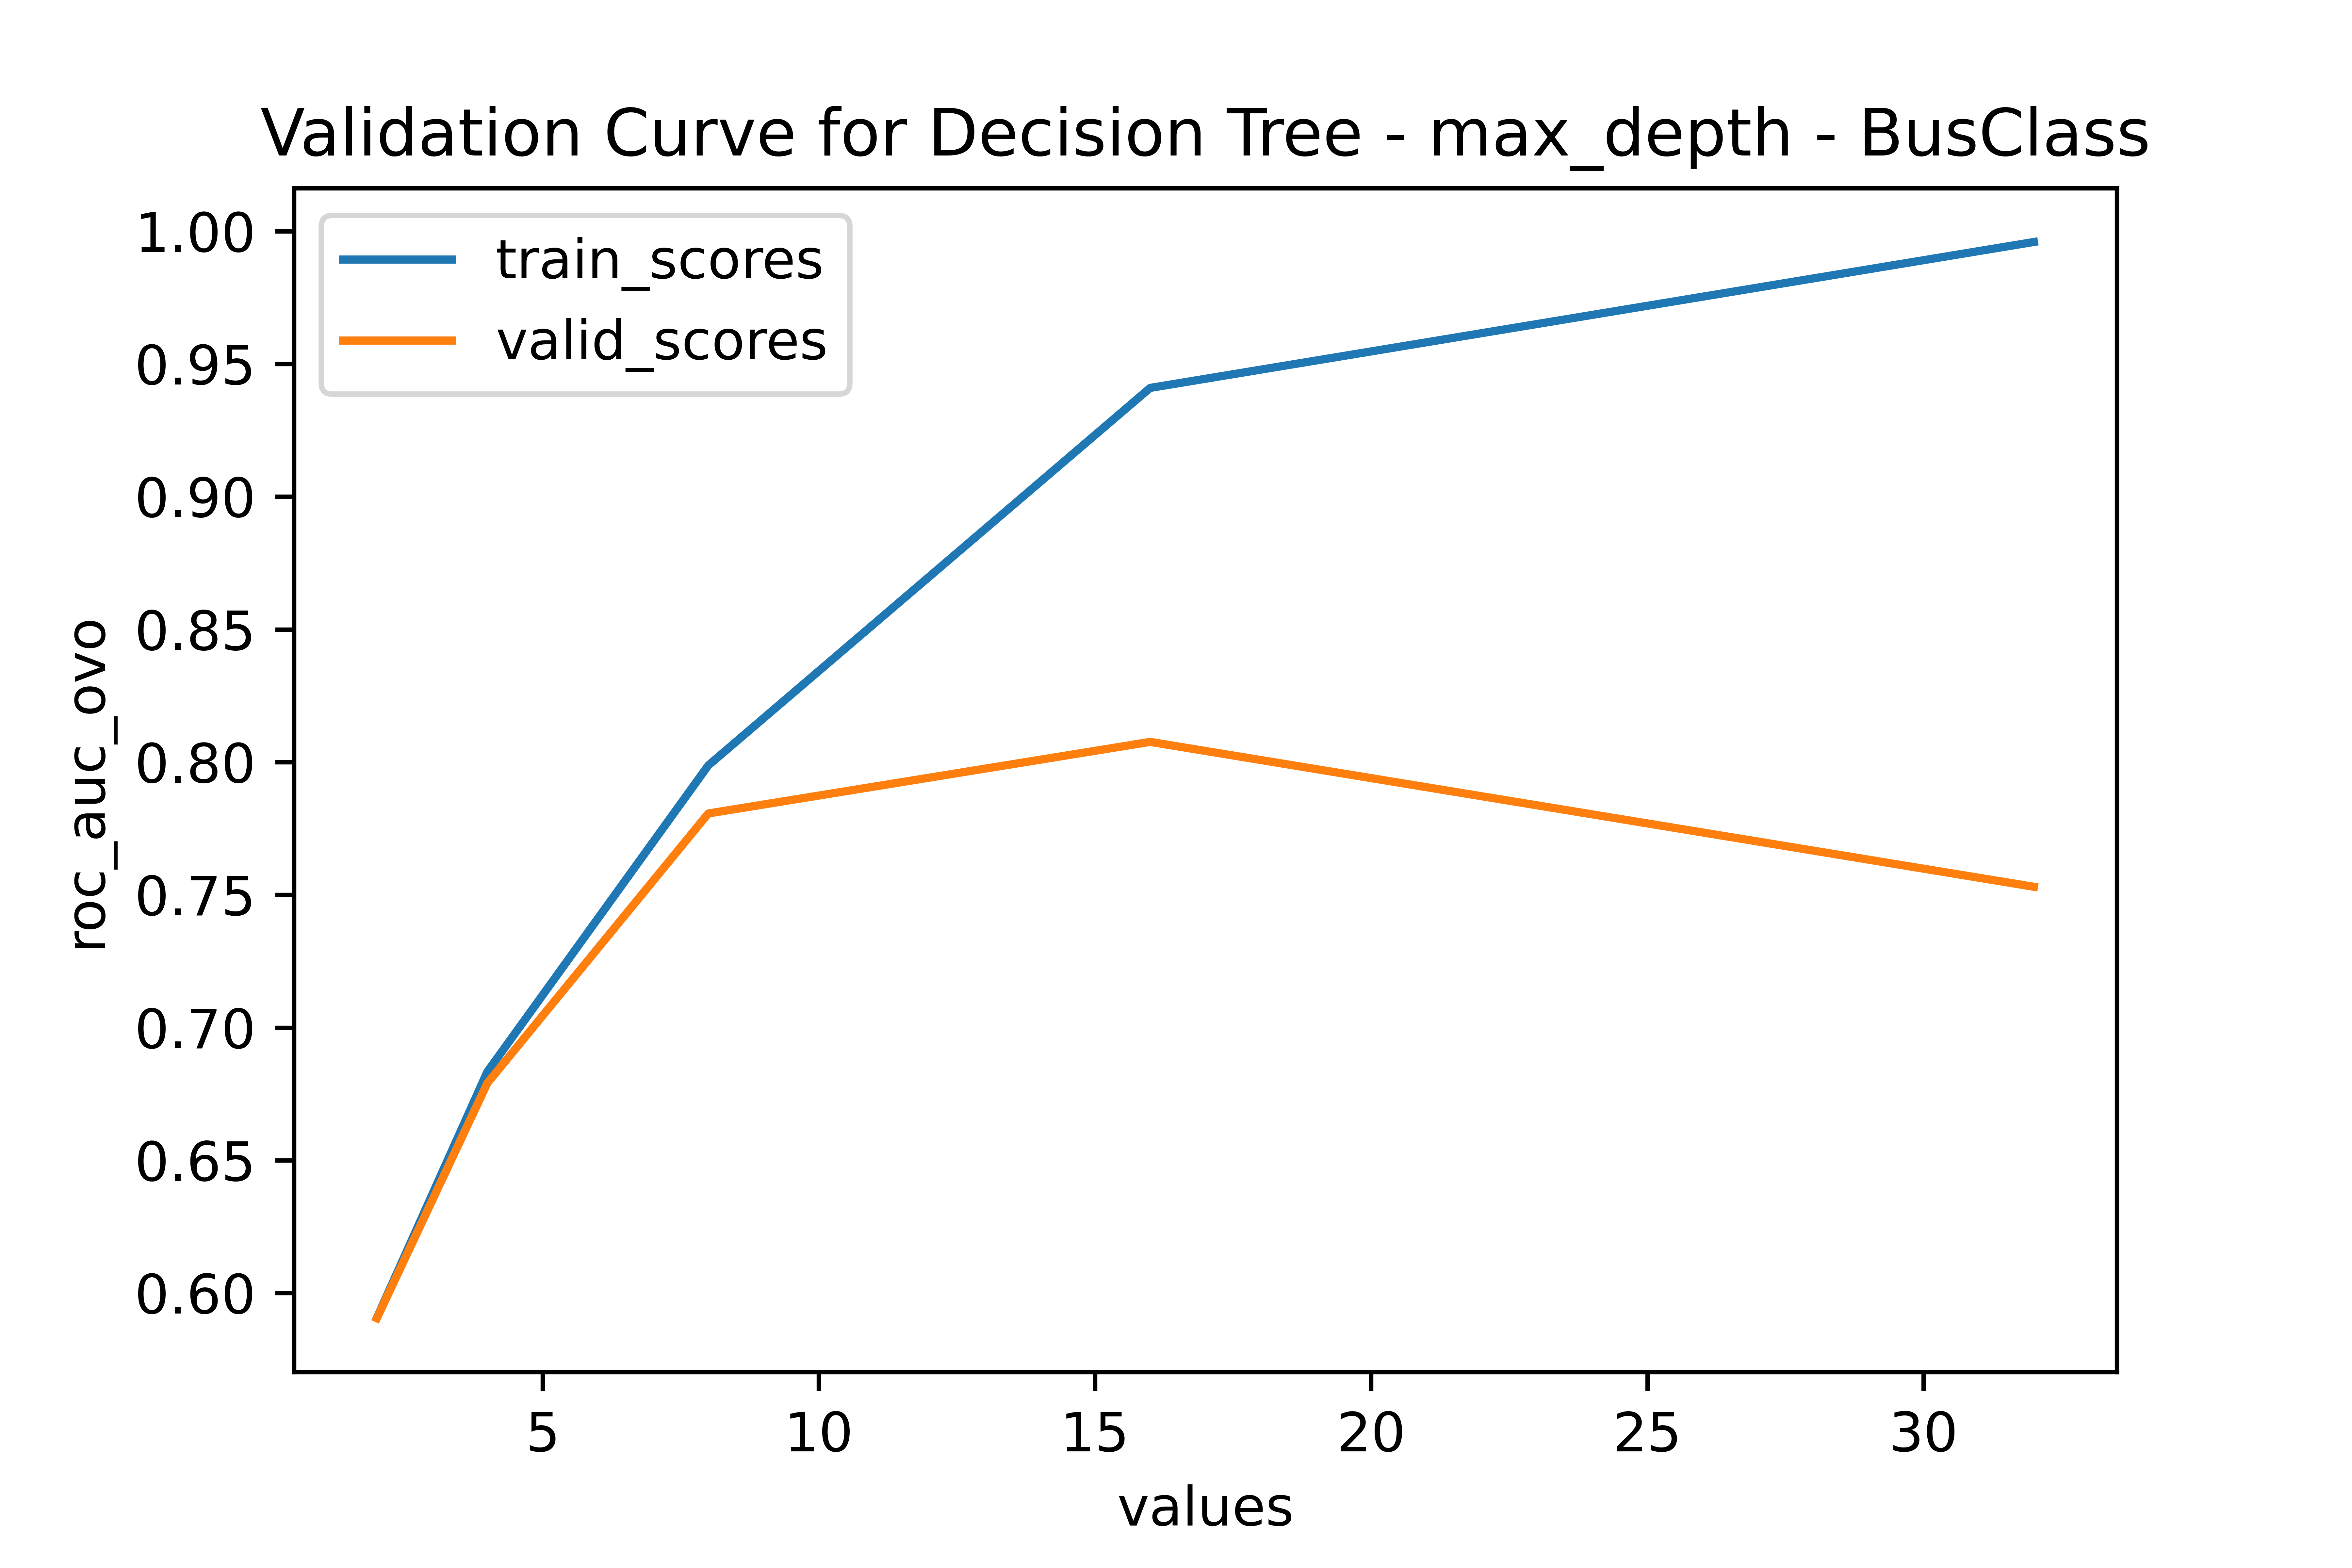
\includegraphics[width=3.4in]{Figures/BusClass-0920/DT/val_curve_0.png}
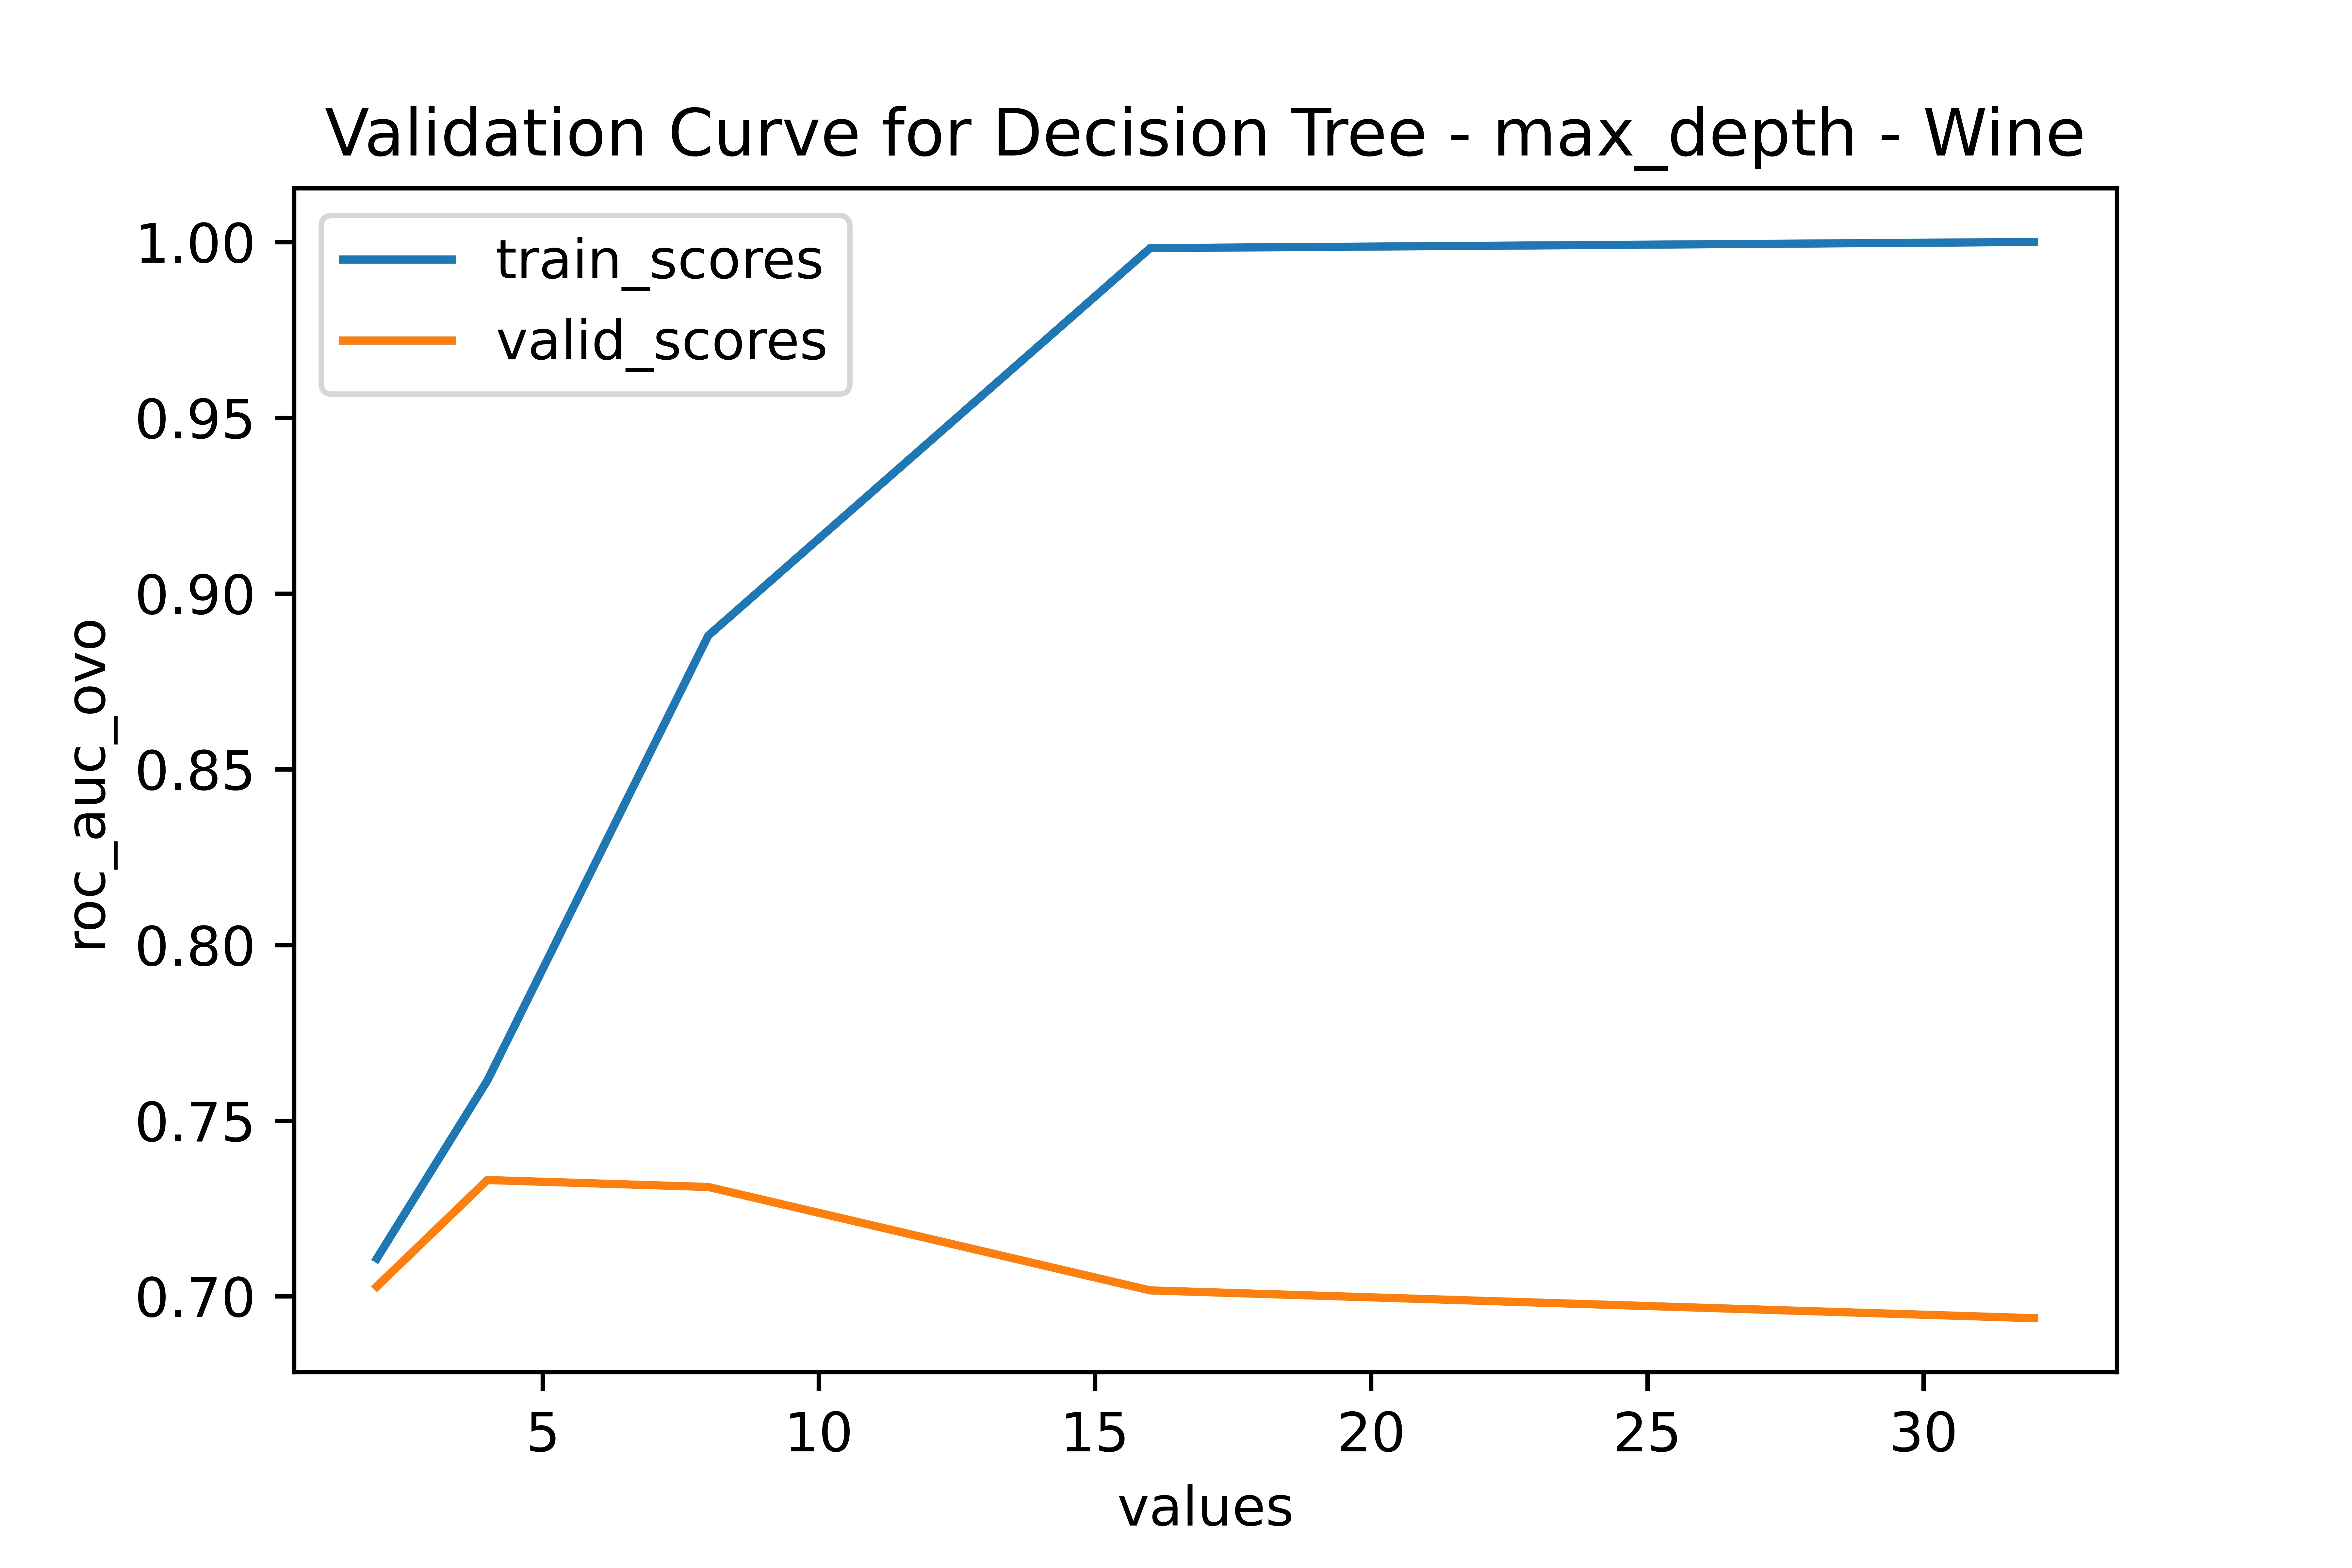
\includegraphics[width=3.4in]{Figures/Wine-0921/DT/val_curve_0.png}

We also wanted to examine the benefit of pruning on our models and find that their optimal values happen to align. This implies that a small amount of pruning is recommended for both the classifiers. The high pruning values (as represented by the CCP Alpha hyperparameter) bring the models to score a roughly 0.5 AUC OvO value, which makes sense: as we remove any expressive power from the model by pruning away all subtrees, we no longer have model that differentiates among its inputs.

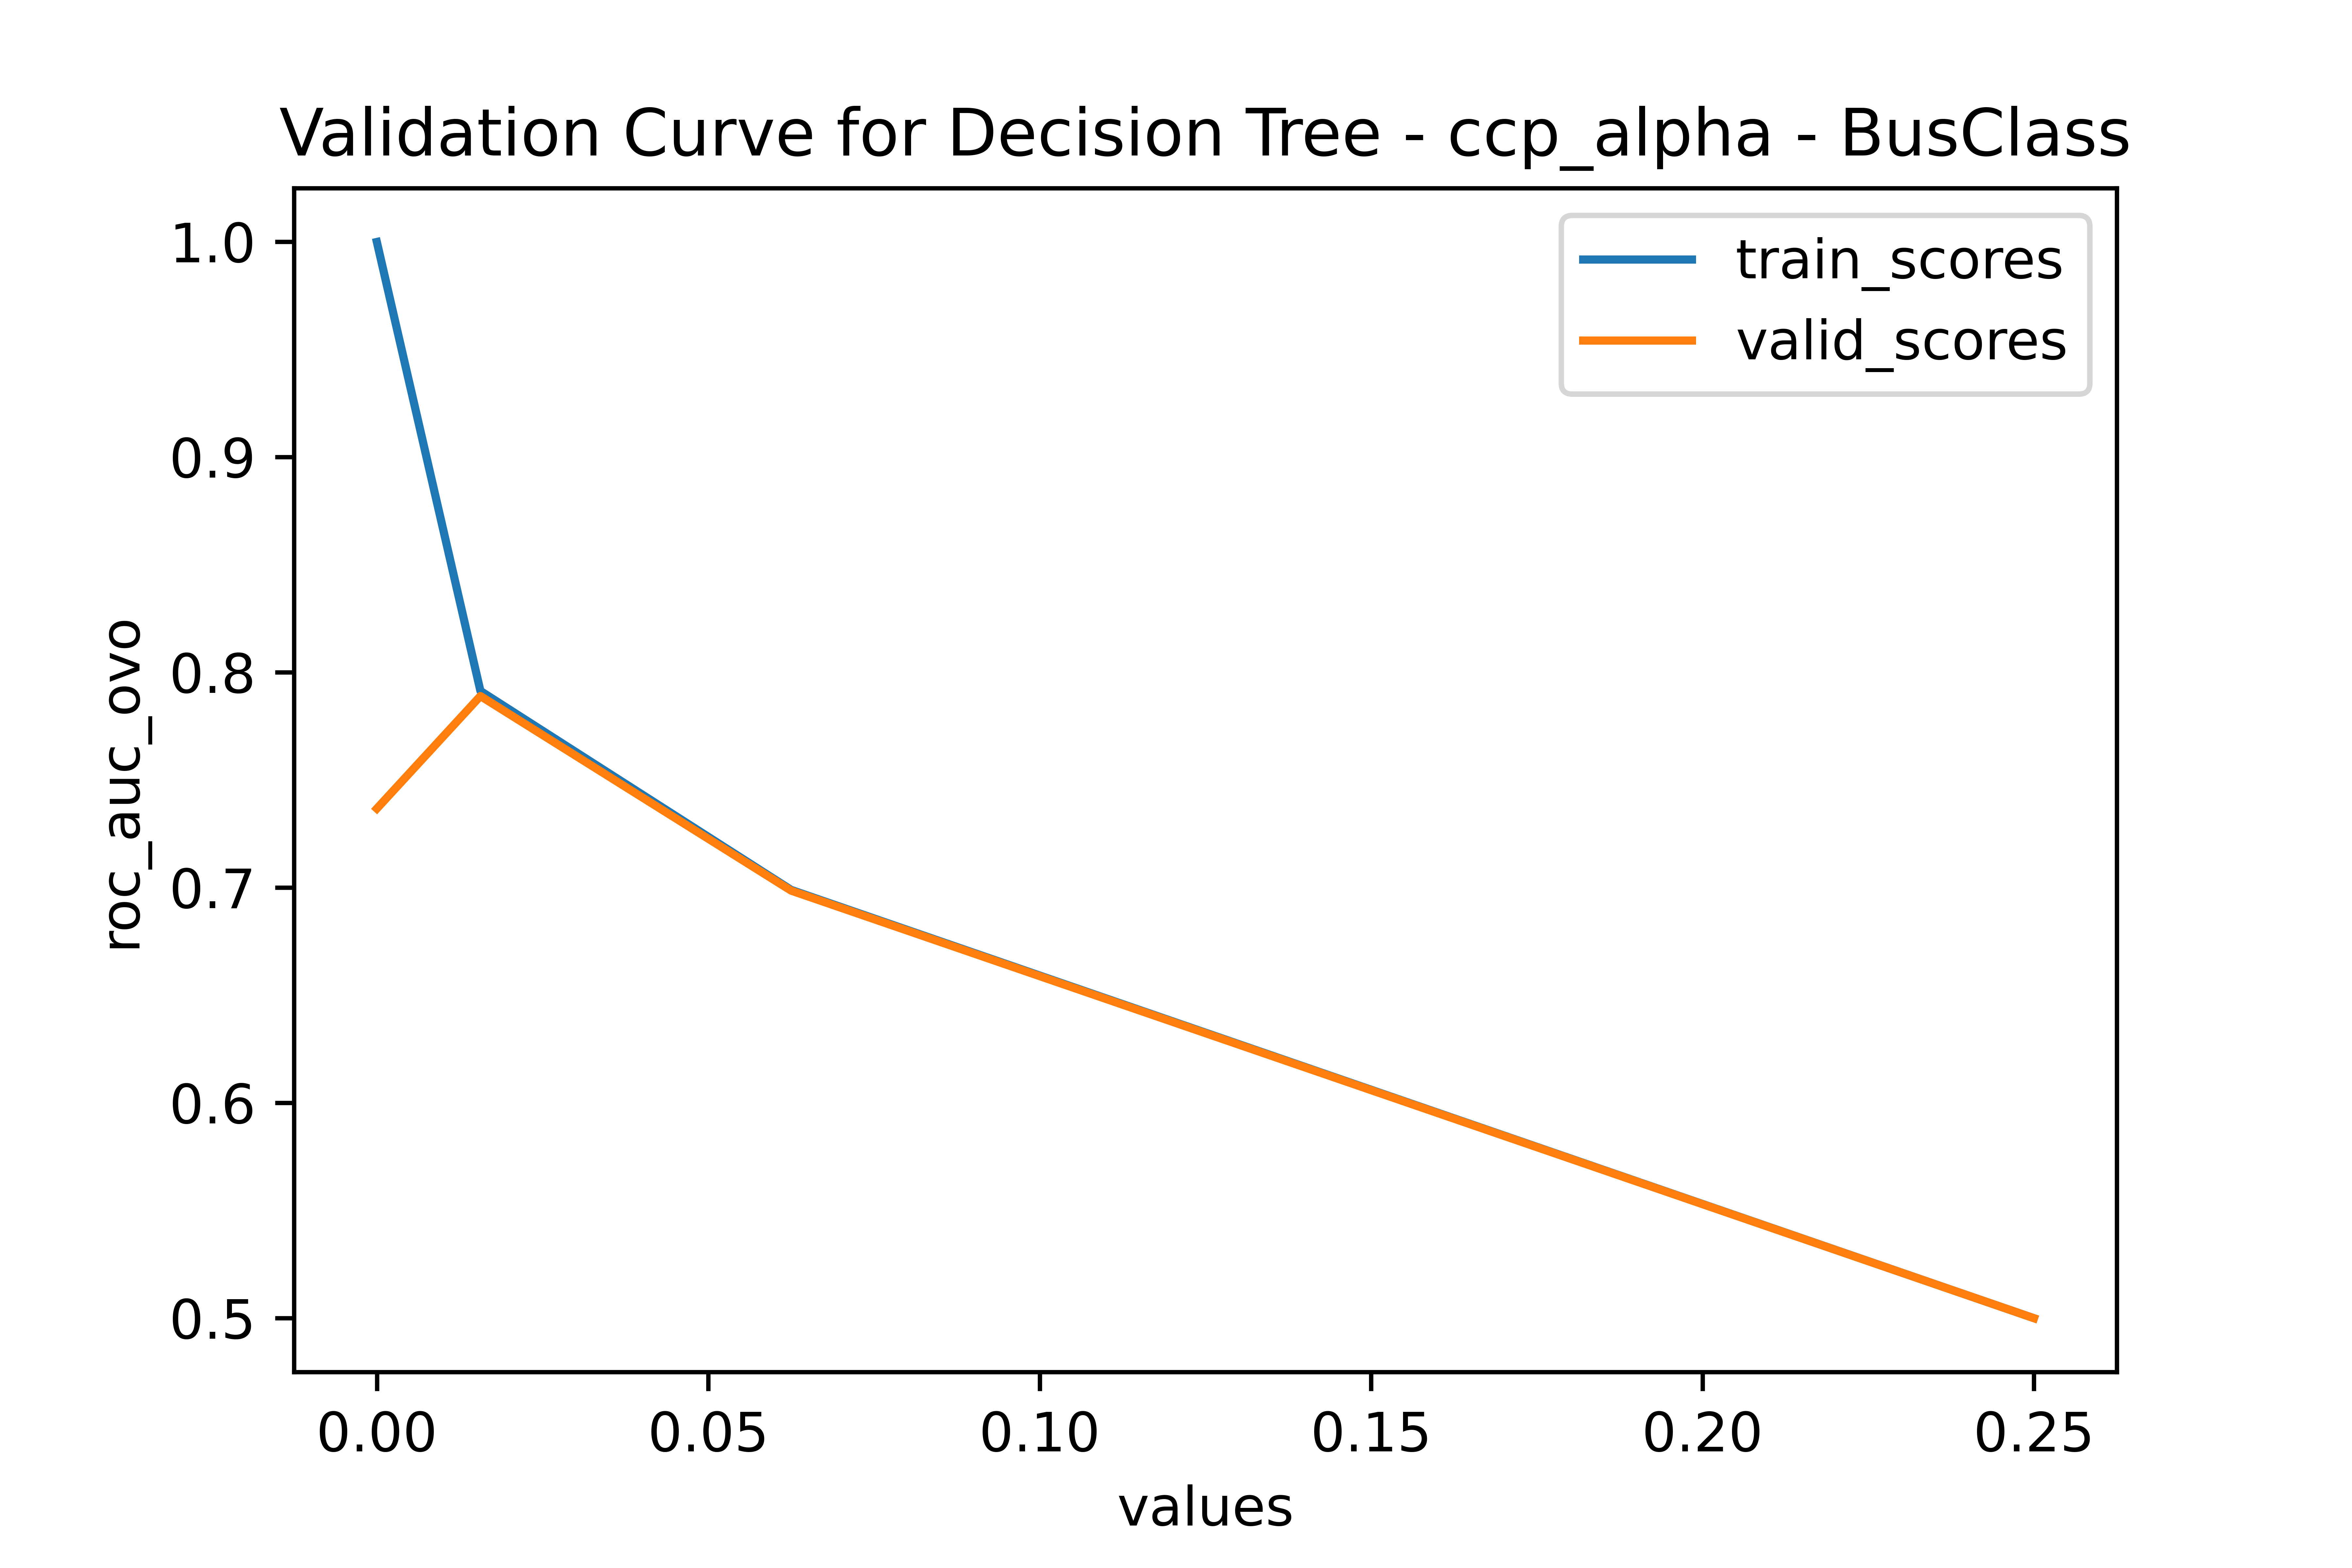
\includegraphics[width=3.4in]{Figures/BusClass-0920/DT/val_curve_1.png}
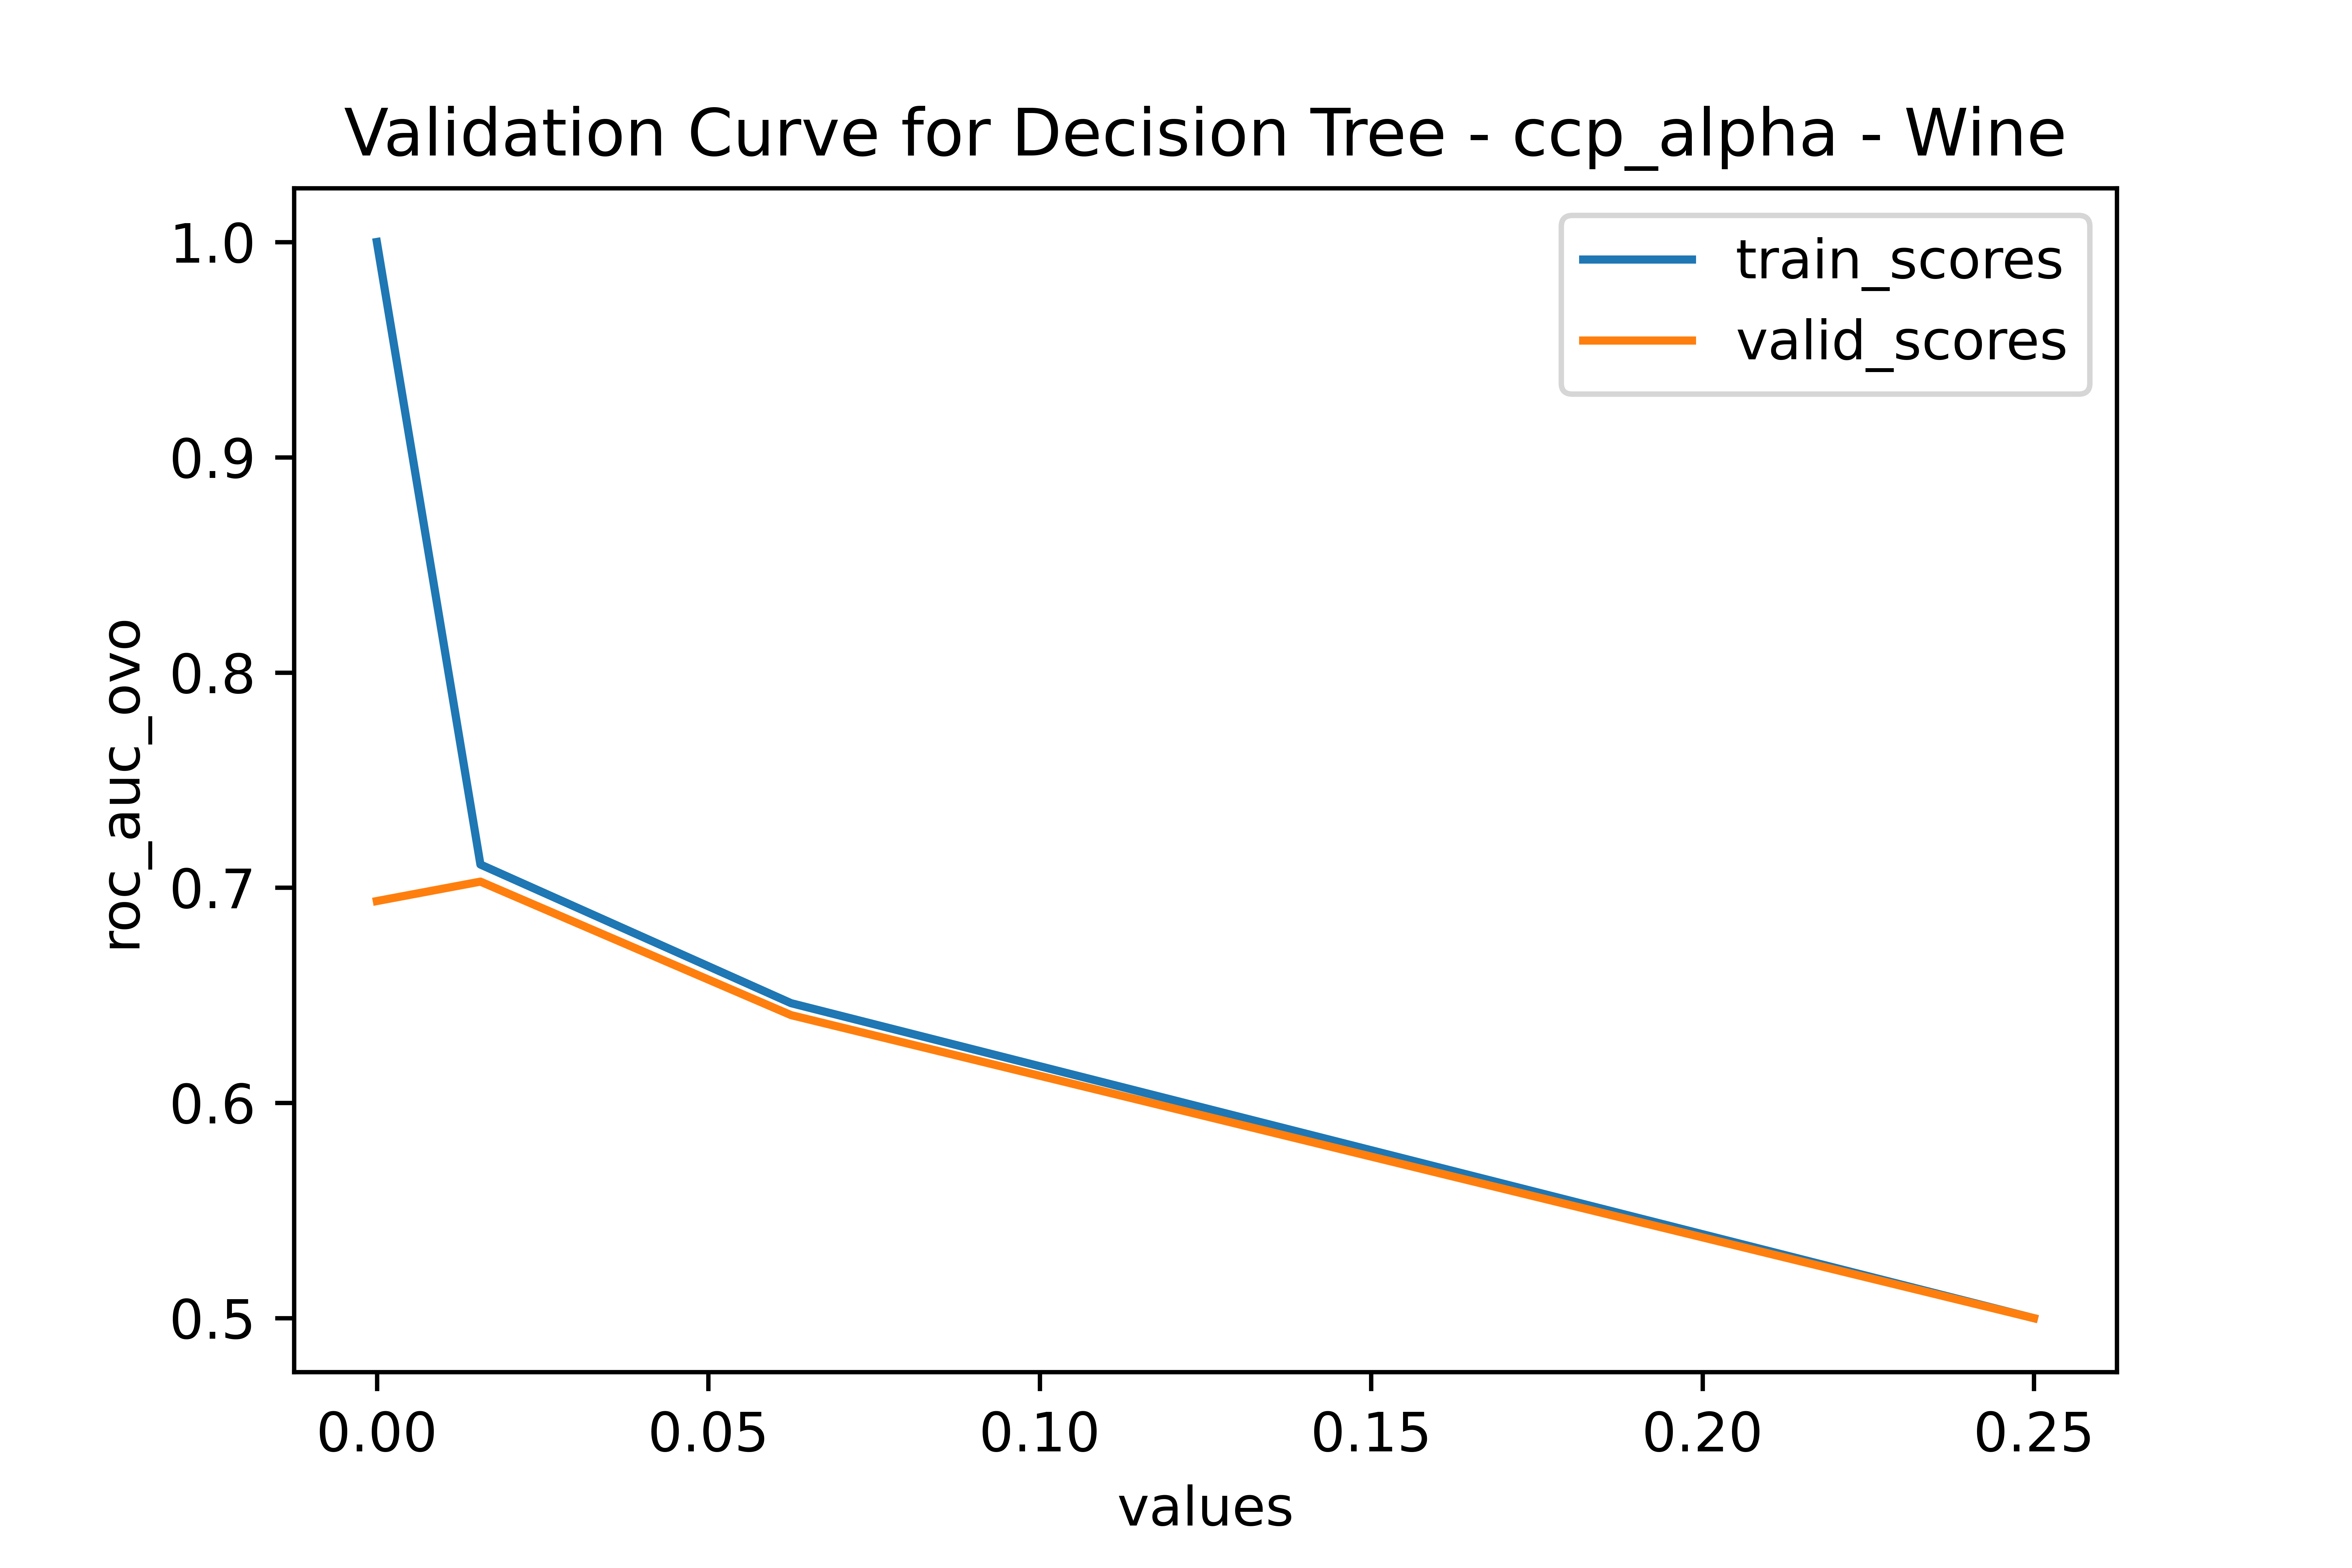
\includegraphics[width=3.4in]{Figures/Wine-0921/DT/val_curve_1.png}

\subsubsection{Learning Curves}
It appears that for the business classification dataset, the model's performance on the validation data does not improve after adding in more training data. Significantly, as we add more training data, we also see lower levels of performance on the training data itself. This could be interpreted by saying that we could overfit the training data even with our not-very-expressive decision tree when there were fewer data points, but cannot with a more general set of data, even data we are training on.

For the wine dataset, though, we see a slightly different pattern. Here performance improves on the validation data after initially adding more training data, but levels off after that relatively early point. This tells me, along with the generally low levels of AUC, that the decision tree has a hard time generalizing given training data and is thus underfit, exhibiting more bias than it ought.

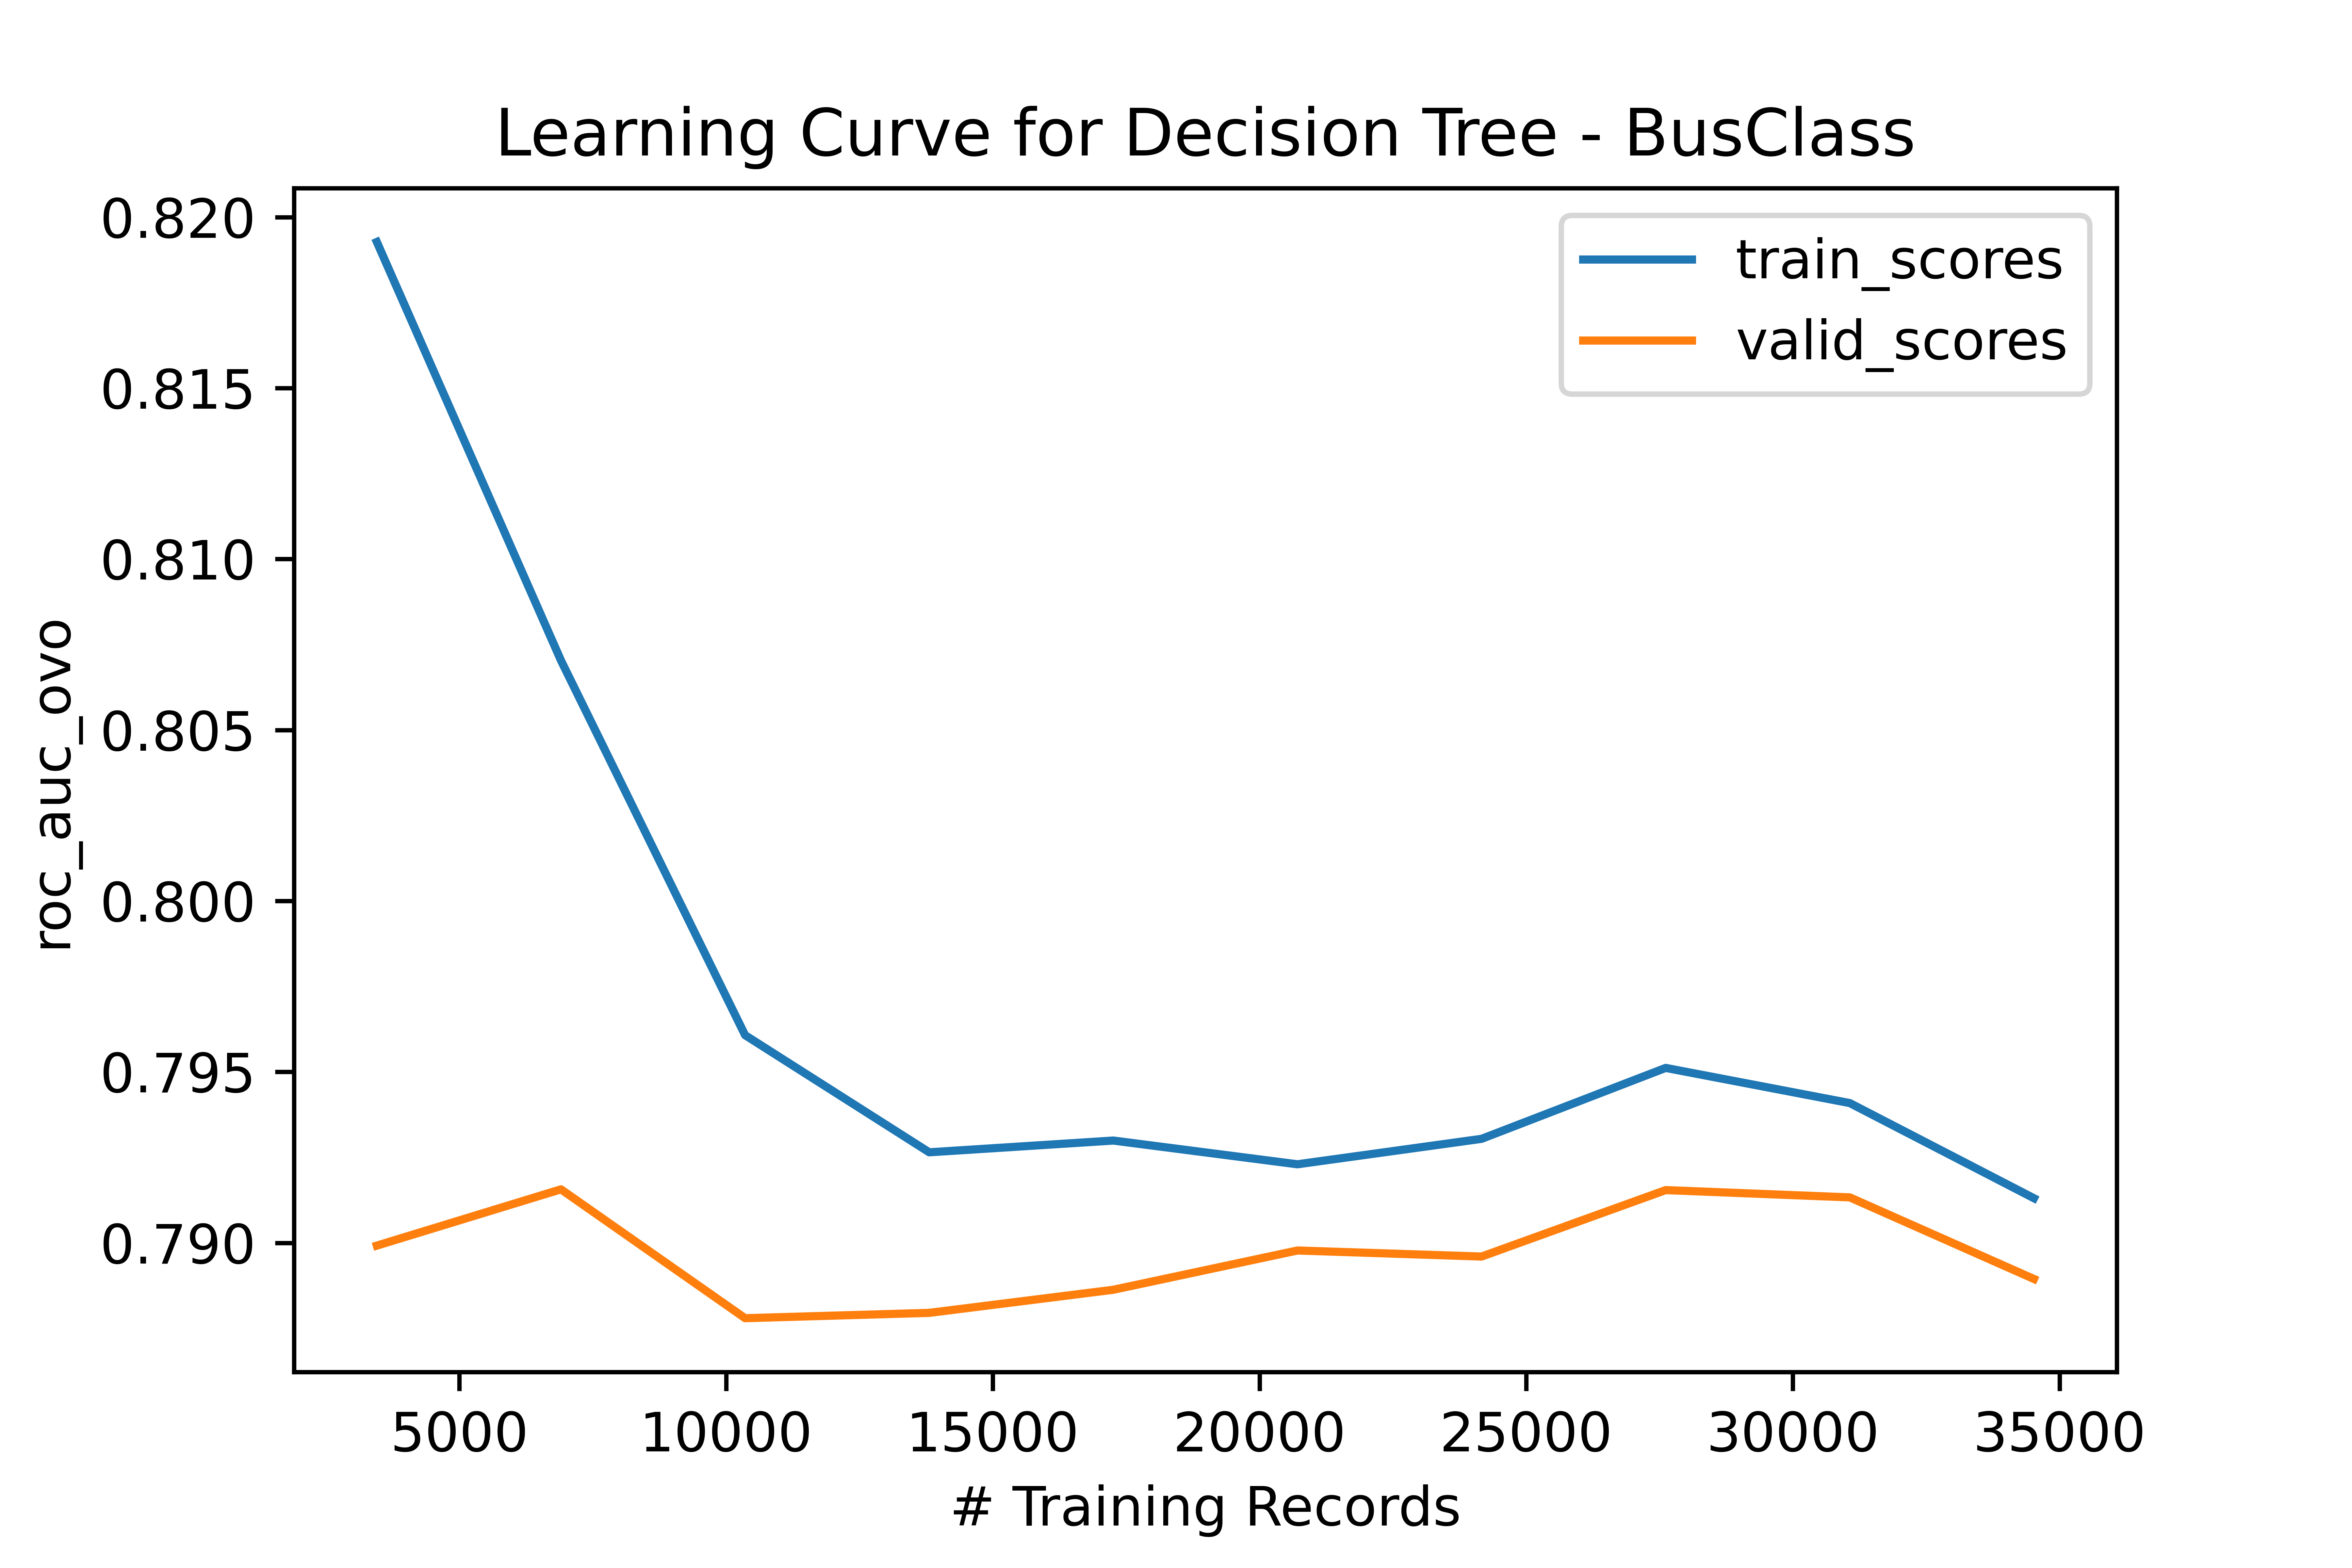
\includegraphics[width=3.4in]{Figures/BusClass-0920/DT/learn_curve.png}
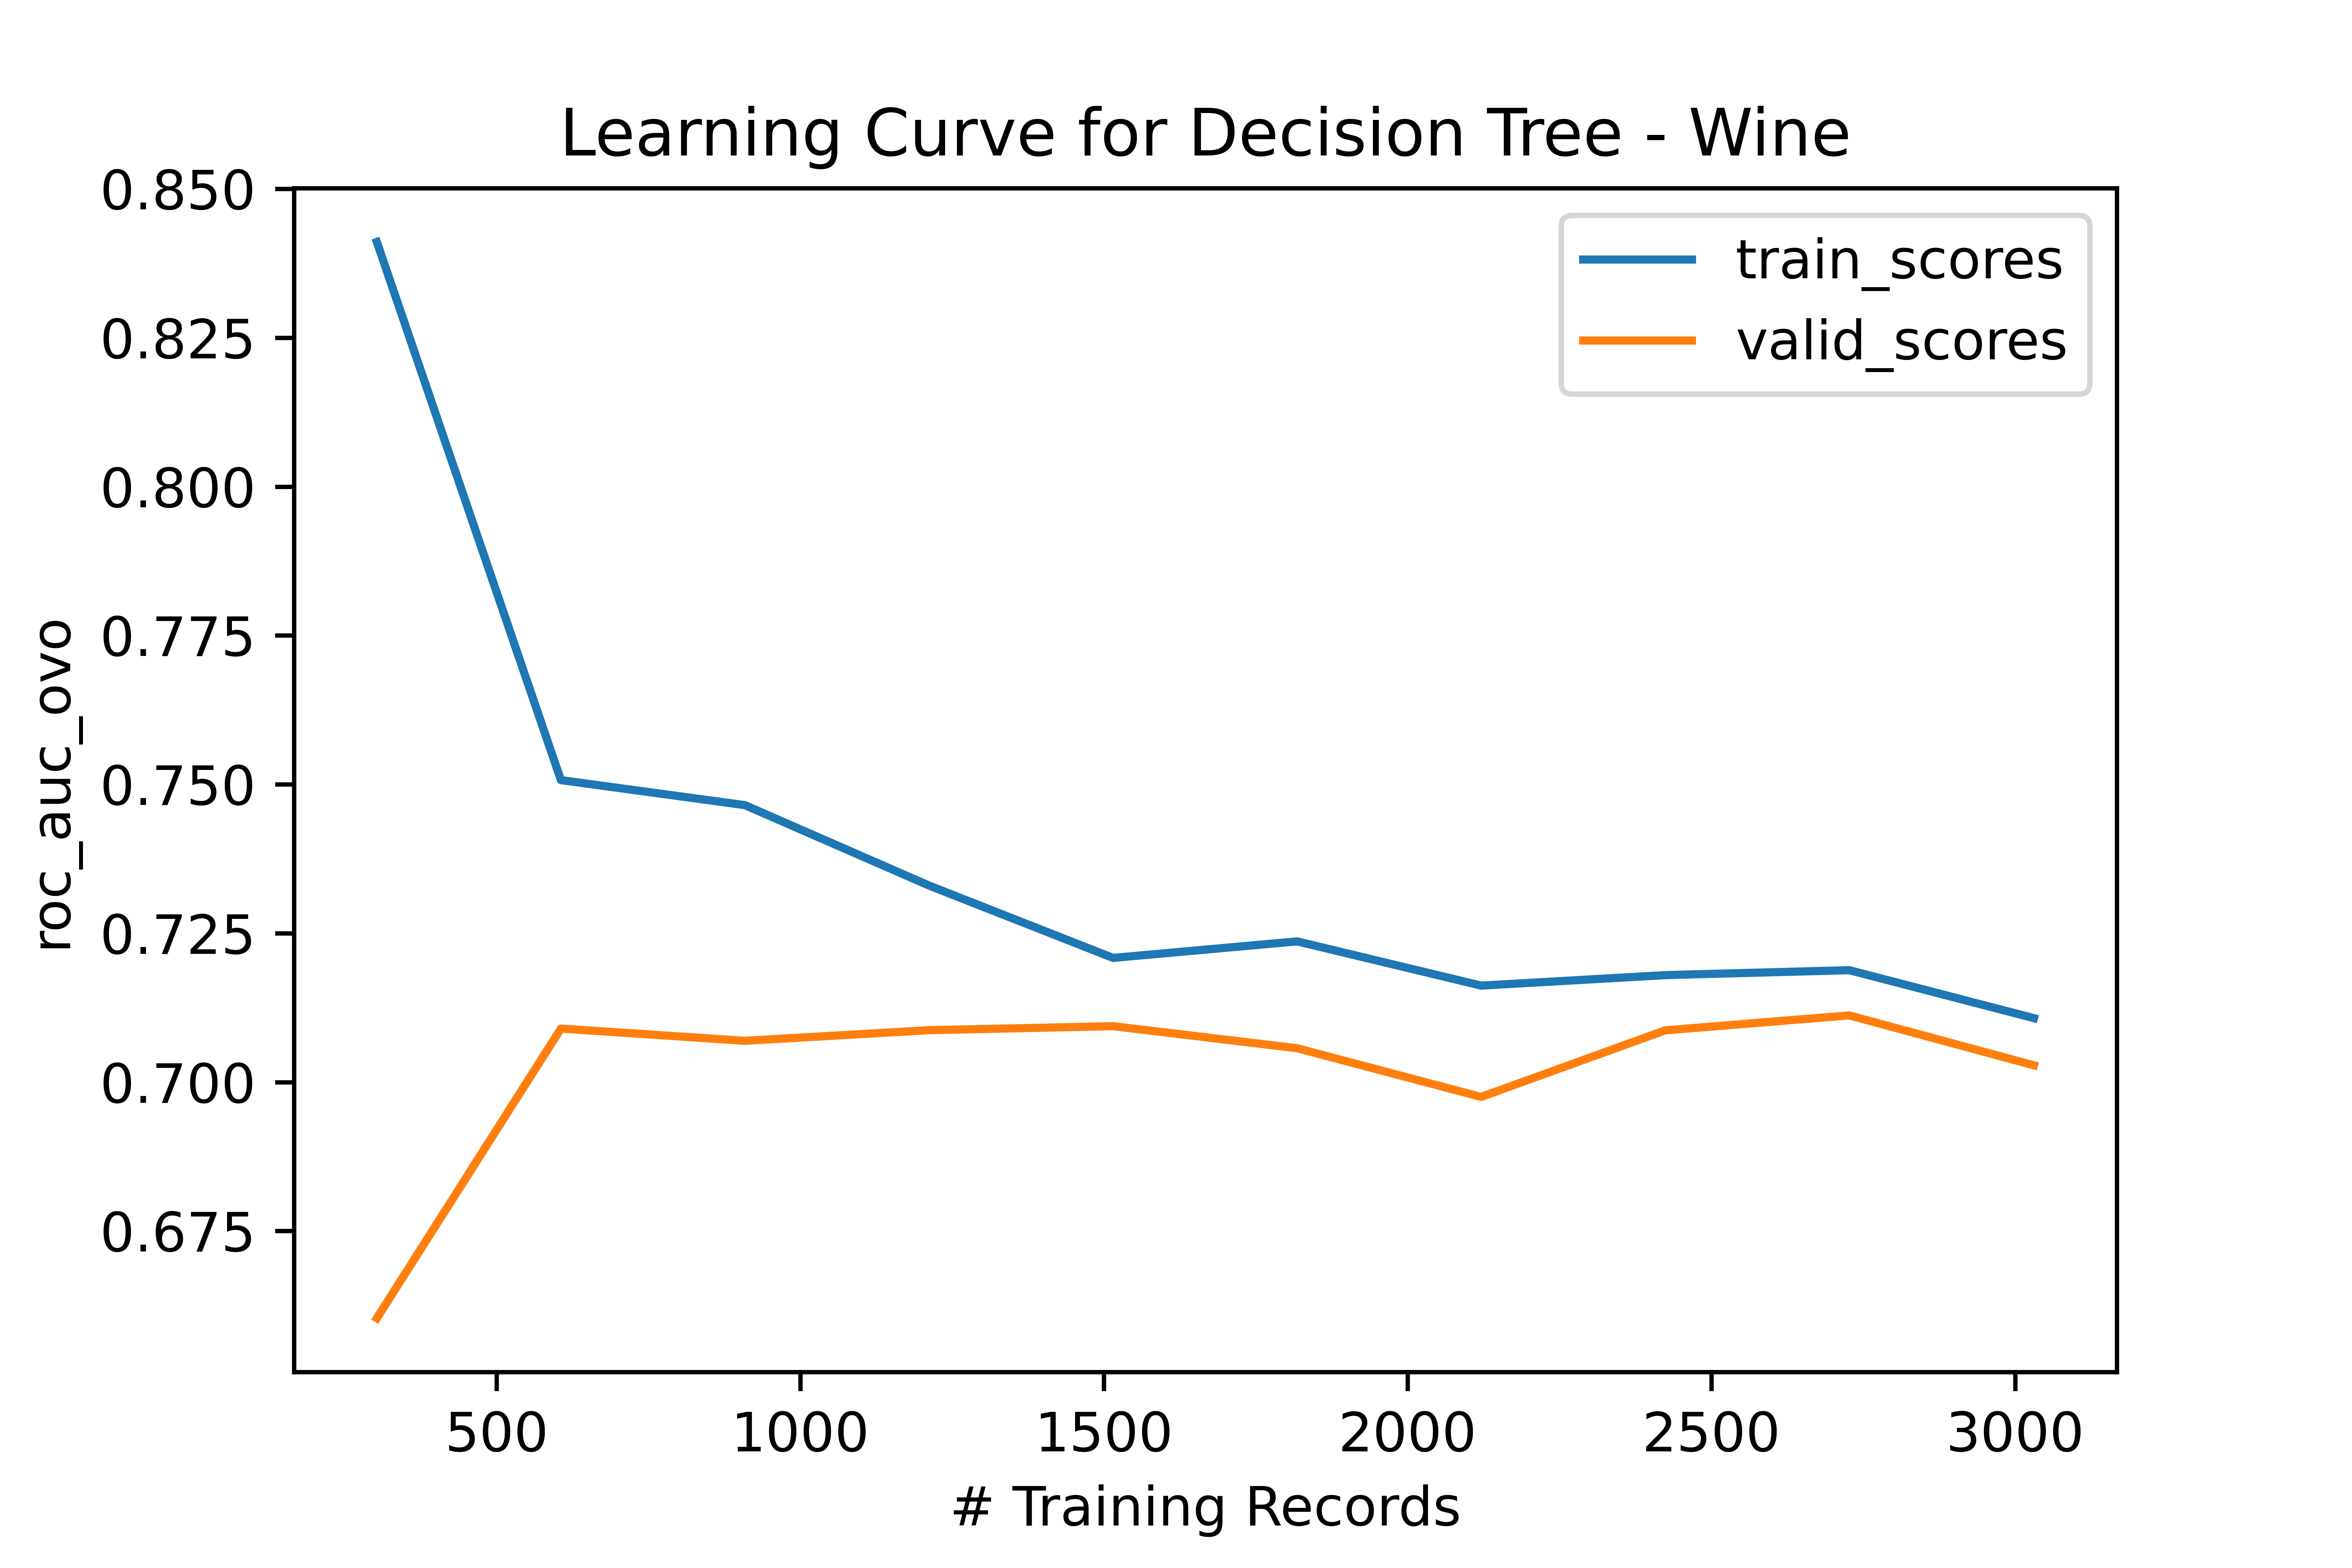
\includegraphics[width=3.4in]{Figures/Wine-0921/DT/learn_curve.png}

\subsubsection{Wall Clock Time}

The algorithm scales roughly linearly in terms of fit time with the amount of training data for the business classification dataset, but this is not the case for the wine dataset. There the algorithm fits very fast for even the whole dataset, probably in part because the tuned model had a relatively small max depth hyperparameter and because the dataset itself was much smaller. Prediction also seems to take constant time.

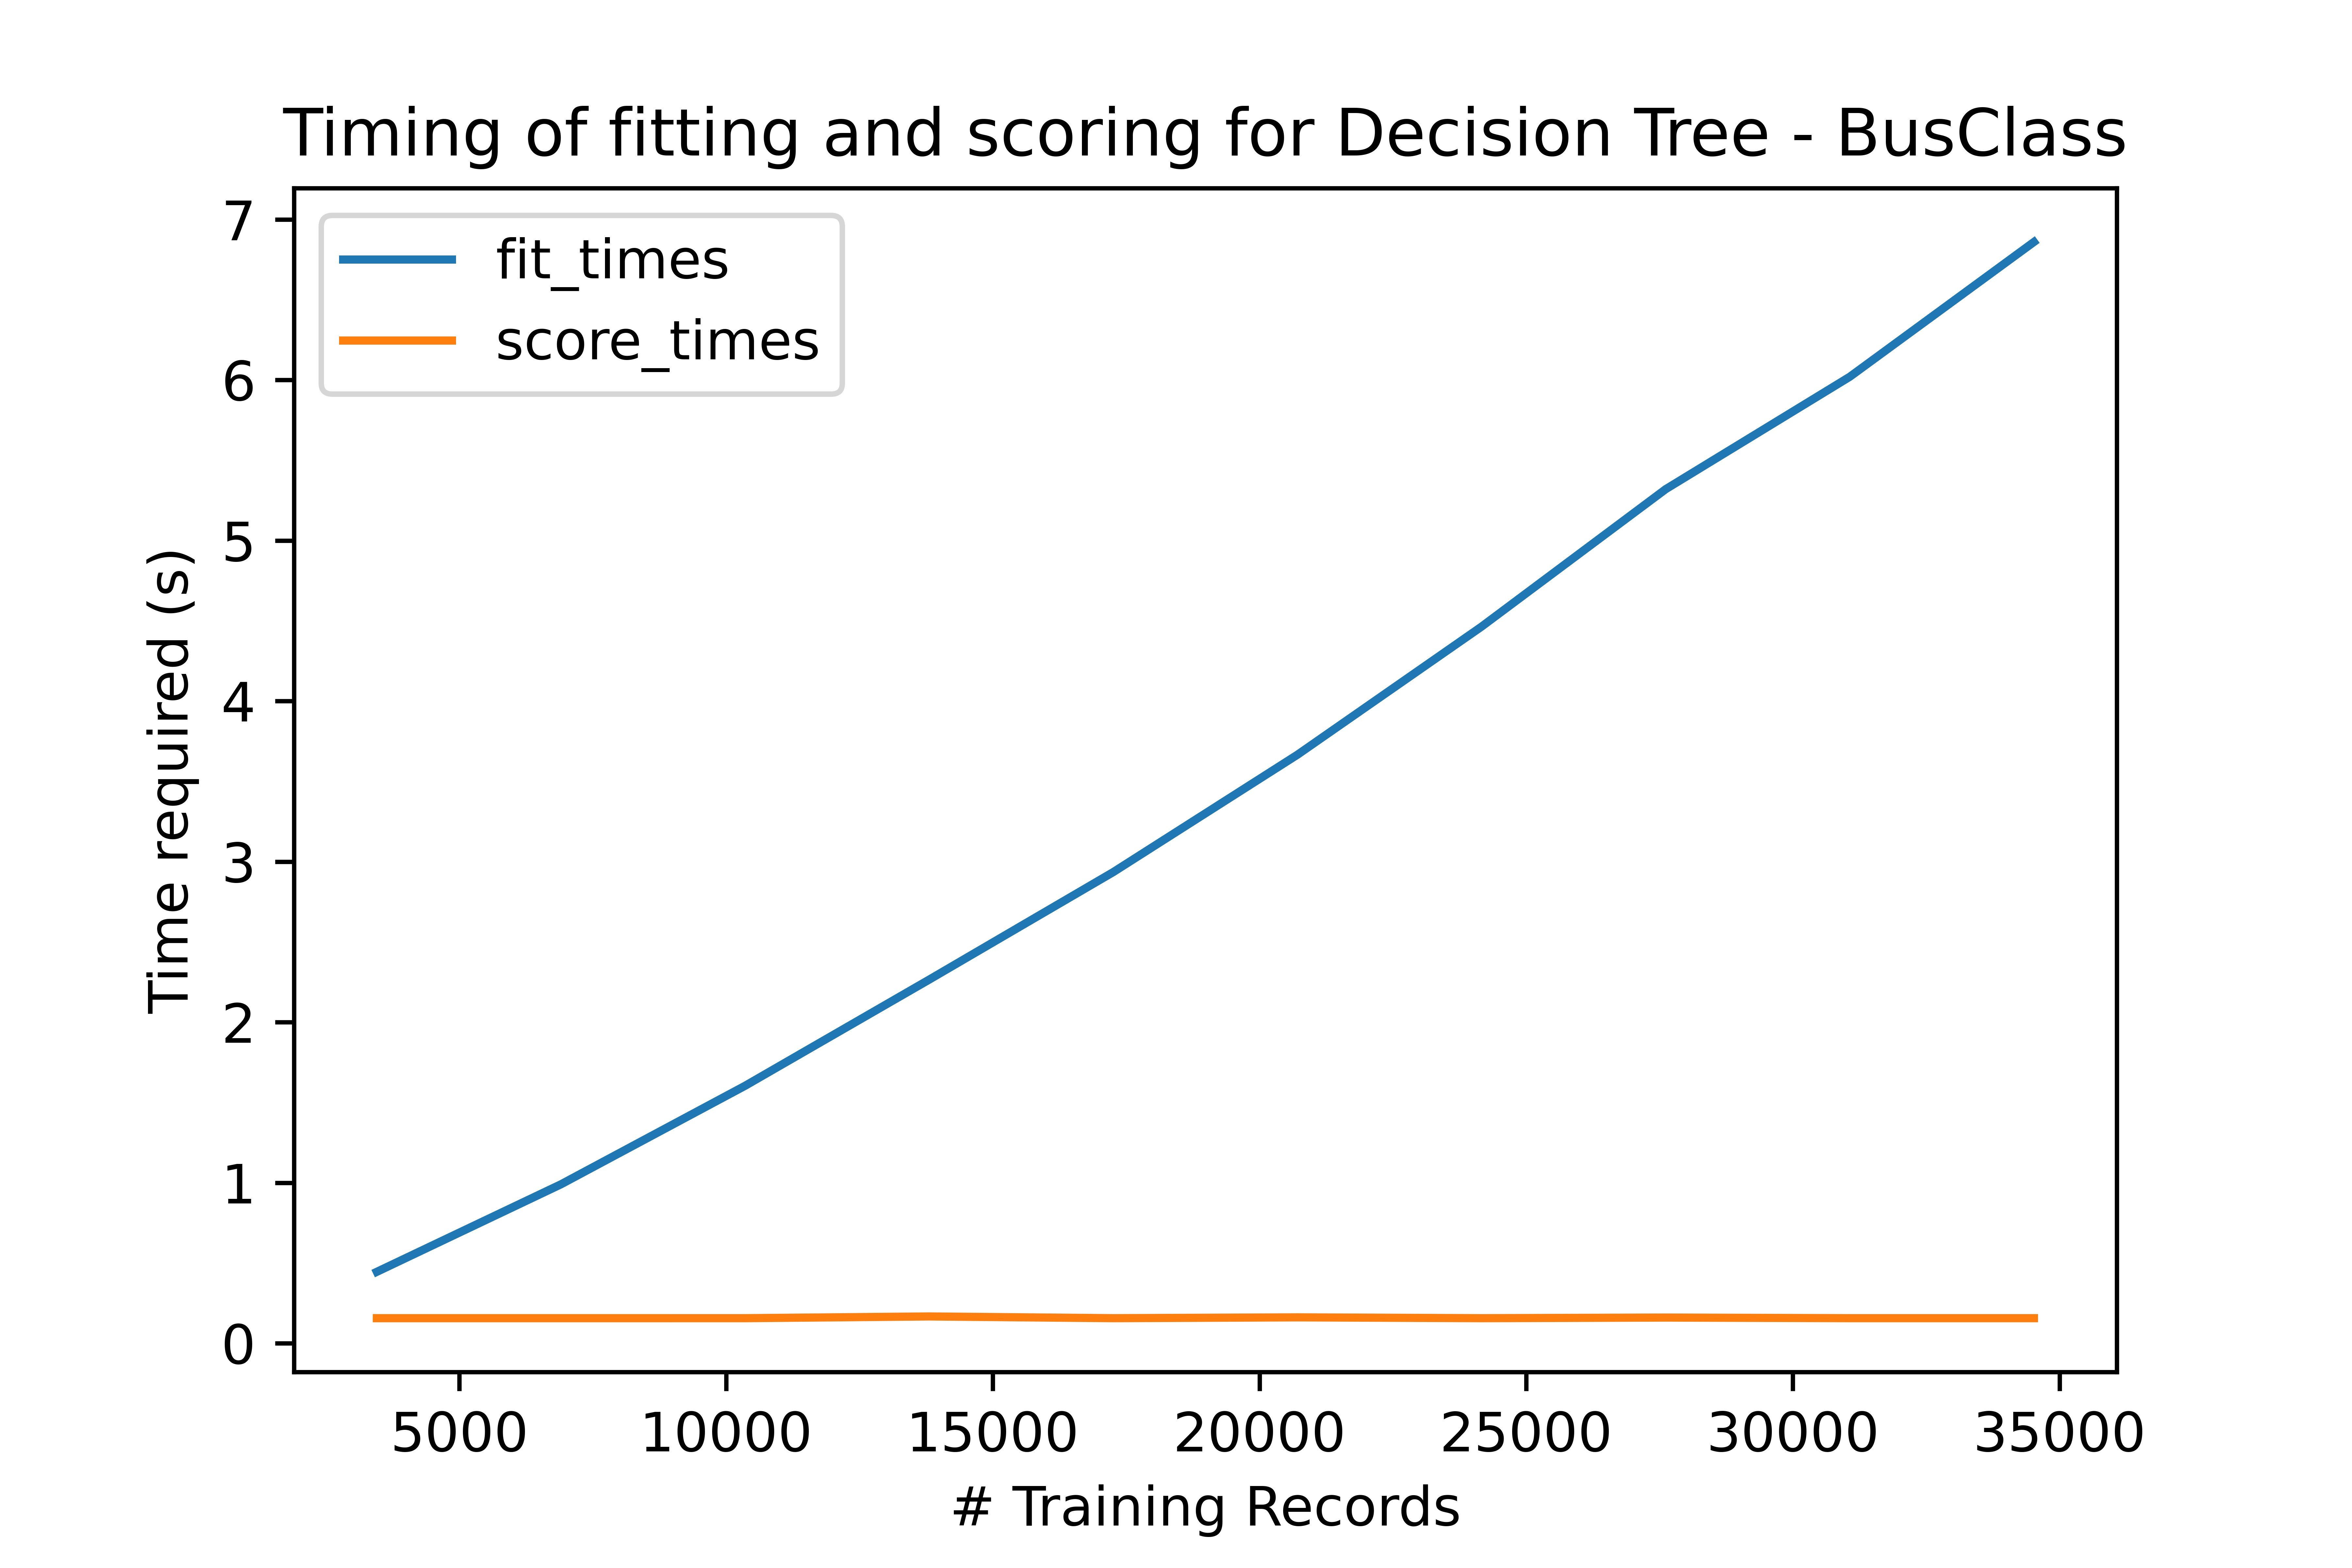
\includegraphics[width=3.4in]{Figures/BusClass-0920/DT/time_curve.png}
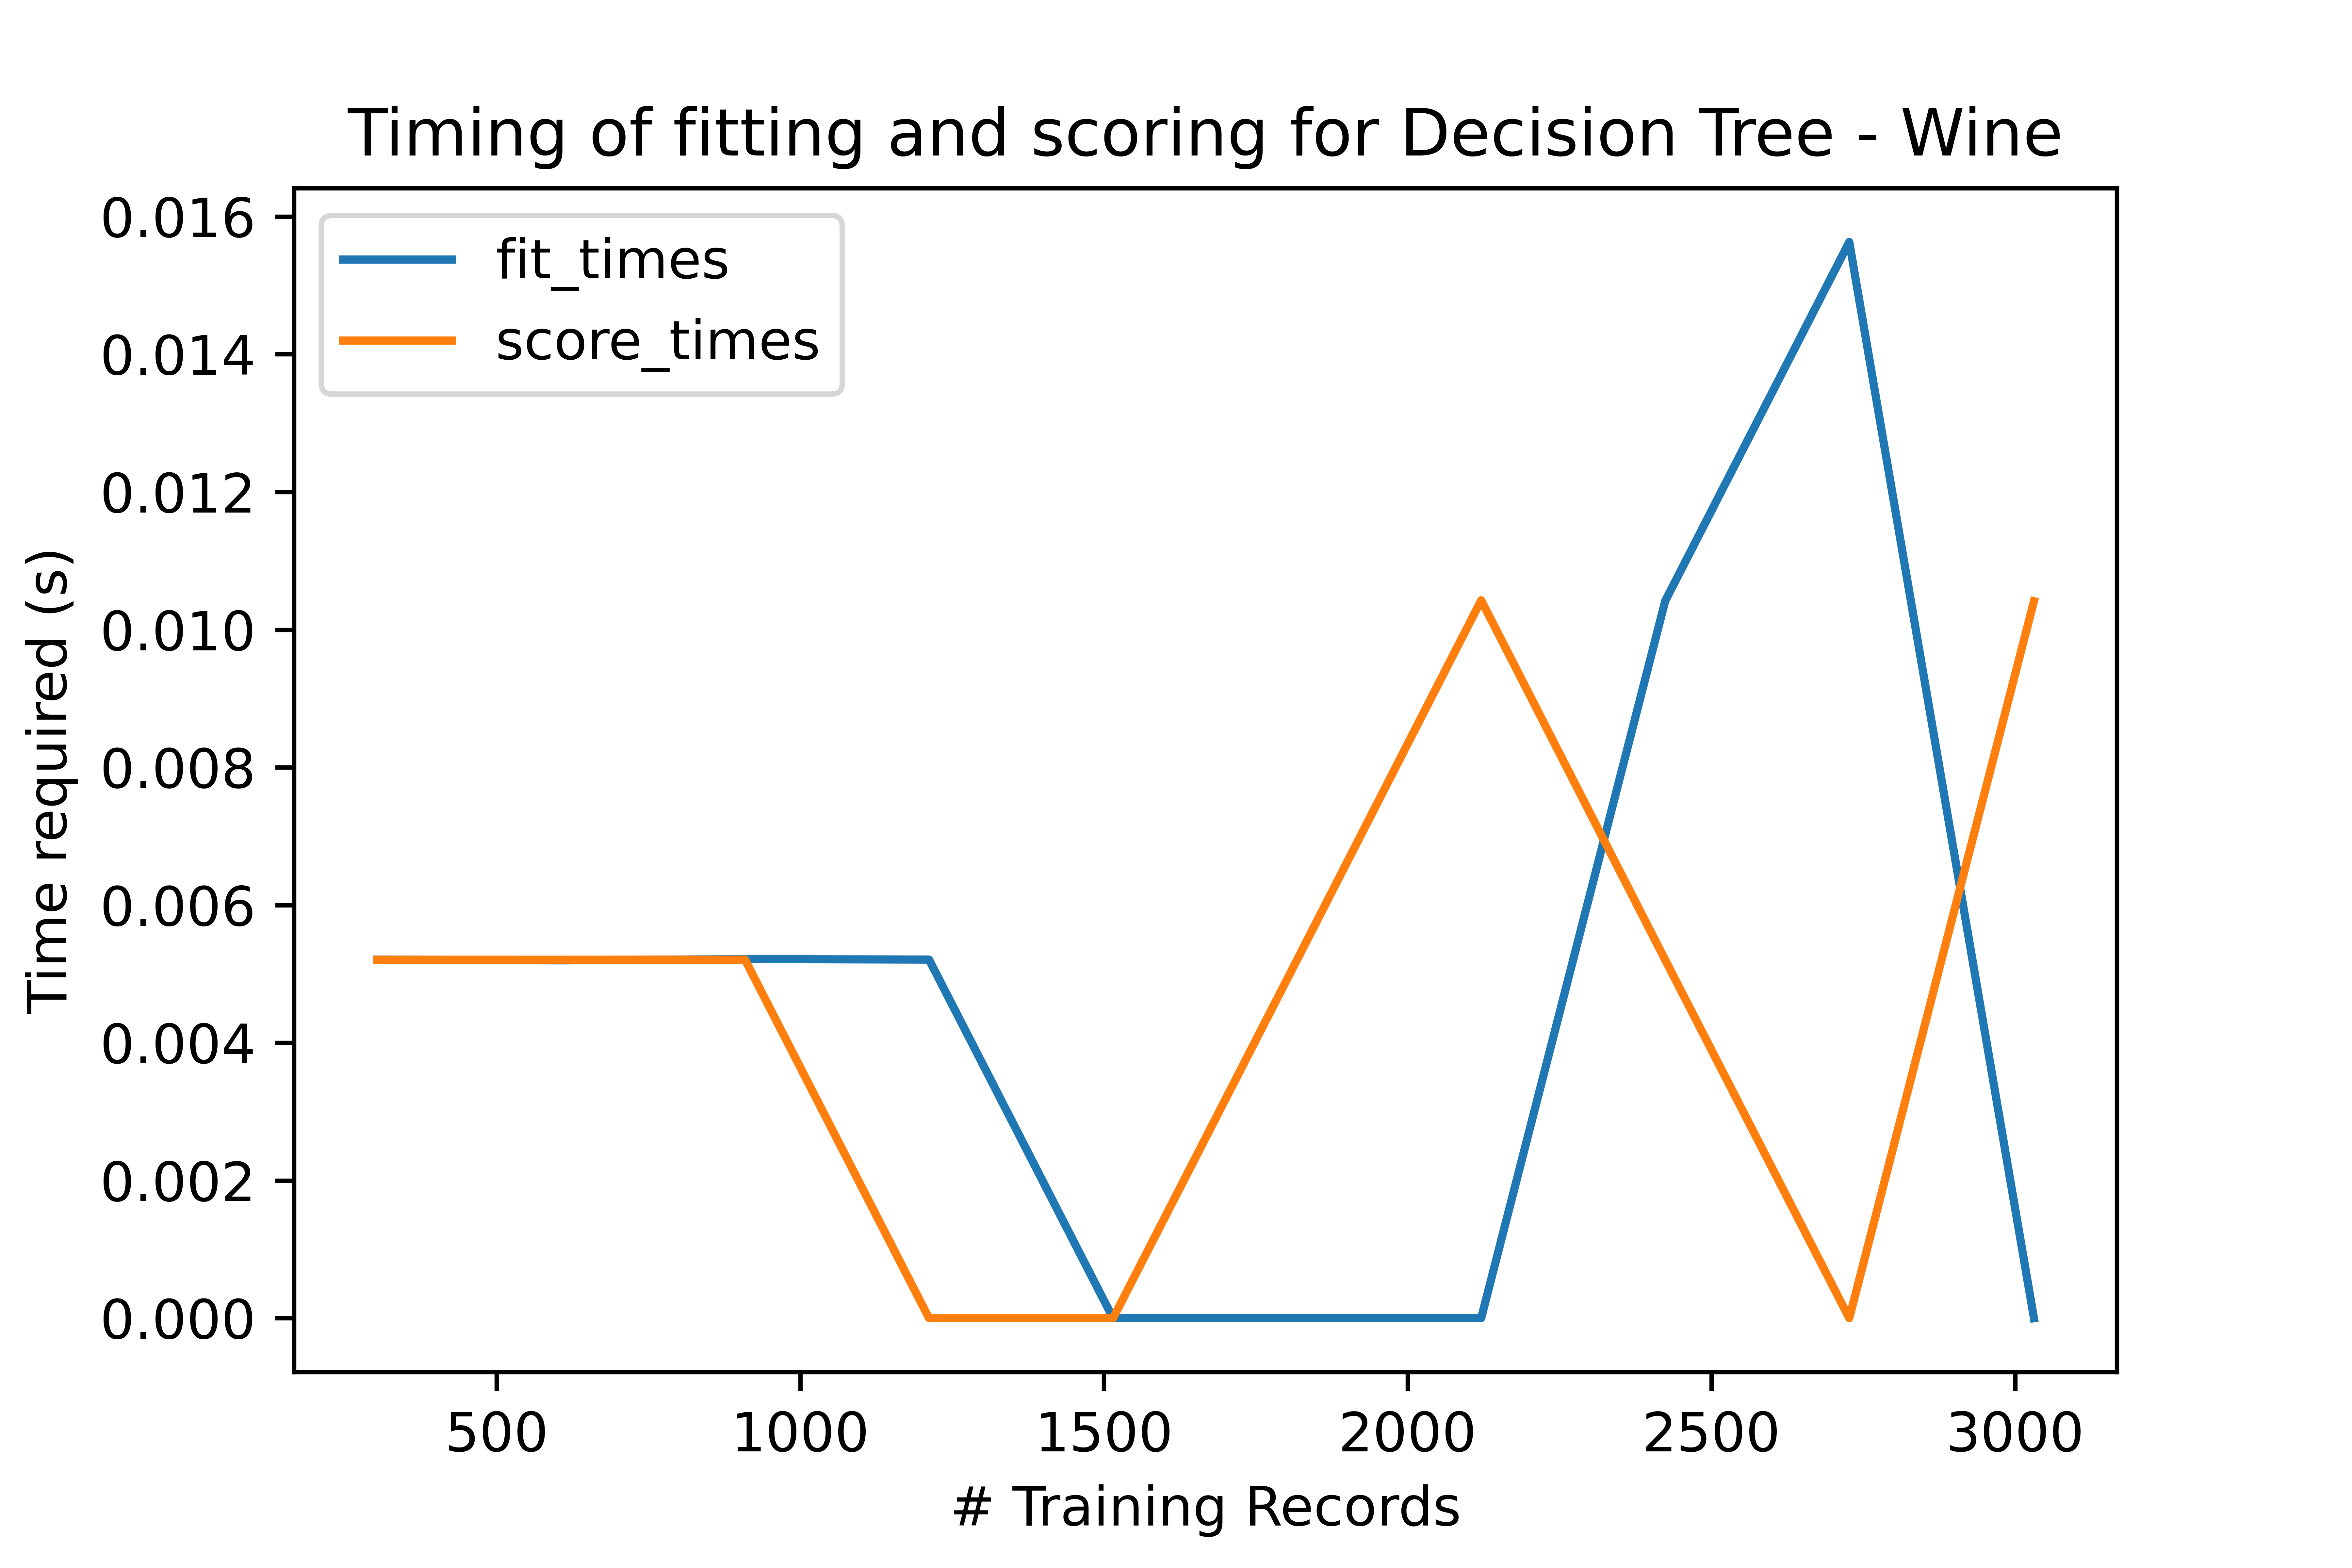
\includegraphics[width=3.4in]{Figures/Wine-0921/DT/time_curve.png}

\subsection{Neural Network}

\subsubsection{Hyperparameter Tuning}

The neural network performed well on the business classification task. Its scoring was less dependent on the hidden layers and node count than expected, but was highly dependent on alpha, the L2 regularization amount. The optimal value, not unlike the CCP Alpha value tuned for the decision tree, was slightly above 0 for the business classification dataset. However, the optimal value for the wine data was precisely zero.

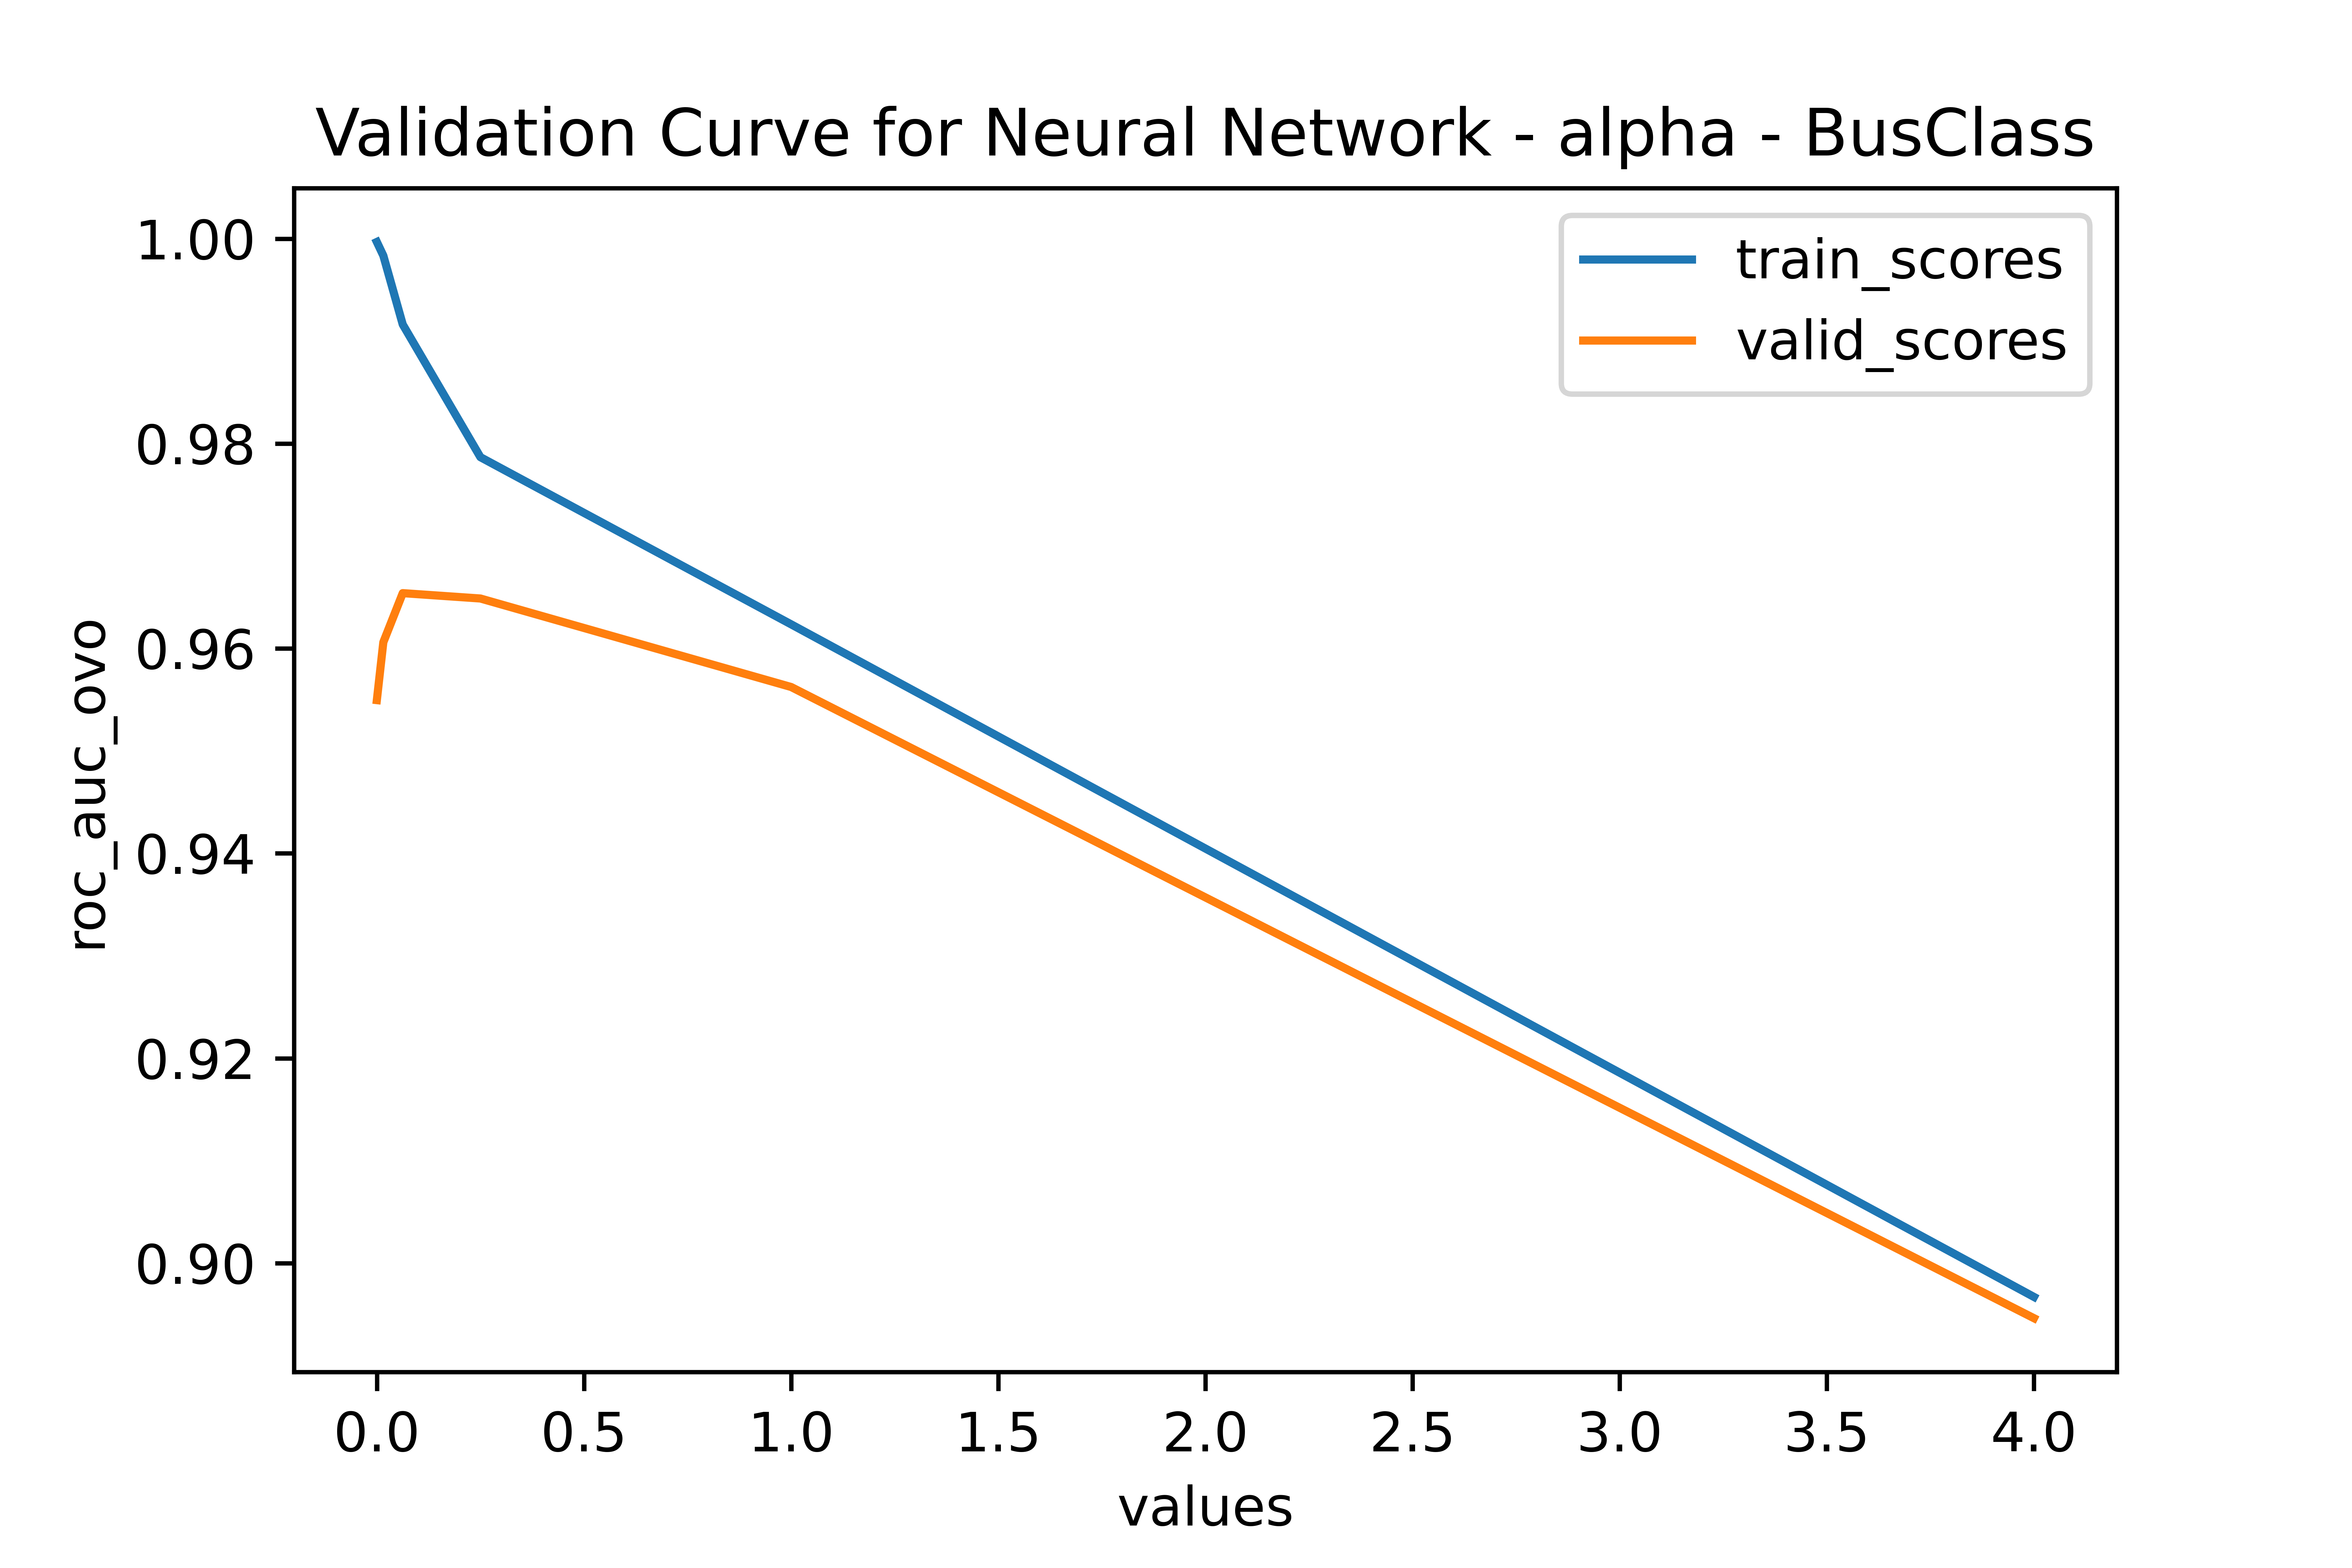
\includegraphics[width=3.4in]{Figures/BusClass-0920/NN/val_curve_0.png}
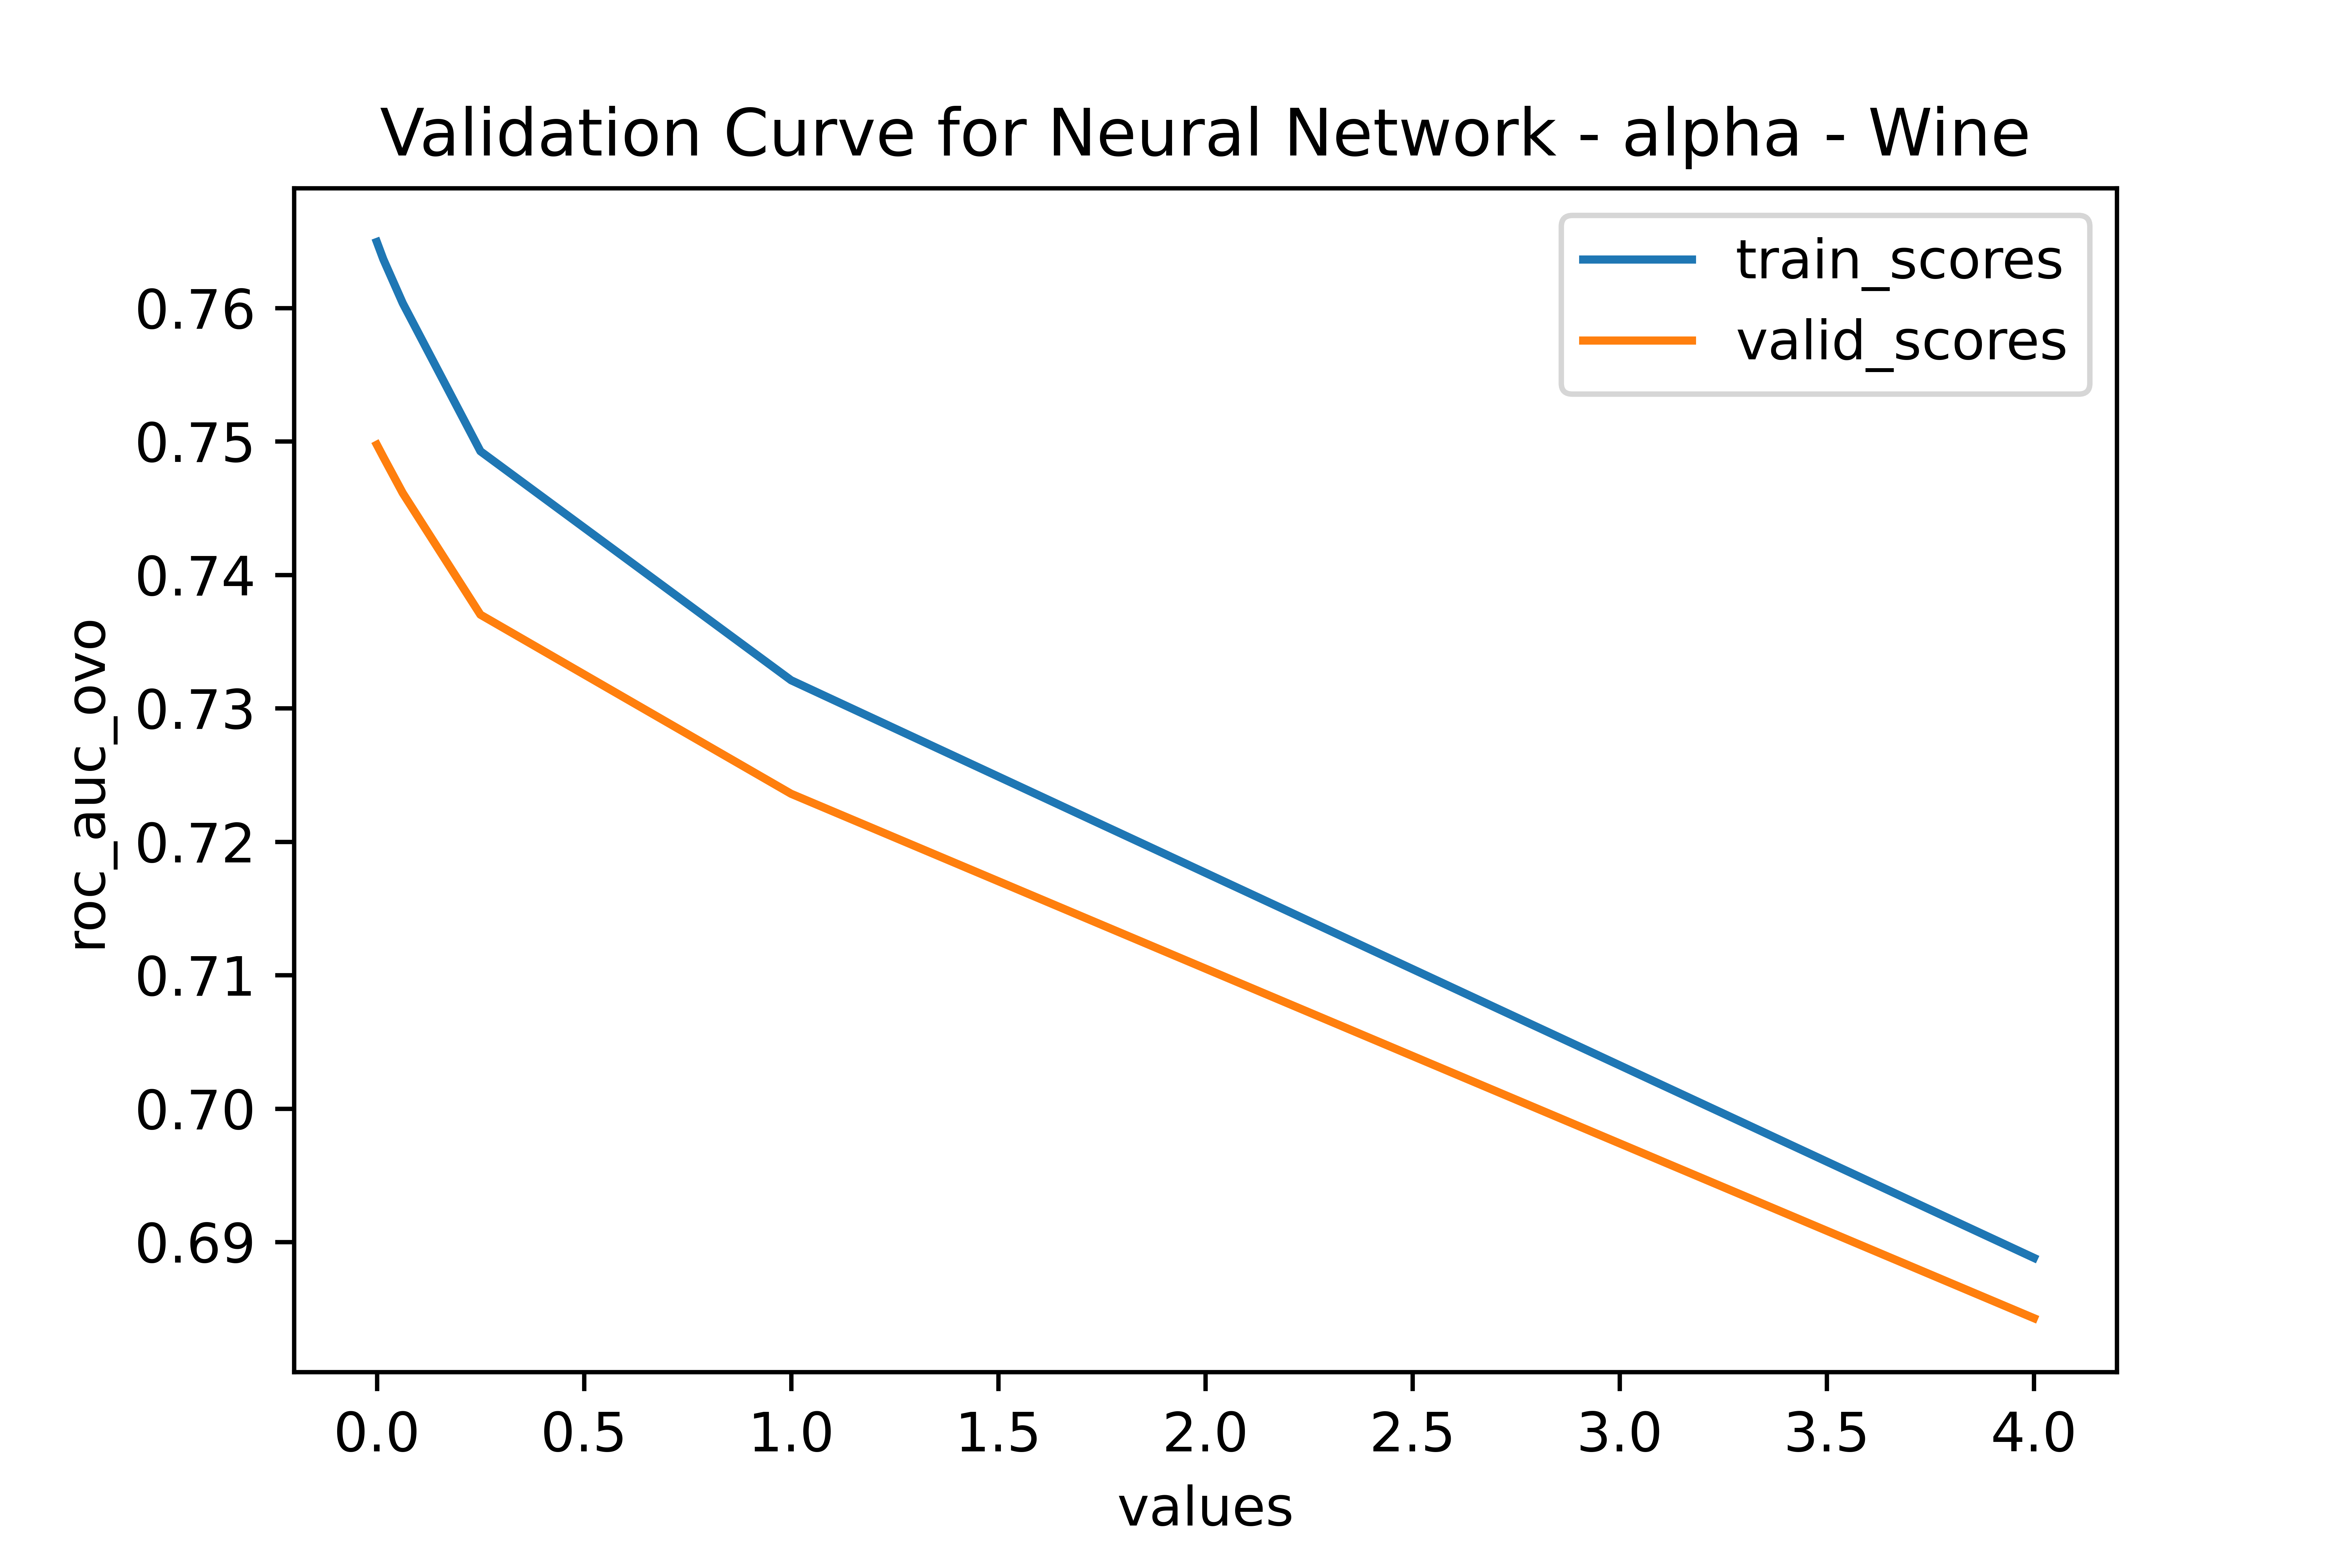
\includegraphics[width=3.4in]{Figures/Wine-0921/NN/val_curve_0.png}
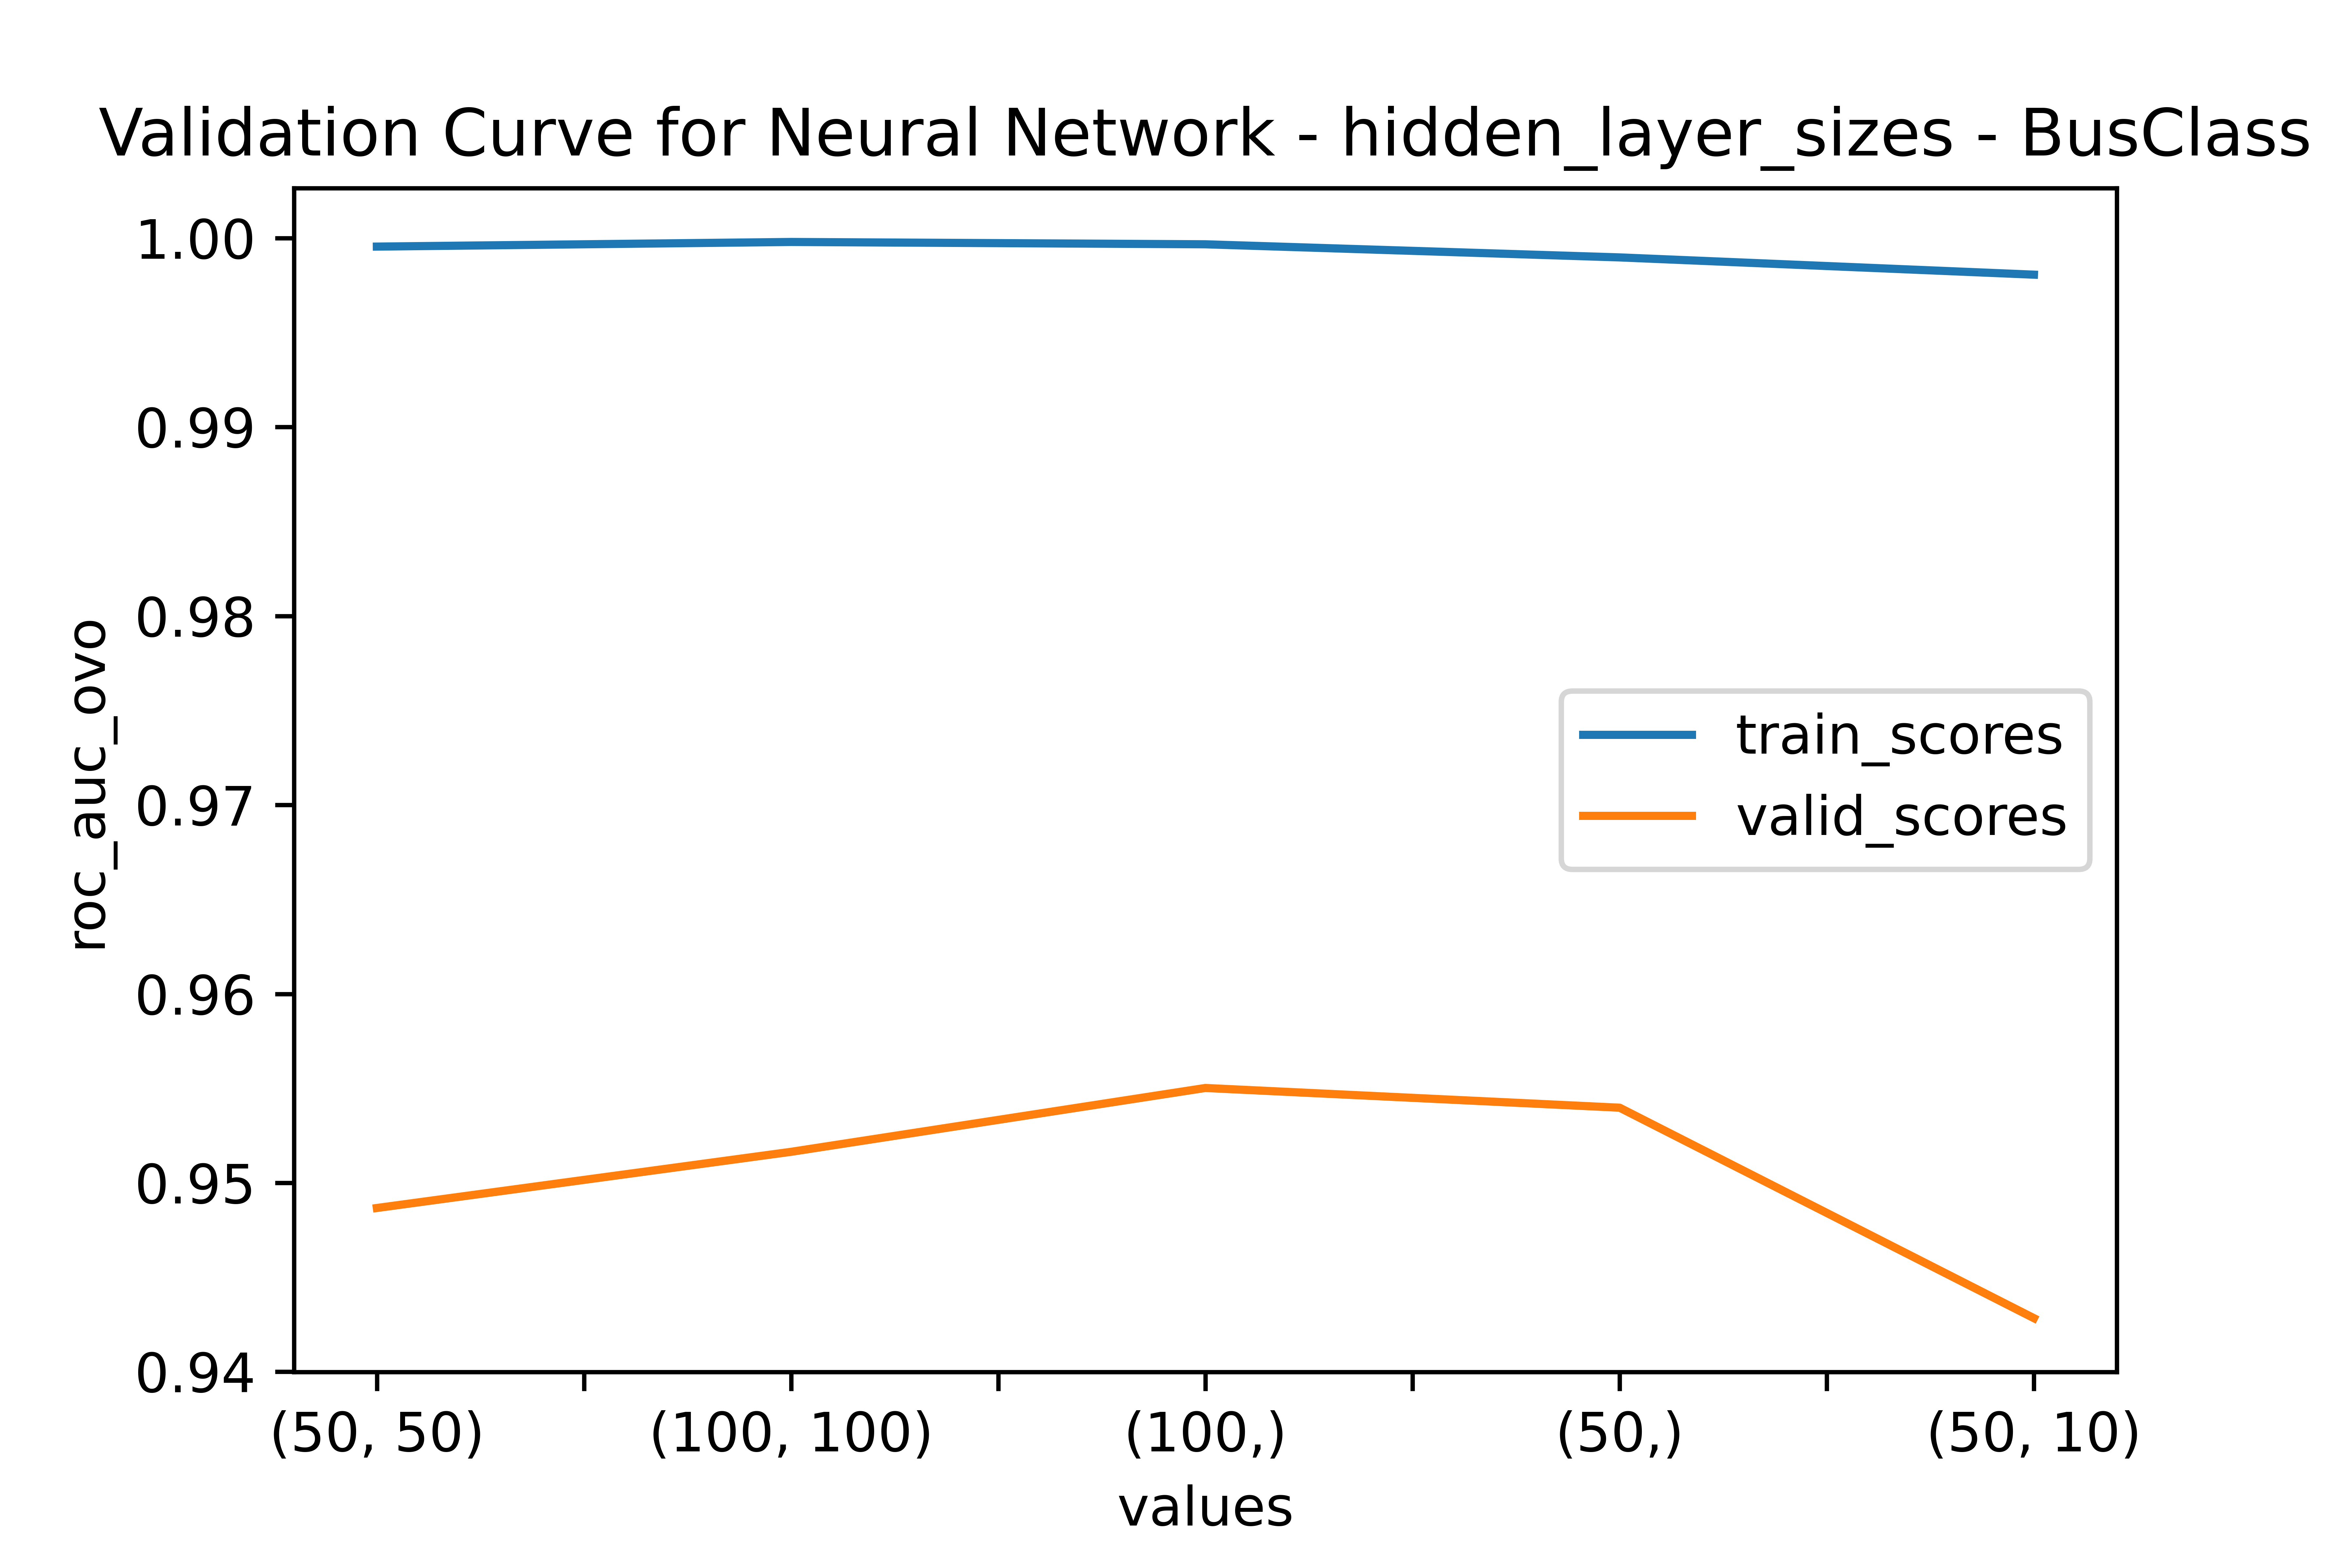
\includegraphics[width=3.4in]{Figures/BusClass-0920/NN/val_curve_1.png}
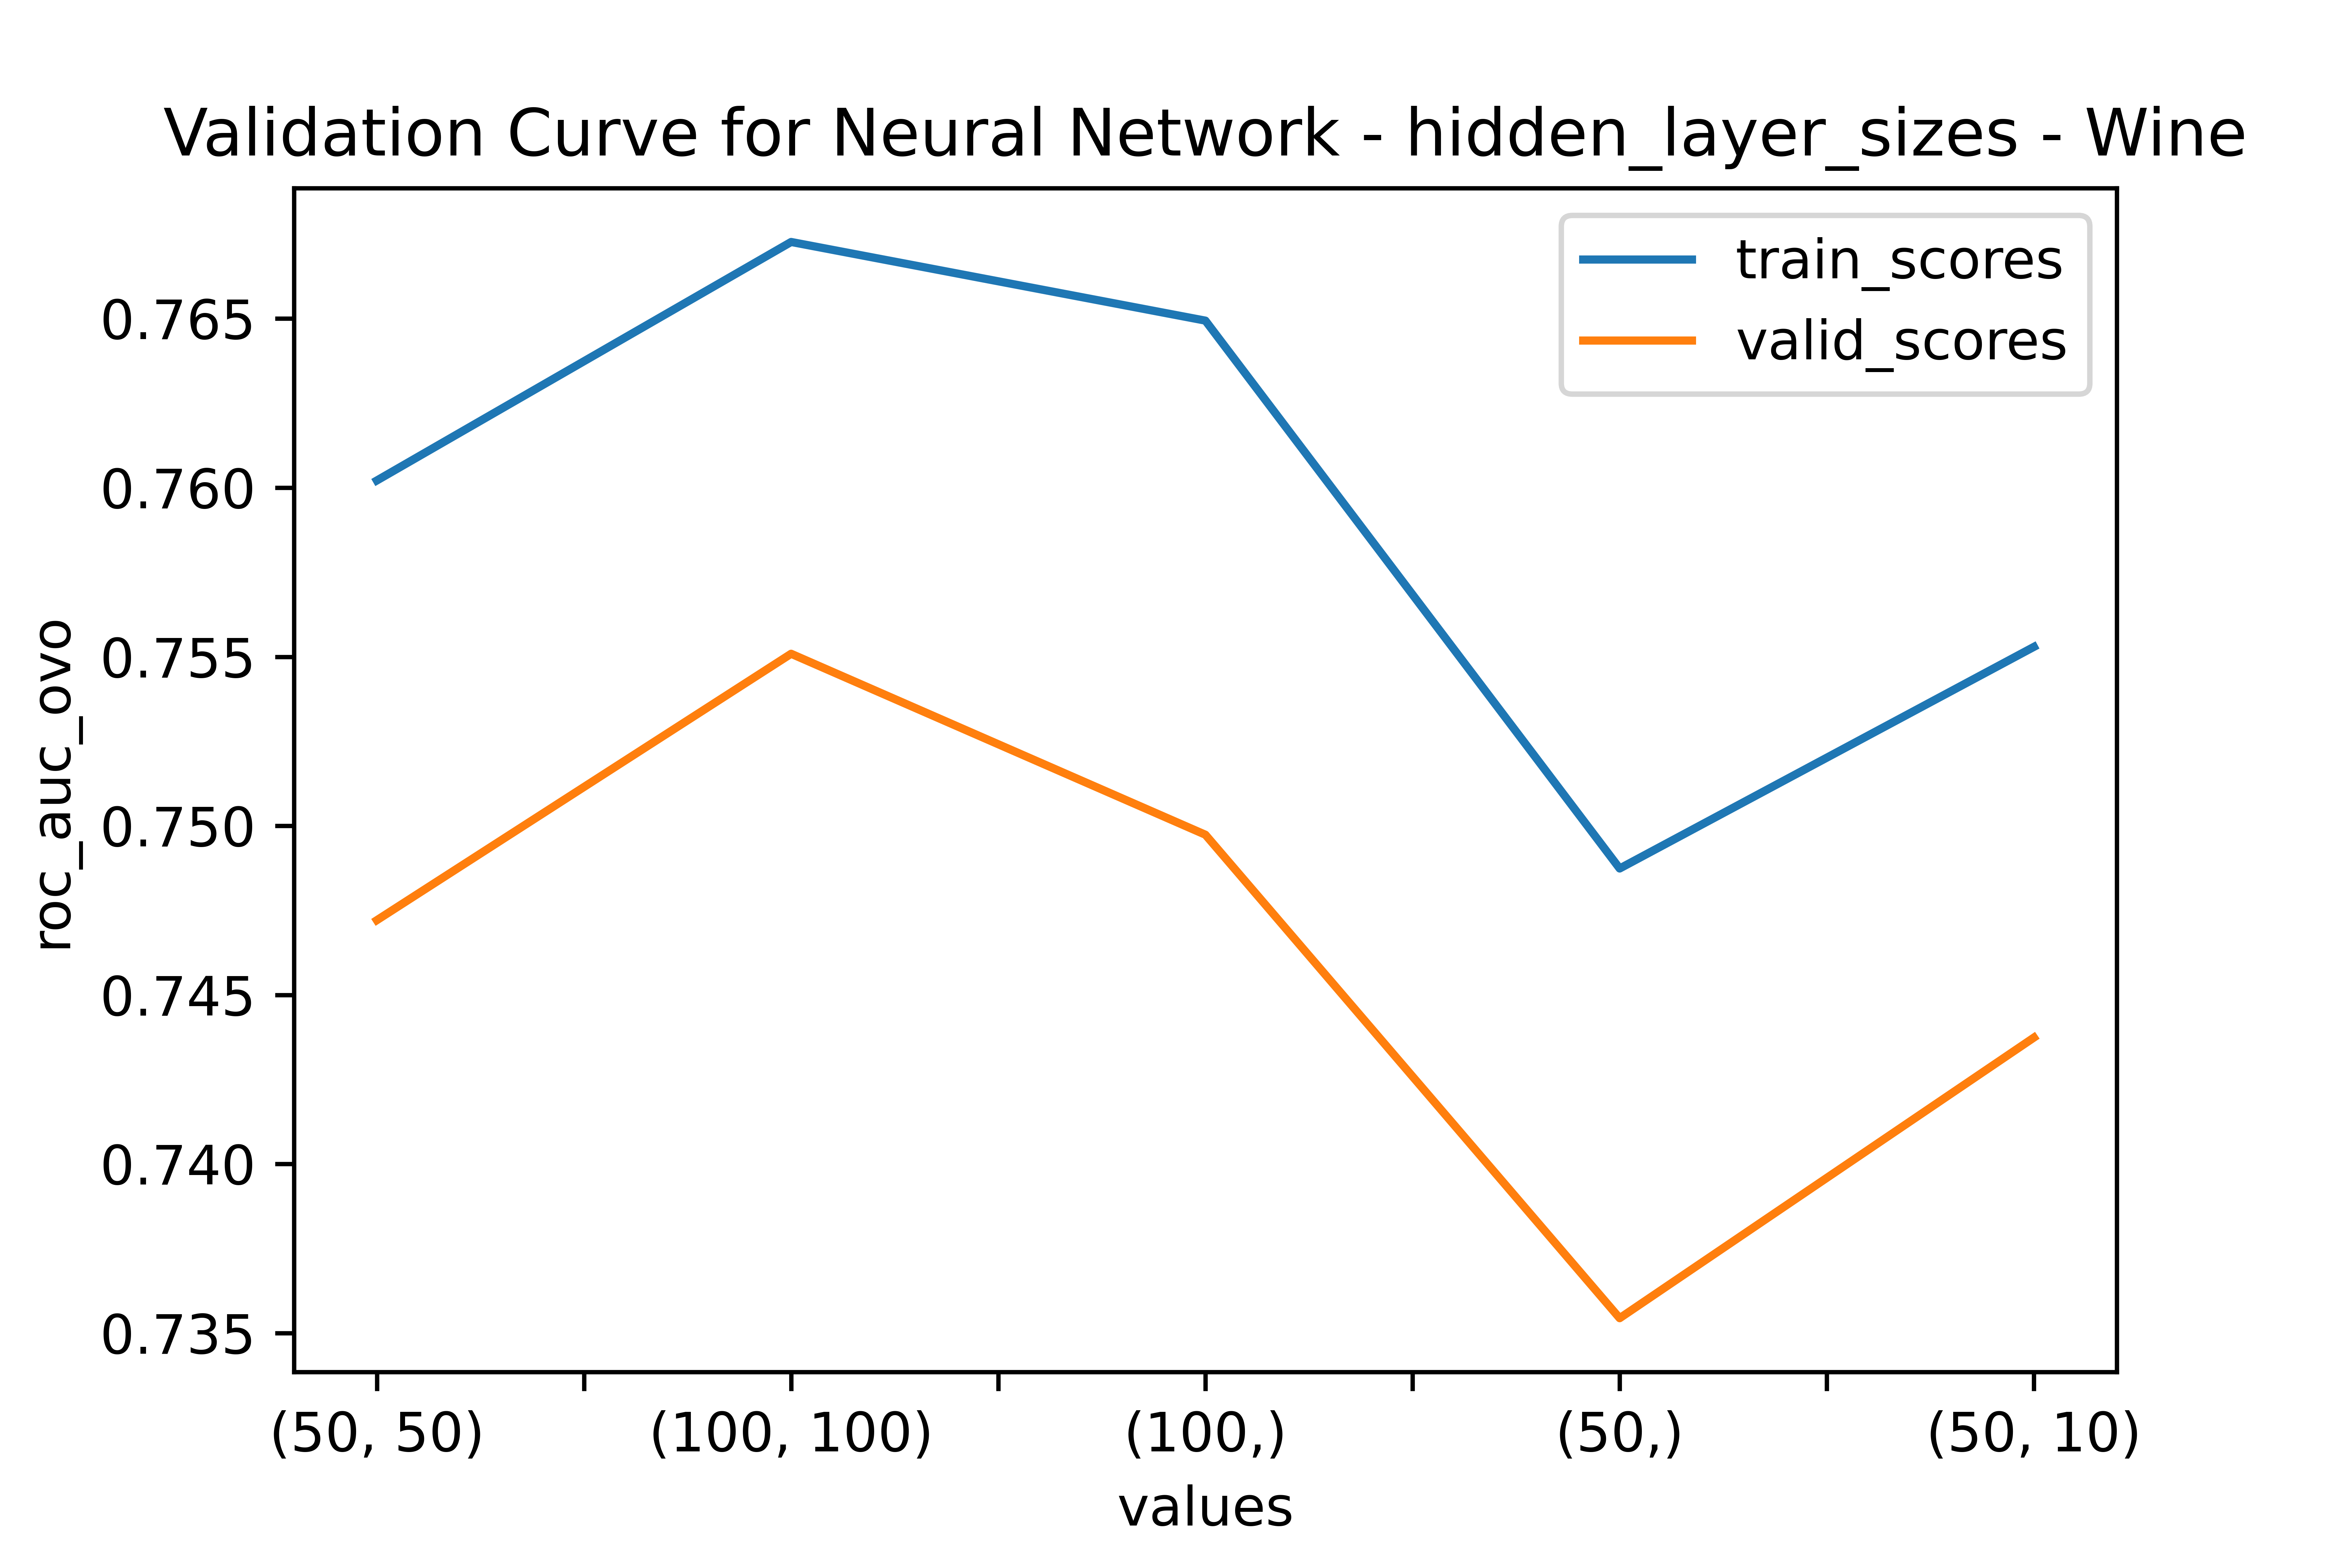
\includegraphics[width=3.4in]{Figures/Wine-0921/NN/val_curve_1.png}

\subsubsection{Iterative Curves}
It would be beneficial to validate that the neural networks are capturing signal in the training datasets themselves and that they're converging. The iterative plots below help us validate this by proving that the internal loss metric used when training the models is plateauing as the algorithm iterates.

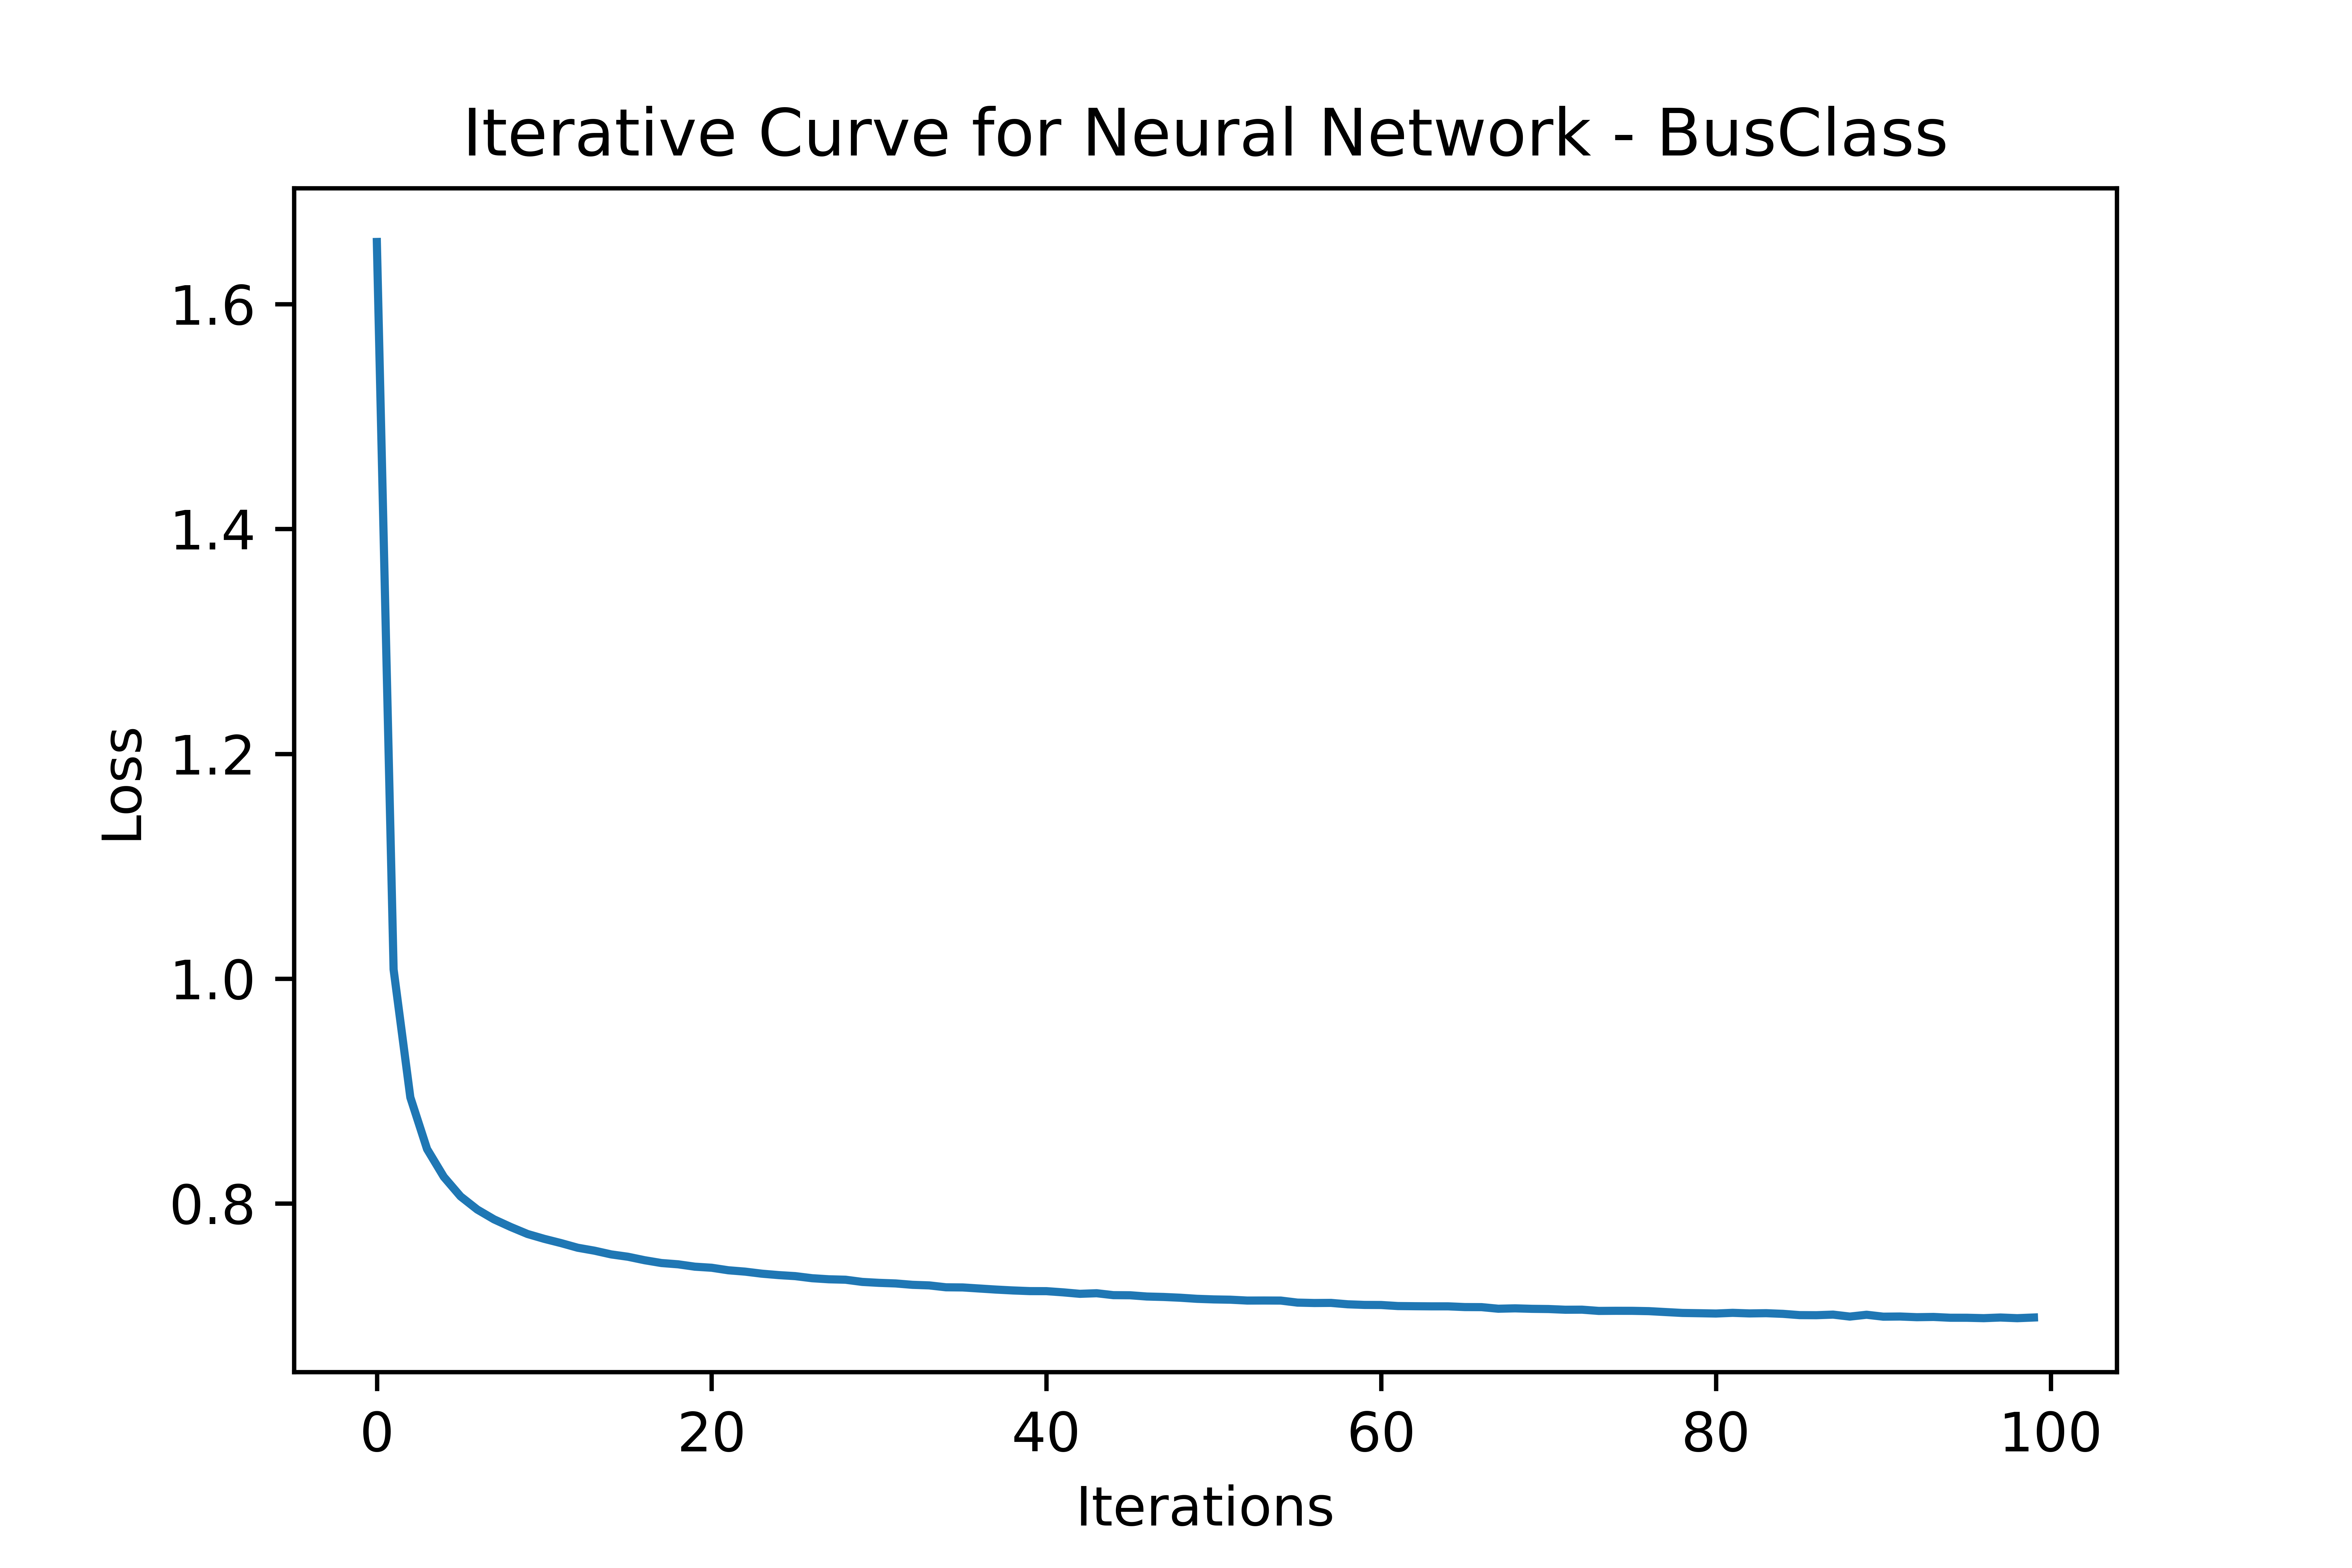
\includegraphics[width=3.4in]{Figures/BusClass-0920/NN/bus_class_iterative_curve.png}
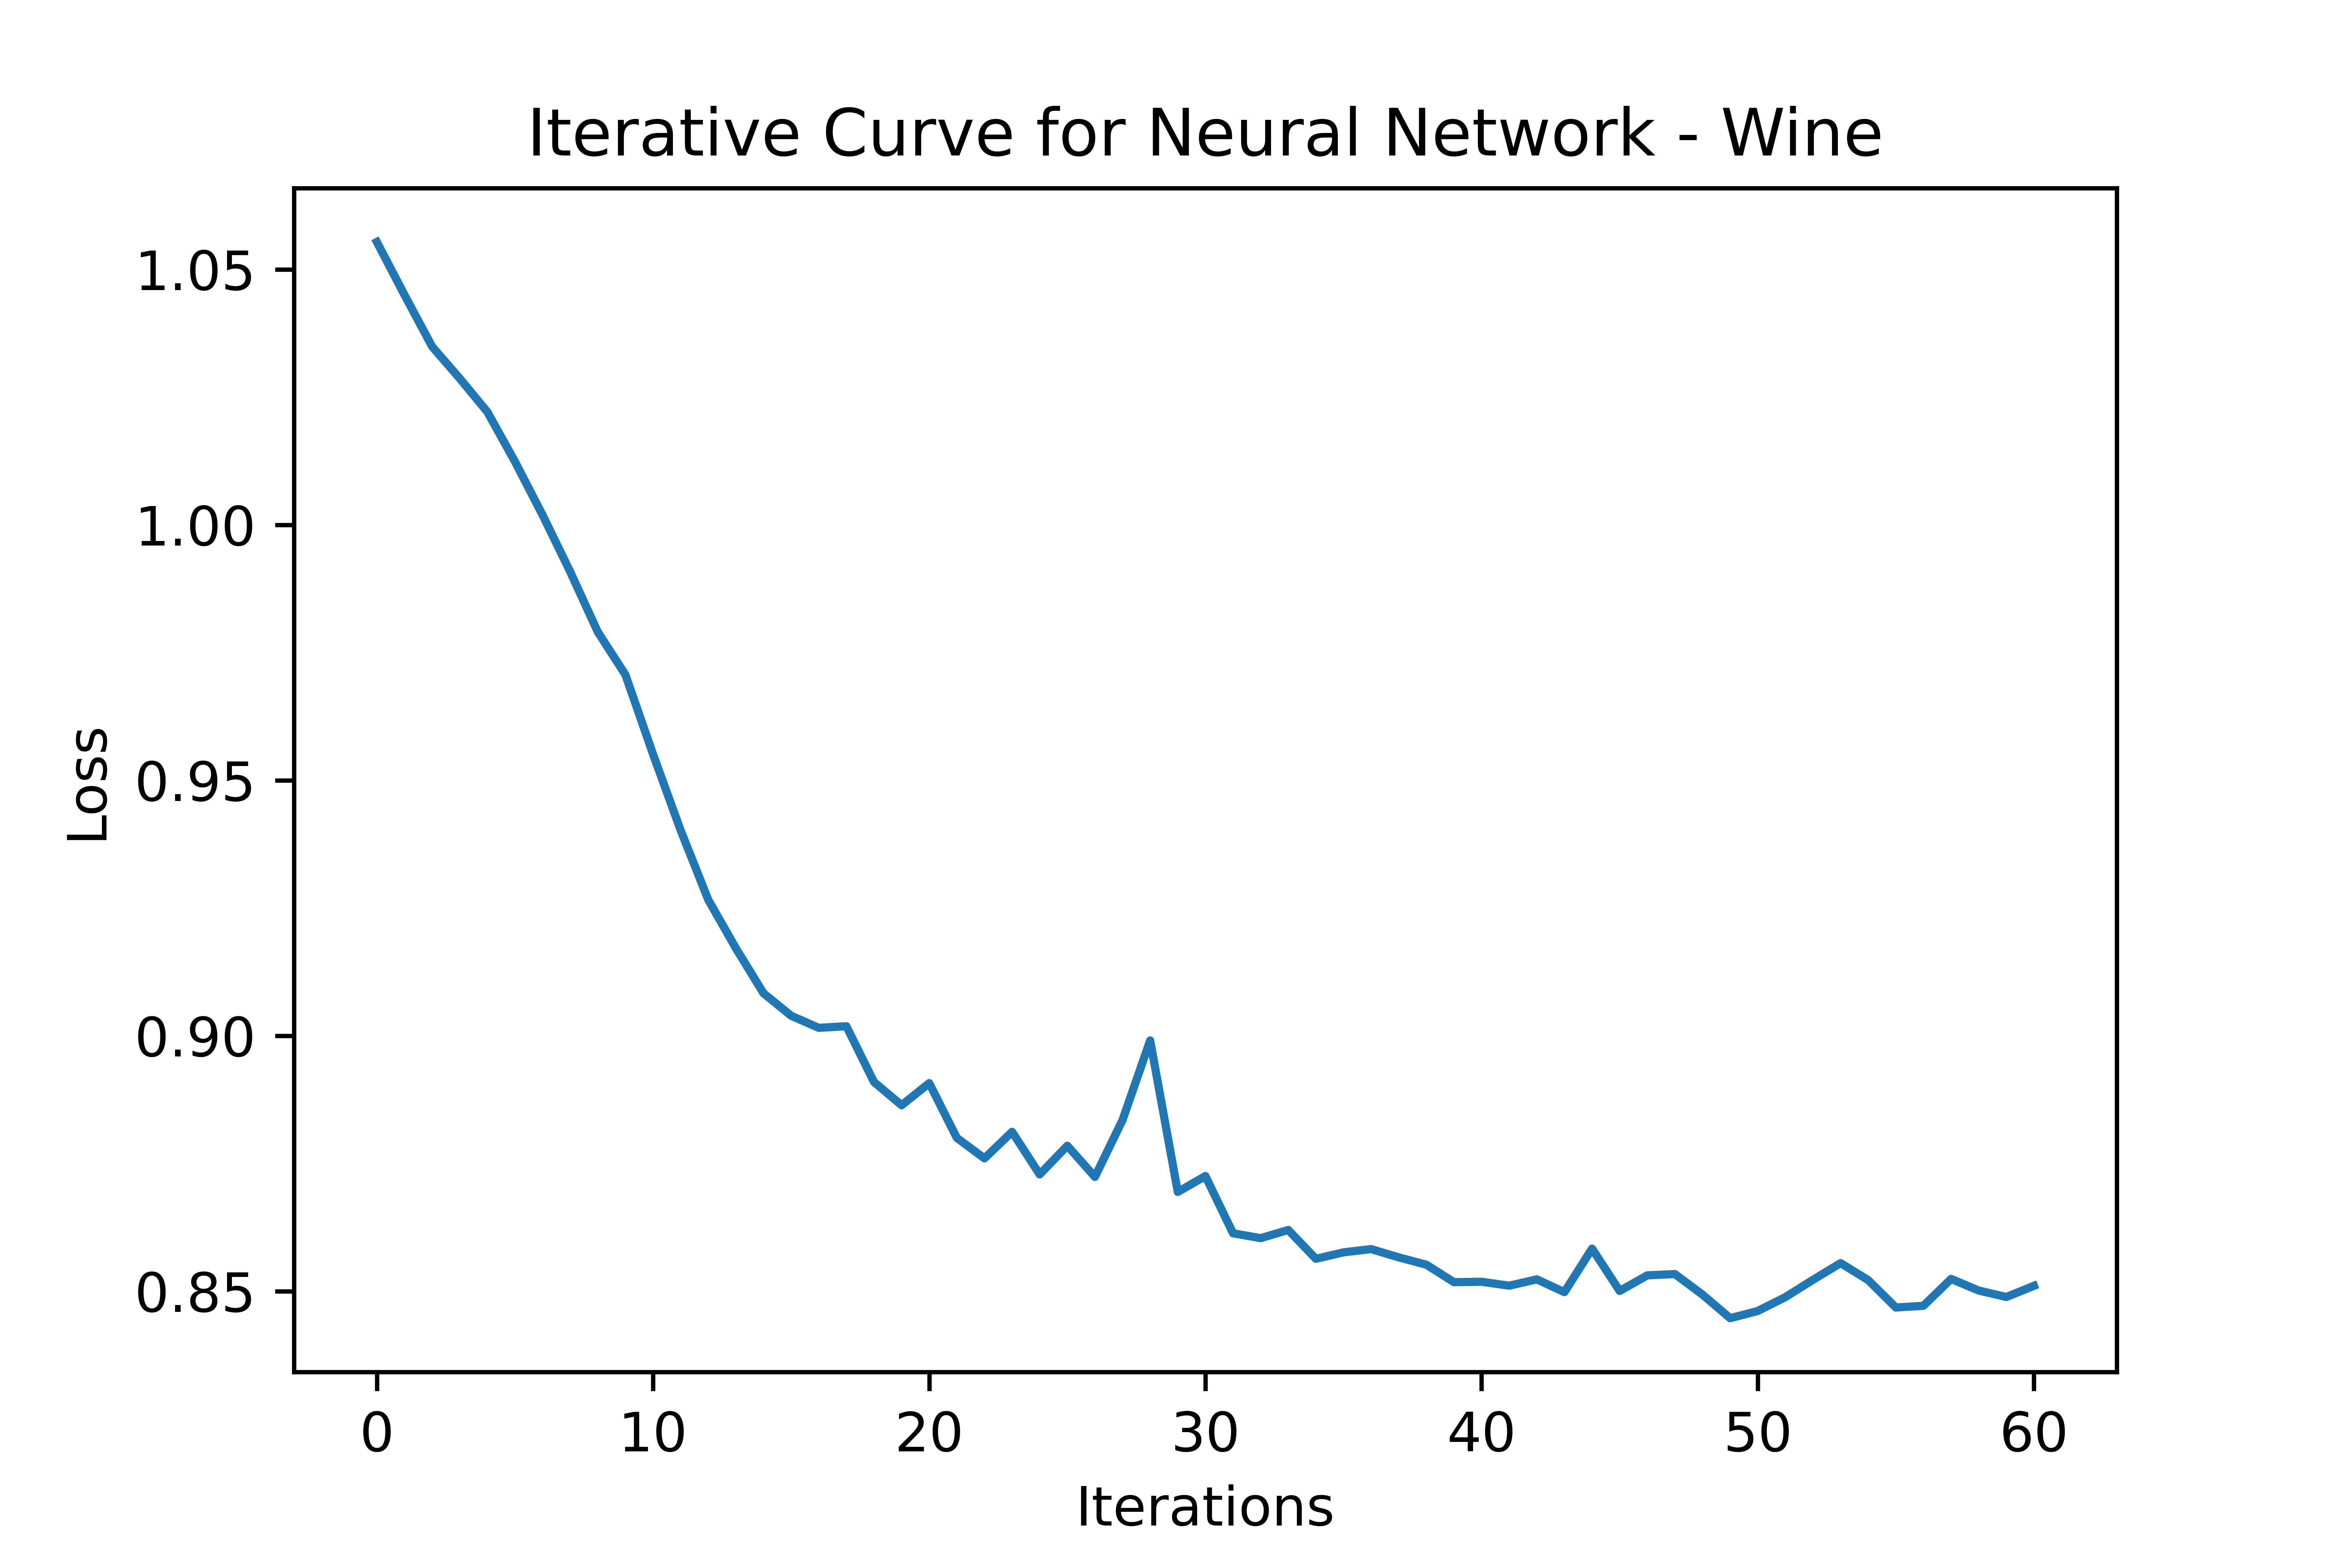
\includegraphics[width=3.4in]{Figures/Wine-0921/NN/wine_iterative_curve.png}

\subsubsection{Learning Curves}
We see an encouraging pattern in the learning curves for the neural network on the business classification task where validation performance is still increasing as a function of training data. This implies that the model is underfit and would benefit from more training data, if we had it. The wine classifier shows a similar but less smooth curve, exhibiting a little more "leveling out" than its counterpart. This one implies that we are less underfit, though not overfitting.

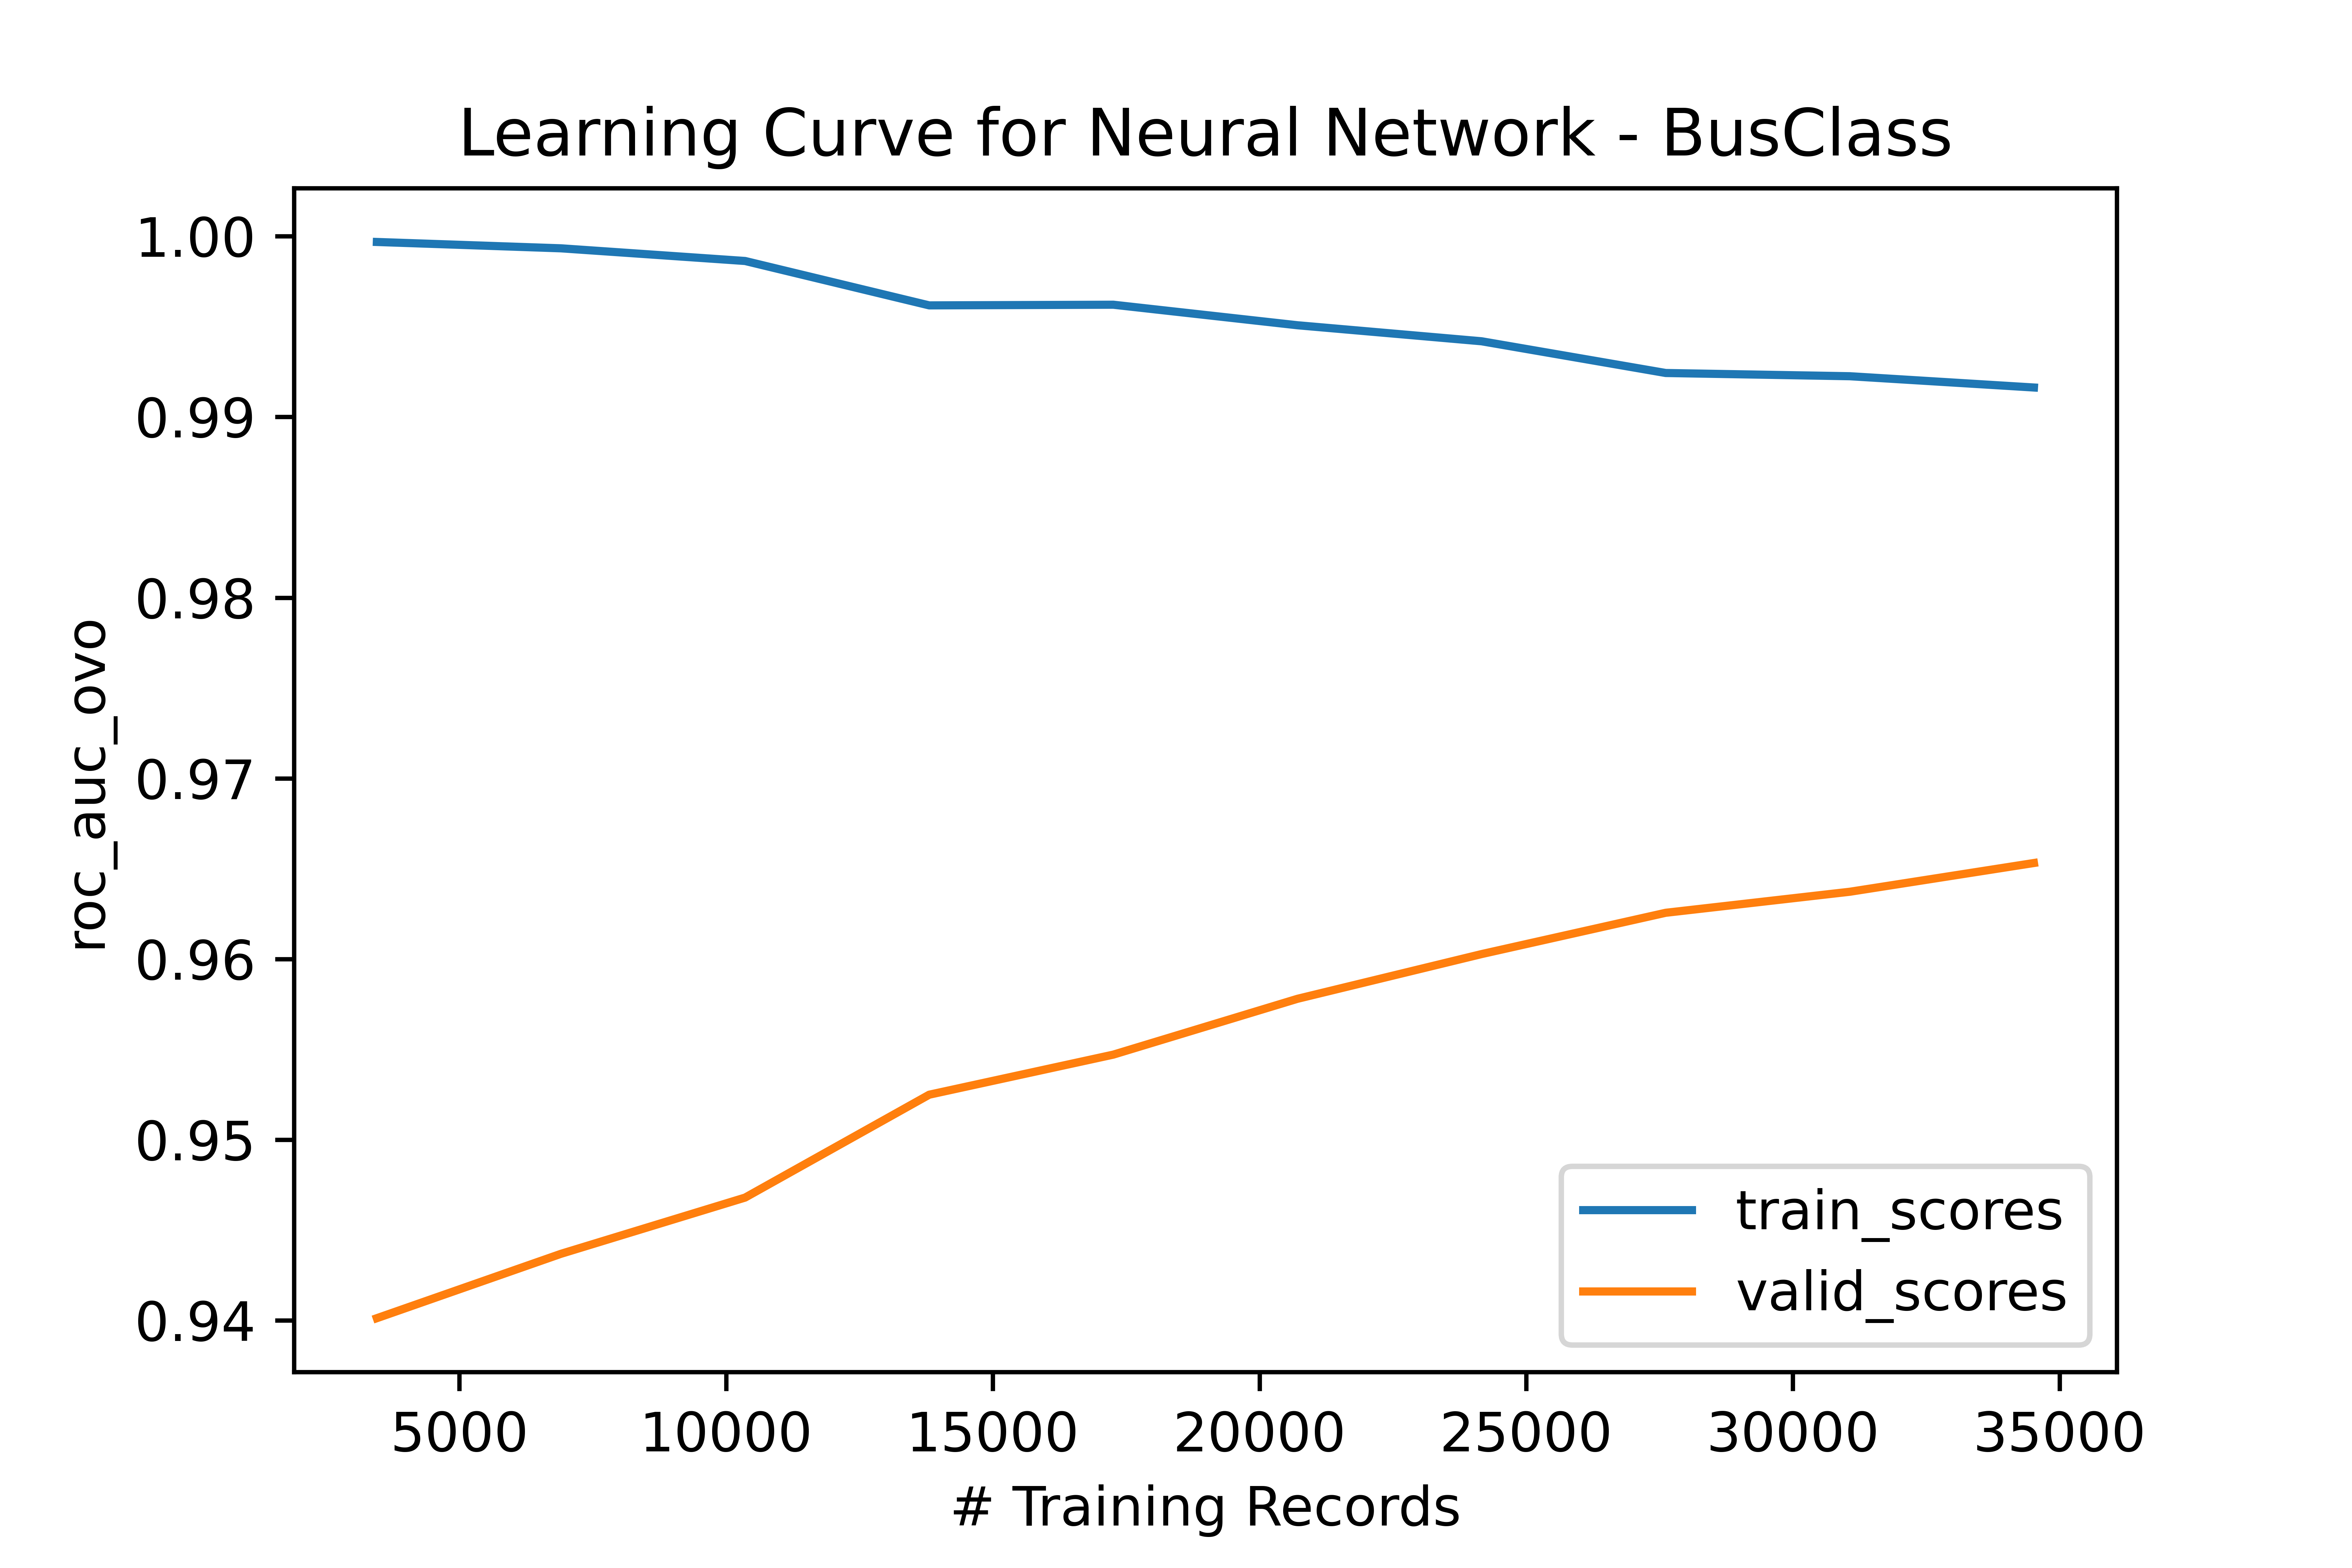
\includegraphics[width=3.4in]{Figures/BusClass-0920/NN/learn_curve.png}
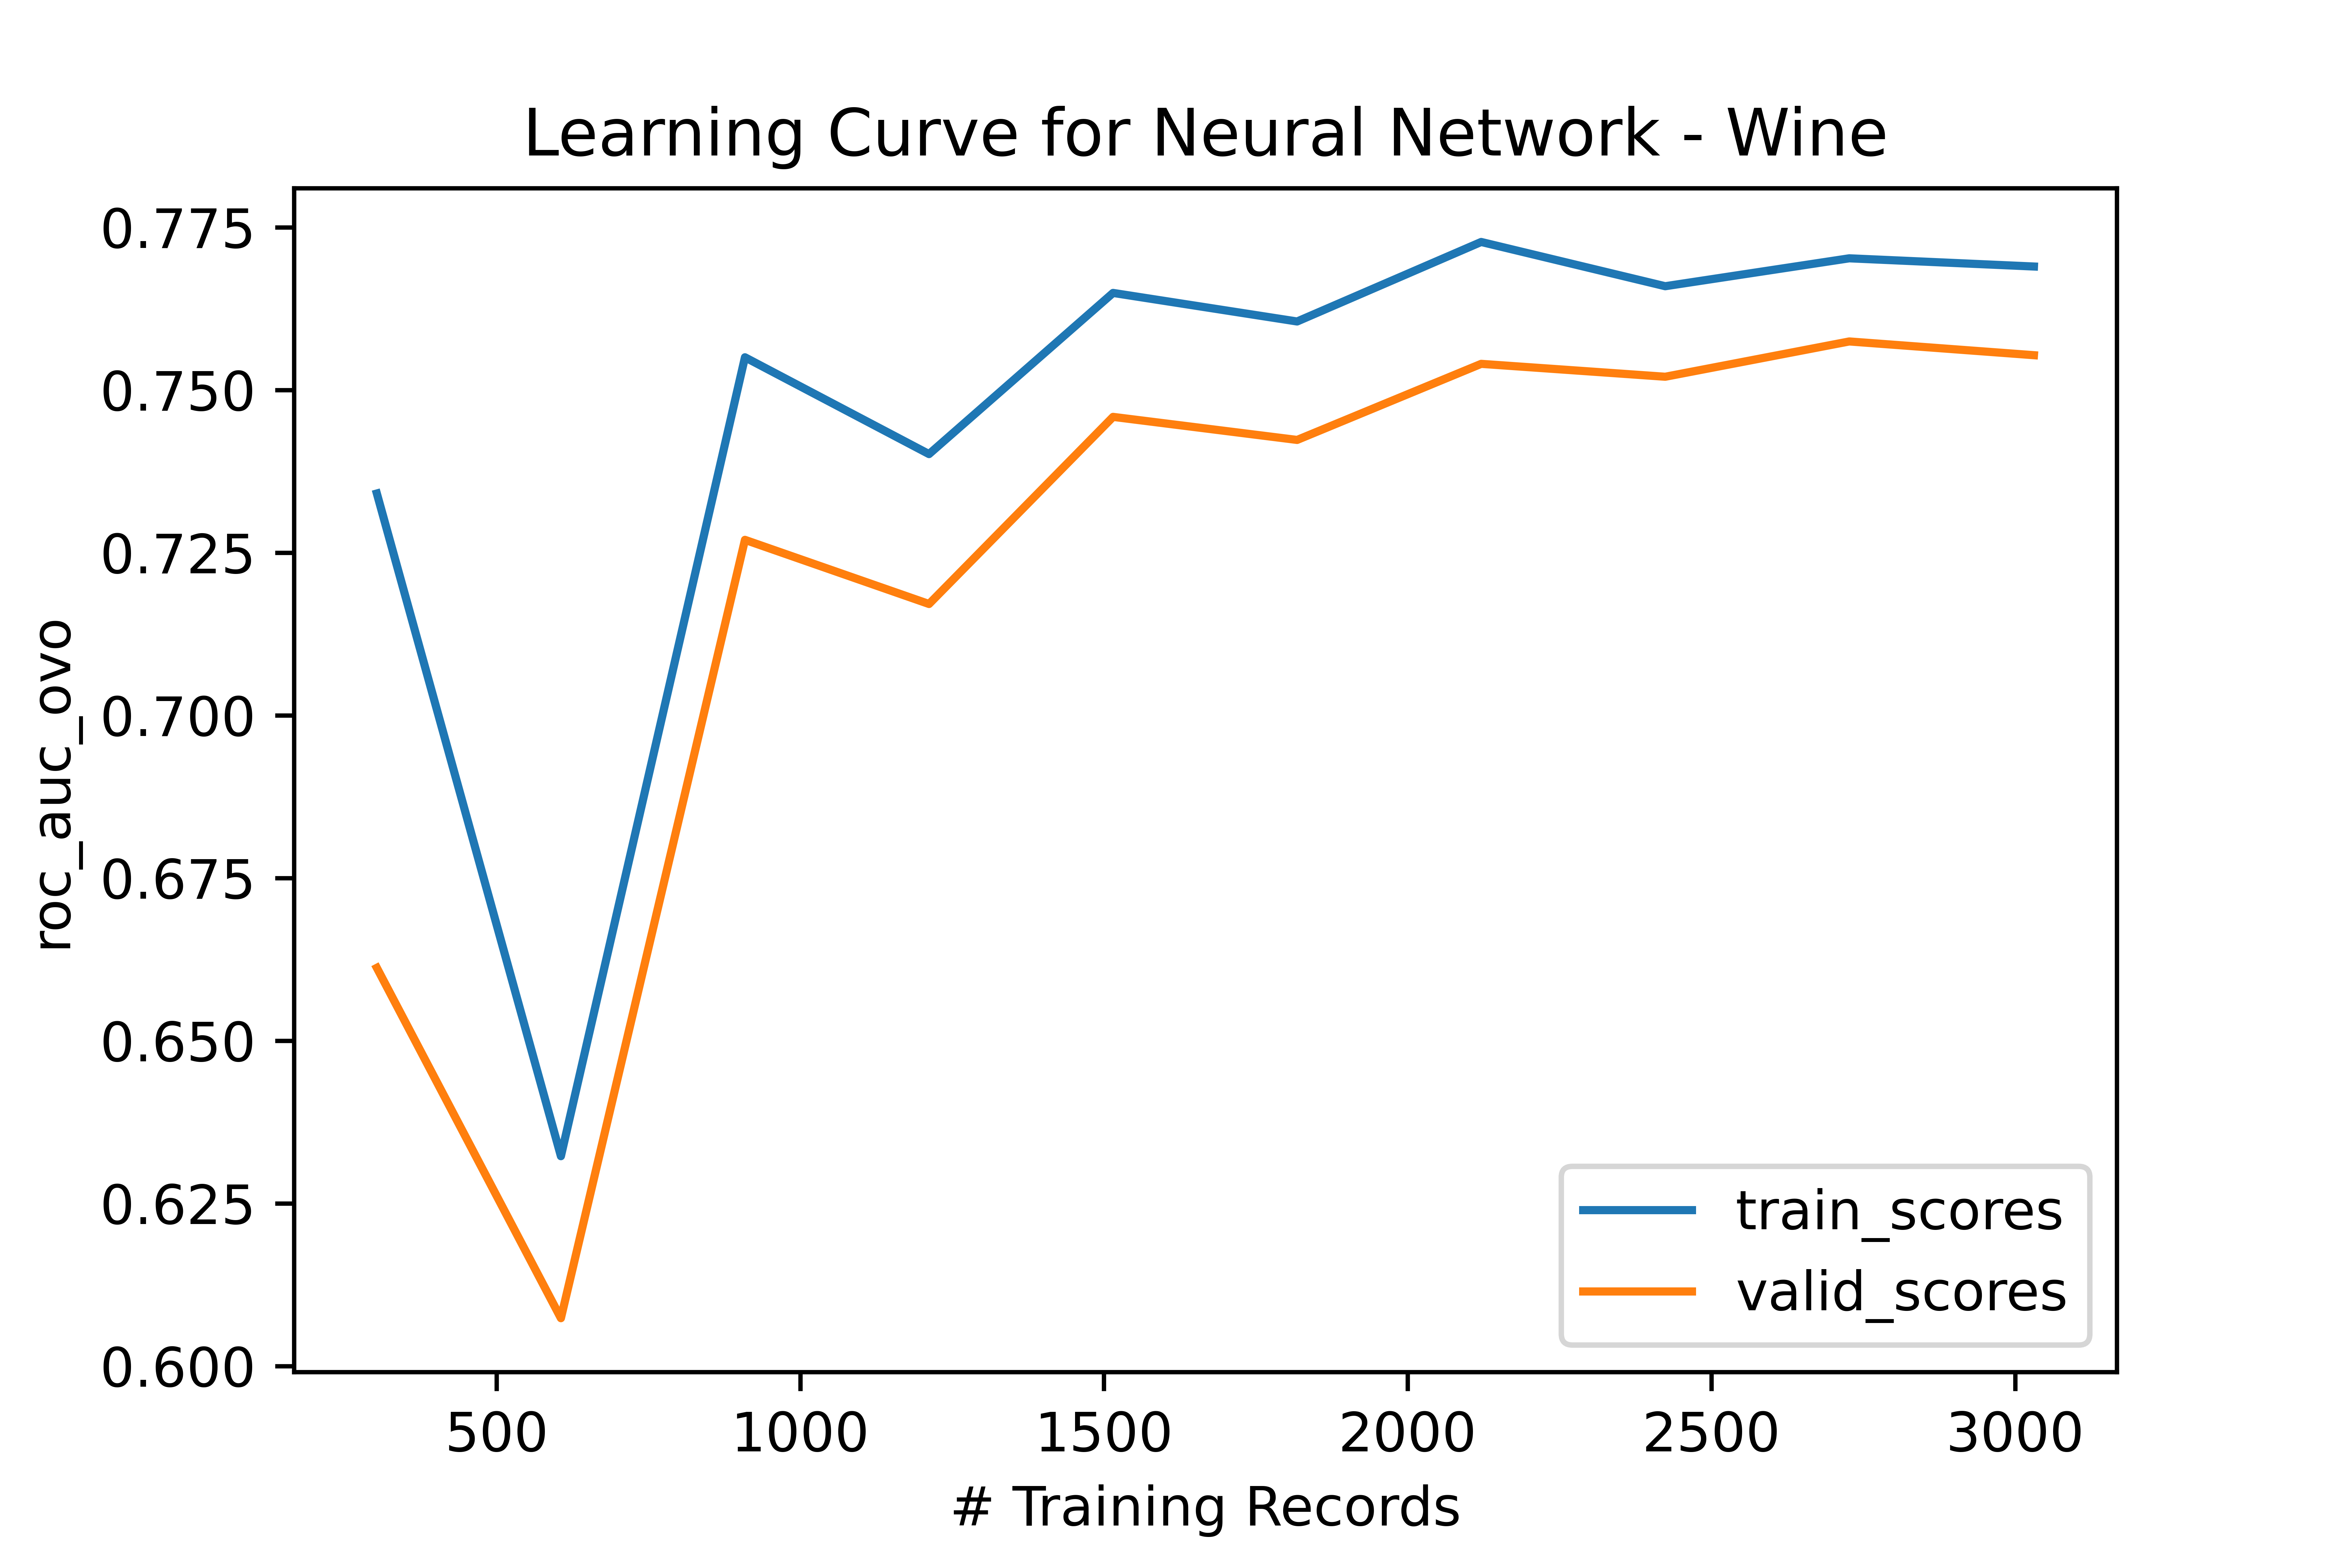
\includegraphics[width=3.4in]{Figures/Wine-0921/NN/learn_curve.png}

\subsubsection{Wall Clock Time}
For the fitting and scoring times, we see a similar pattern of linear fit time and near constant score time. The major difference between the two datasets is just magnitude: the much larger business classification dataset requires more time than the smaller wine dataset.

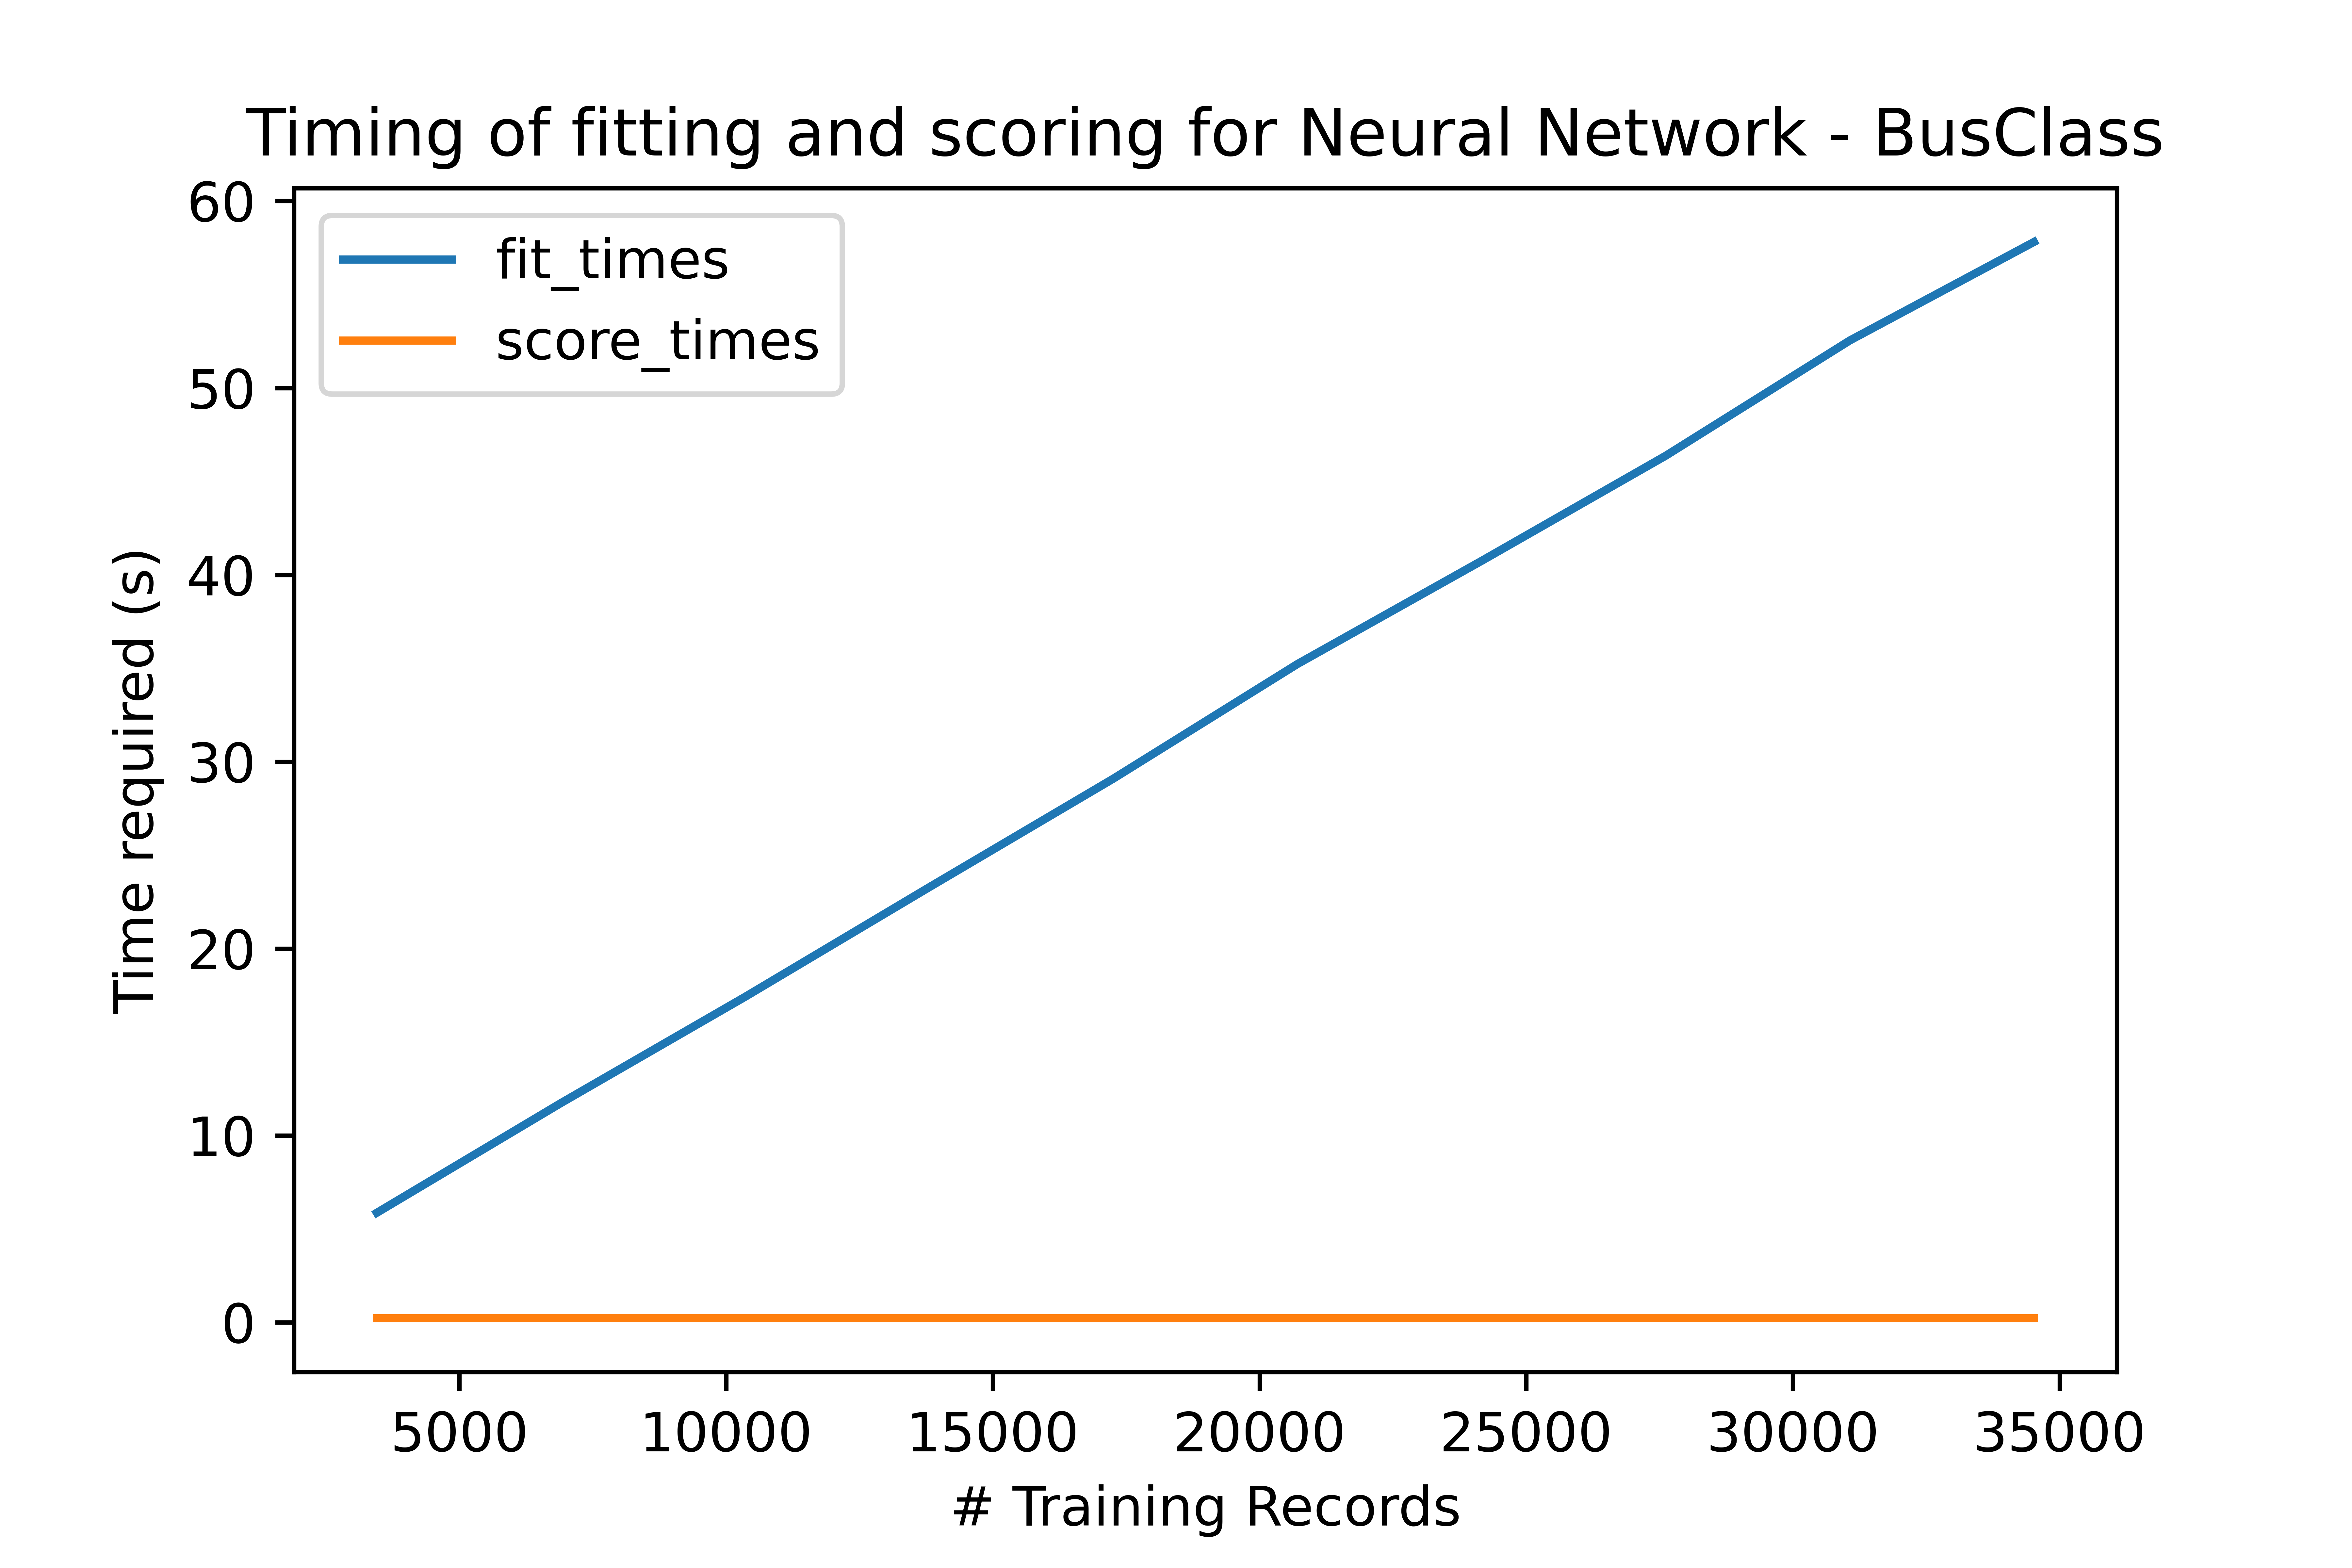
\includegraphics[width=3.4in]{Figures/BusClass-0920/NN/time_curve.png}
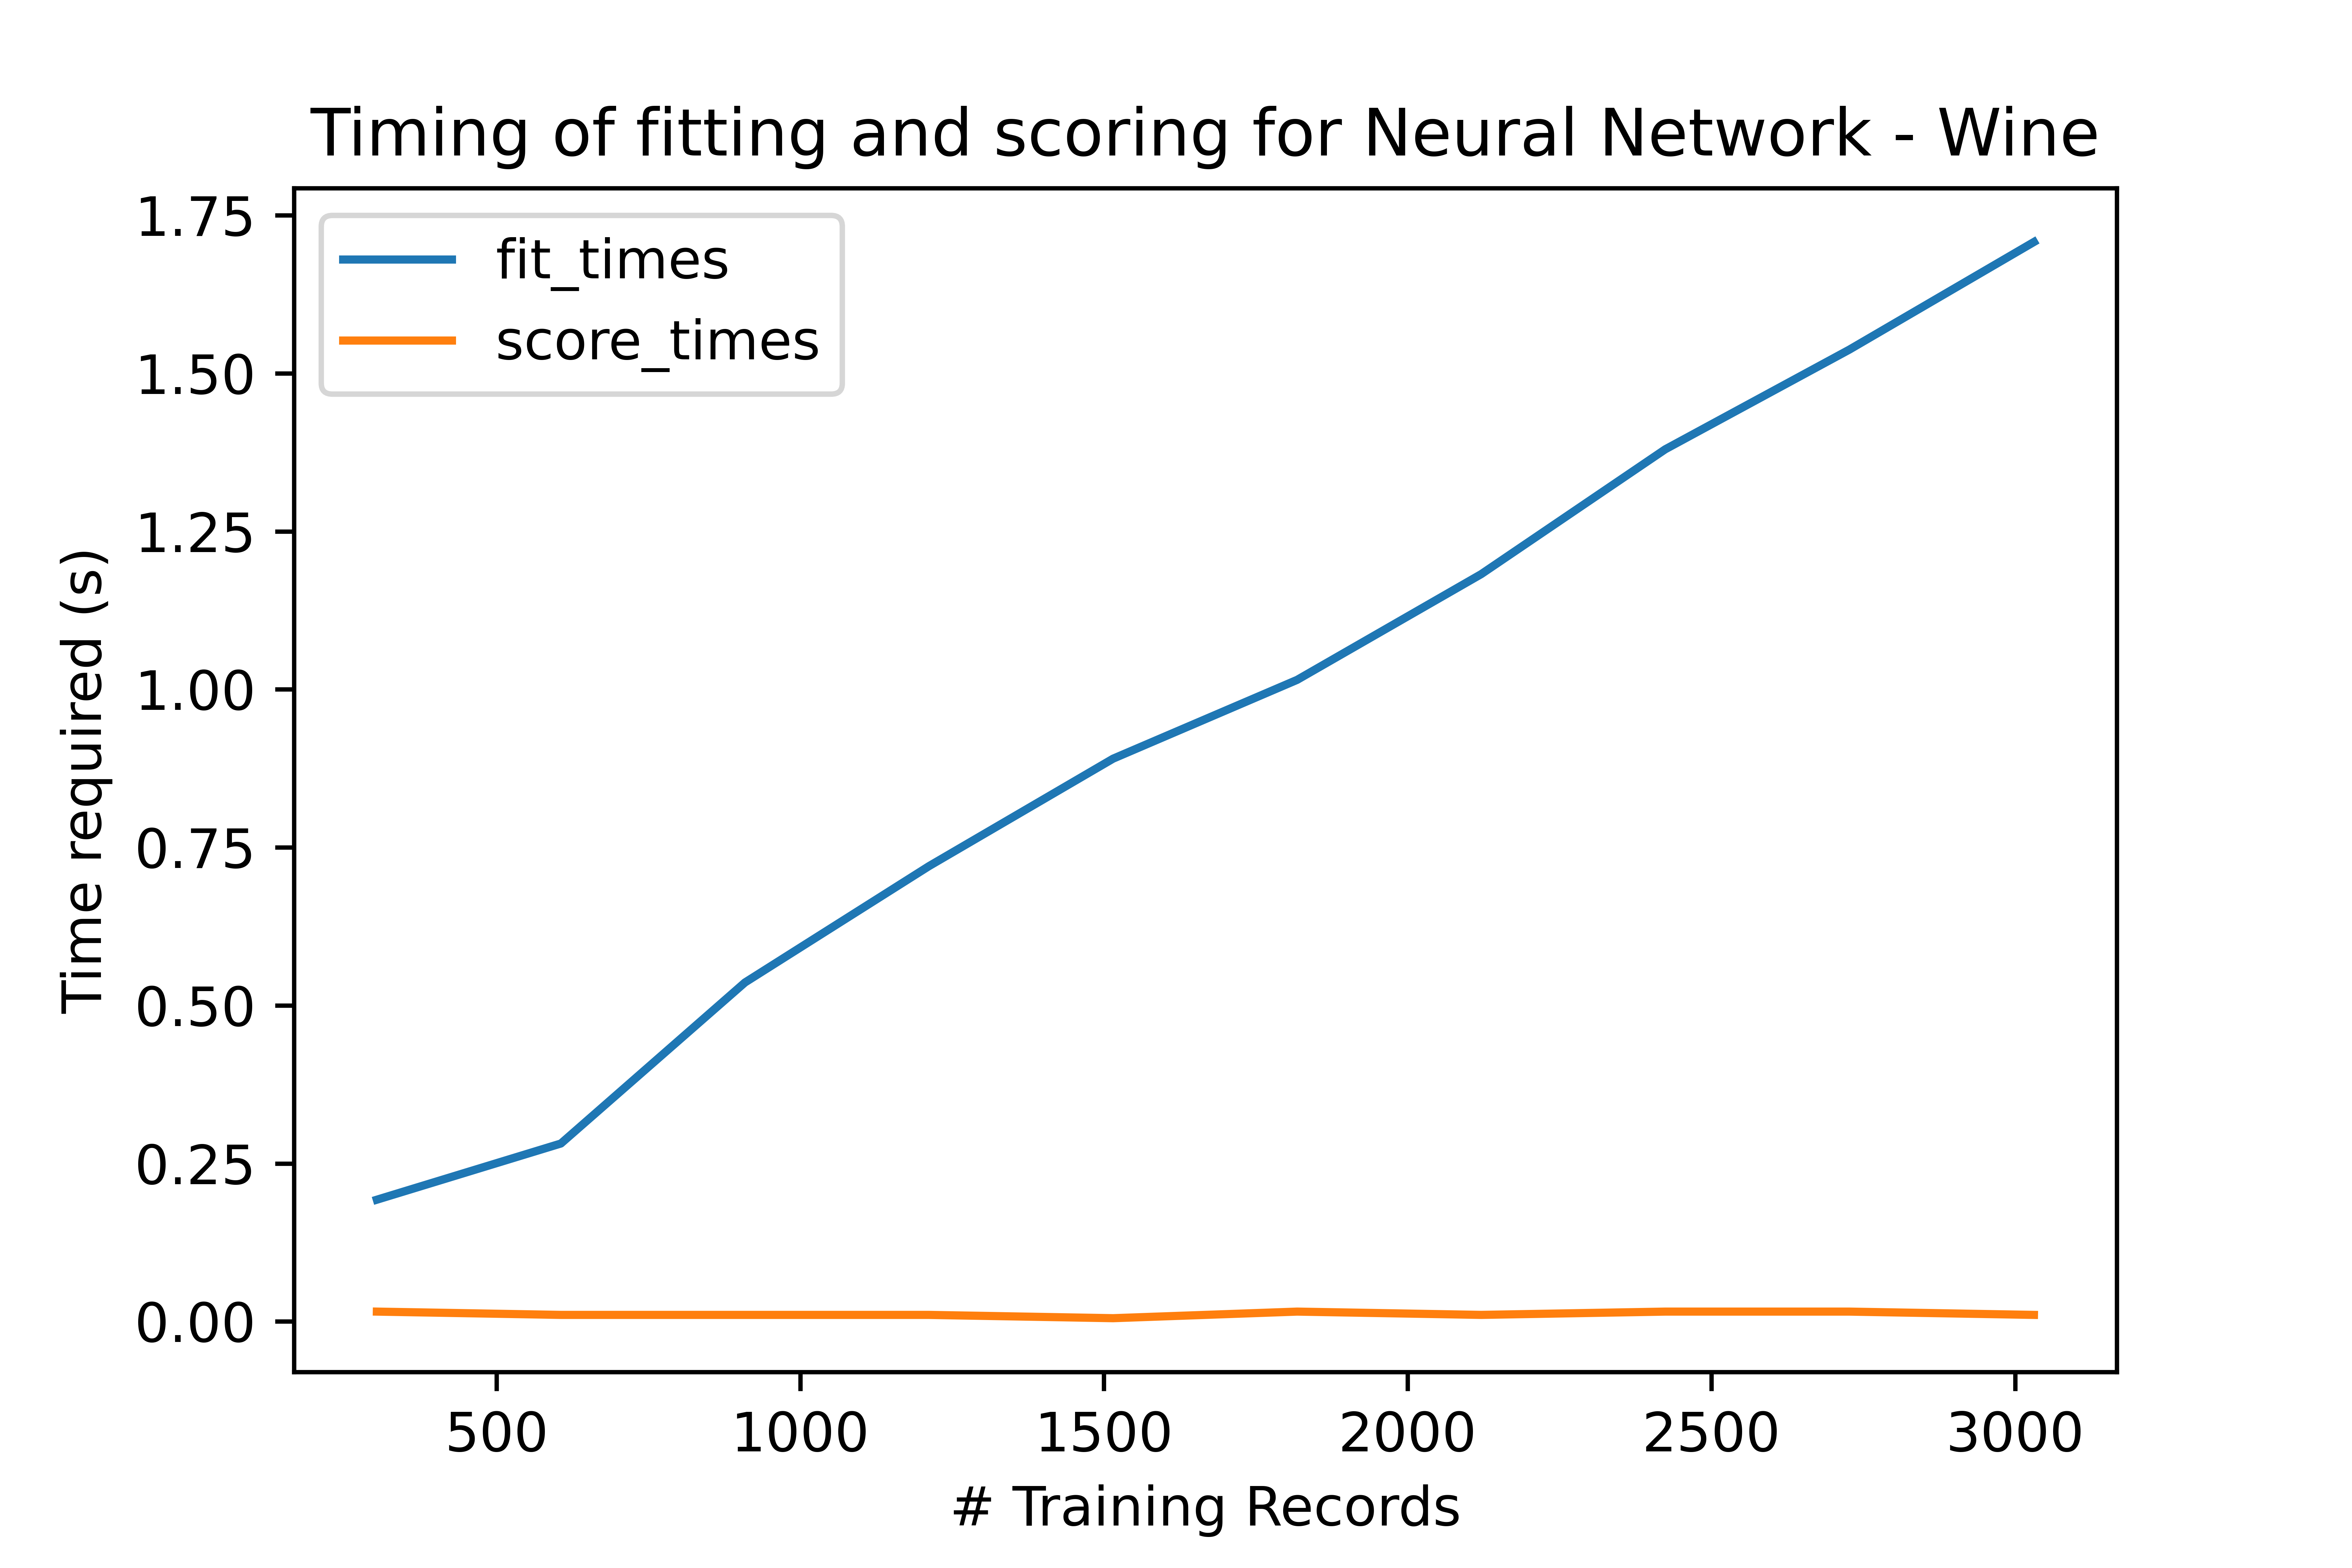
\includegraphics[width=3.4in]{Figures/Wine-0921/NN/time_curve.png}


\subsection{Boosting}

\subsubsection{Hyperparameter Tuning}
True to the claims in the lecture videos, the boosting technique seems to be highly robust to overfitting. Even with a fairly high learning rate of 0.05, increasing the number of estimators from 1,000 to 10,000 had hardly any impact on performance on the validation set, even as the performance on the training set increased. Once again, we saw that little to no pruning was optimal for these algorithms.

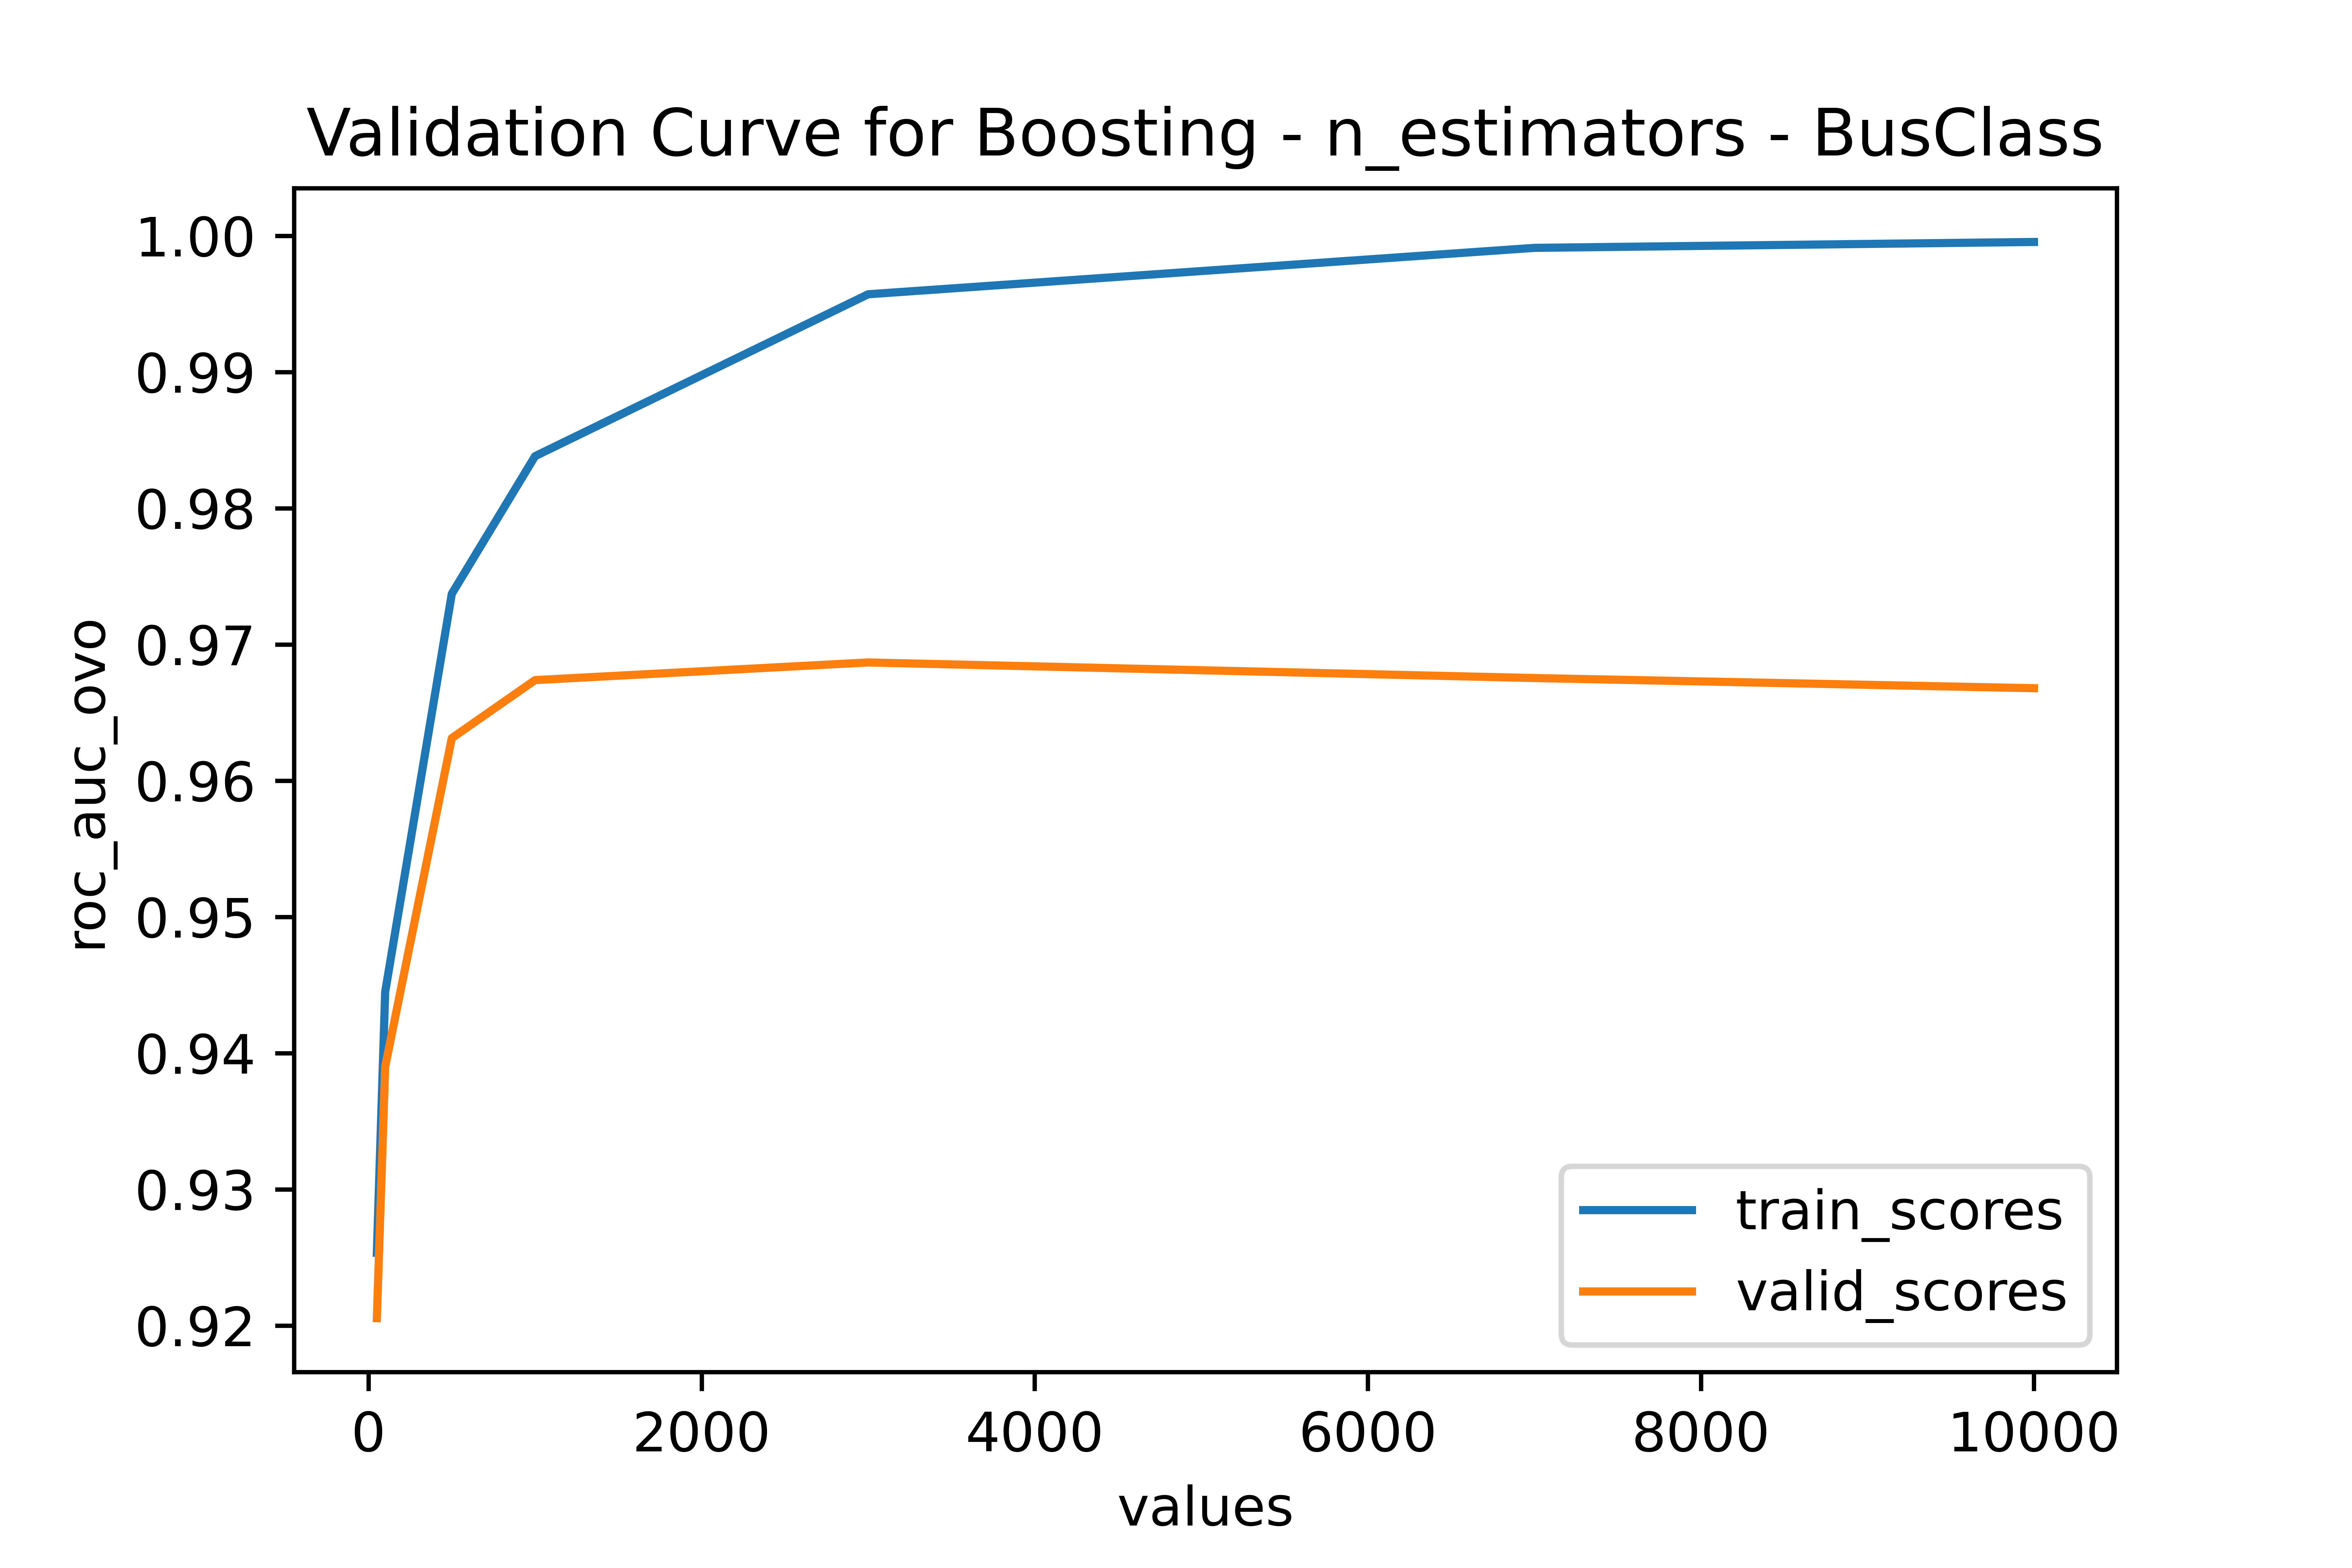
\includegraphics[width=3.4in]{Figures/BusClass-0920/GBM/val_curve_0.png}
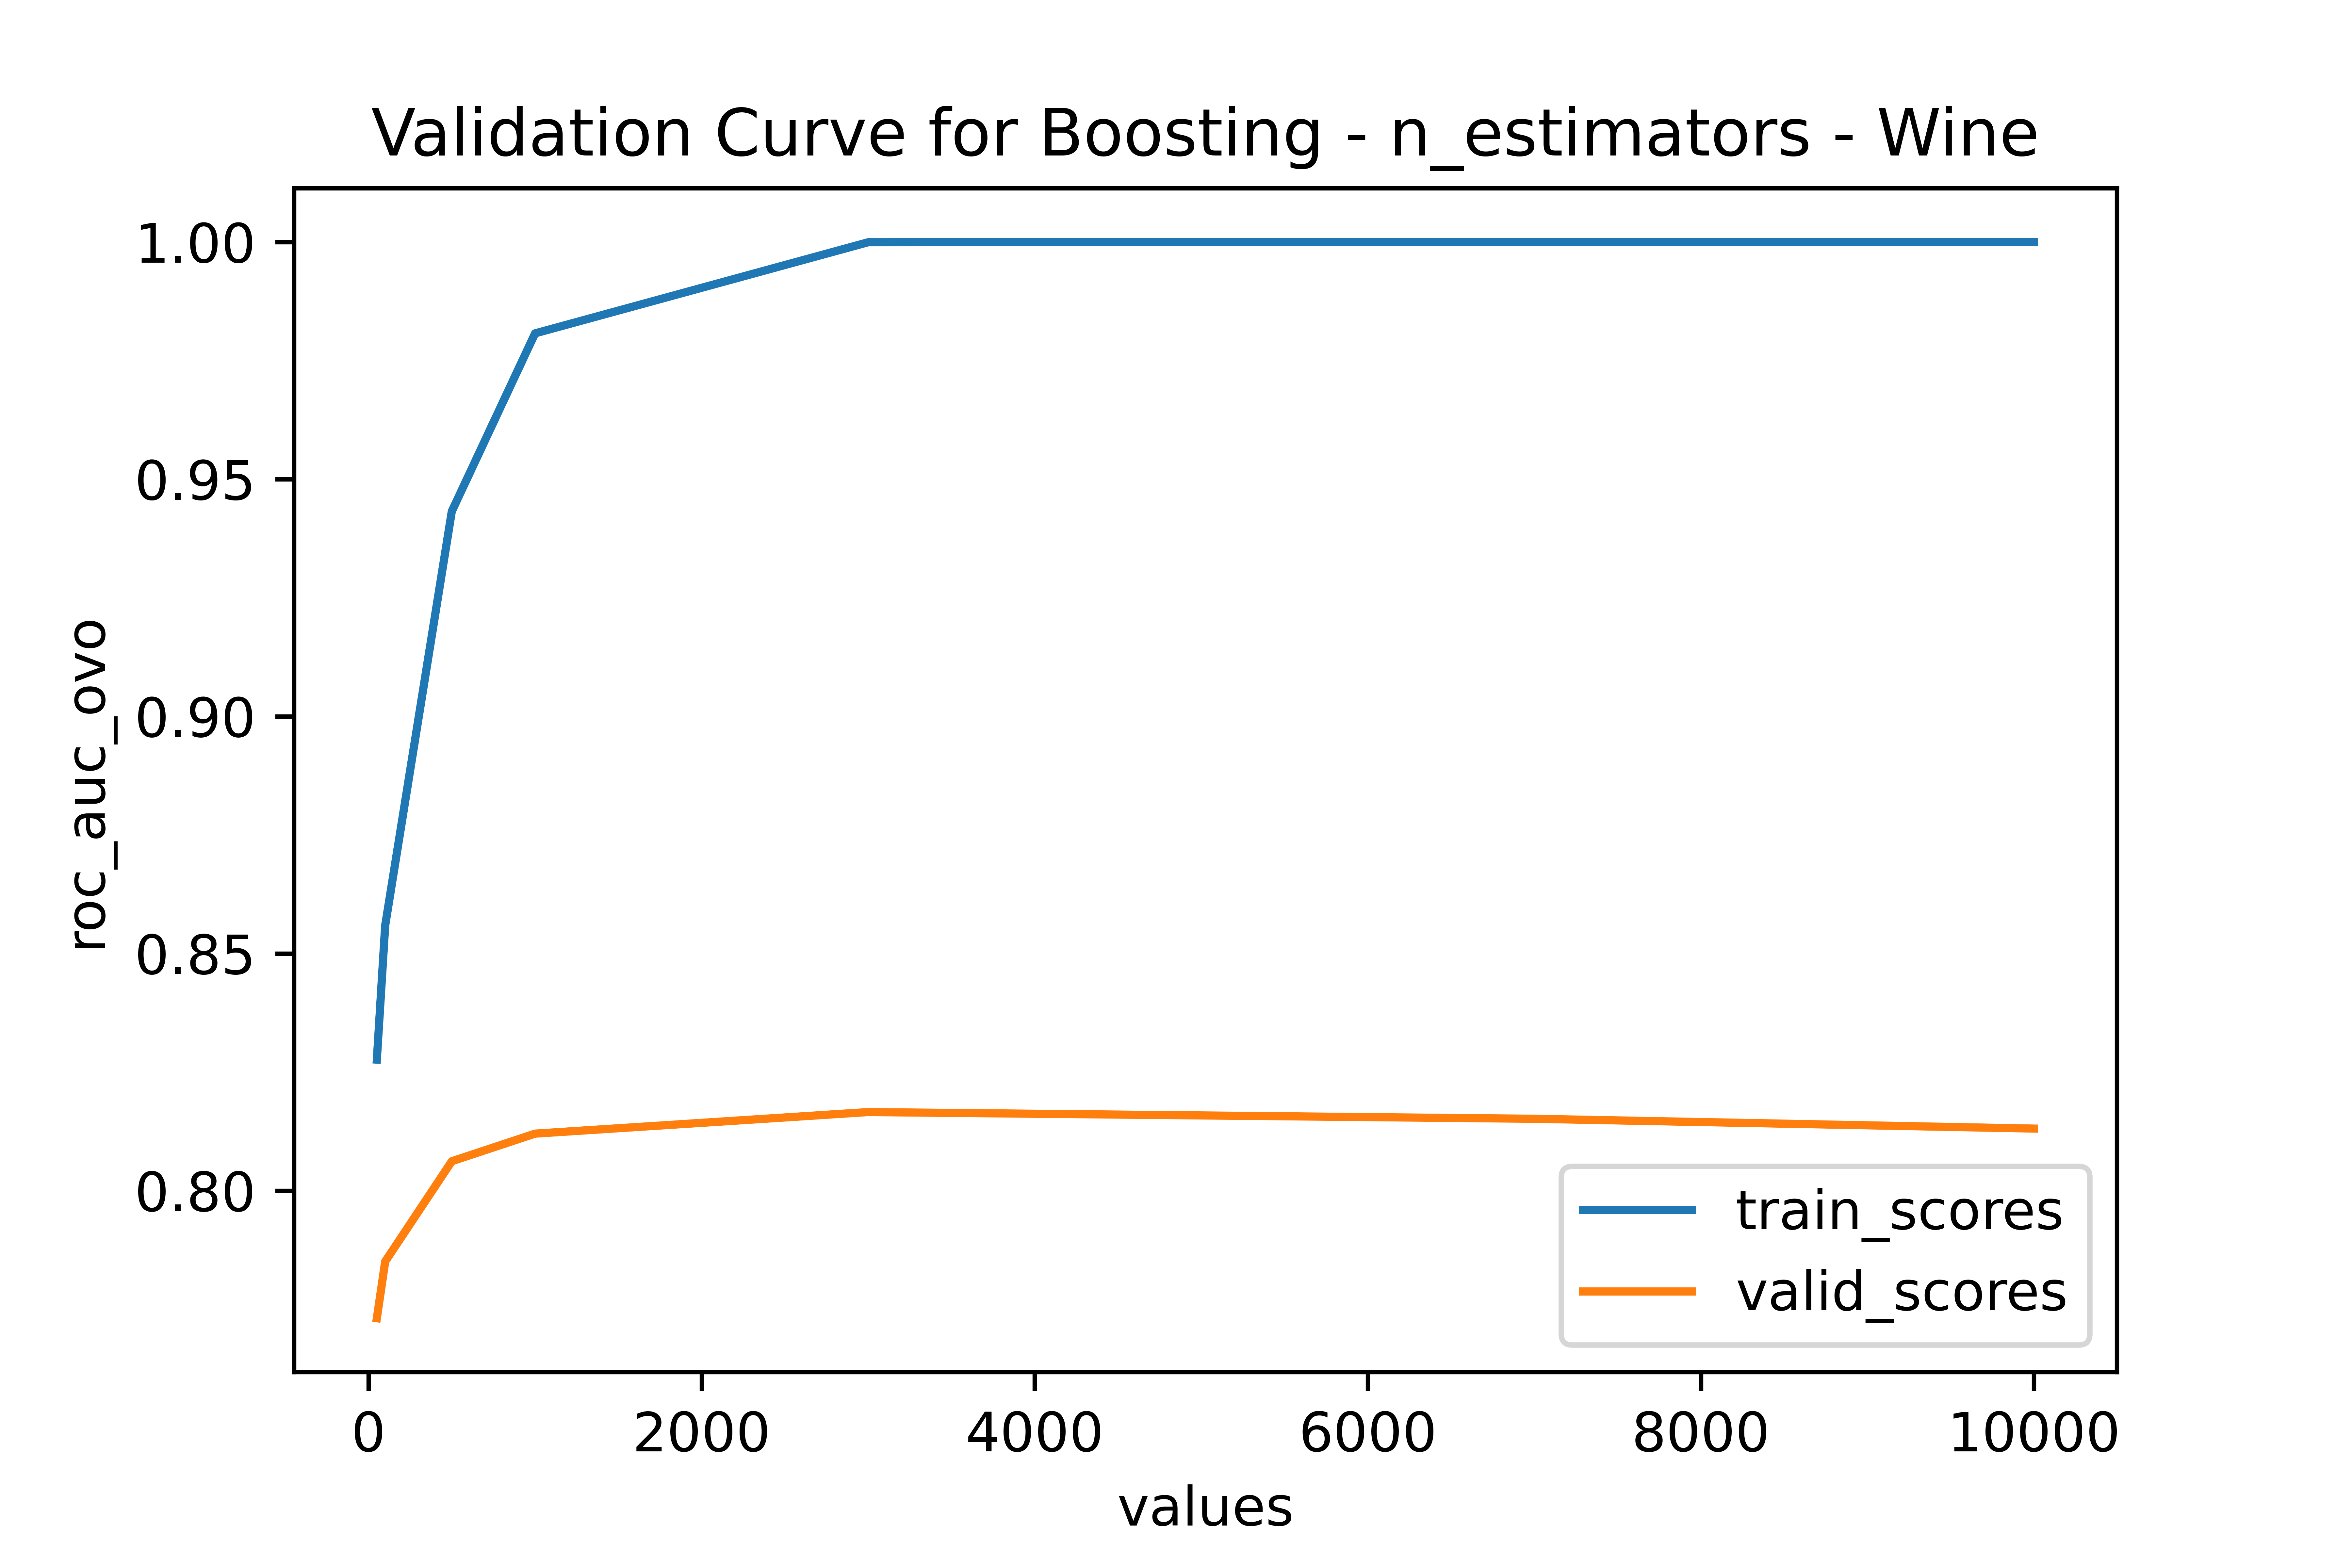
\includegraphics[width=3.4in]{Figures/Wine-0921/GBM/val_curve_0.png}
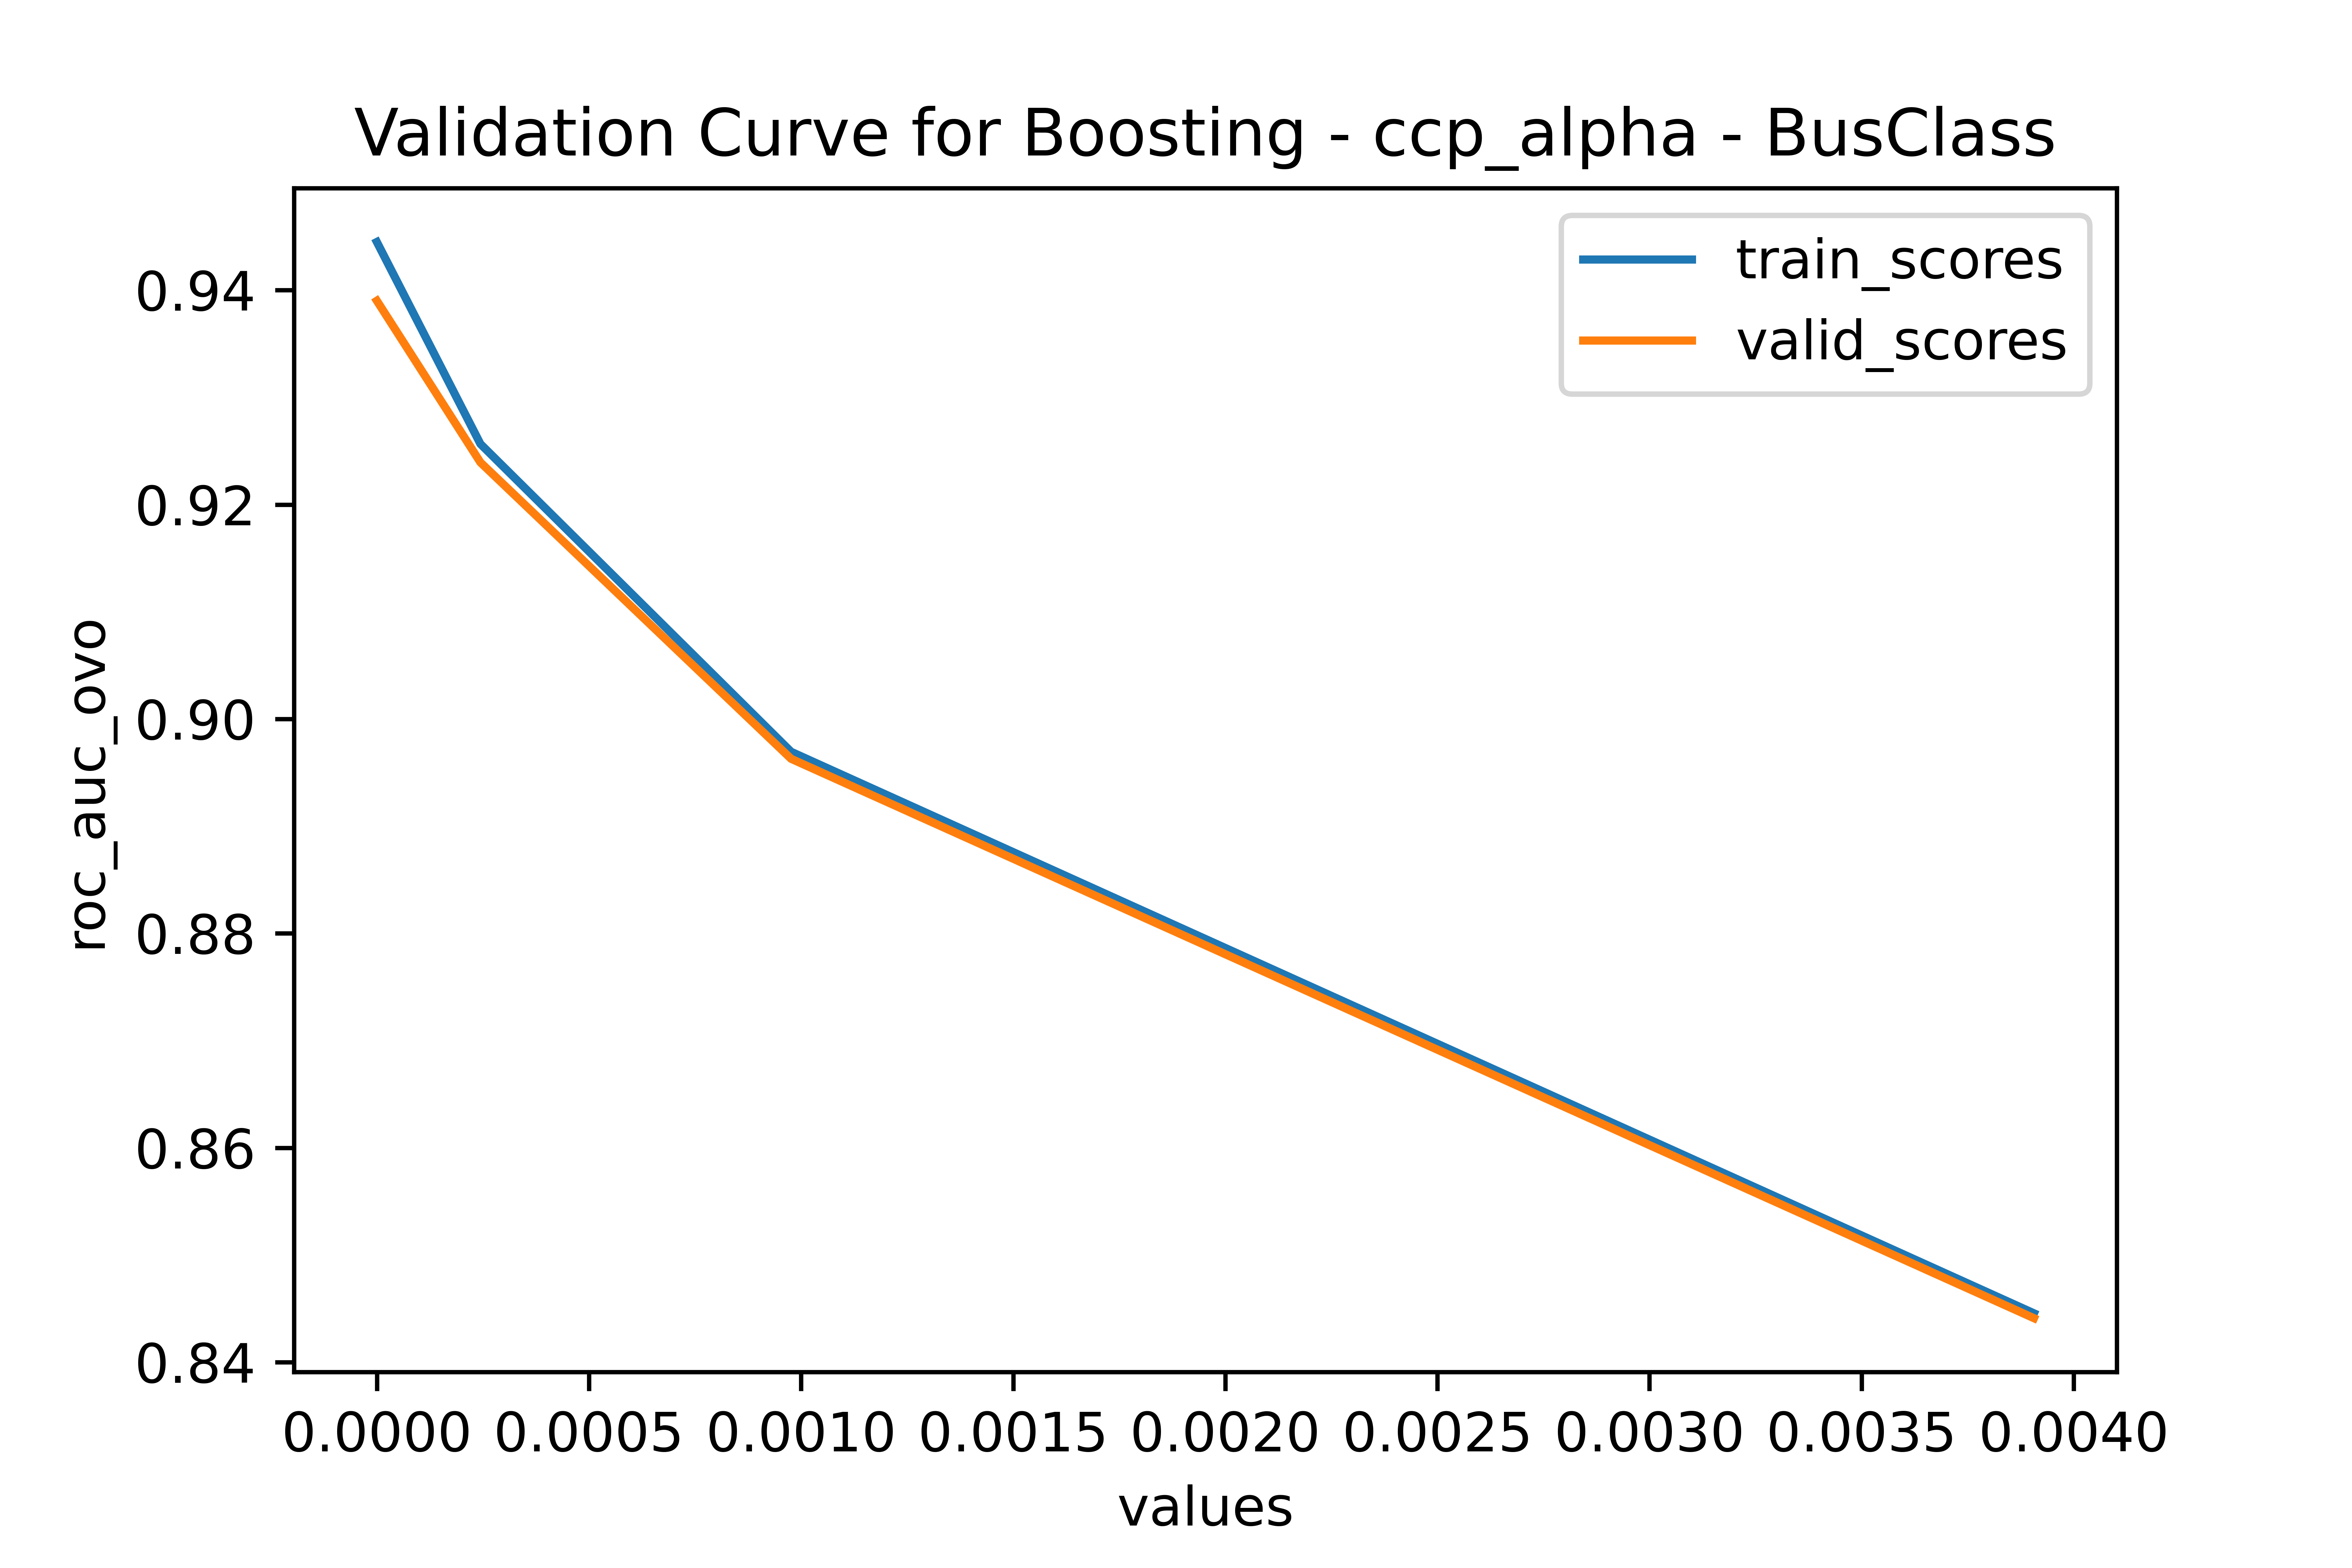
\includegraphics[width=3.4in]{Figures/BusClass-0920/GBM/val_curve_1.png}
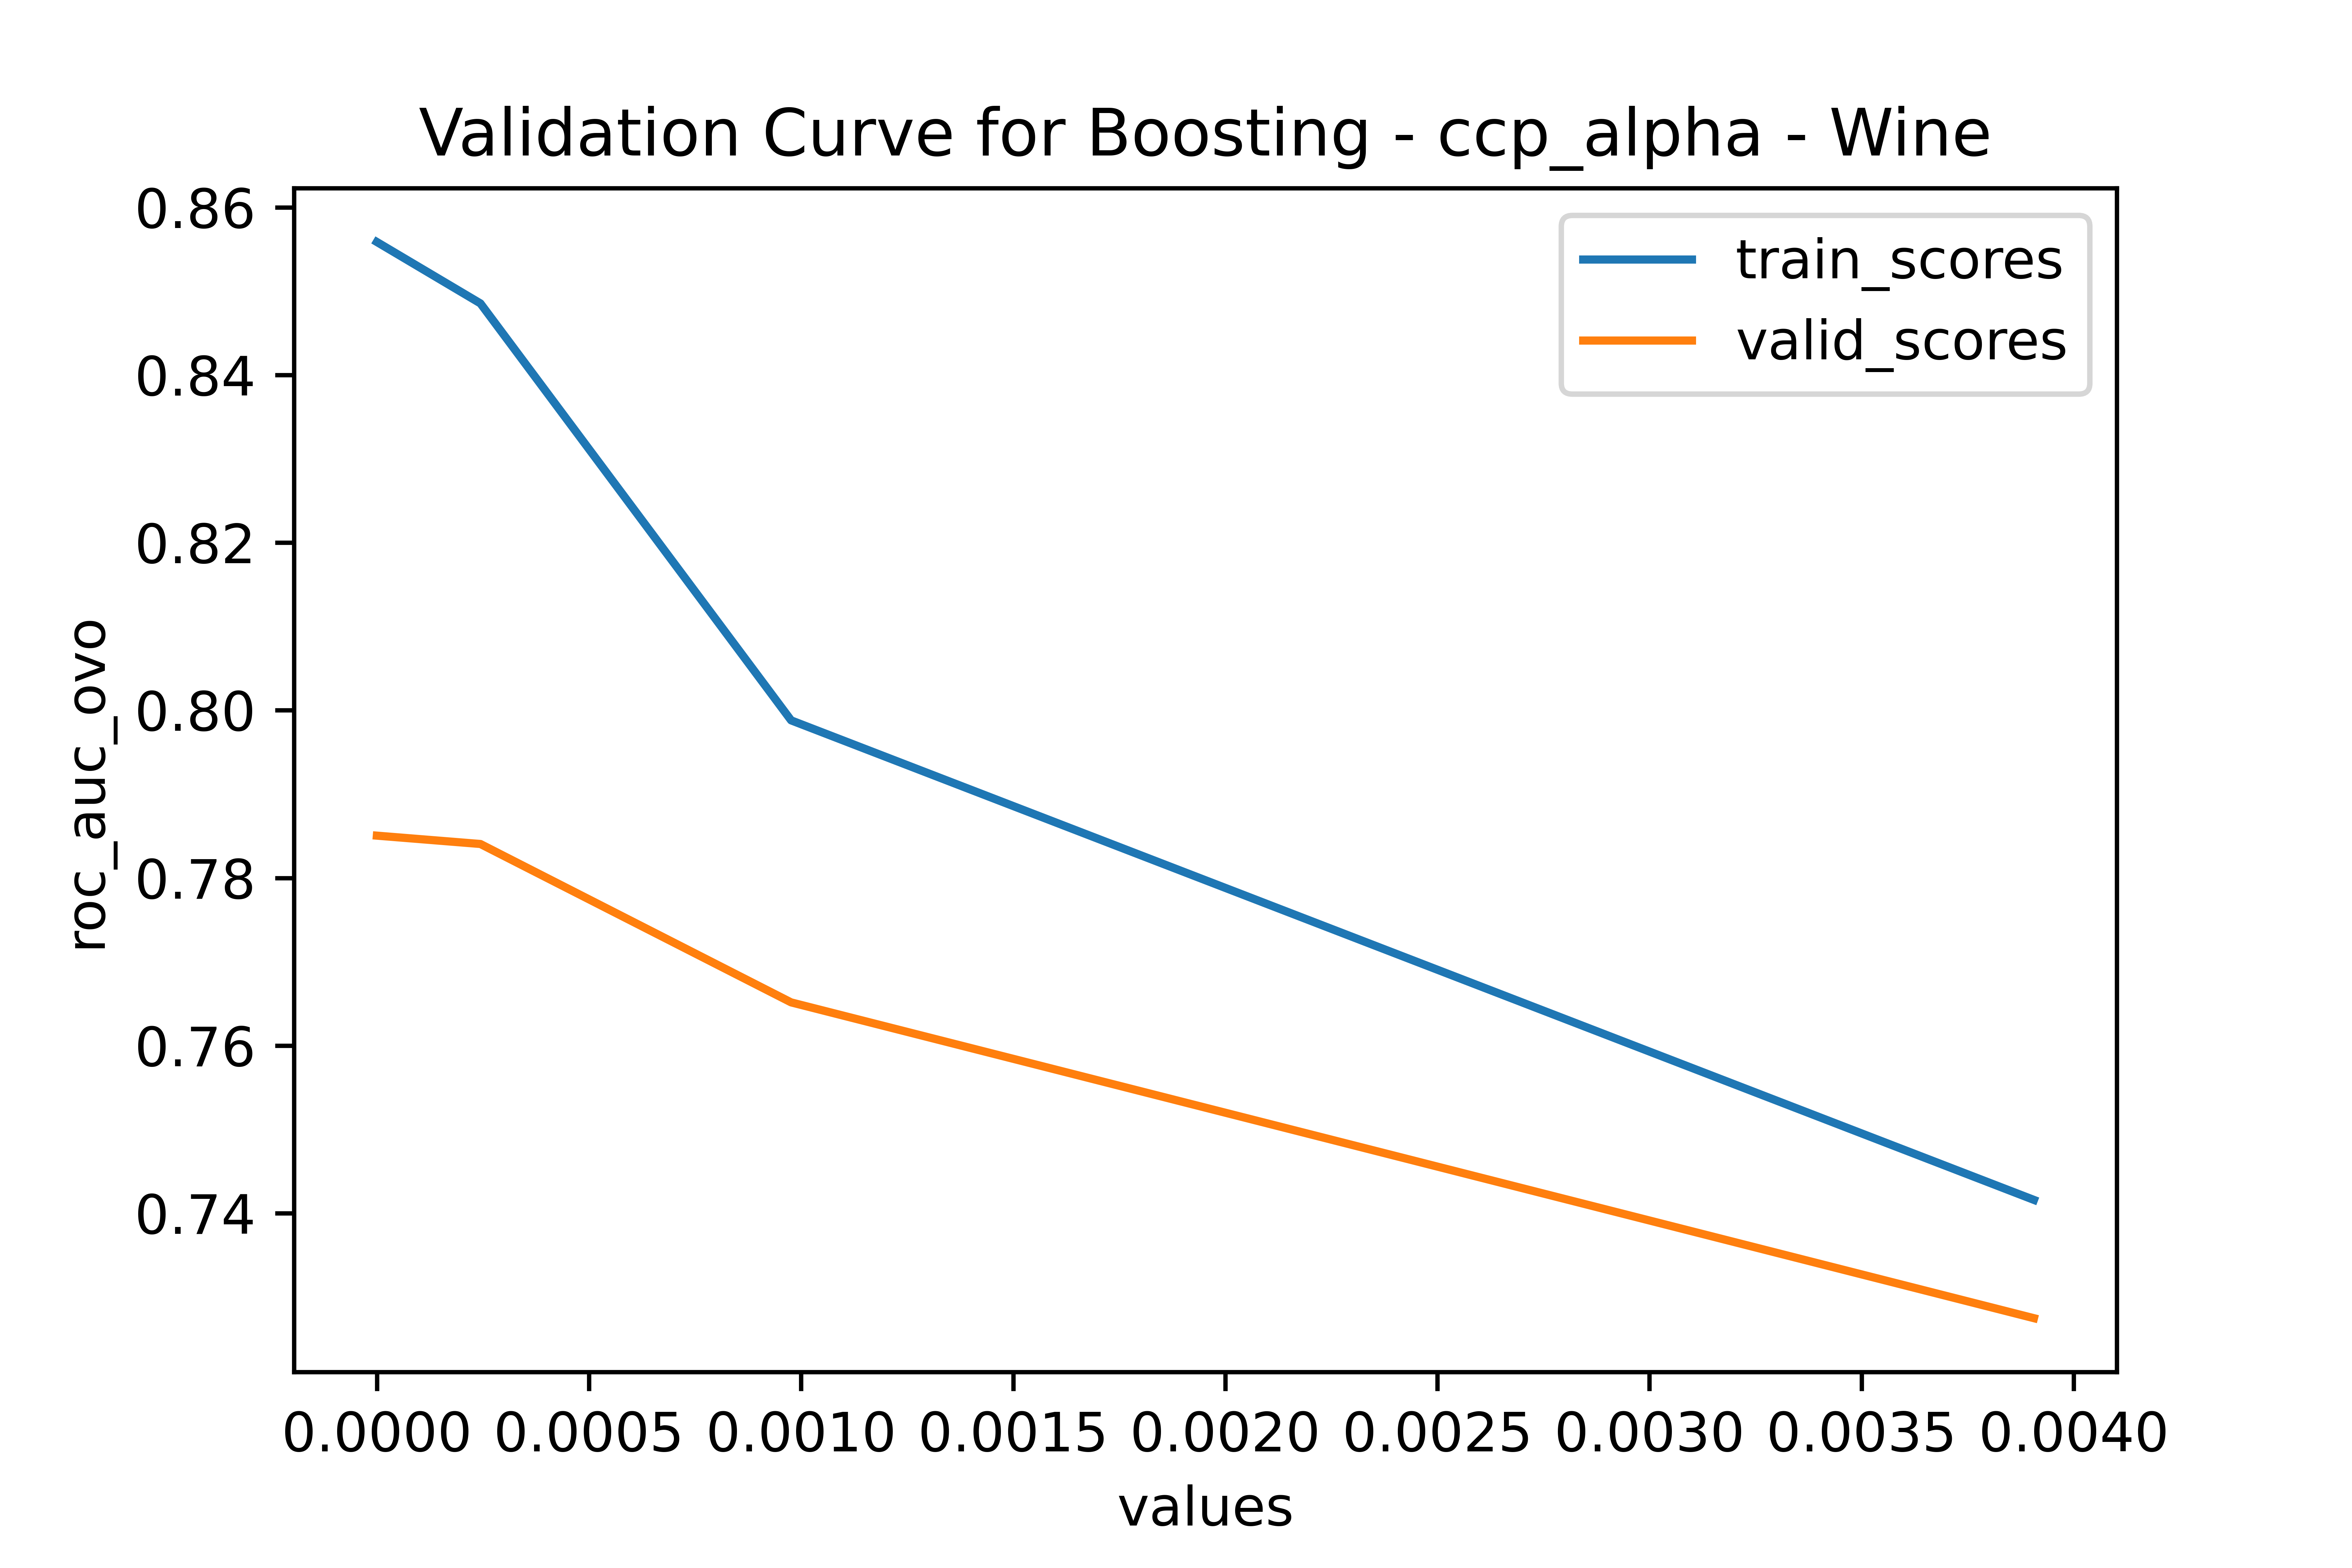
\includegraphics[width=3.4in]{Figures/Wine-0921/GBM/val_curve_1.png}

\subsubsection{Learning Curves}
The wine dataset could have benefited from more data, though the business classification dataset's cross-validation performance was beginning to plateau with the amount of training data we had. I suppose this makes sense given the different number of records in each.

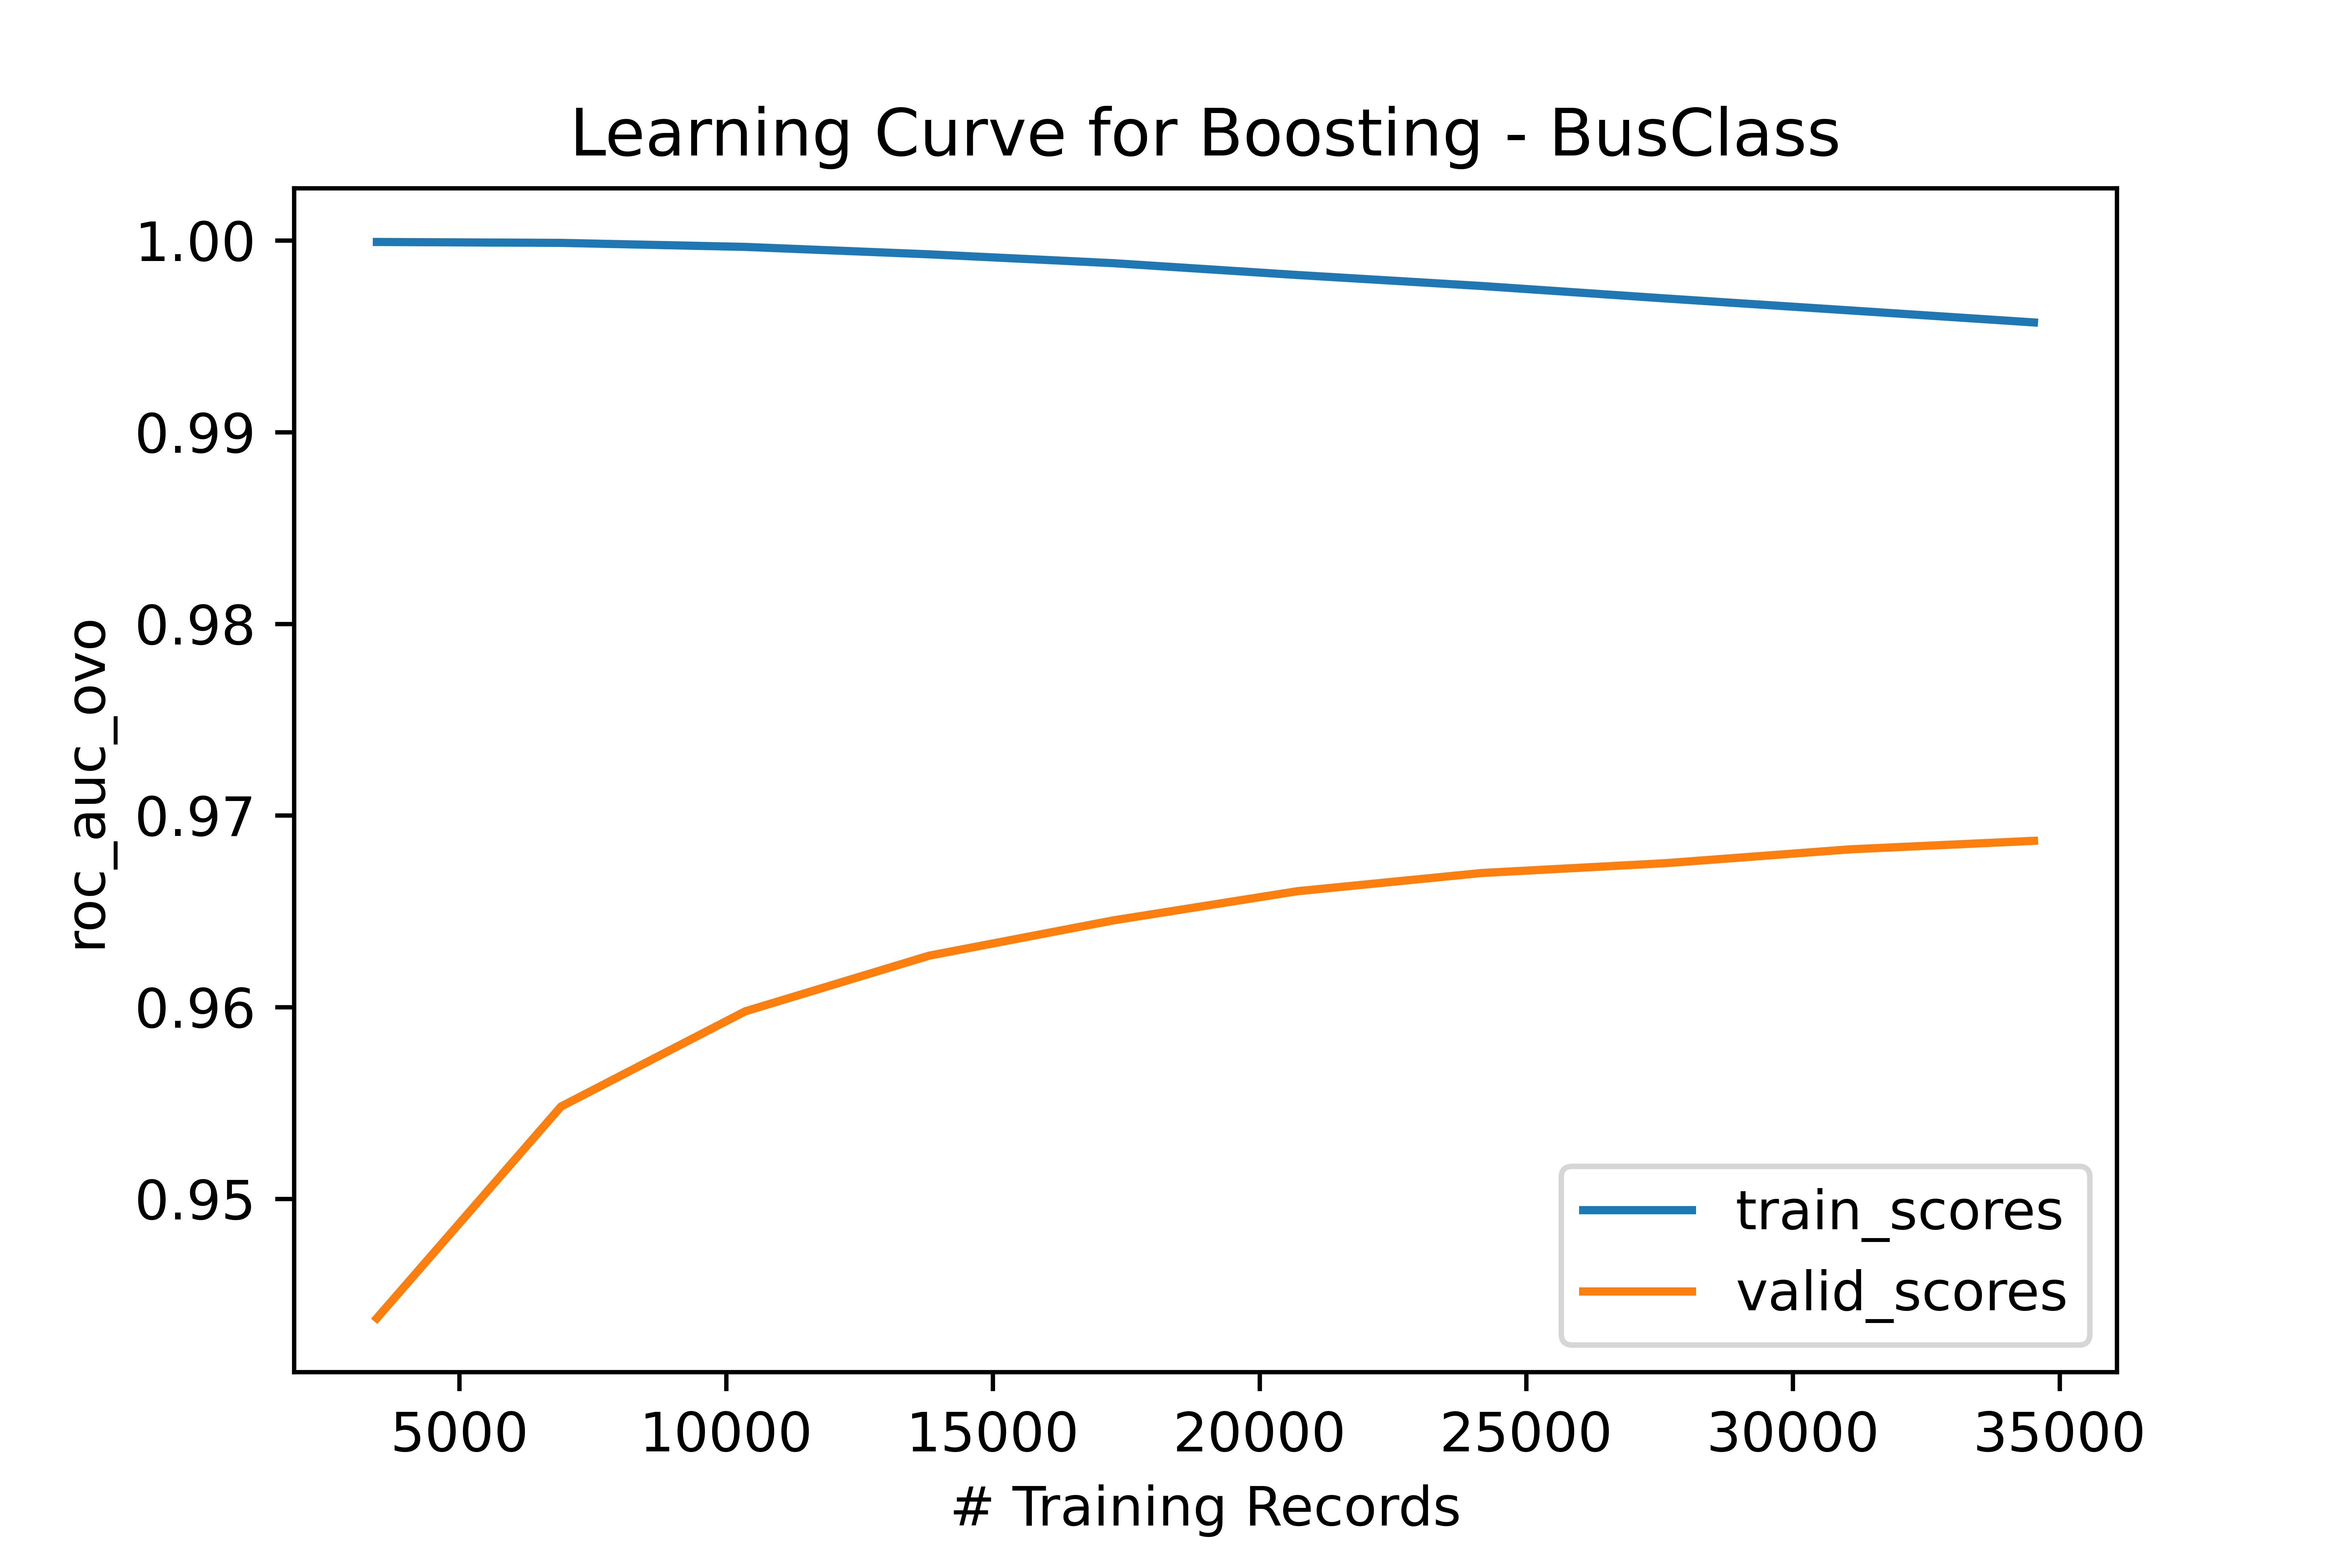
\includegraphics[width=3.4in]{Figures/BusClass-0920/GBM/learn_curve.png}
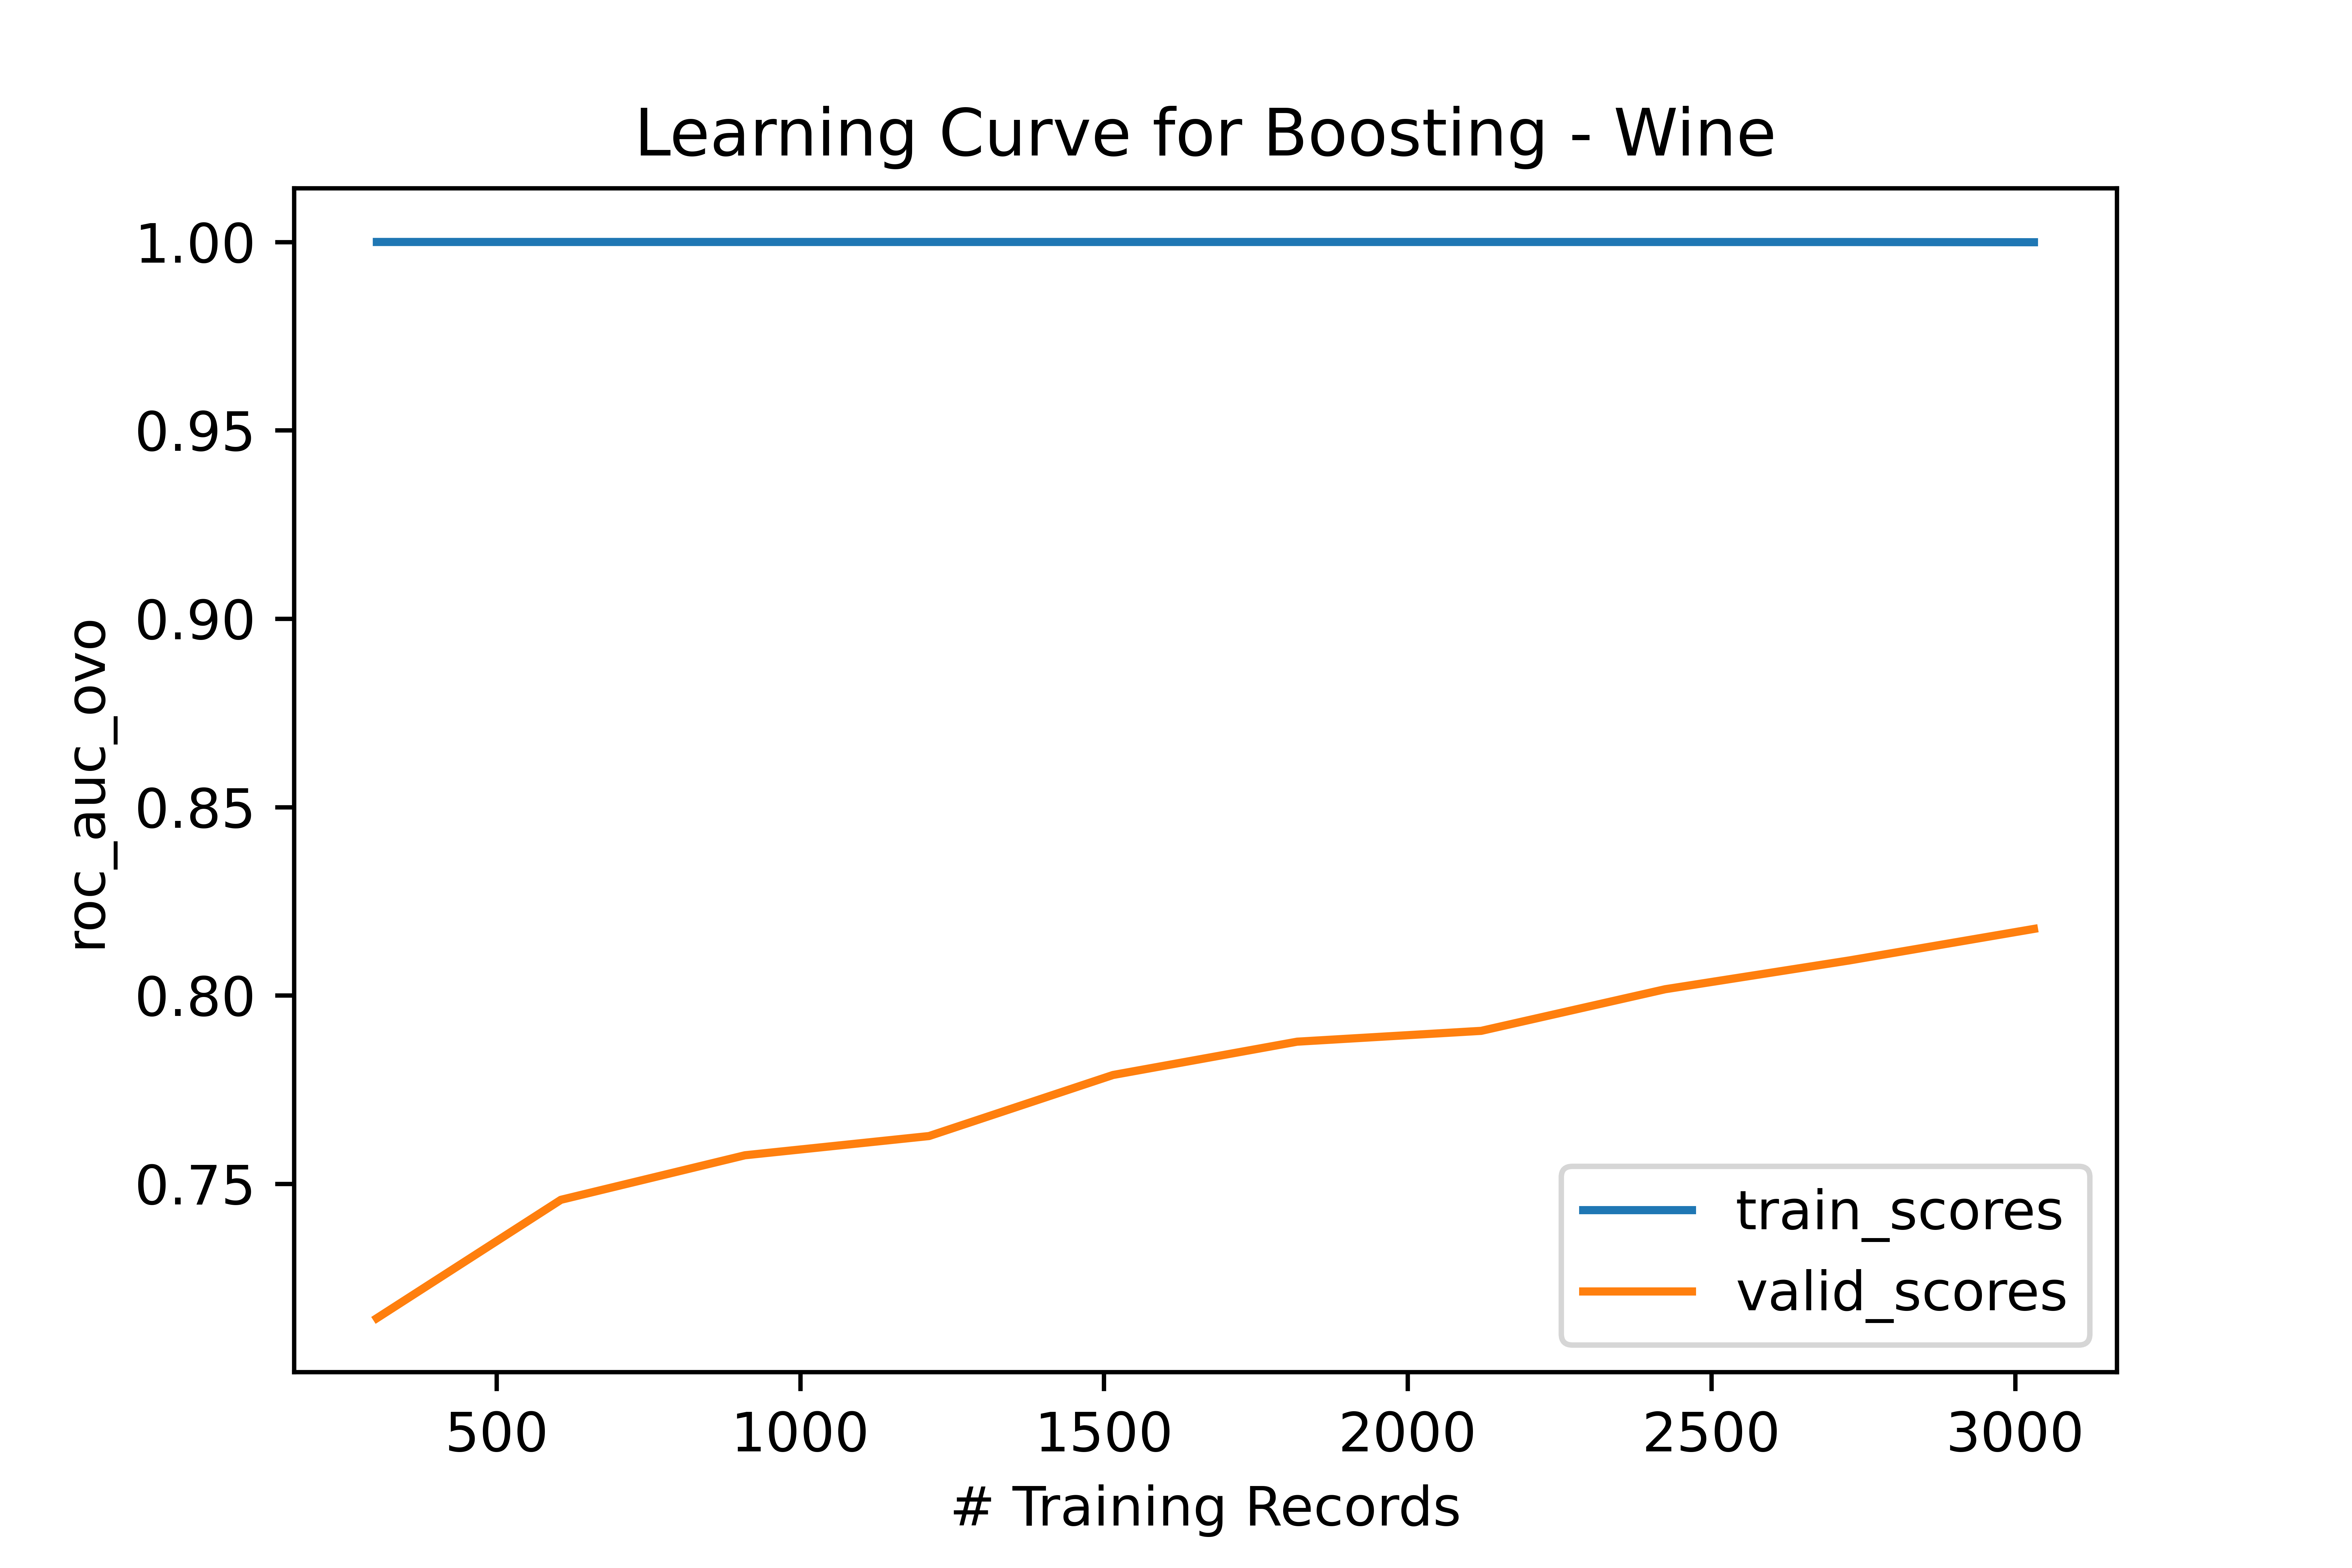
\includegraphics[width=3.4in]{Figures/Wine-0921/GBM/learn_curve.png}

\subsubsection{Wall Clock Time}

Once again, we see a fit time with a linear relationship to the amount of training data. The score time was roughly constant with respect to training data. I reduced the amount of time required for fitting by only considering a relatively small subset of columns for each tree.

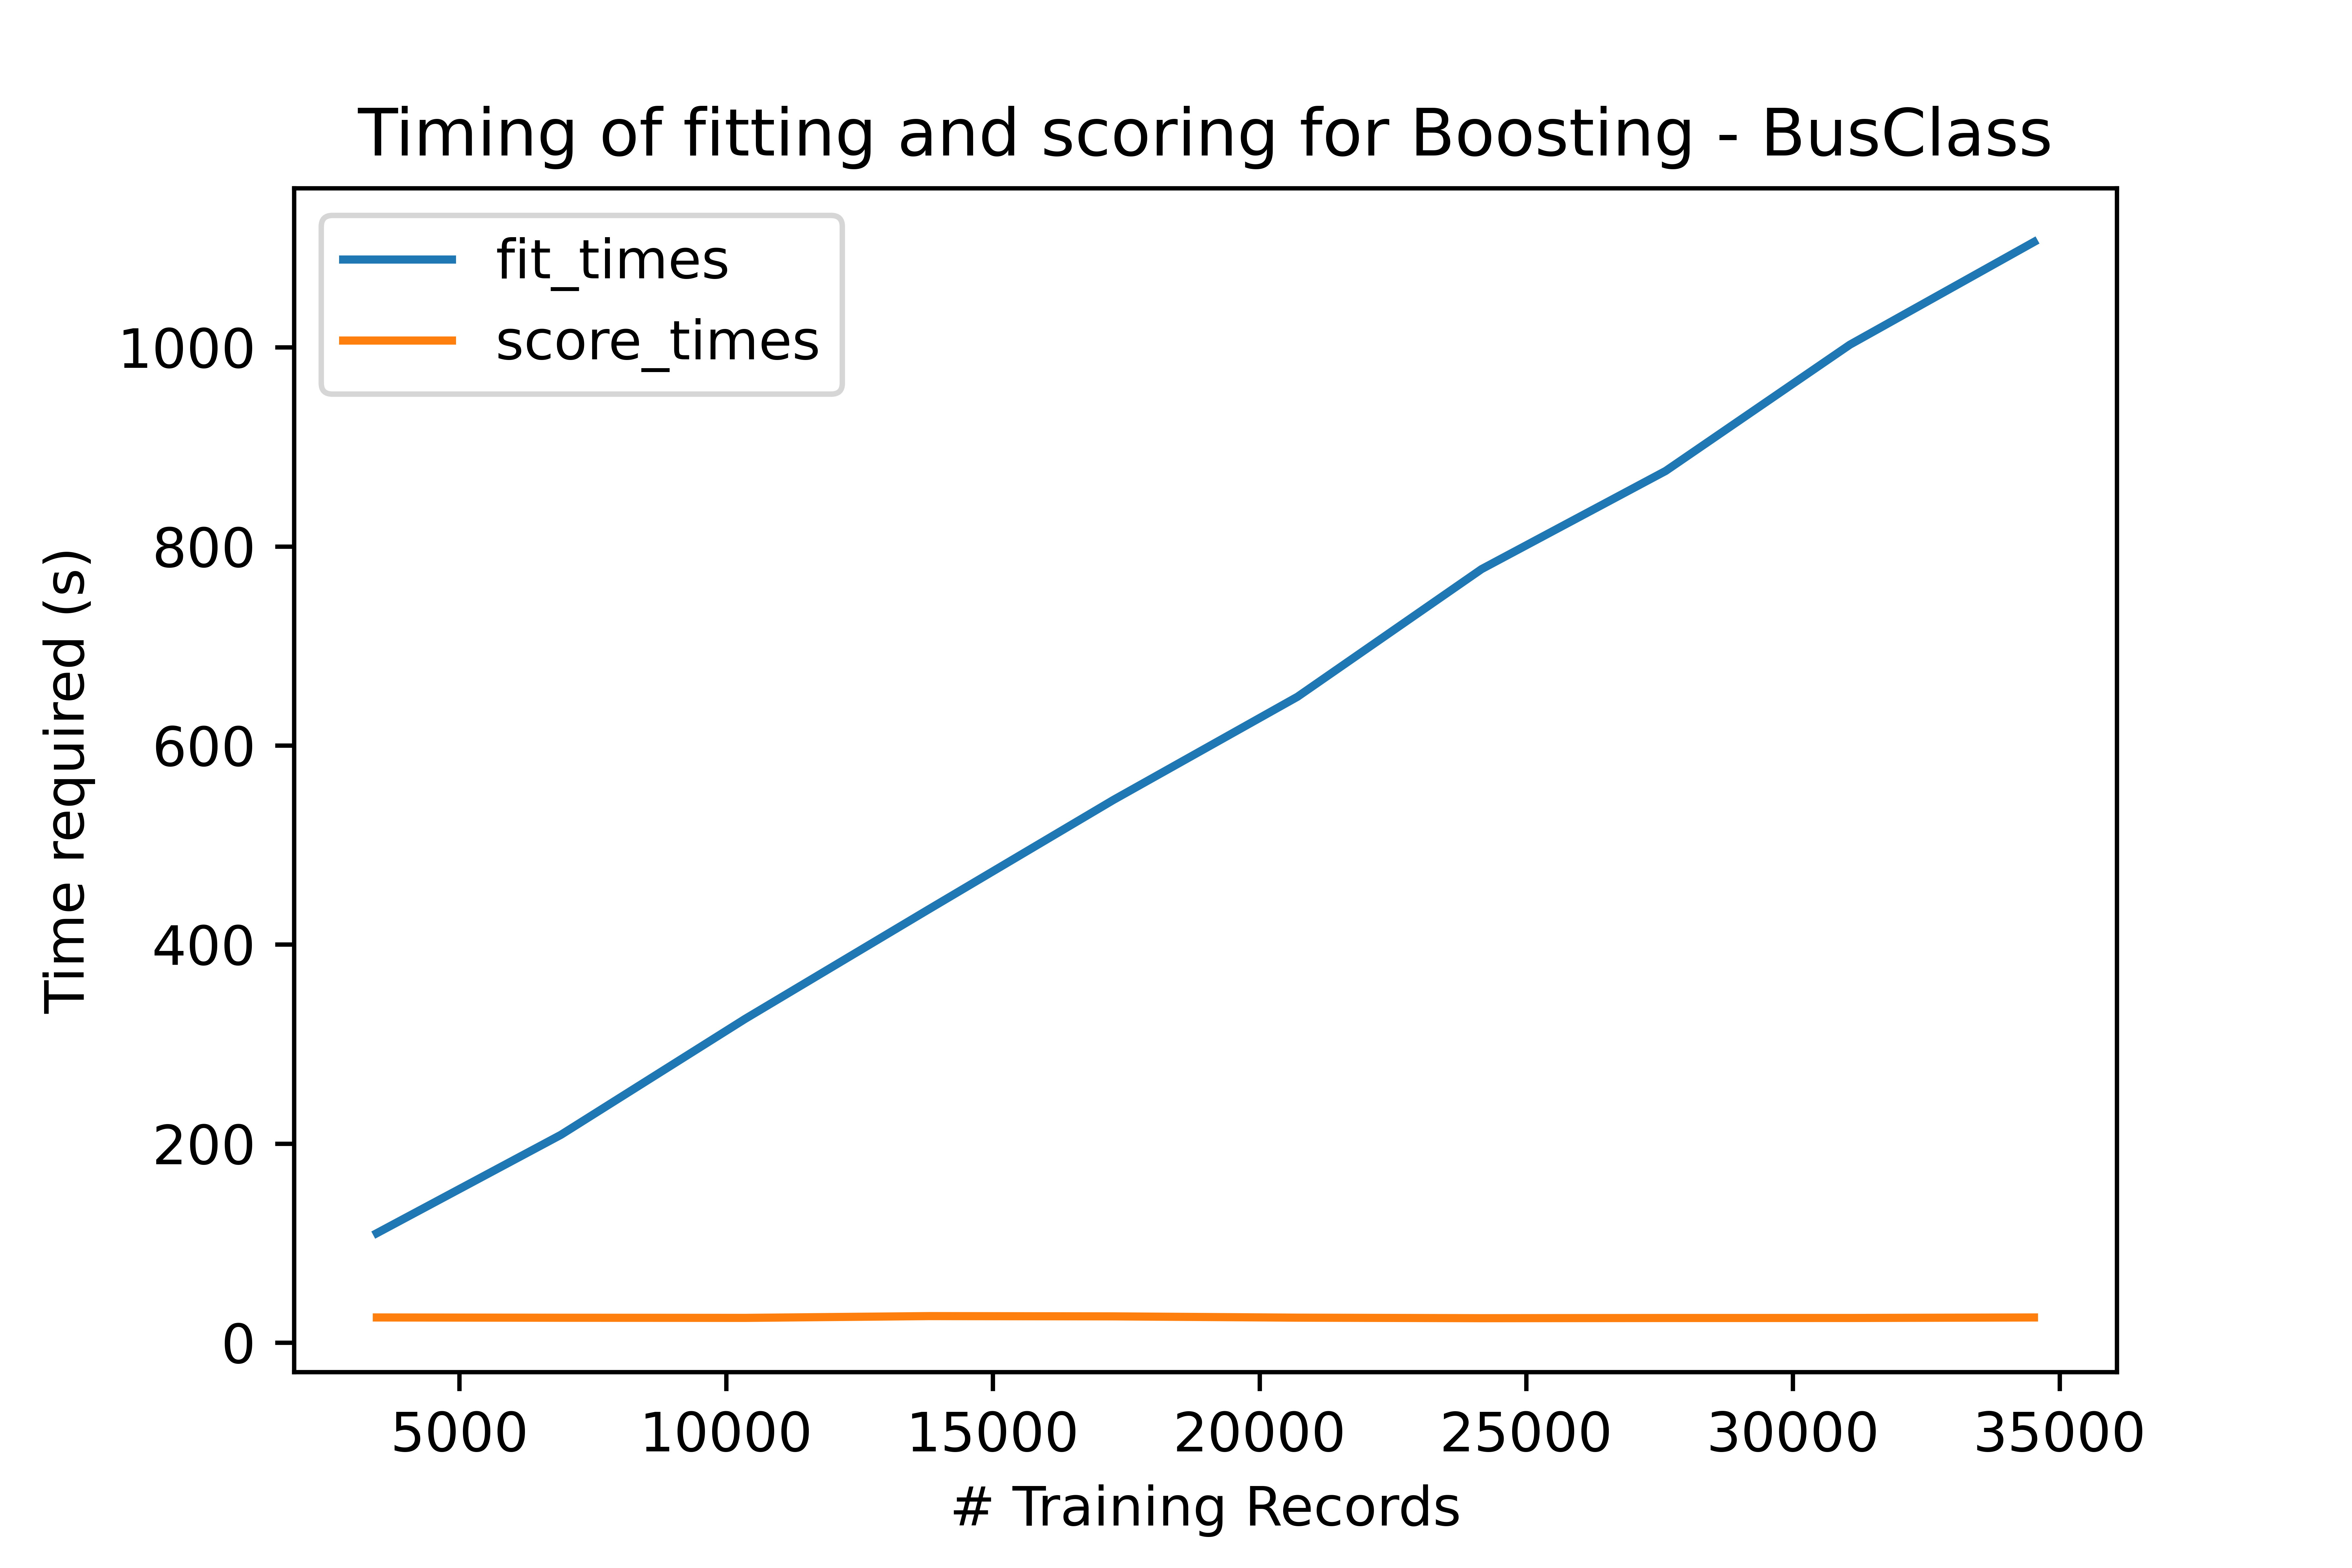
\includegraphics[width=3.4in]{Figures/BusClass-0920/GBM/time_curve.png}
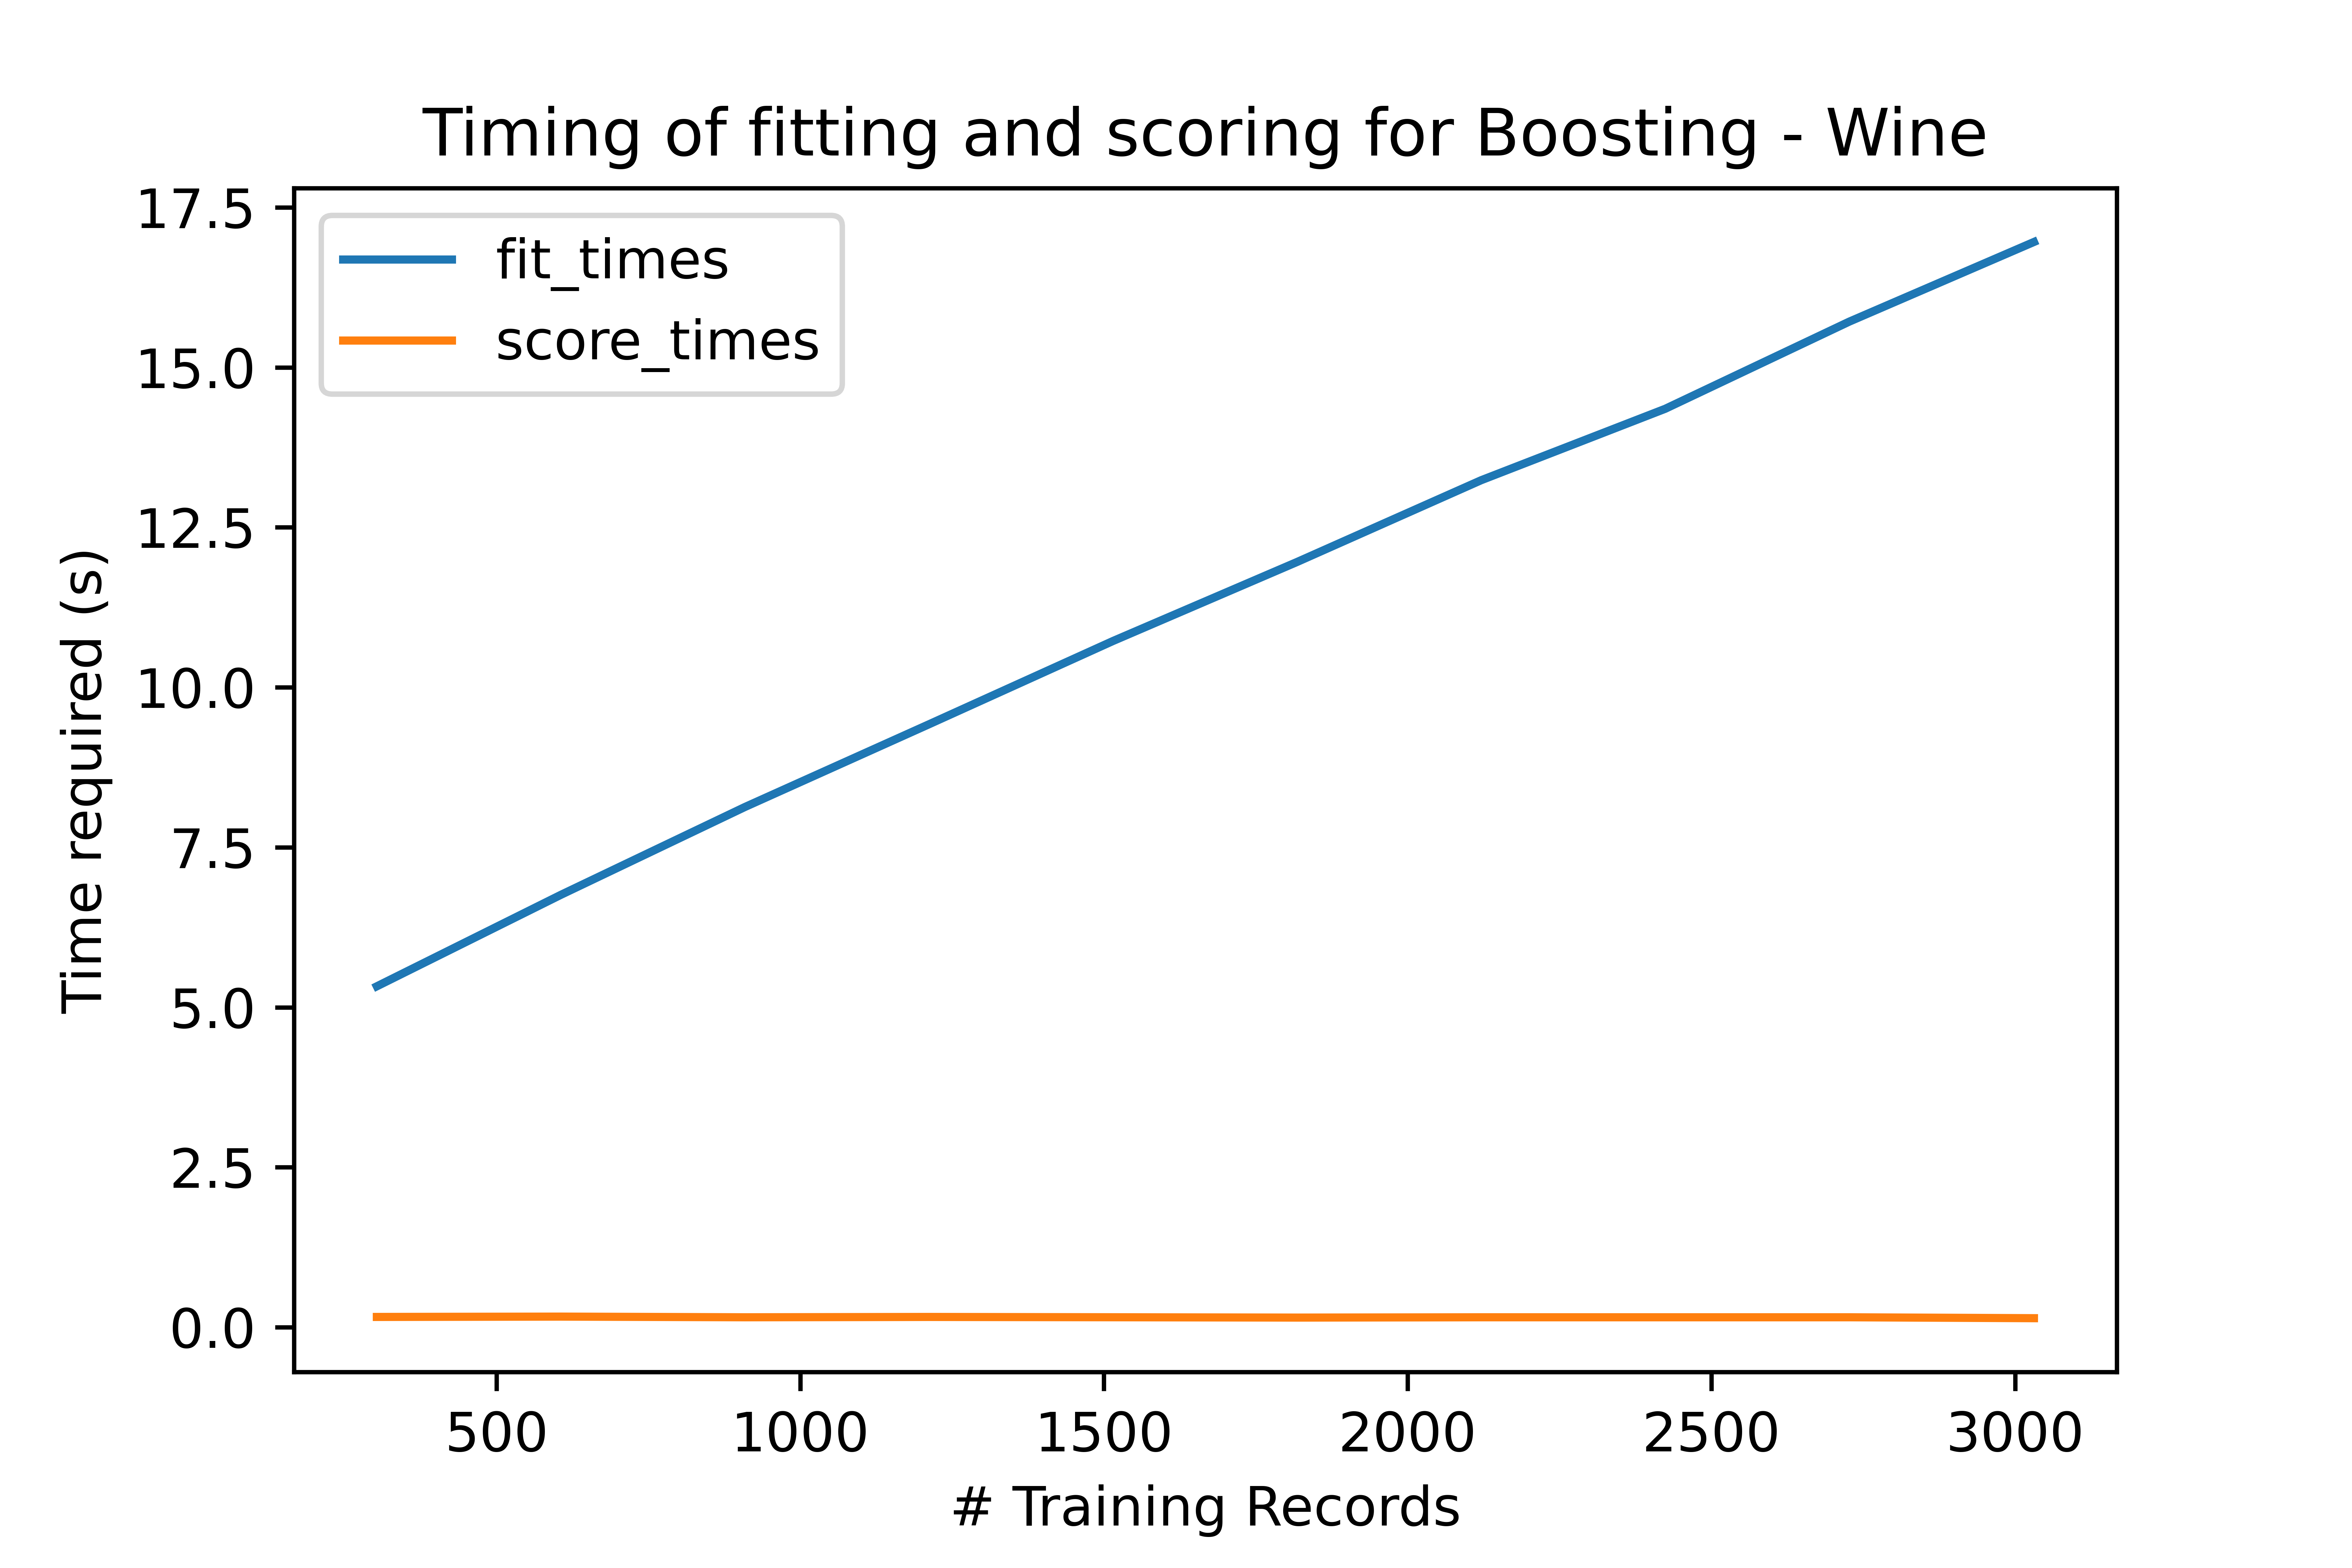
\includegraphics[width=3.4in]{Figures/Wine-0921/GBM/time_curve.png}


\subsection{SVM}

\subsubsection{Hyperparameter Tuning}

Fascinatingly, the correct kernel choice varies considerably across our two datasets. For the business classification dataset, a linear kernel performed much better than a polynomial or RBF kernel. However for our wine dataset, none performed particularly well (the polynomial kernel was worse than random chance), but the RBF kernel performed the best.

In terms of regularization, less was better. The C hyperparameter is inversely proportional to the amount of regularization, and we see that as it increases, so does our performance on the business classification side. Though do note that the difference in scores is fairly small. For the wine dataset, we see difficulty capturing signal. I think it is fair to say that these SVMs do not fare well in a multi-classification context.

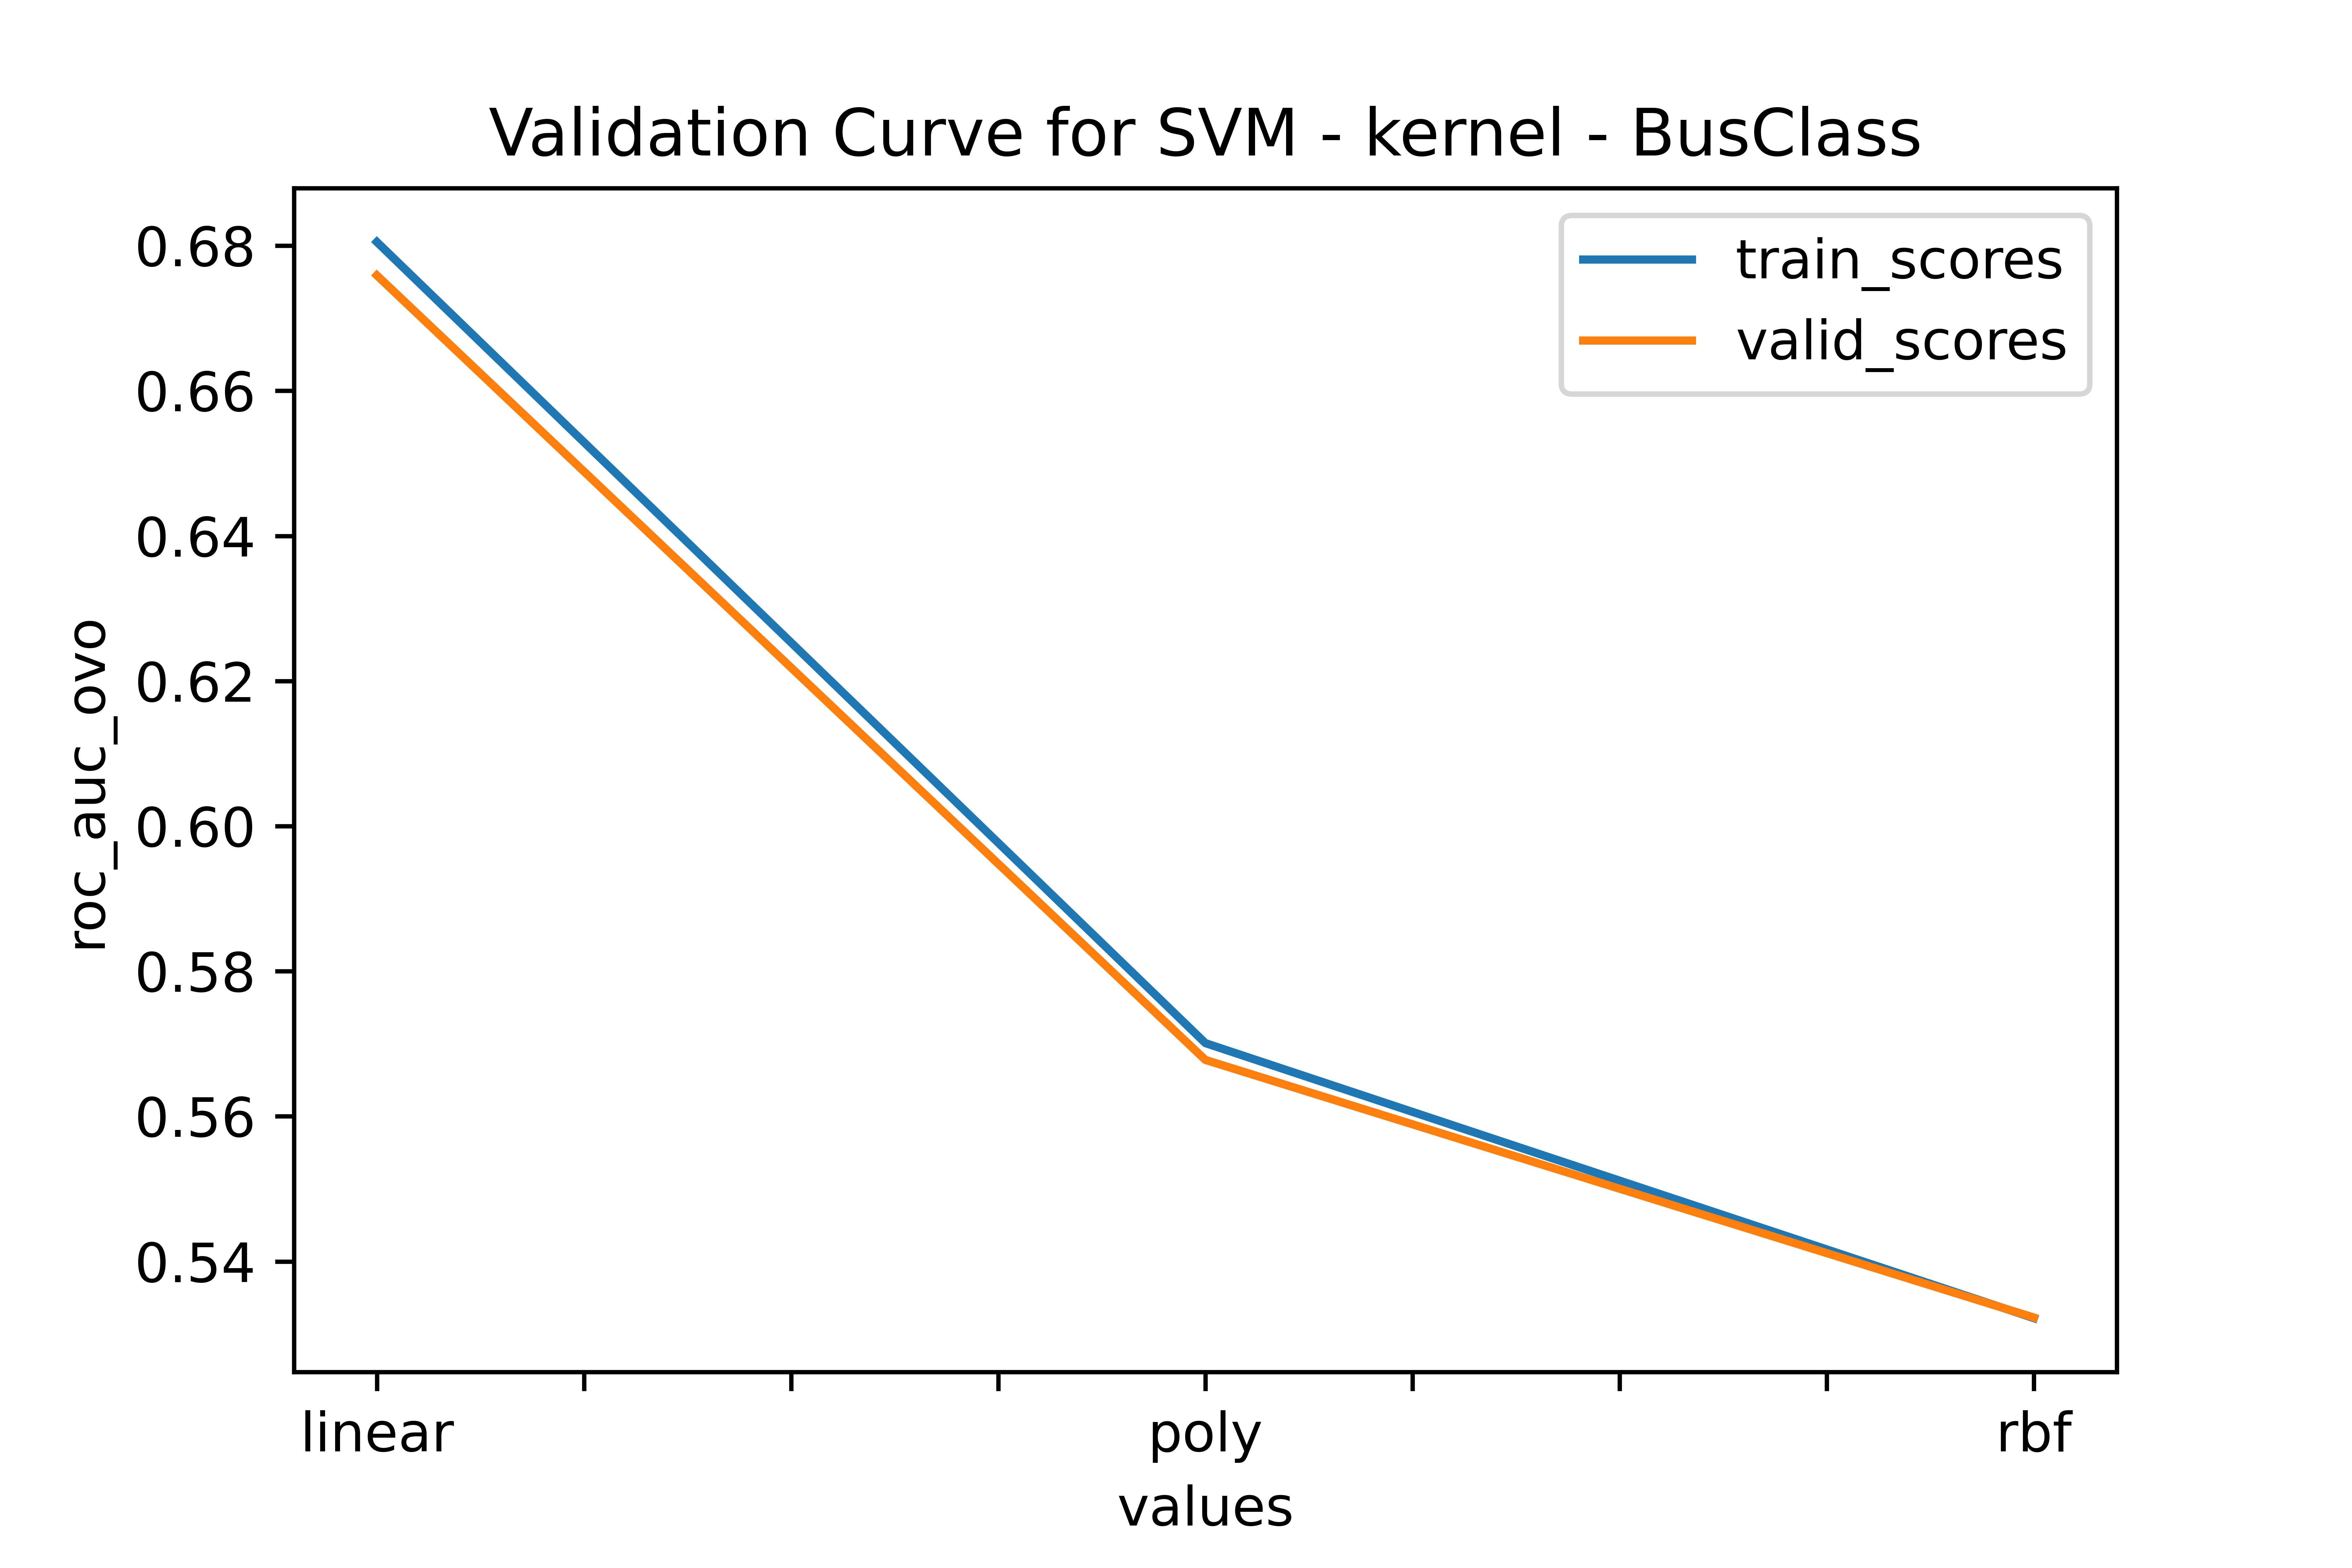
\includegraphics[width=3.4in]{Figures/BusClass-0920/SVM/val_curve_0.png}
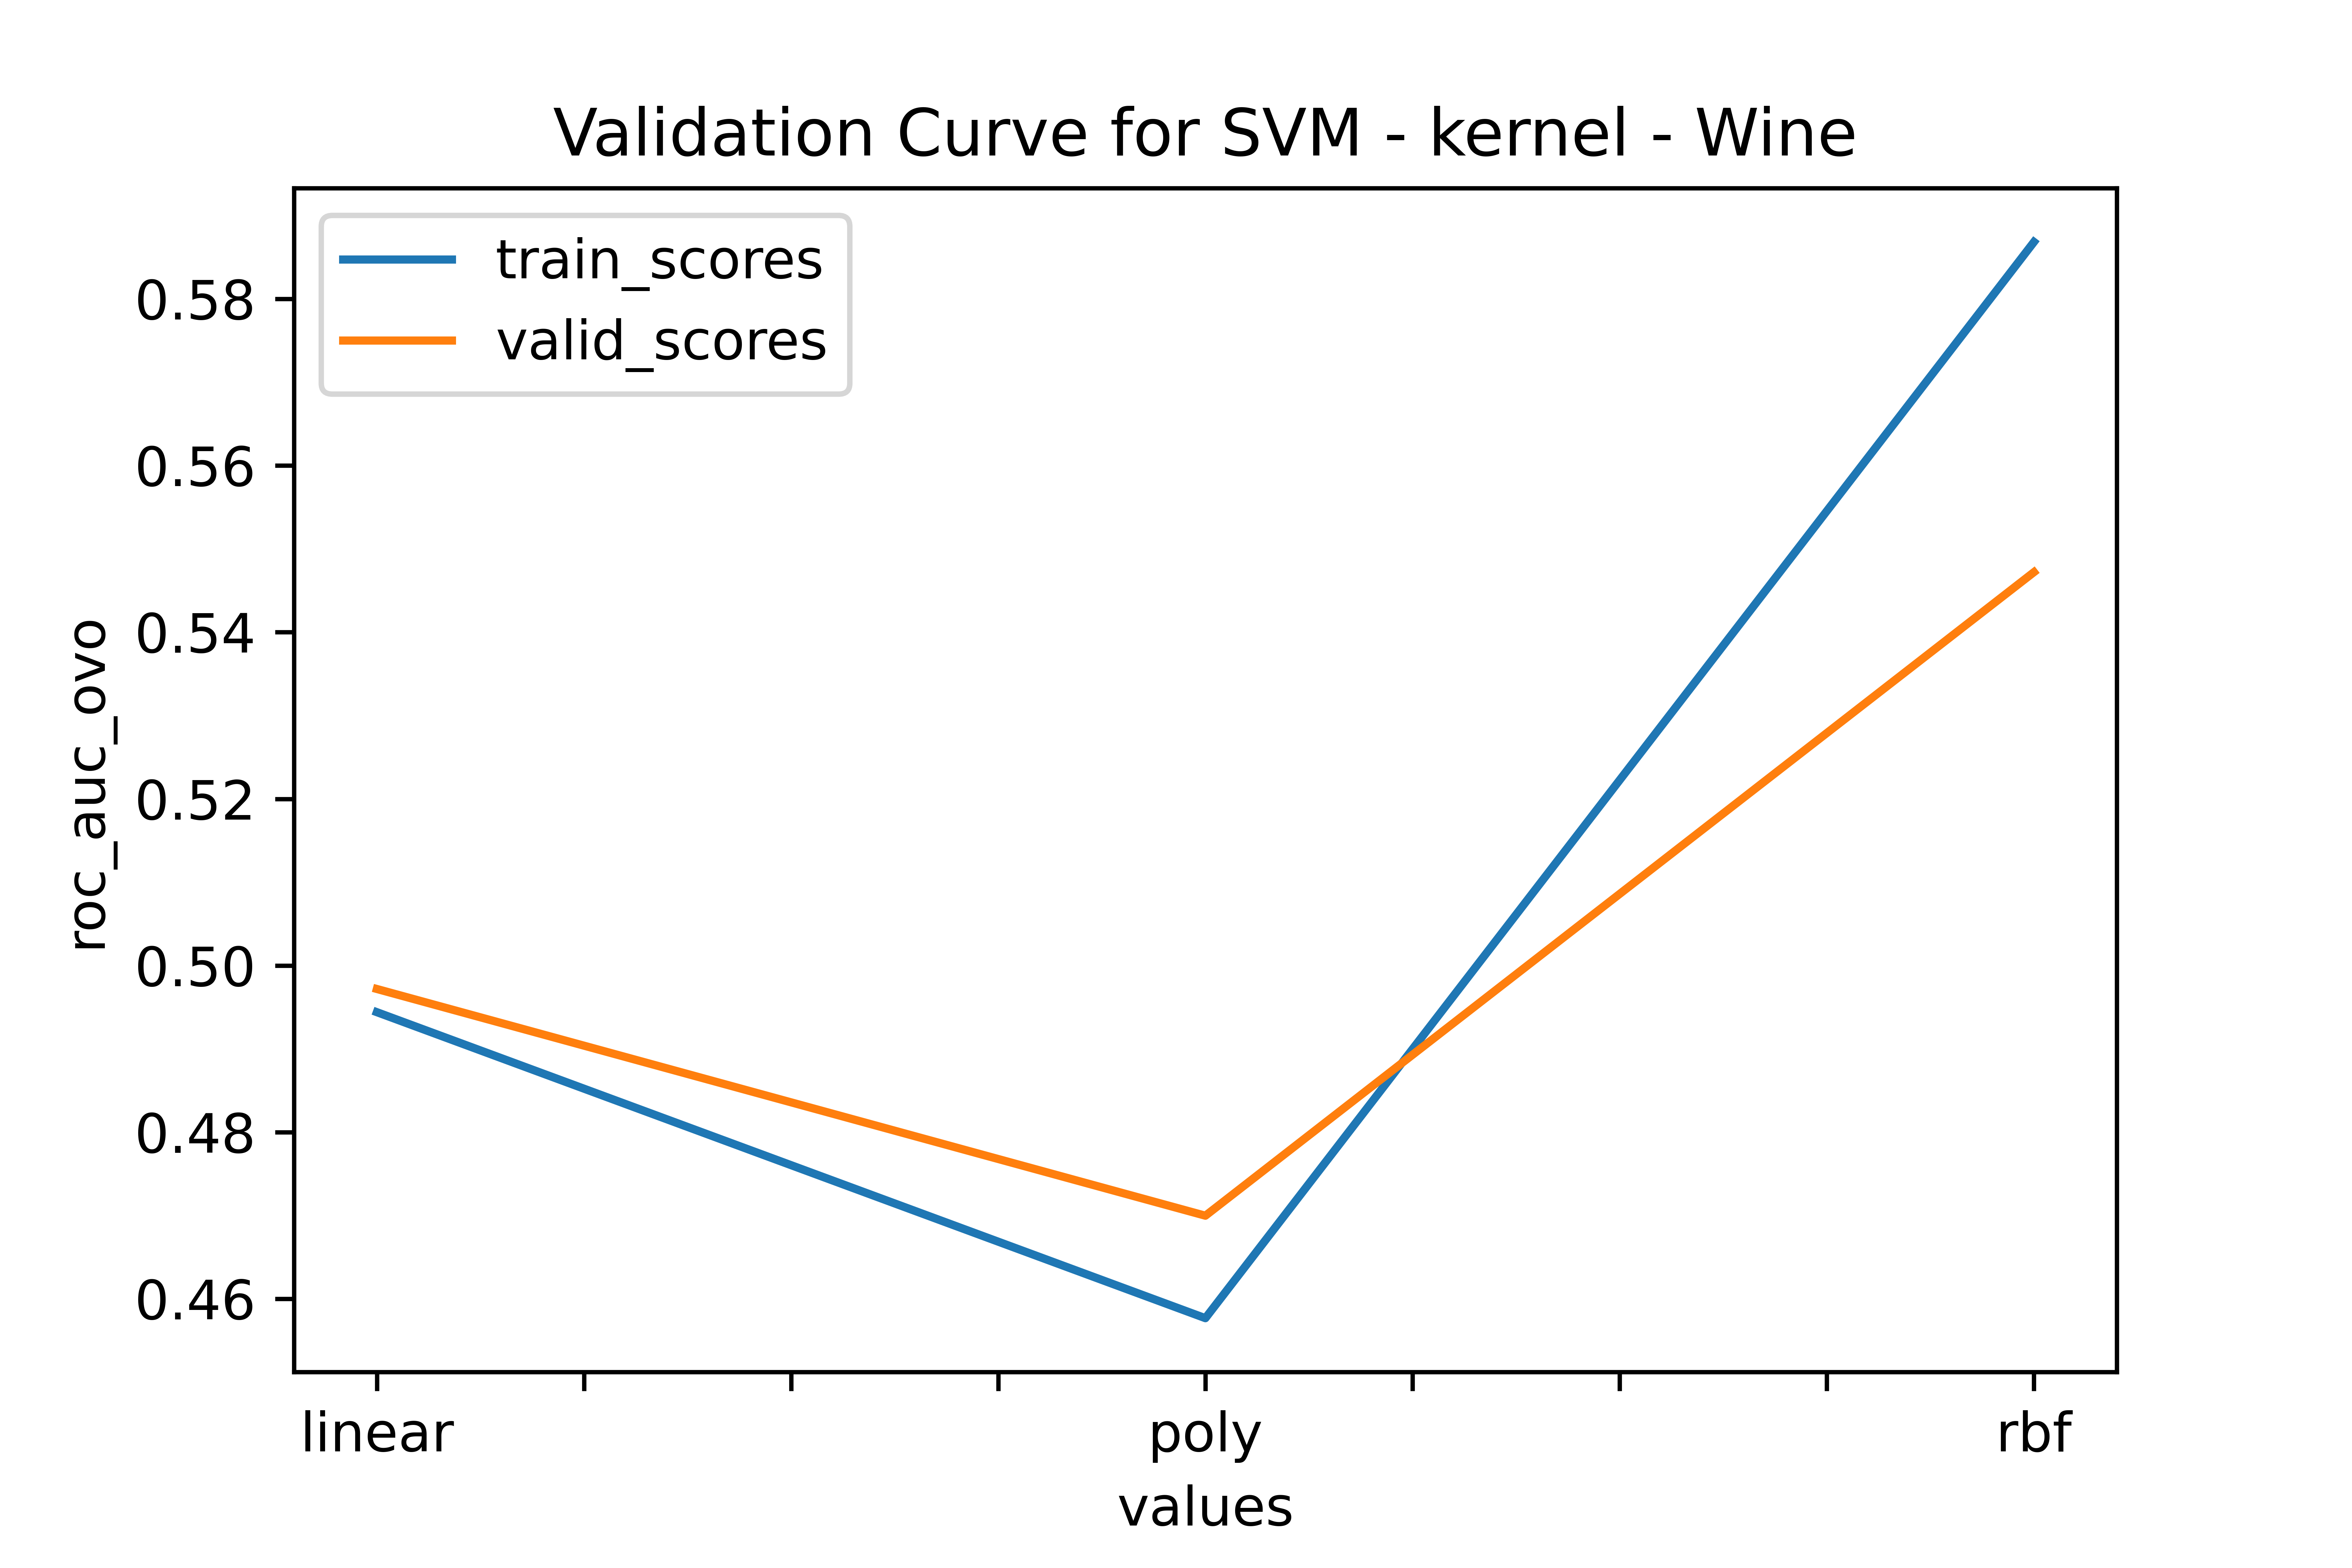
\includegraphics[width=3.4in]{Figures/Wine-0921/SVM/val_curve_0.png}
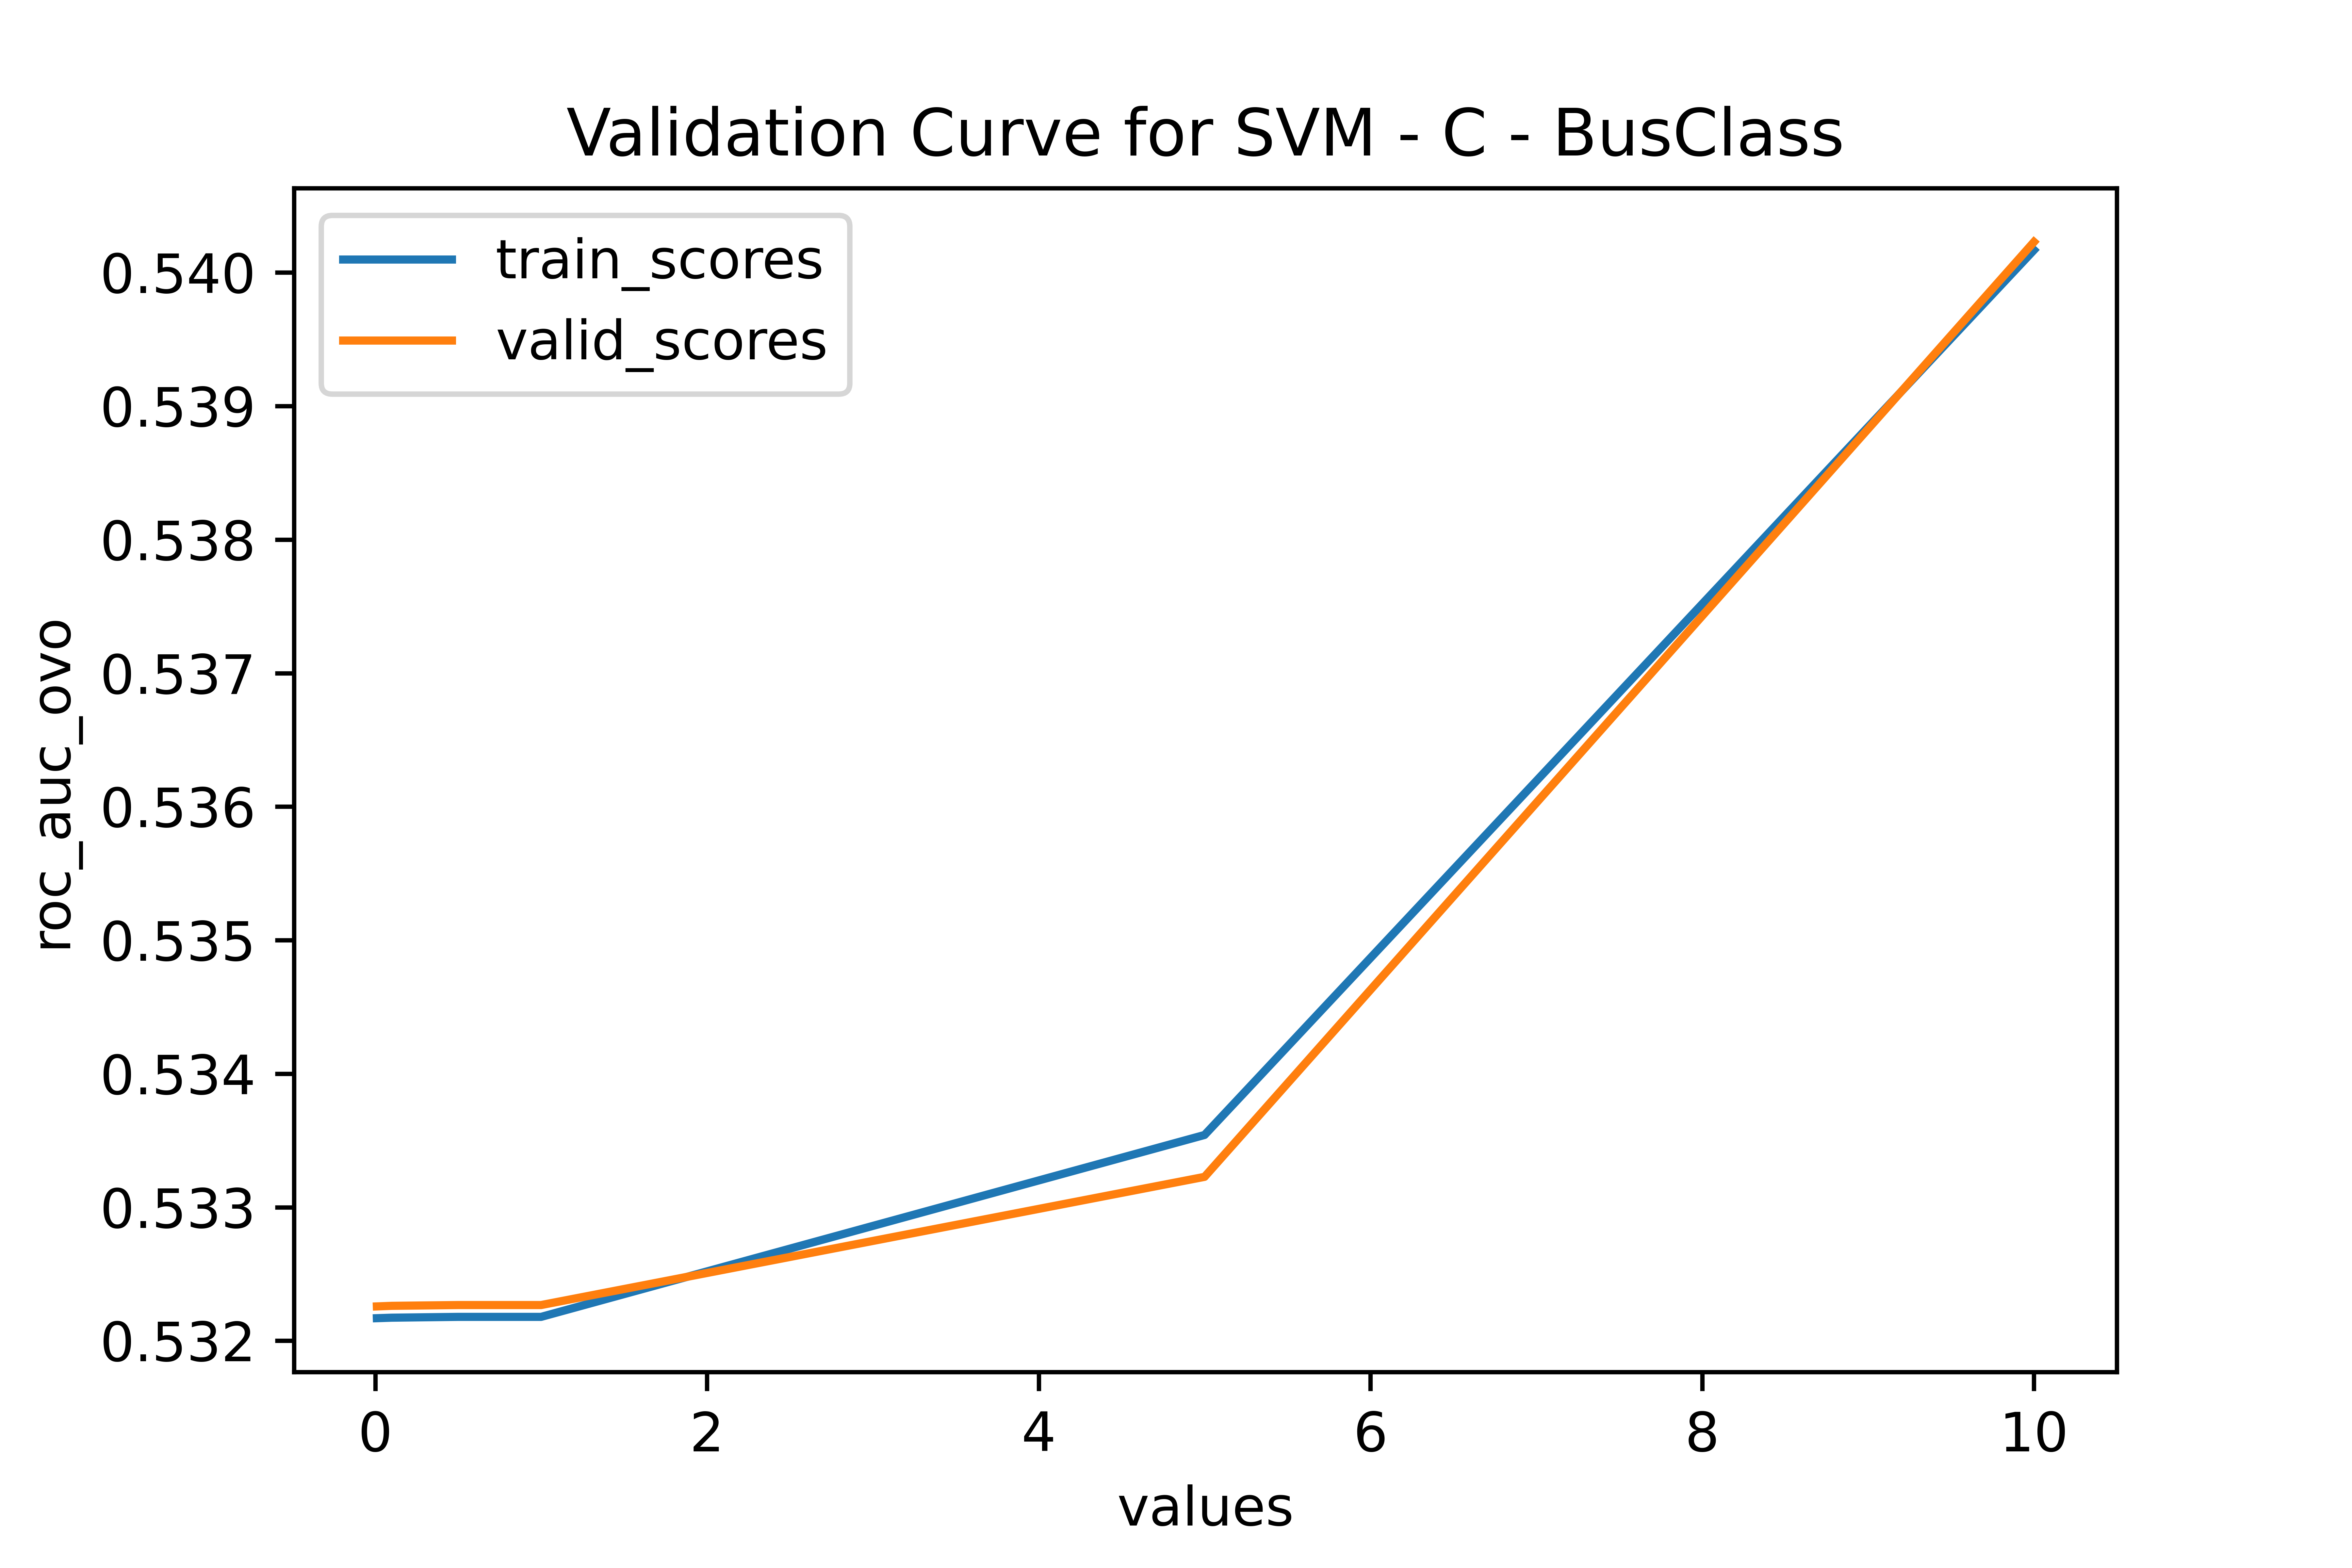
\includegraphics[width=3.4in]{Figures/BusClass-0920/SVM/val_curve_1.png}
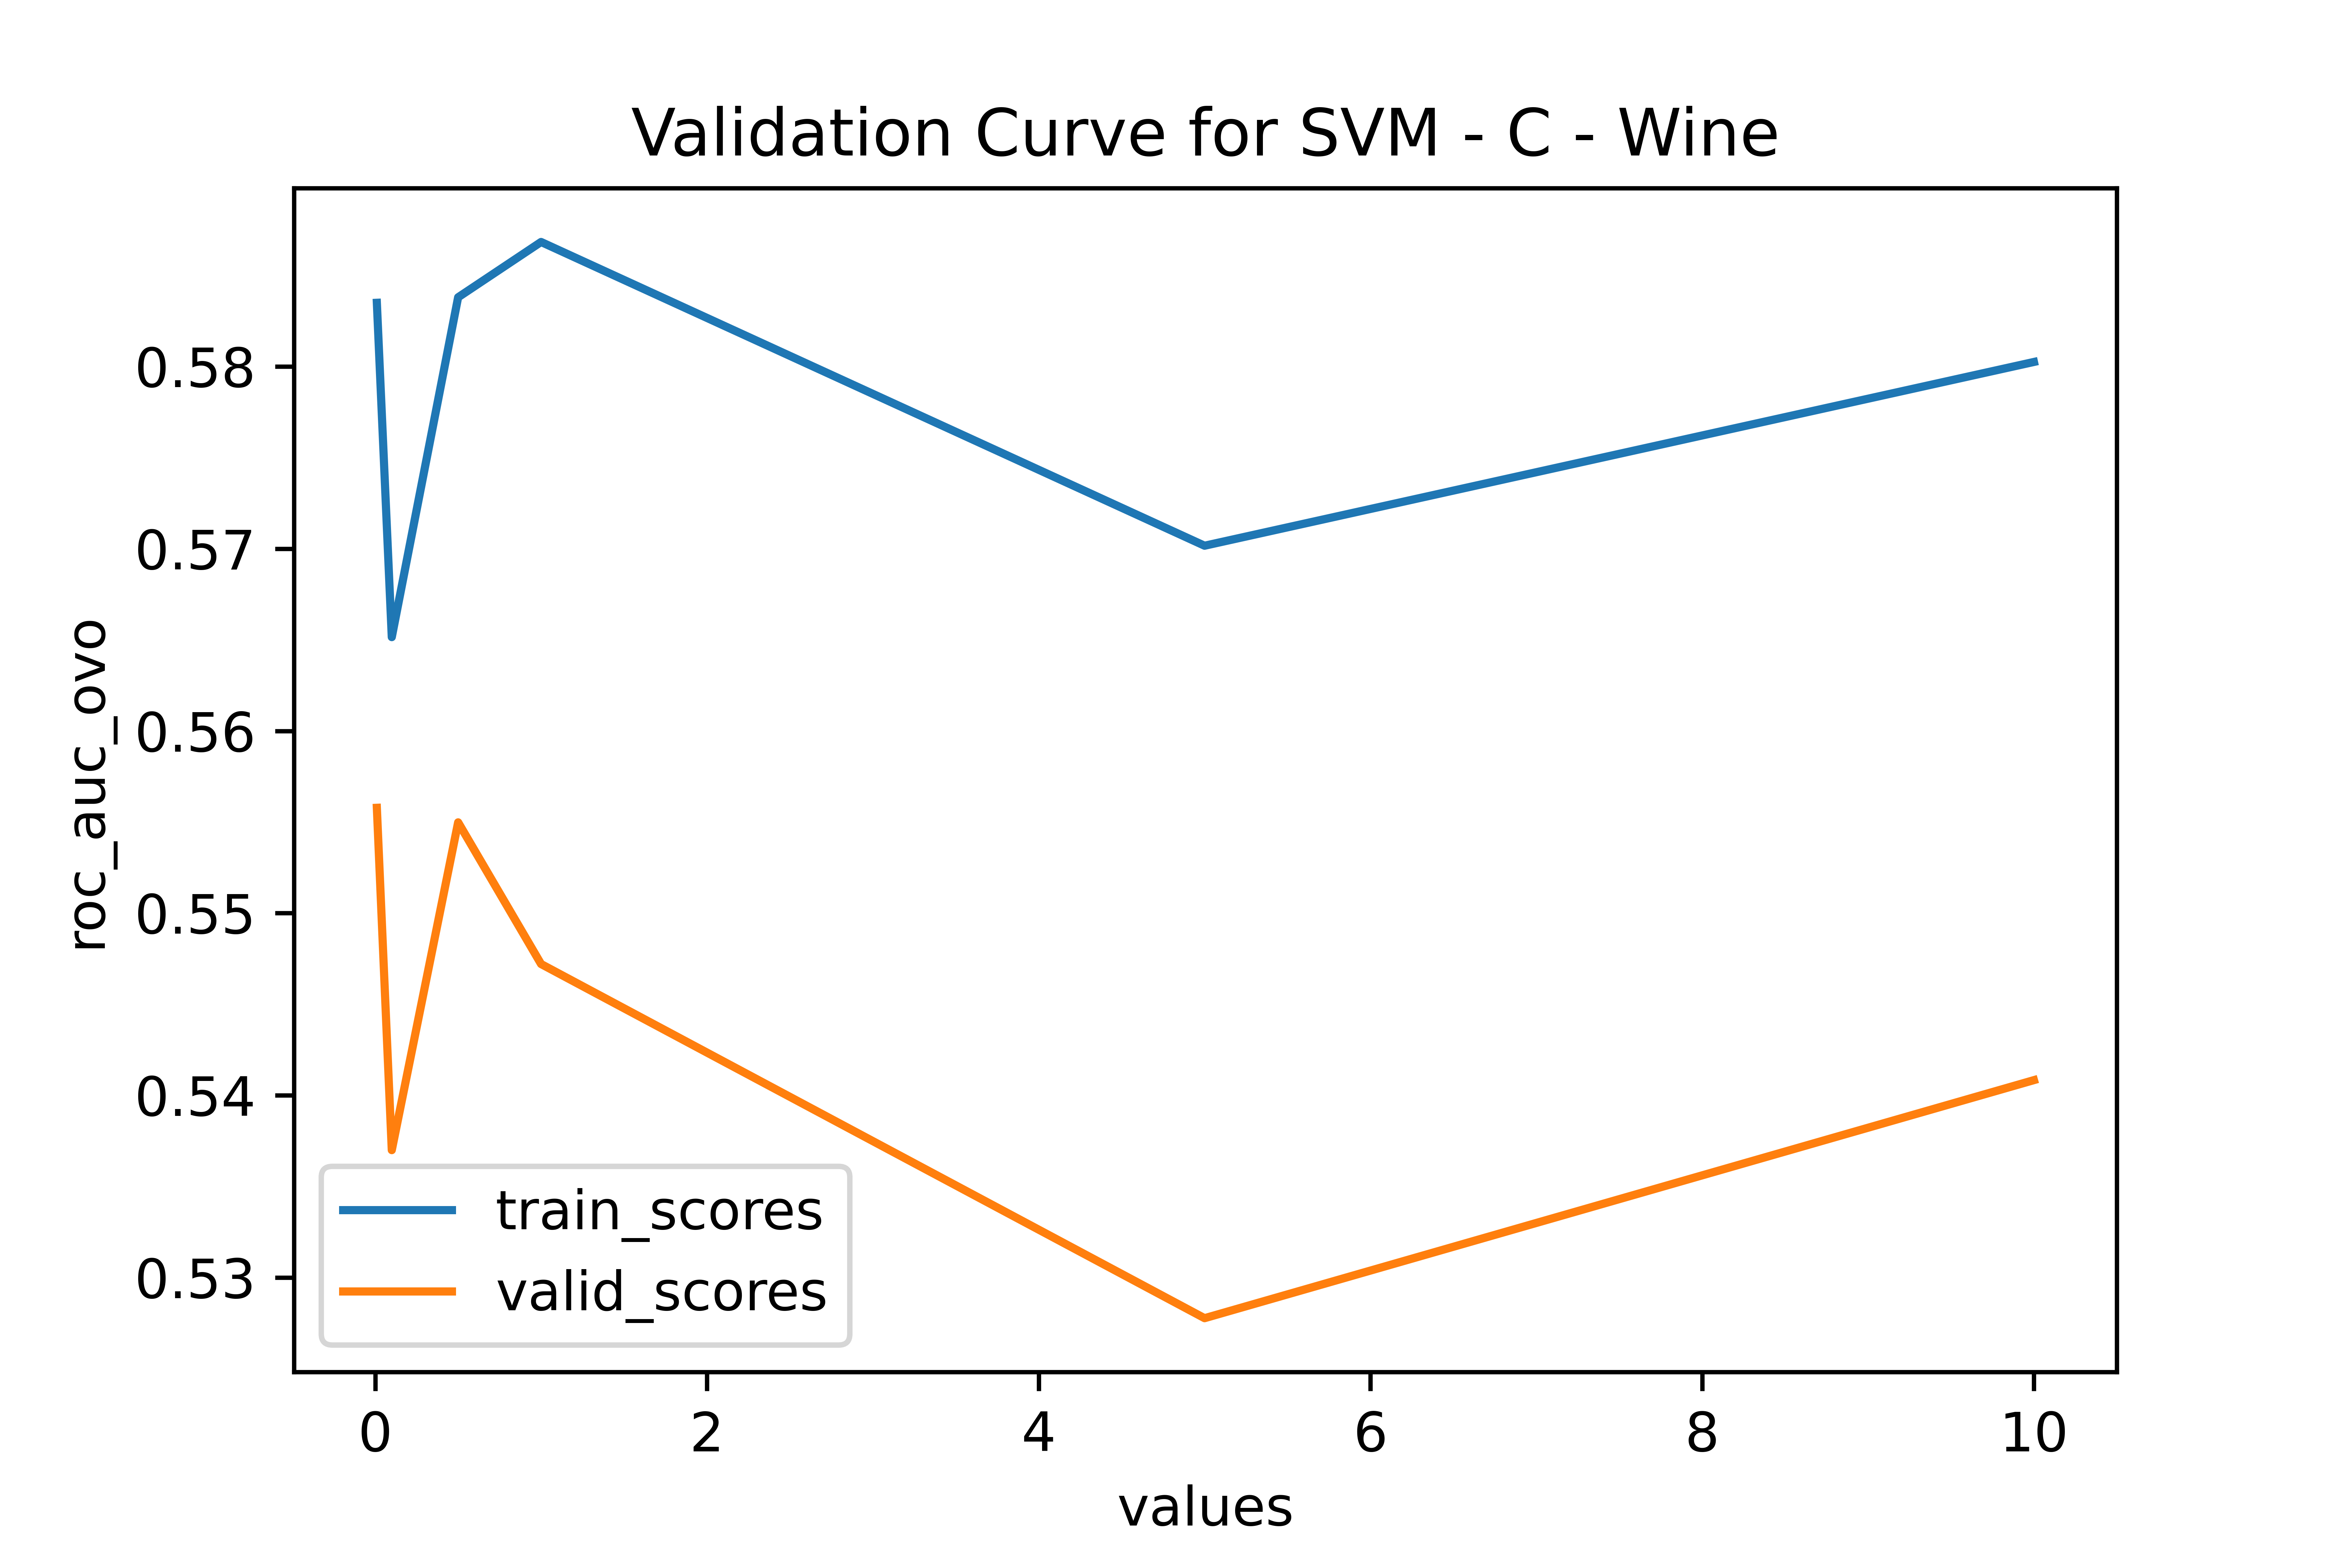
\includegraphics[width=3.4in]{Figures/Wine-0921/SVM/val_curve_1.png}

\subsubsection{Learning Curves}

Again we see that the SVMs do not exhibit stellar performance for these multi-class tasks. On the business classification dataset, we see high variance by examining the higher levels of performance on the validation data (arguably noise) that began to suffer as we added more training data. For the wine dataset, we simply never saw changes in performance on the validation data as the amount of training data increased, implying that we were never really capturing signal with our model.

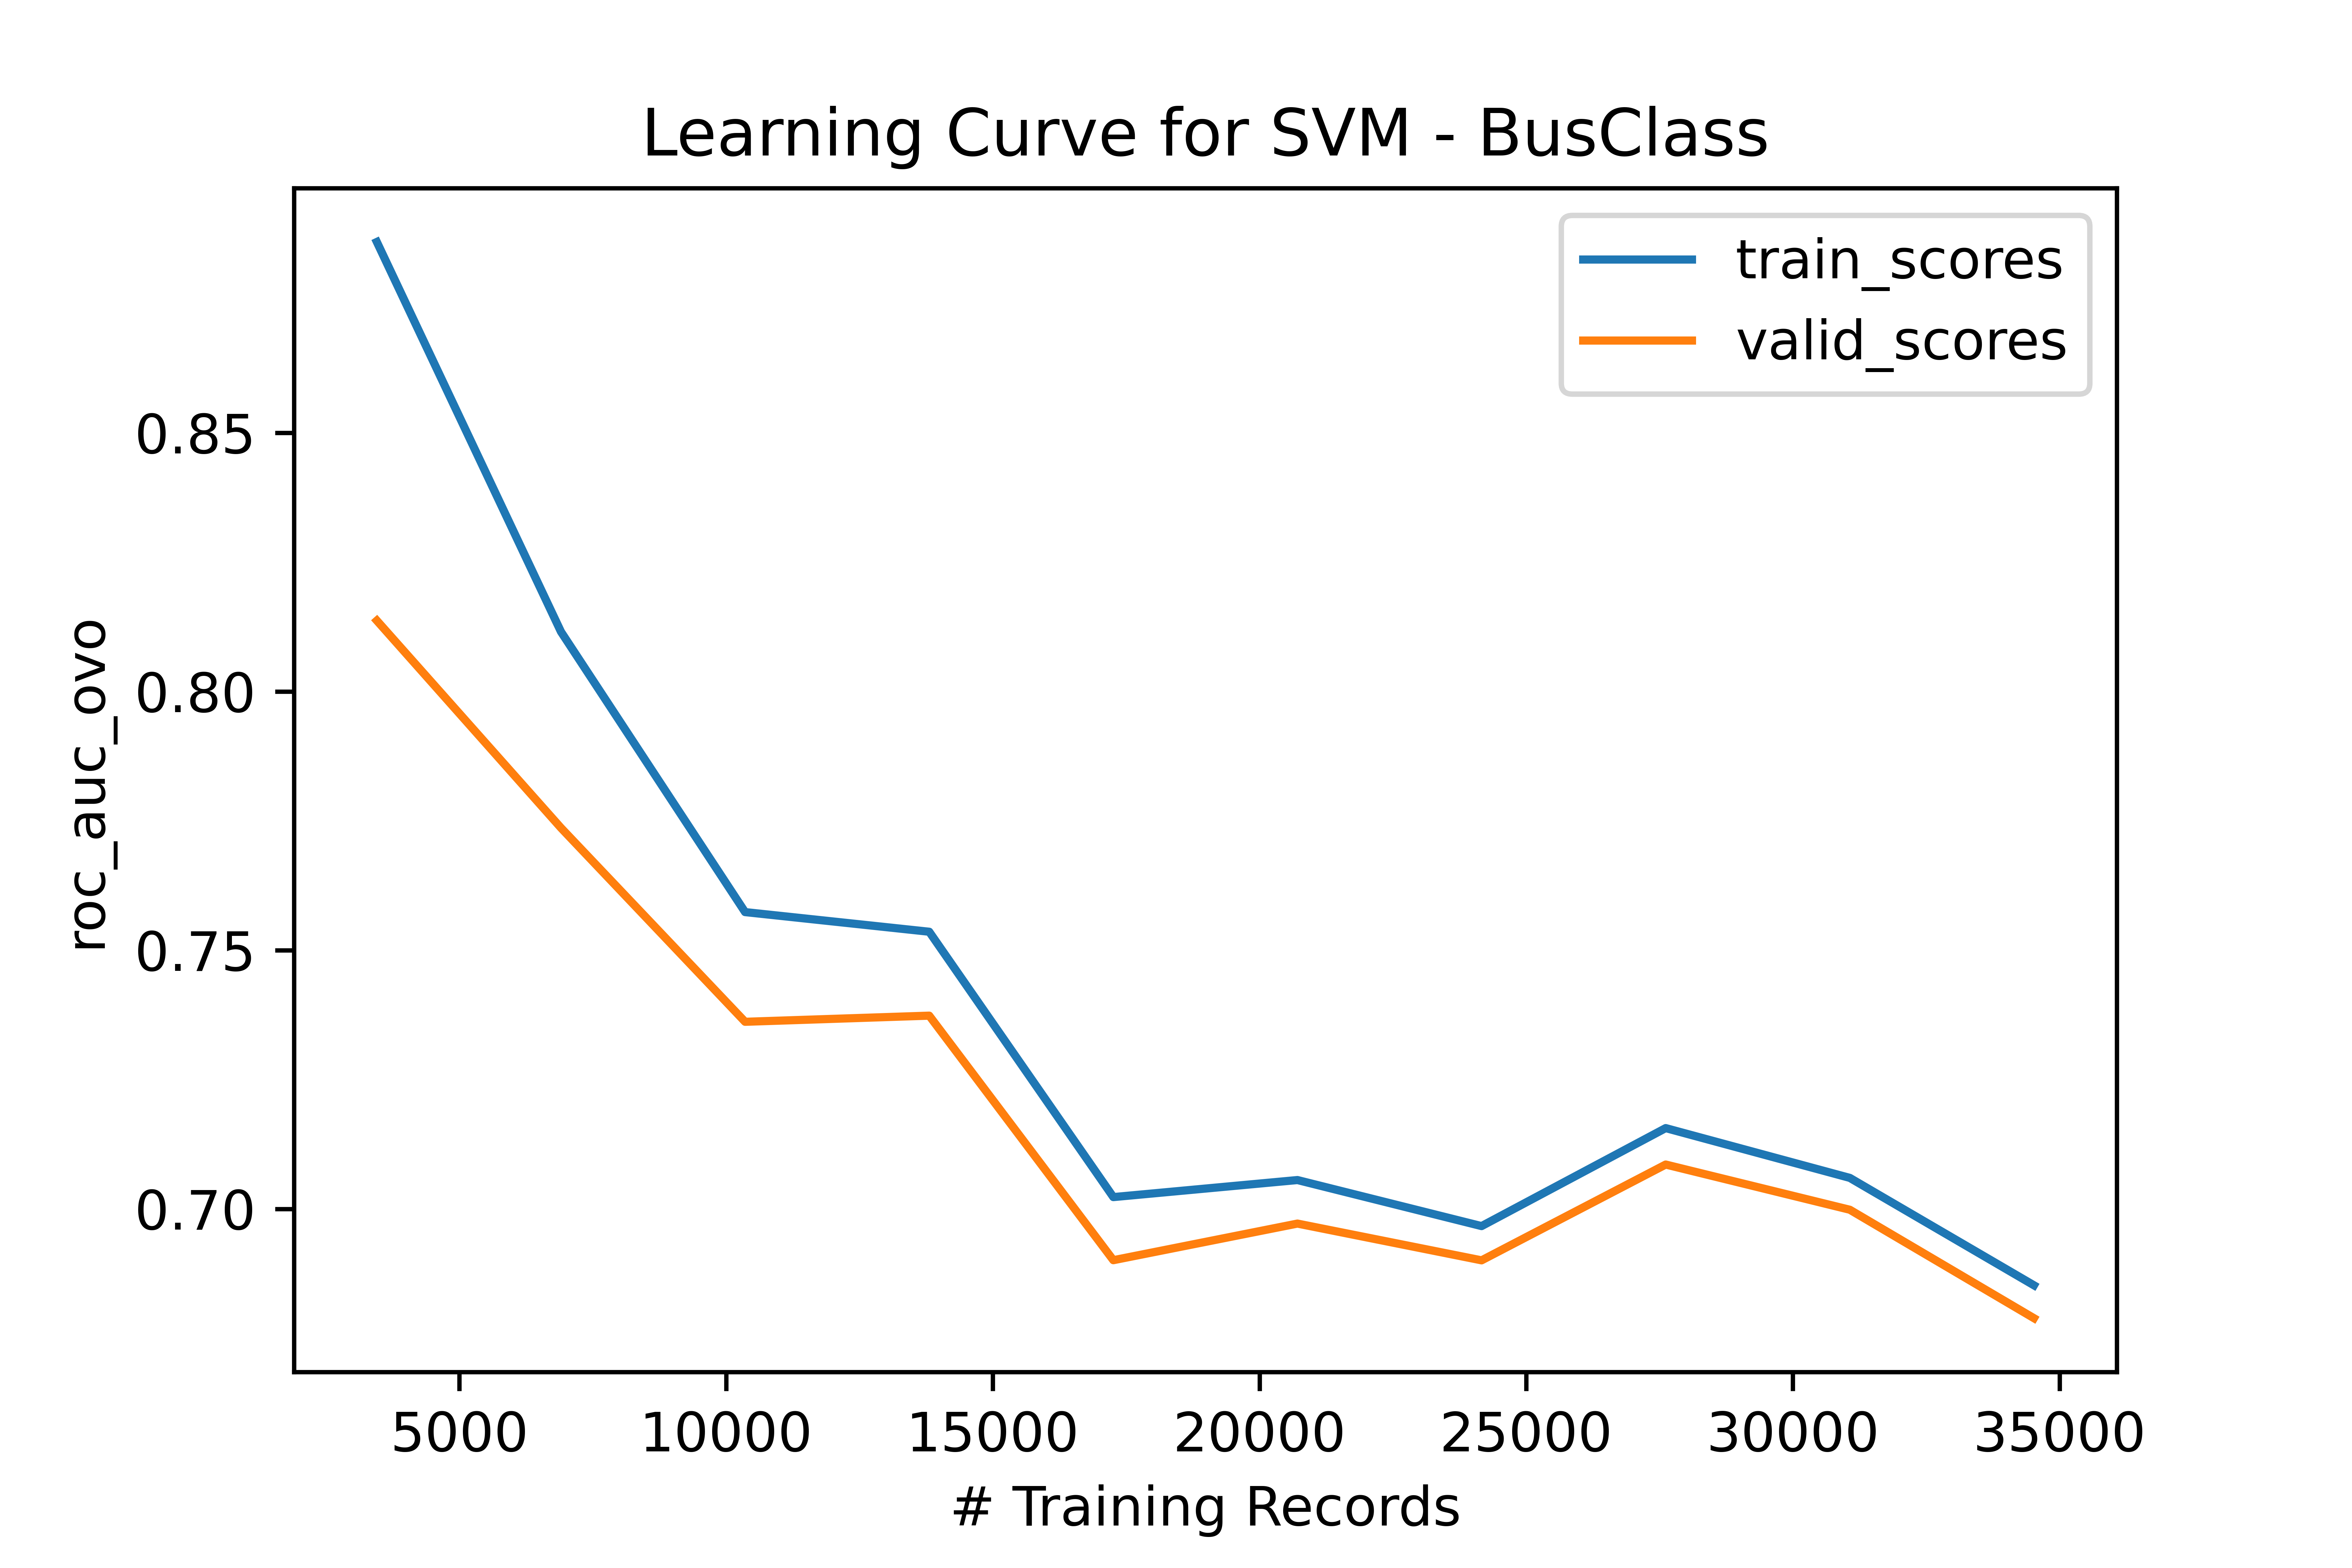
\includegraphics[width=3.4in]{Figures/BusClass-0920/SVM/learn_curve.png}
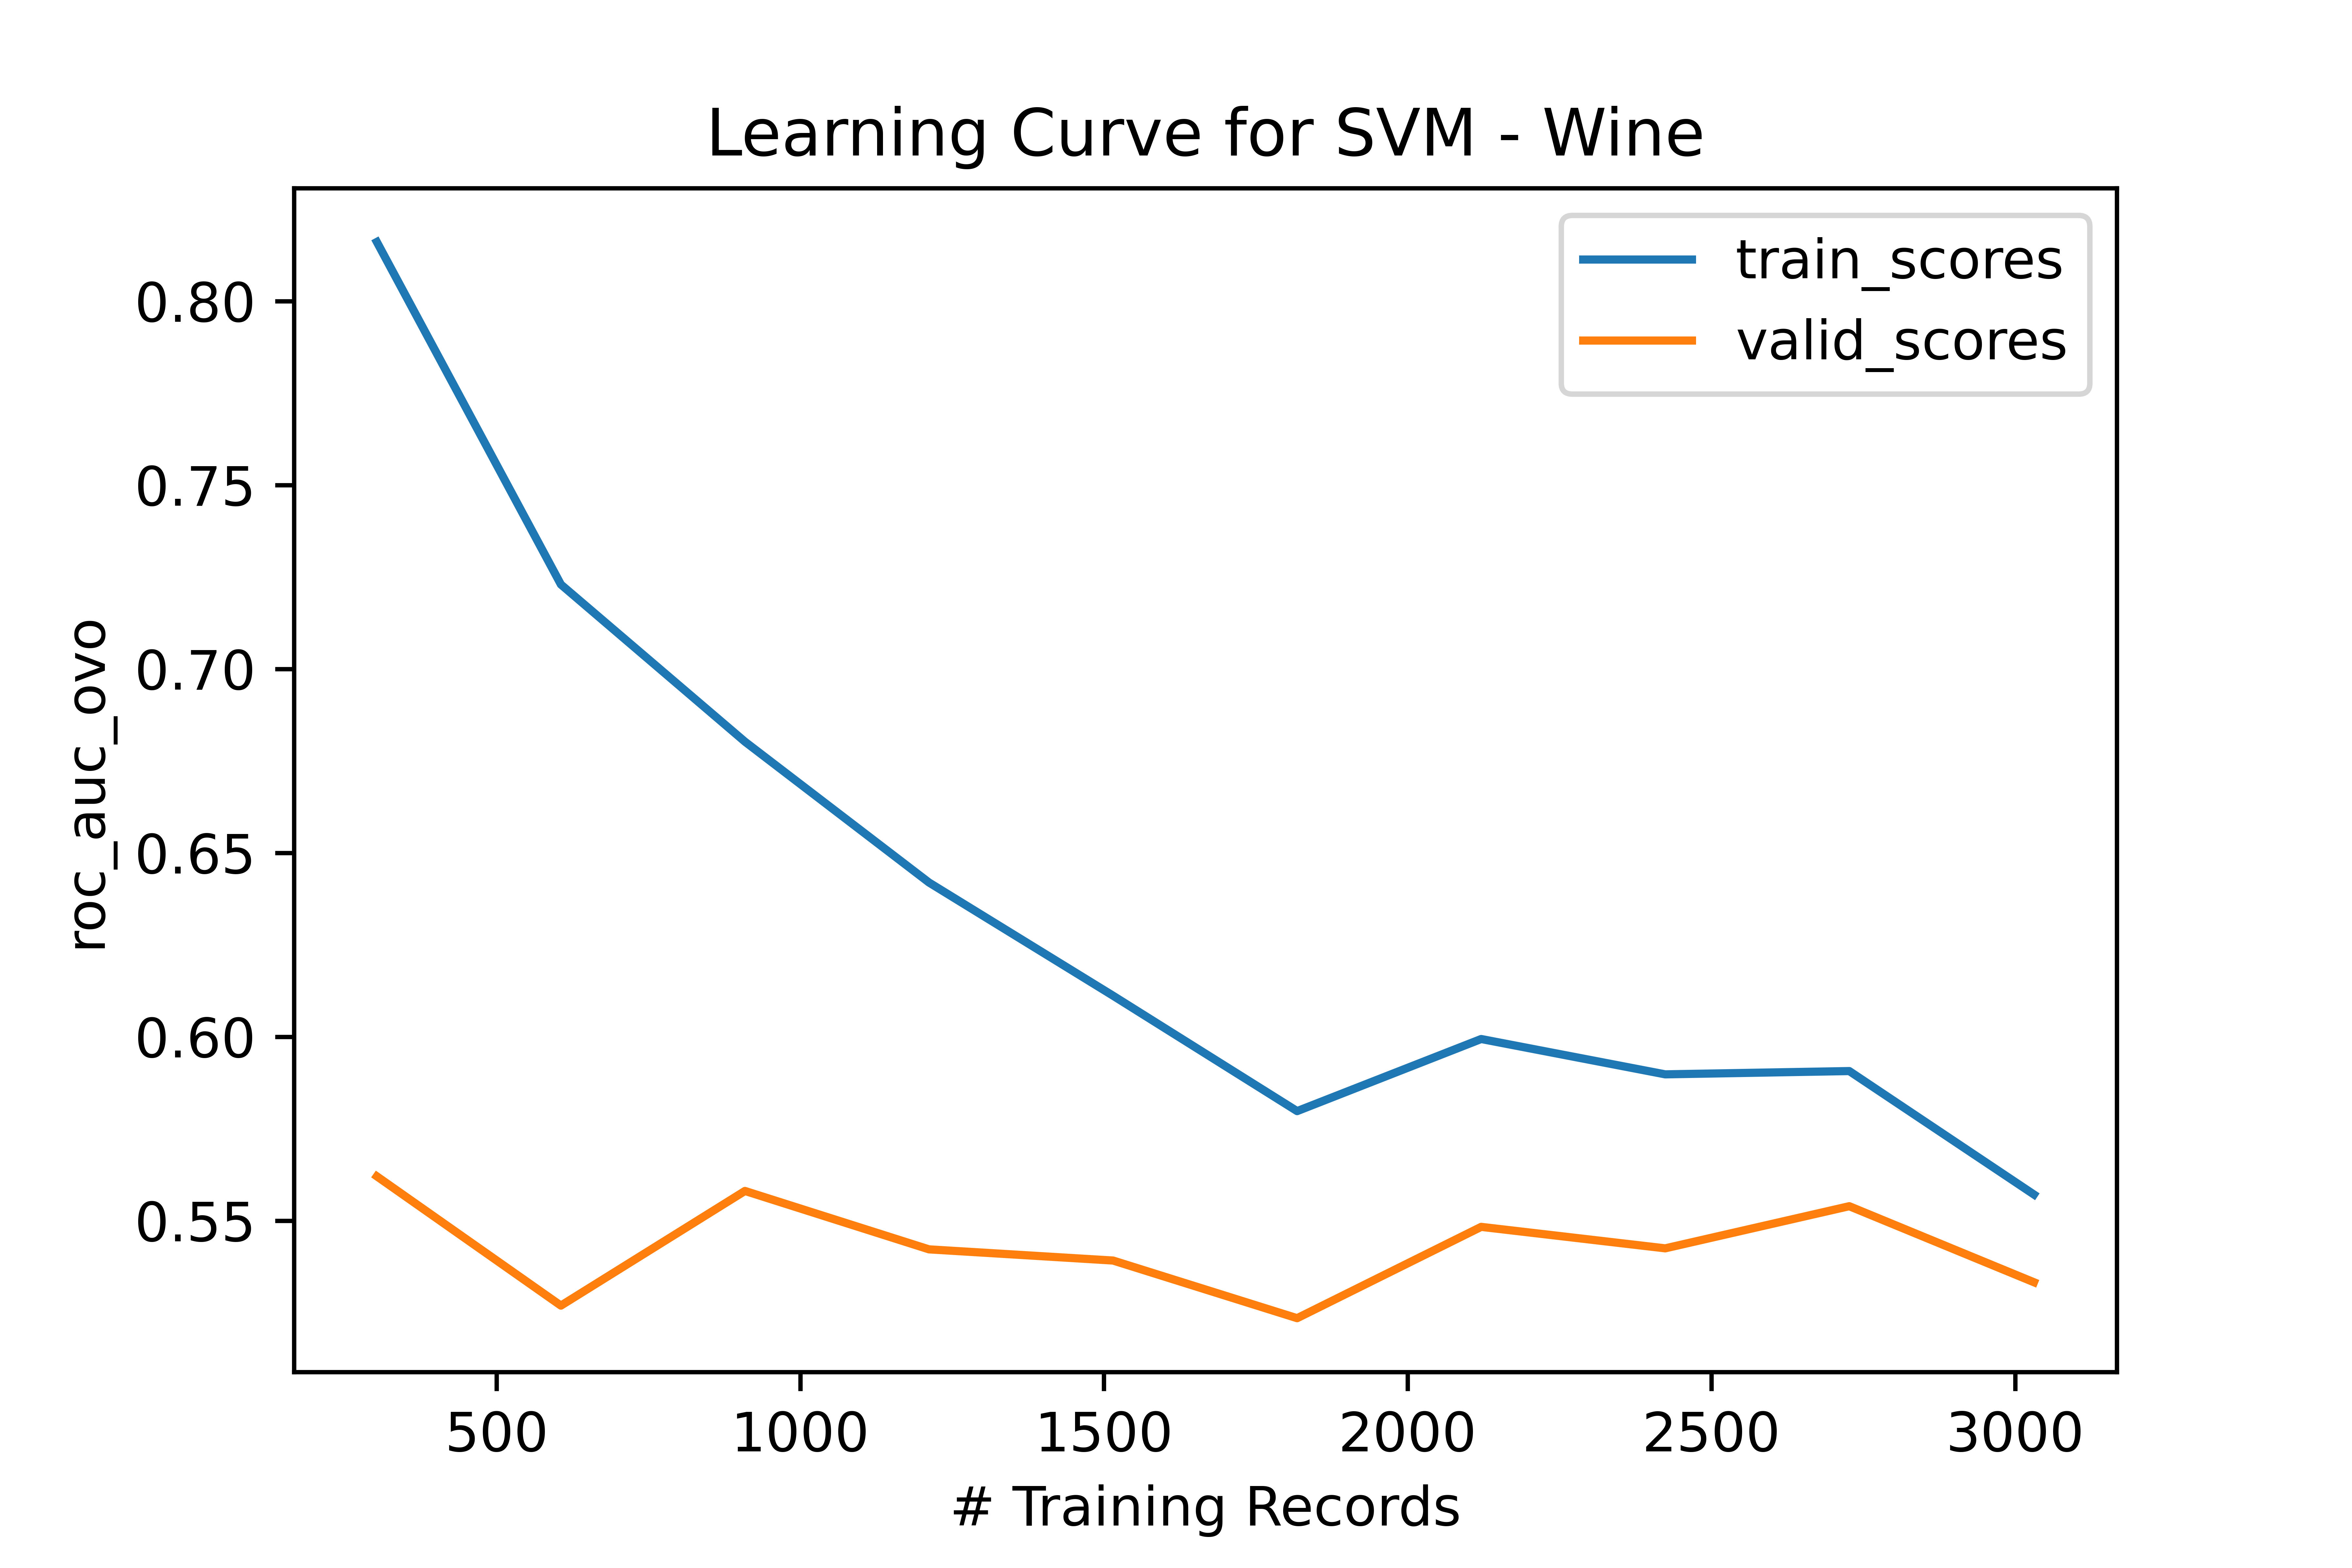
\includegraphics[width=3.4in]{Figures/Wine-0921/SVM/learn_curve.png}

\subsubsection{Wall Clock Time}
We see the familiar linear fit and near-constant predict times for this algorithm and these datasets. Again, the main difference is the magnitude of times, not the shape of the graphs.

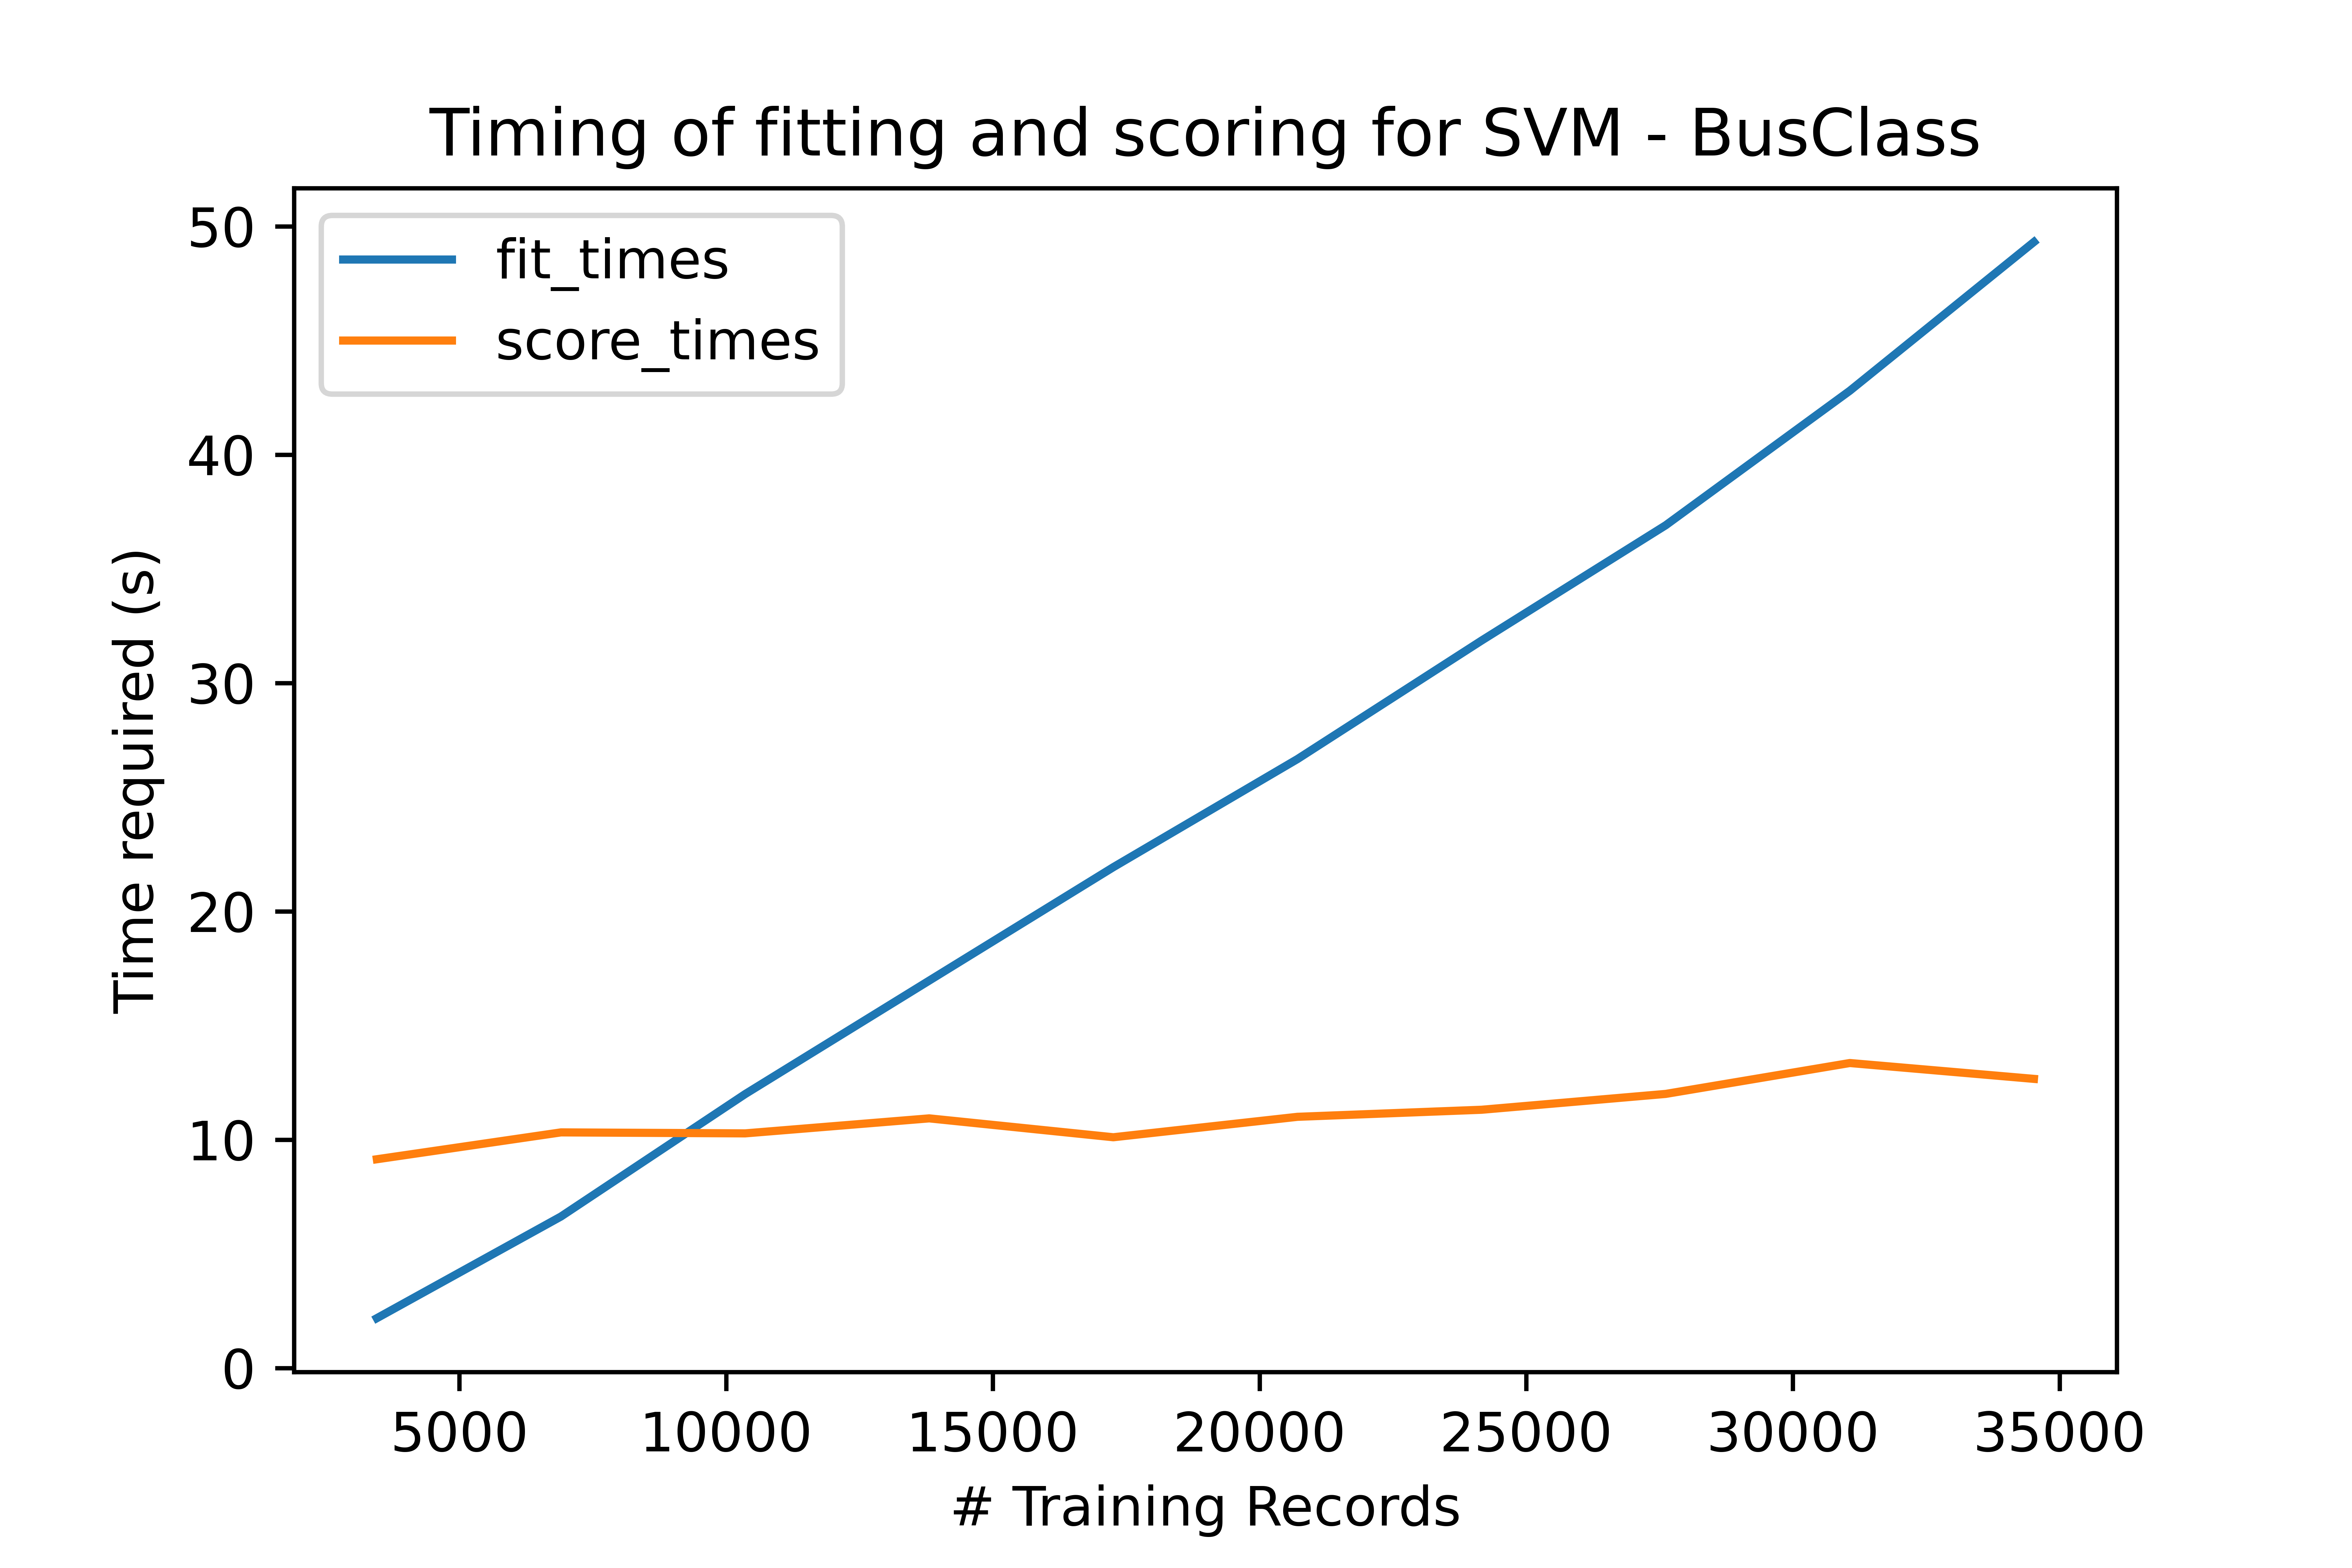
\includegraphics[width=3.4in]{Figures/BusClass-0920/SVM/time_curve.png}
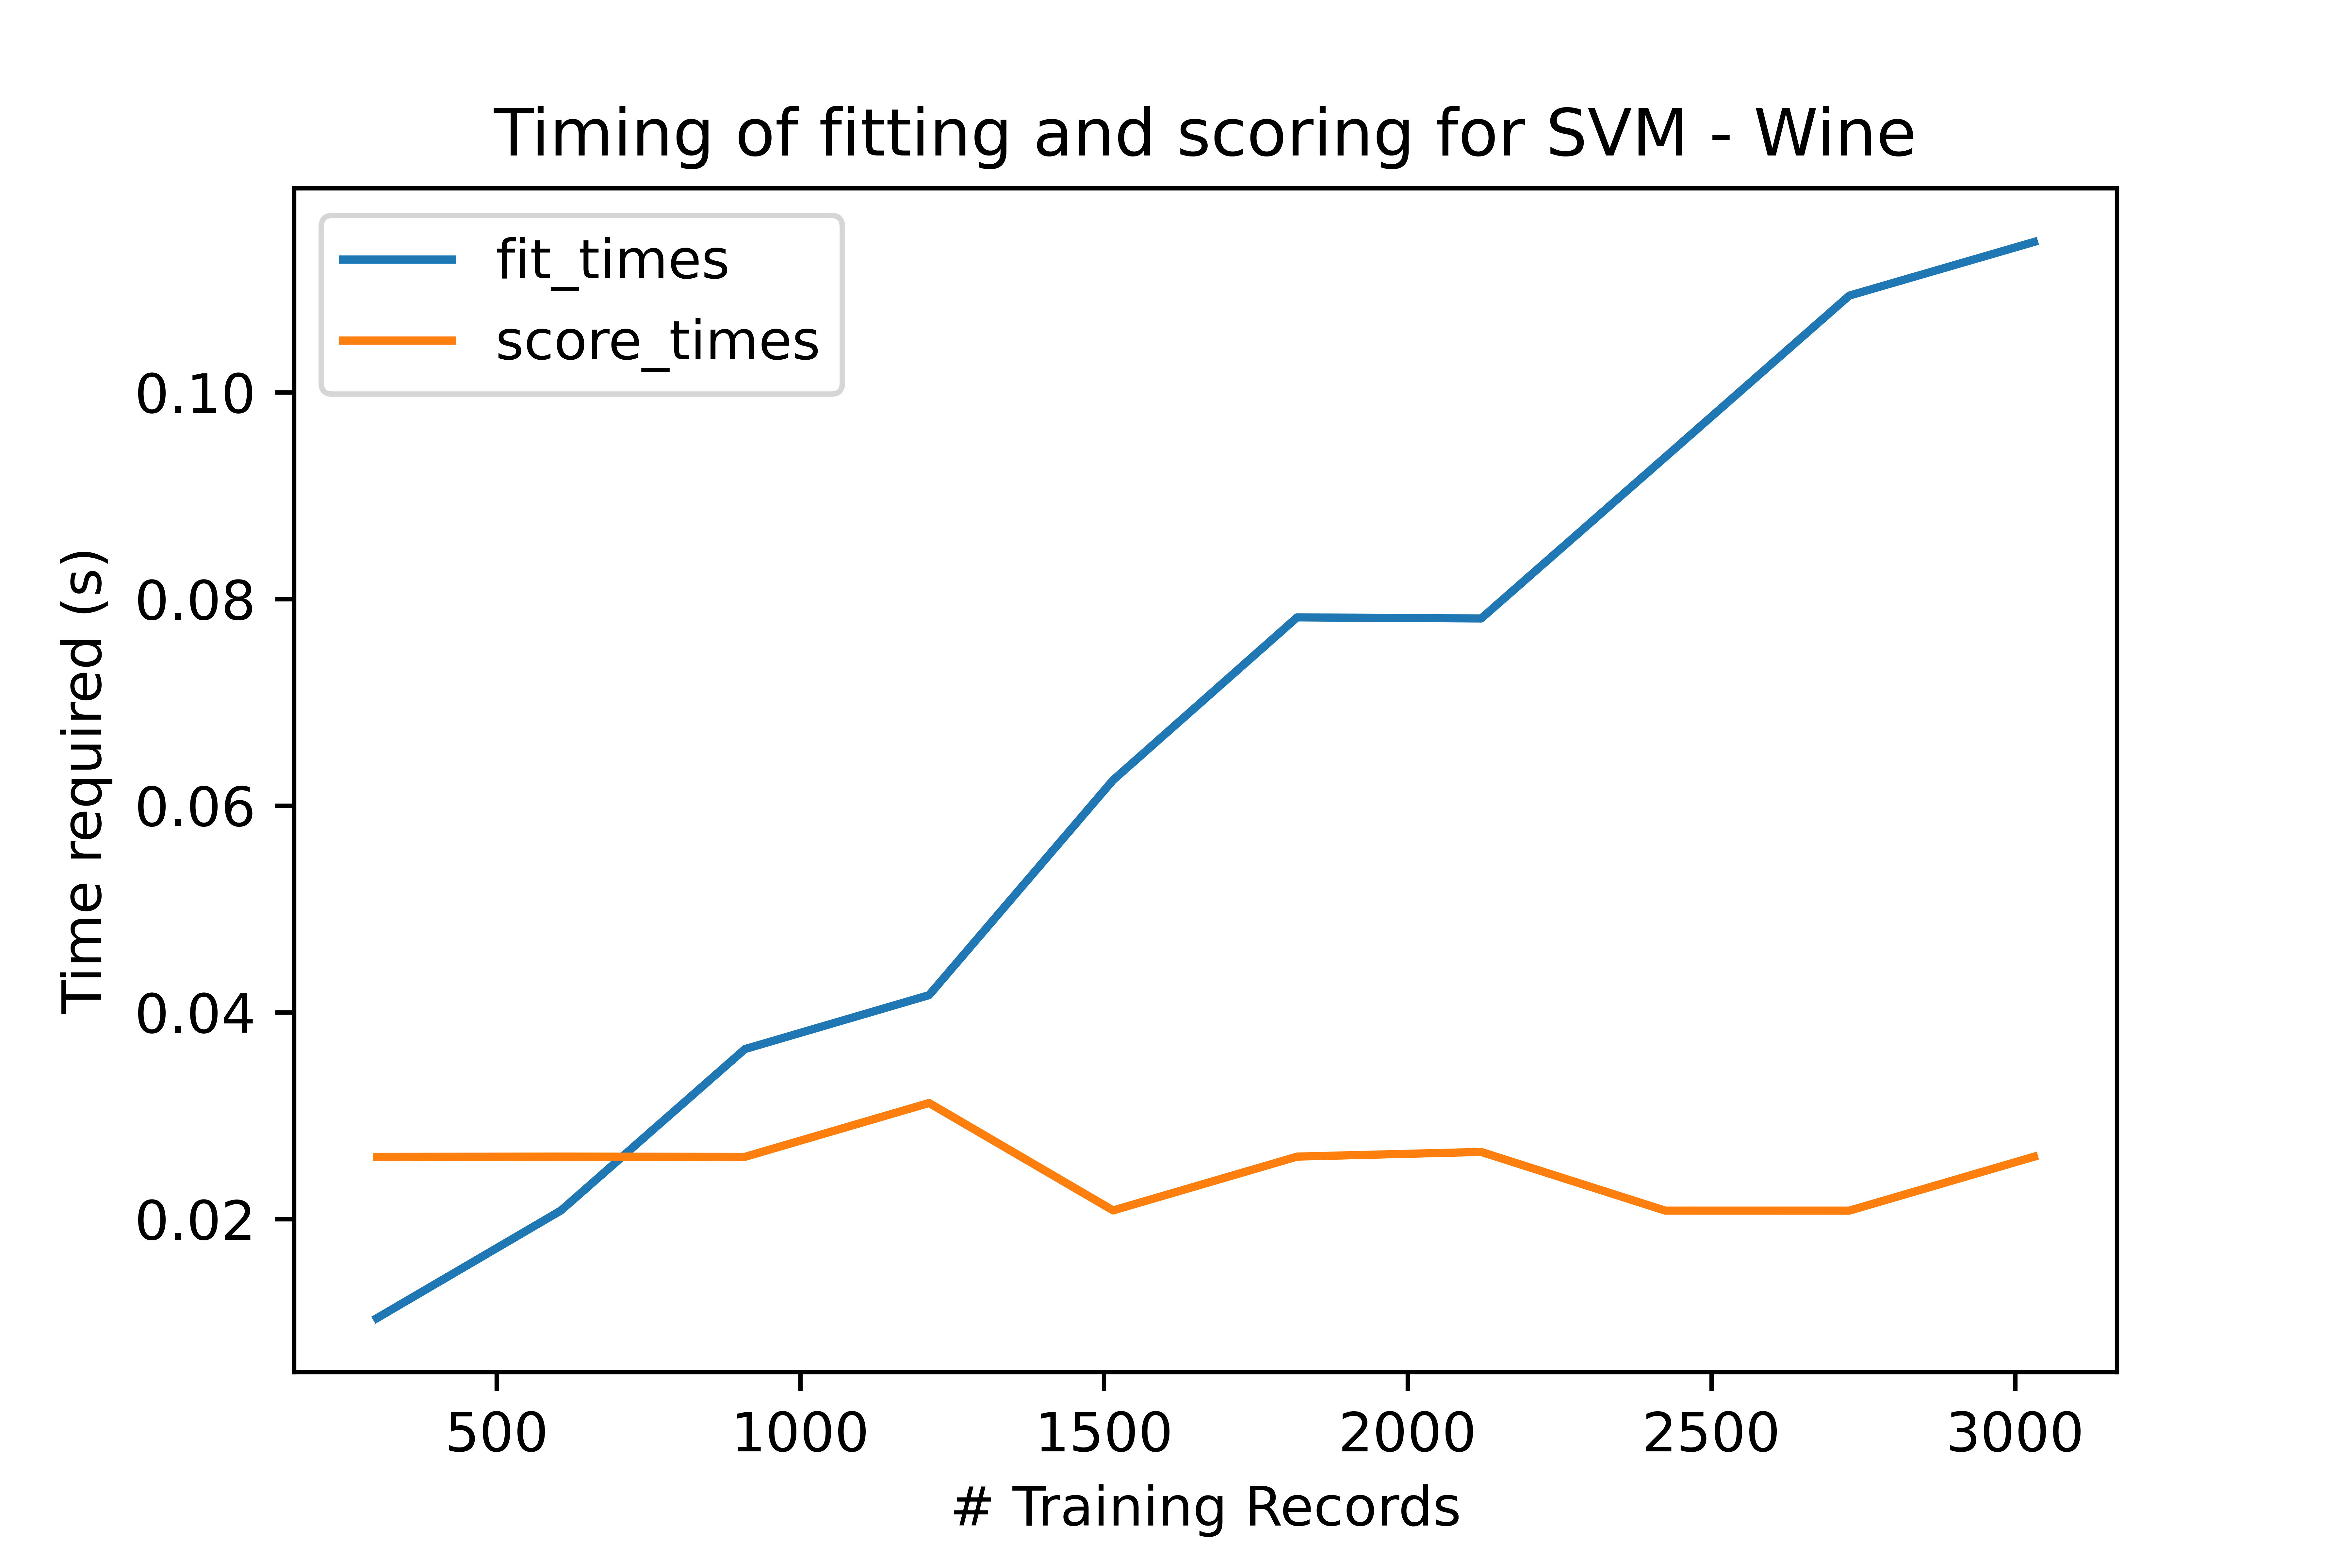
\includegraphics[width=3.4in]{Figures/Wine-0921/SVM/time_curve.png}


\subsection{k-Nearest Neighbors}

\subsubsection{Hyperparameter Tuning}

When it comes to selecting the right amount of neighbors, we see a similar contrast as observed with the decision tree's max depth parameter. It appears that we require substantially more neighbors to get the right classification for the business classification task than for the wine model, which only requires 5. I believe this is largely due to the substantial differences in width of each of these datasets, as more information is encoded in each feature of the wine dataset. We also see that weighted distances are generally better than uniform weights for the nearest neighbors, futher emphasizing the importance of the distance metric.

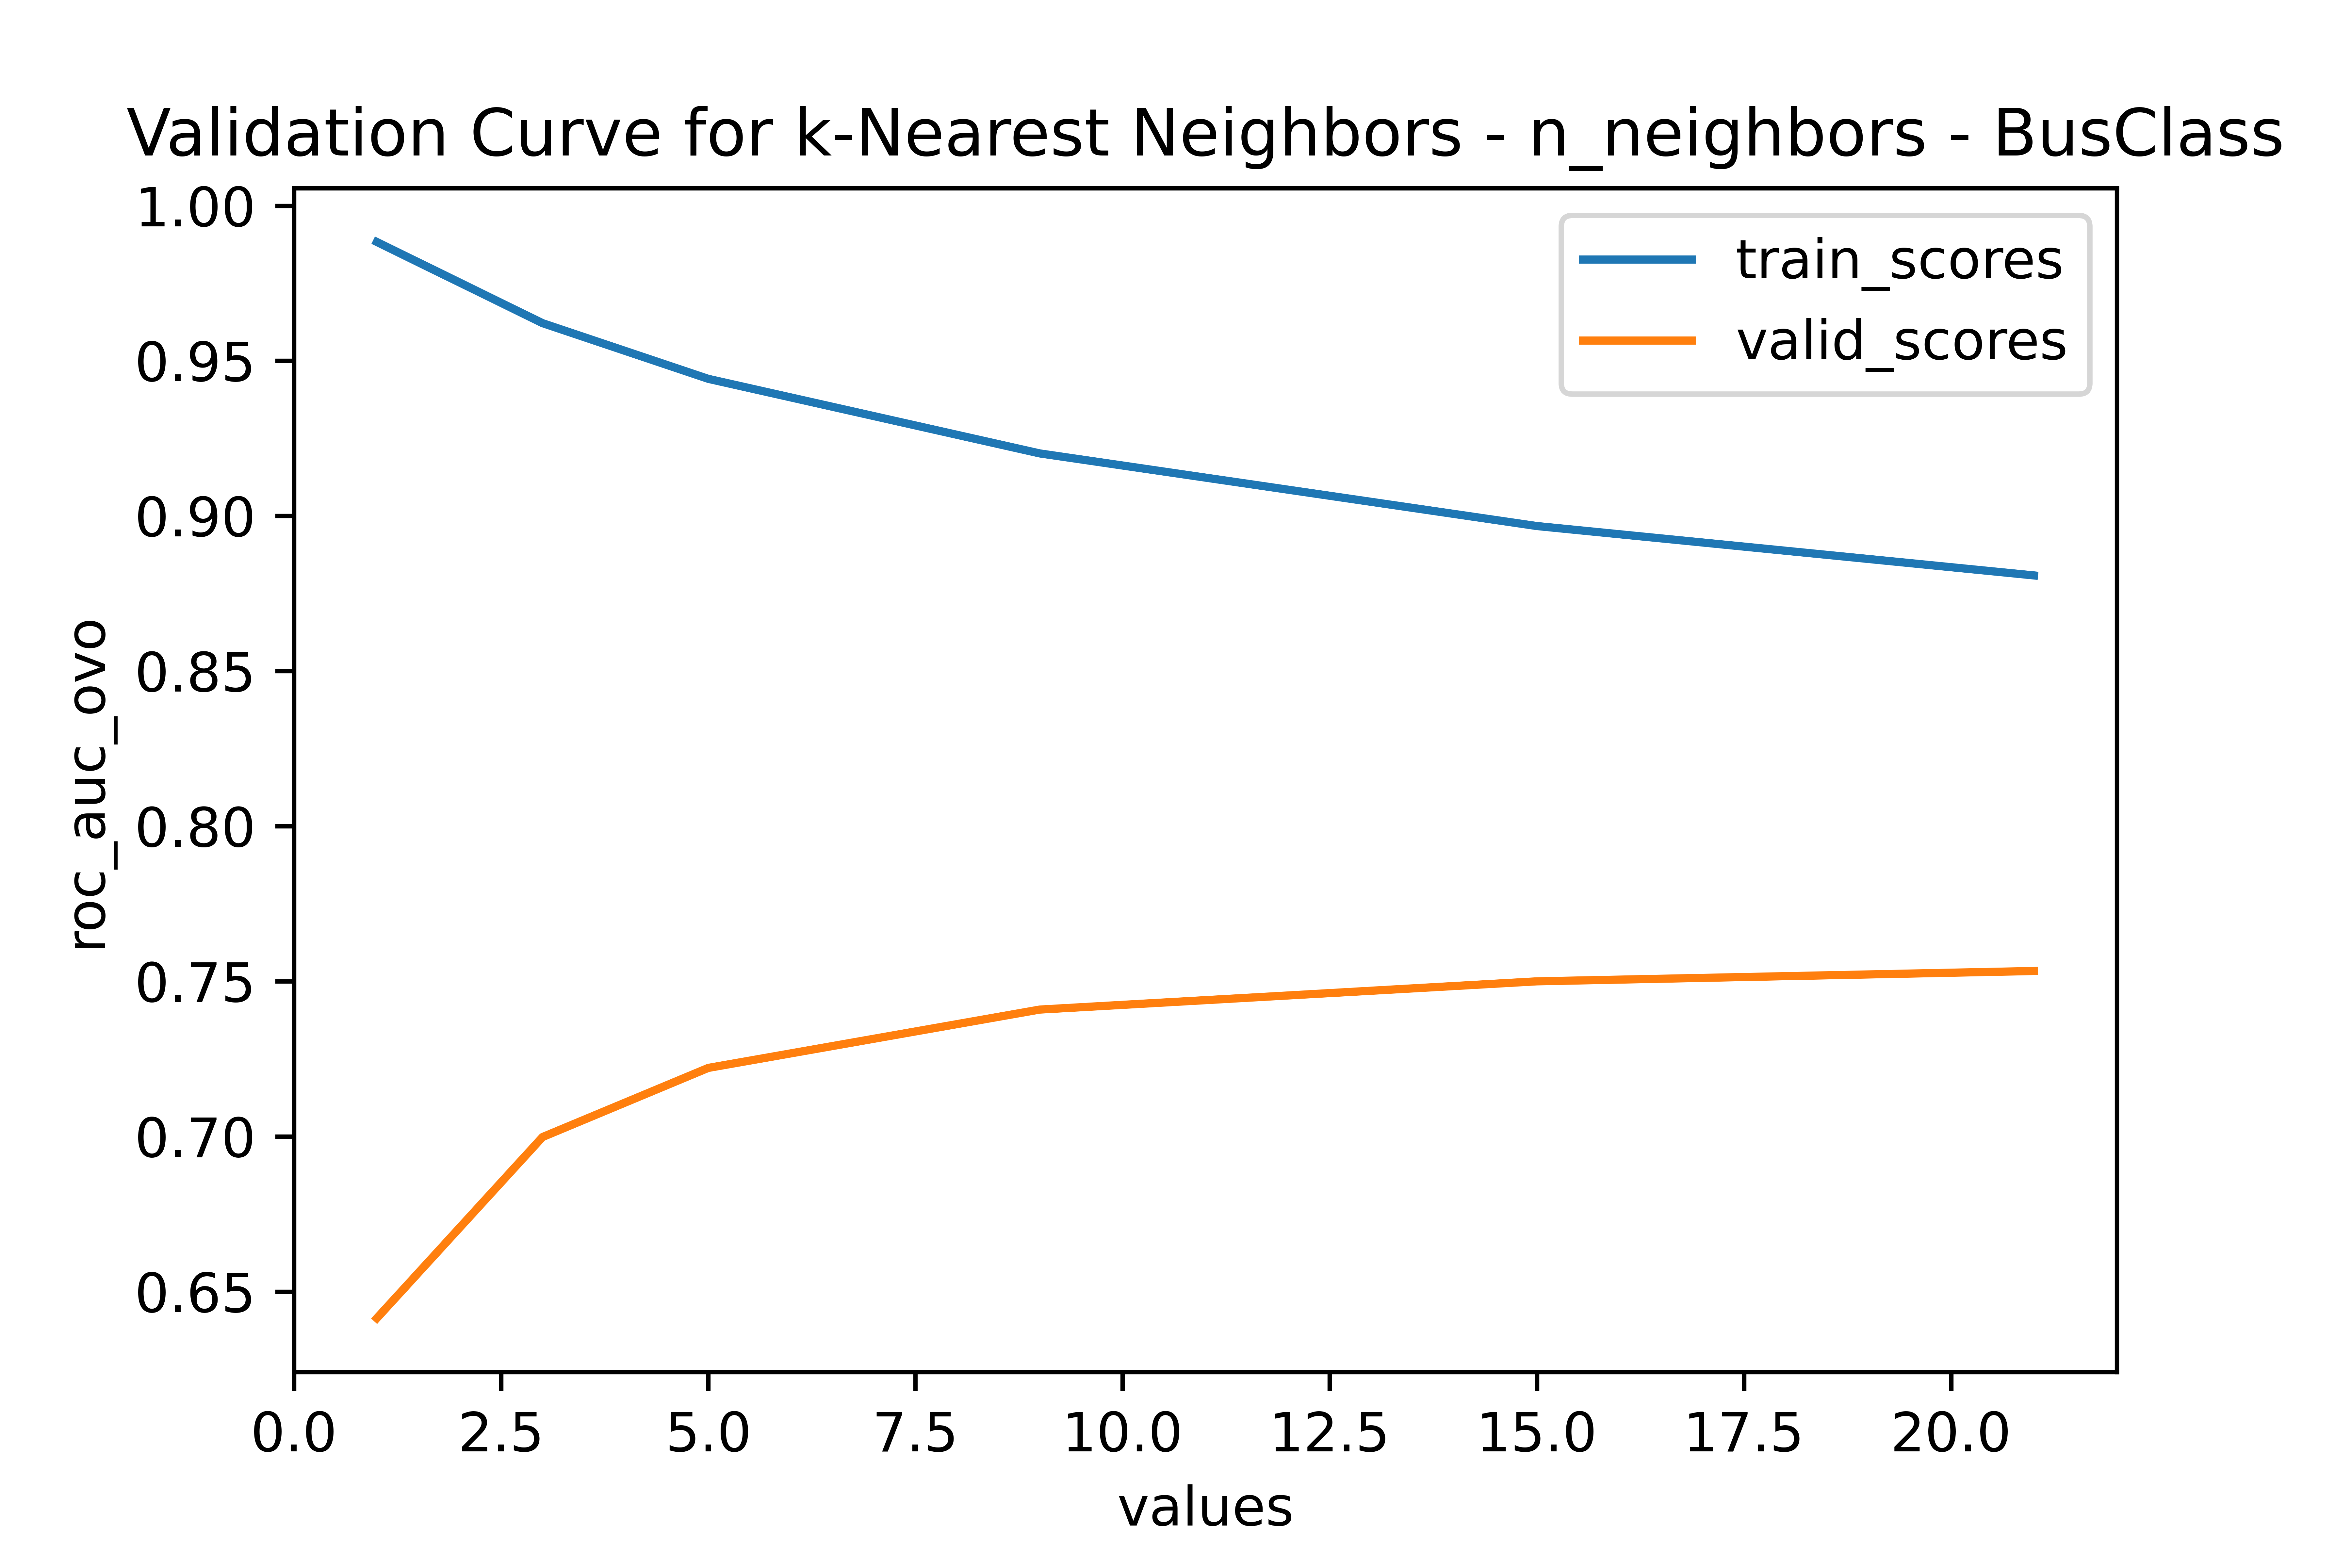
\includegraphics[width=3.4in]{Figures/BusClass-0920/KNN/val_curve_0.png}
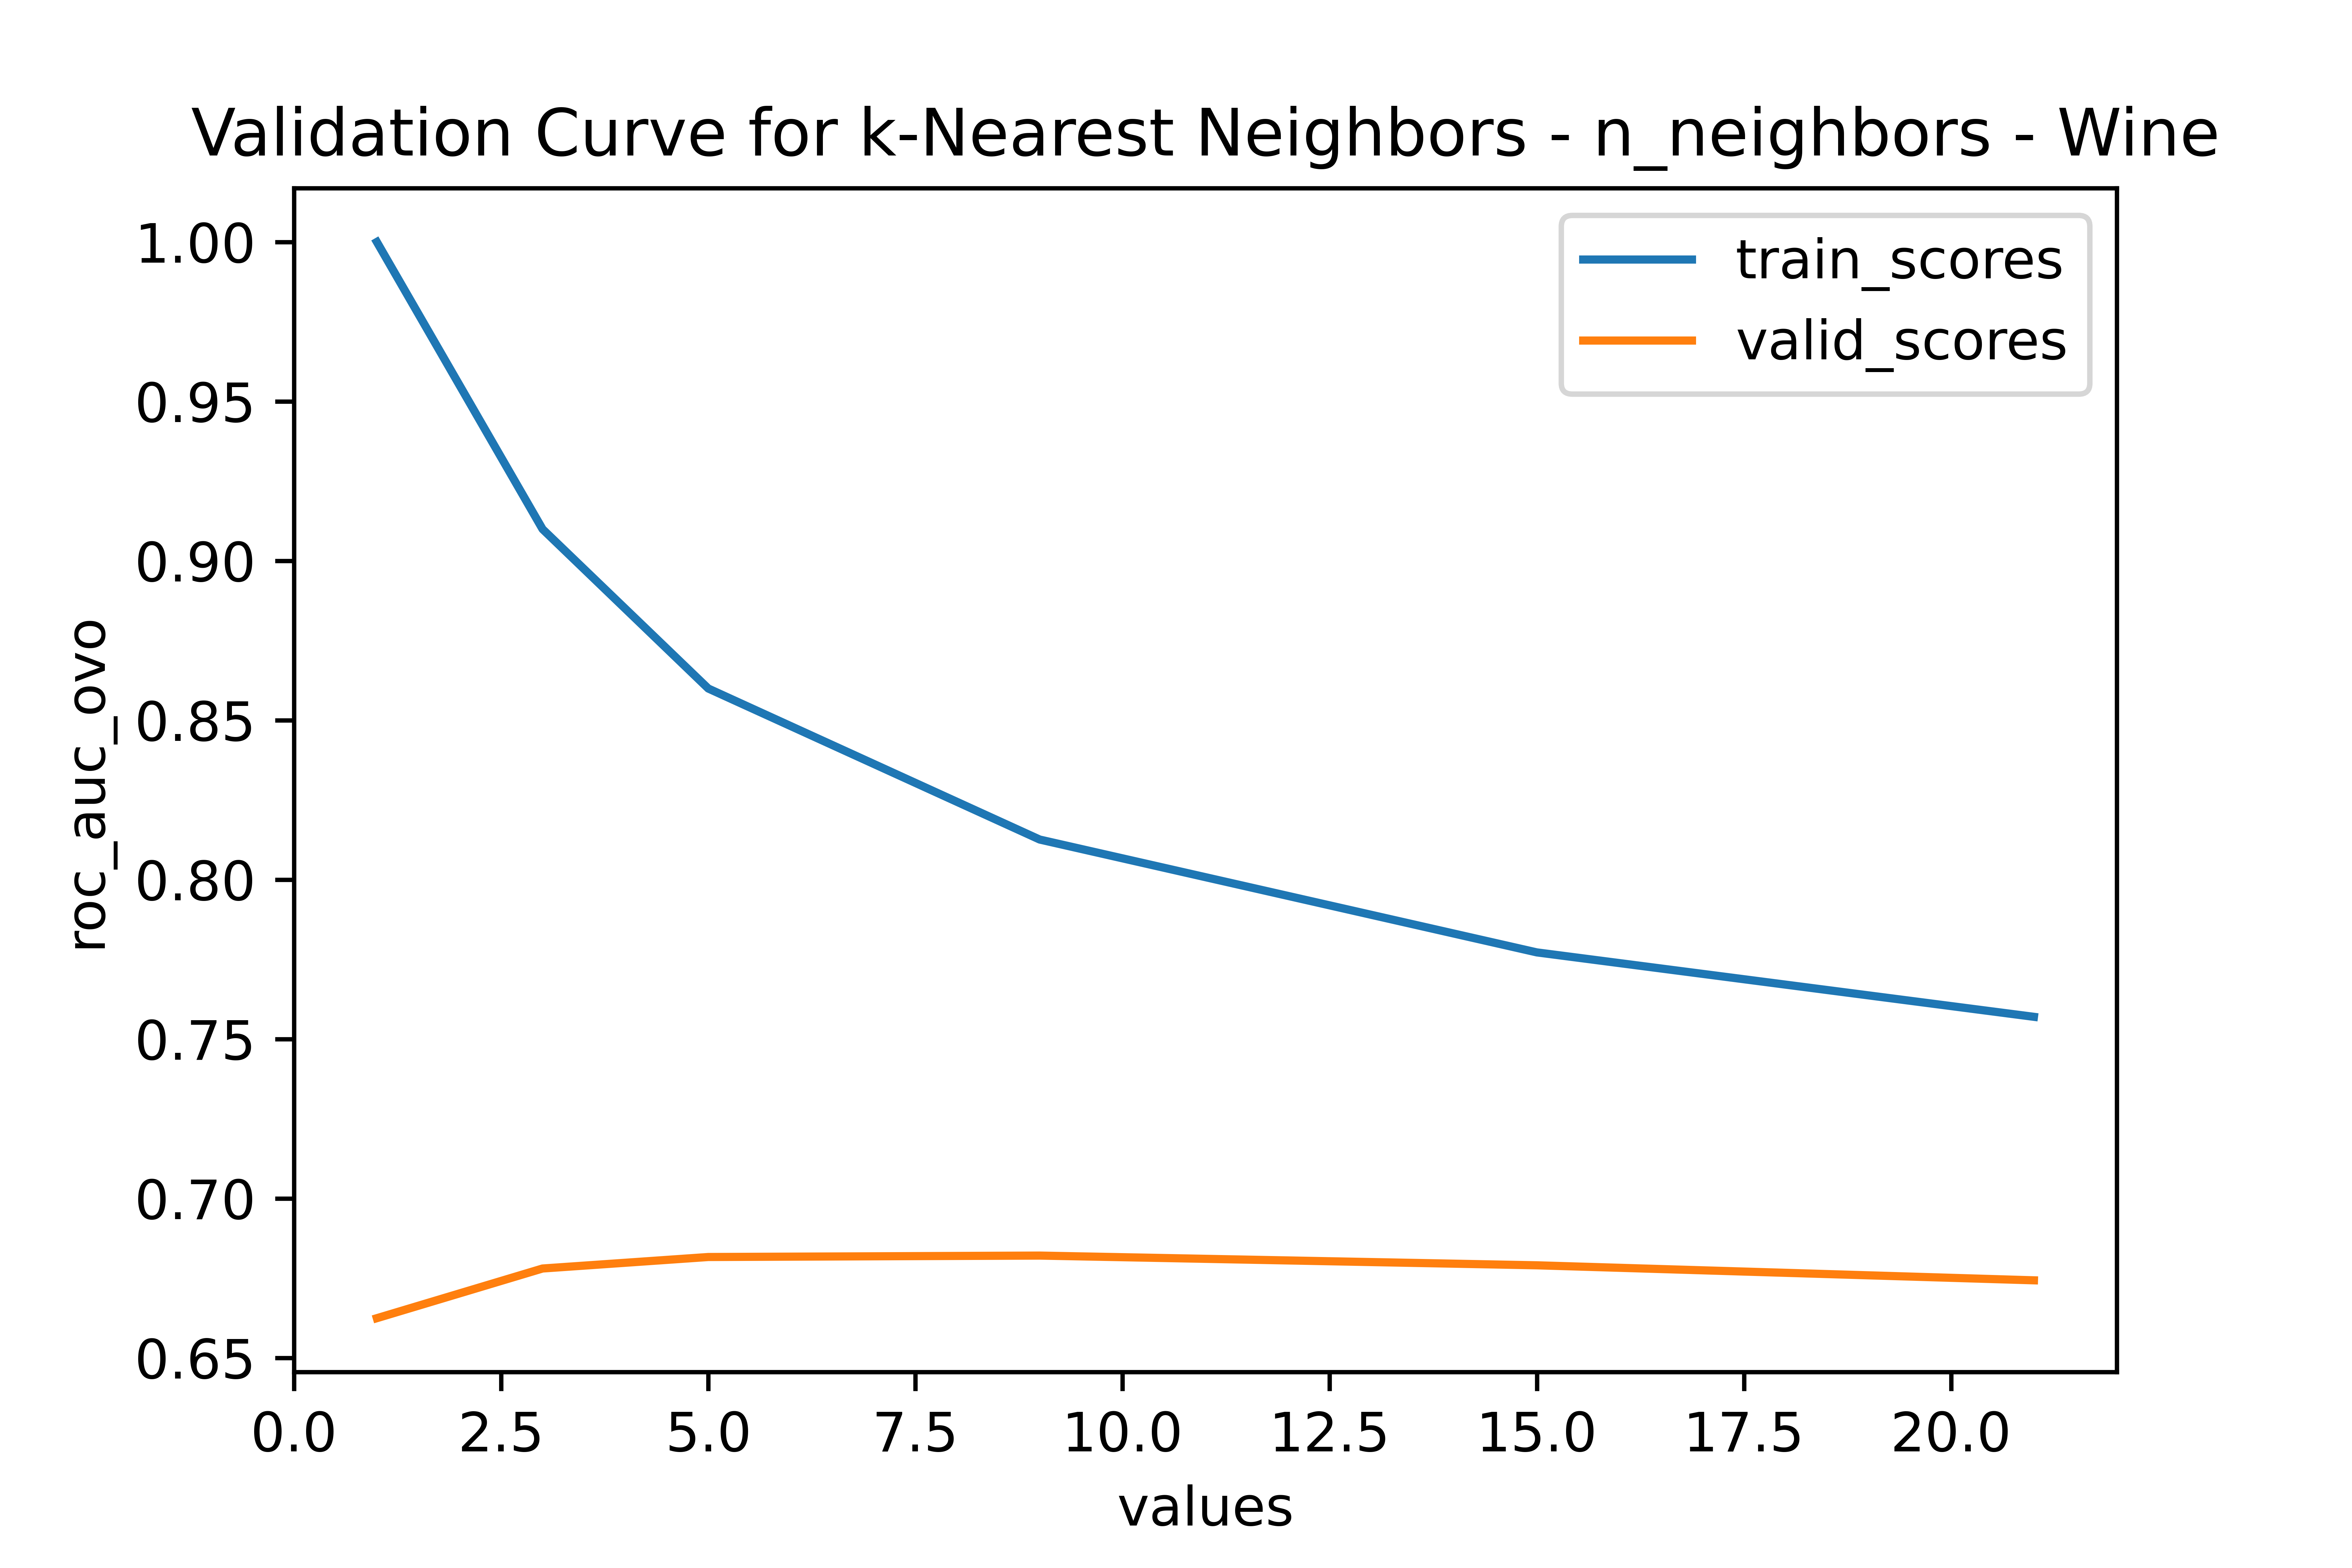
\includegraphics[width=3.4in]{Figures/Wine-0921/KNN/val_curve_0.png}
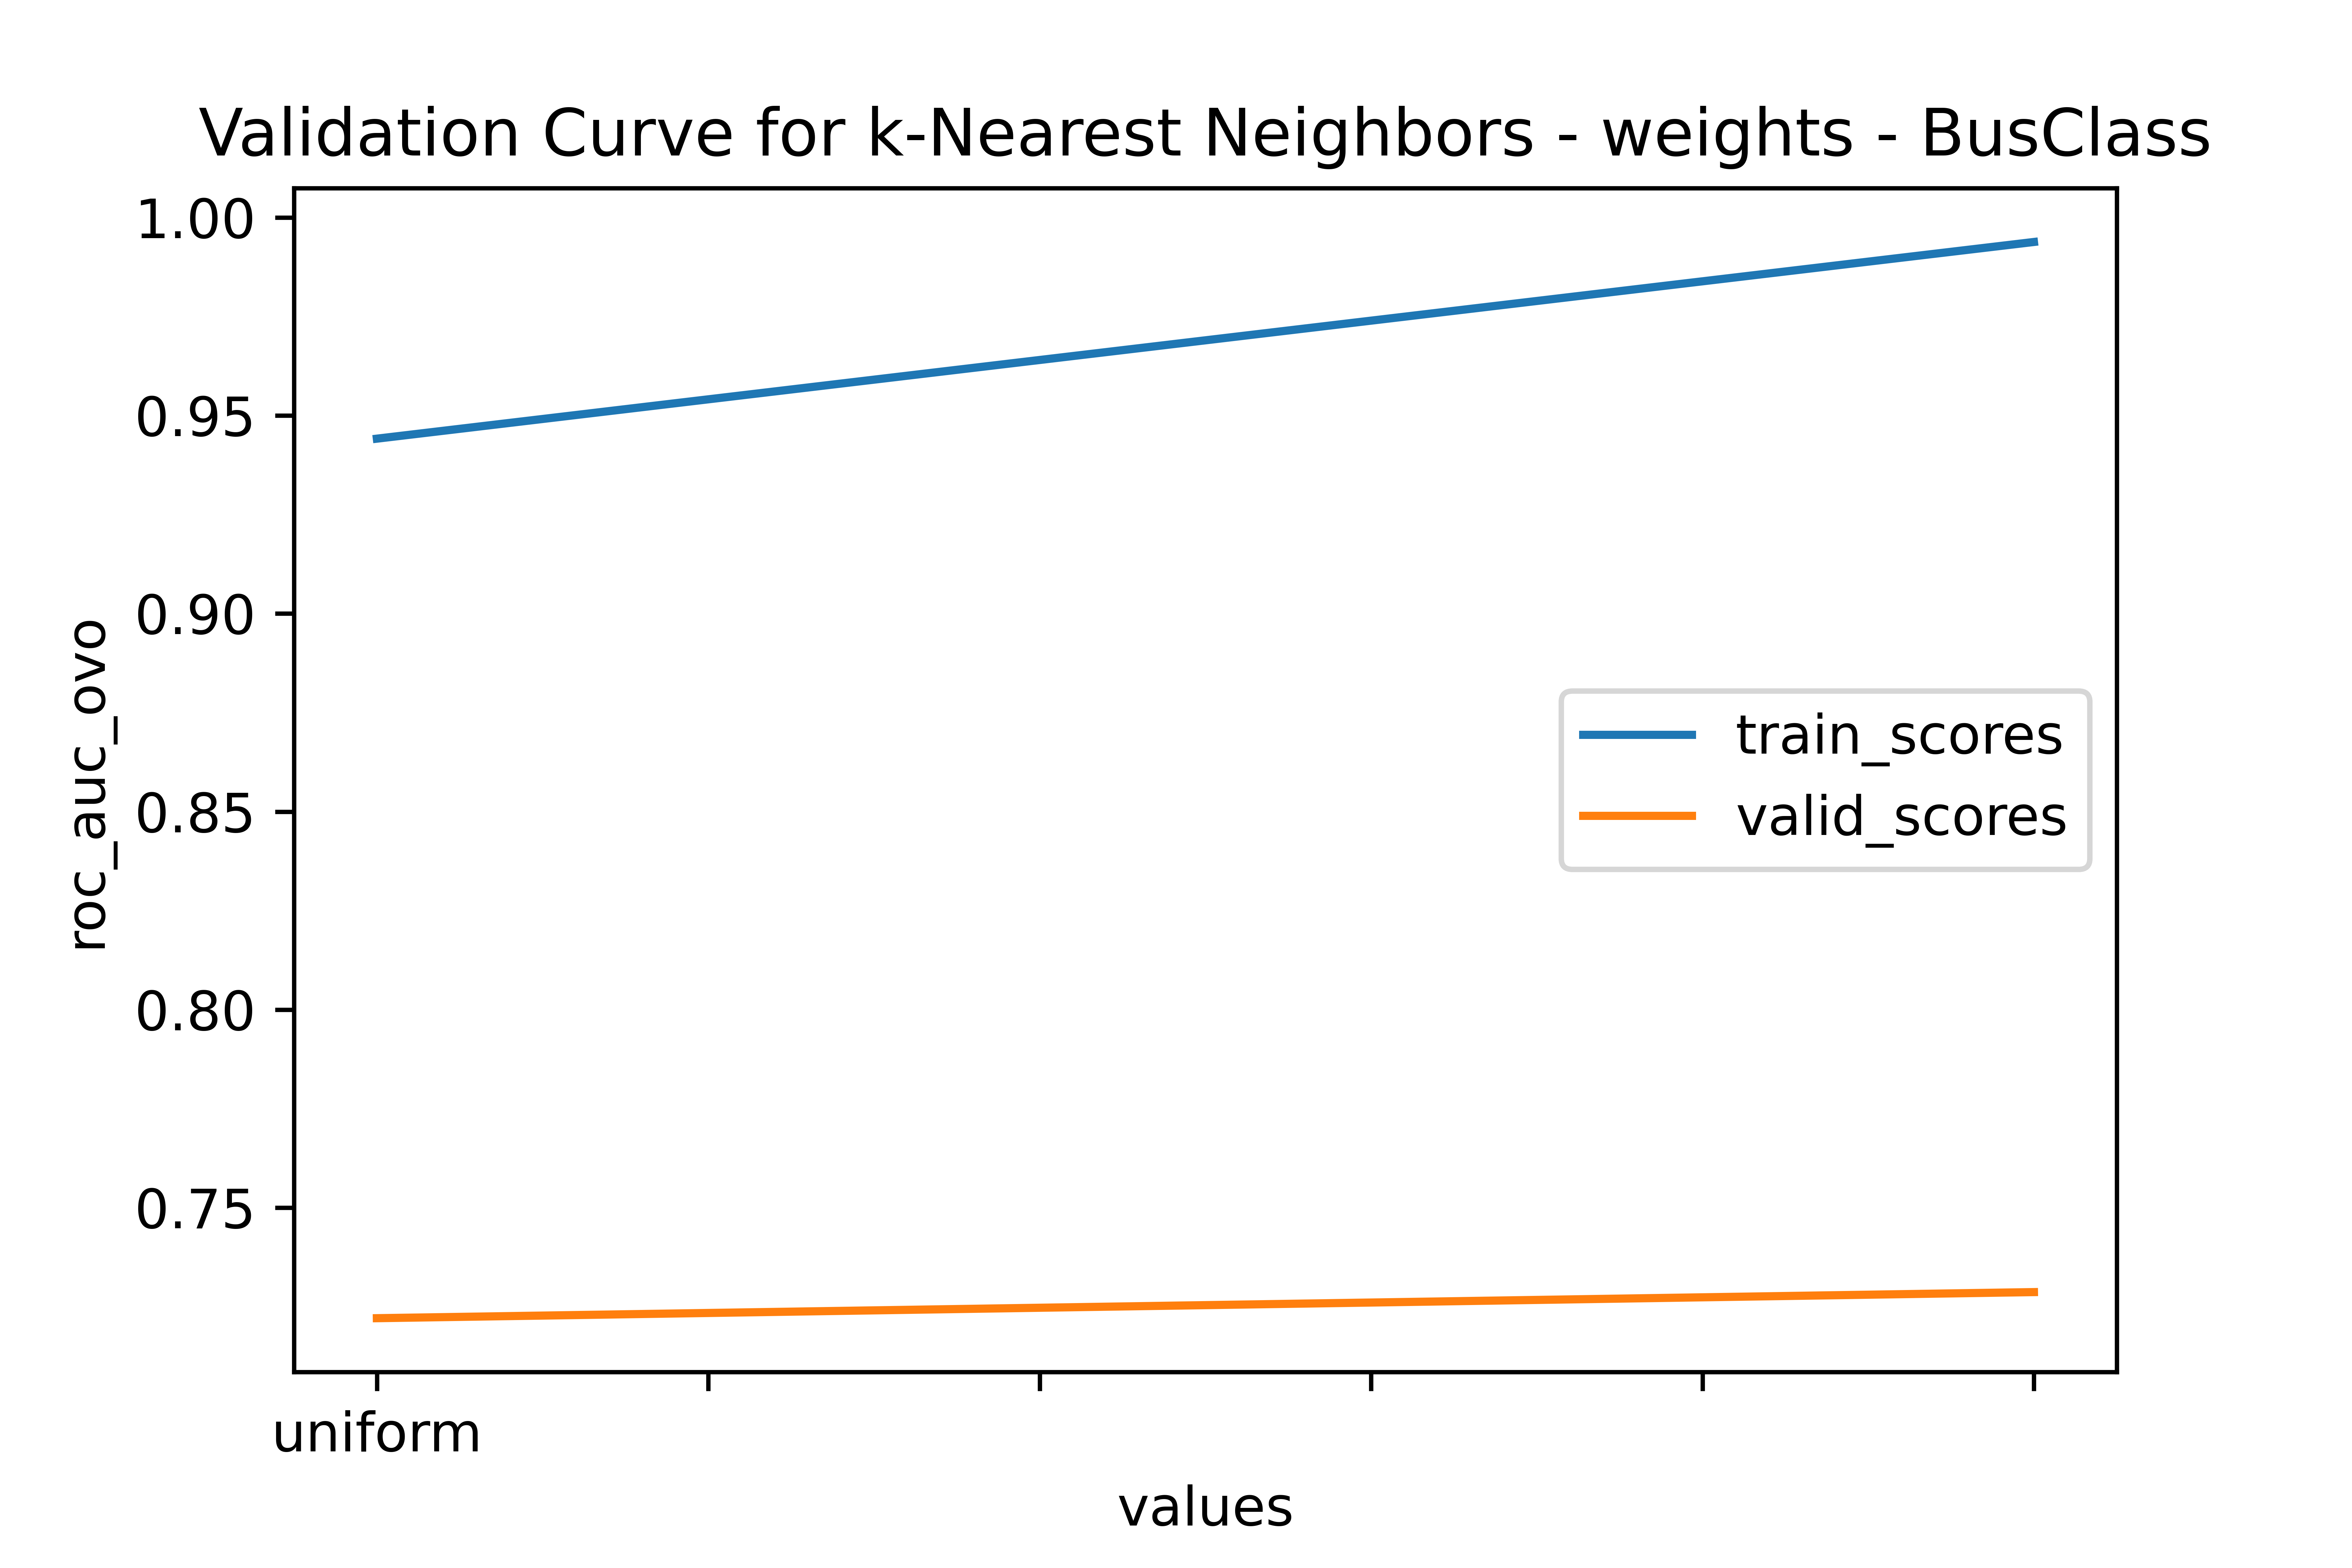
\includegraphics[width=3.4in]{Figures/BusClass-0920/KNN/val_curve_1.png}
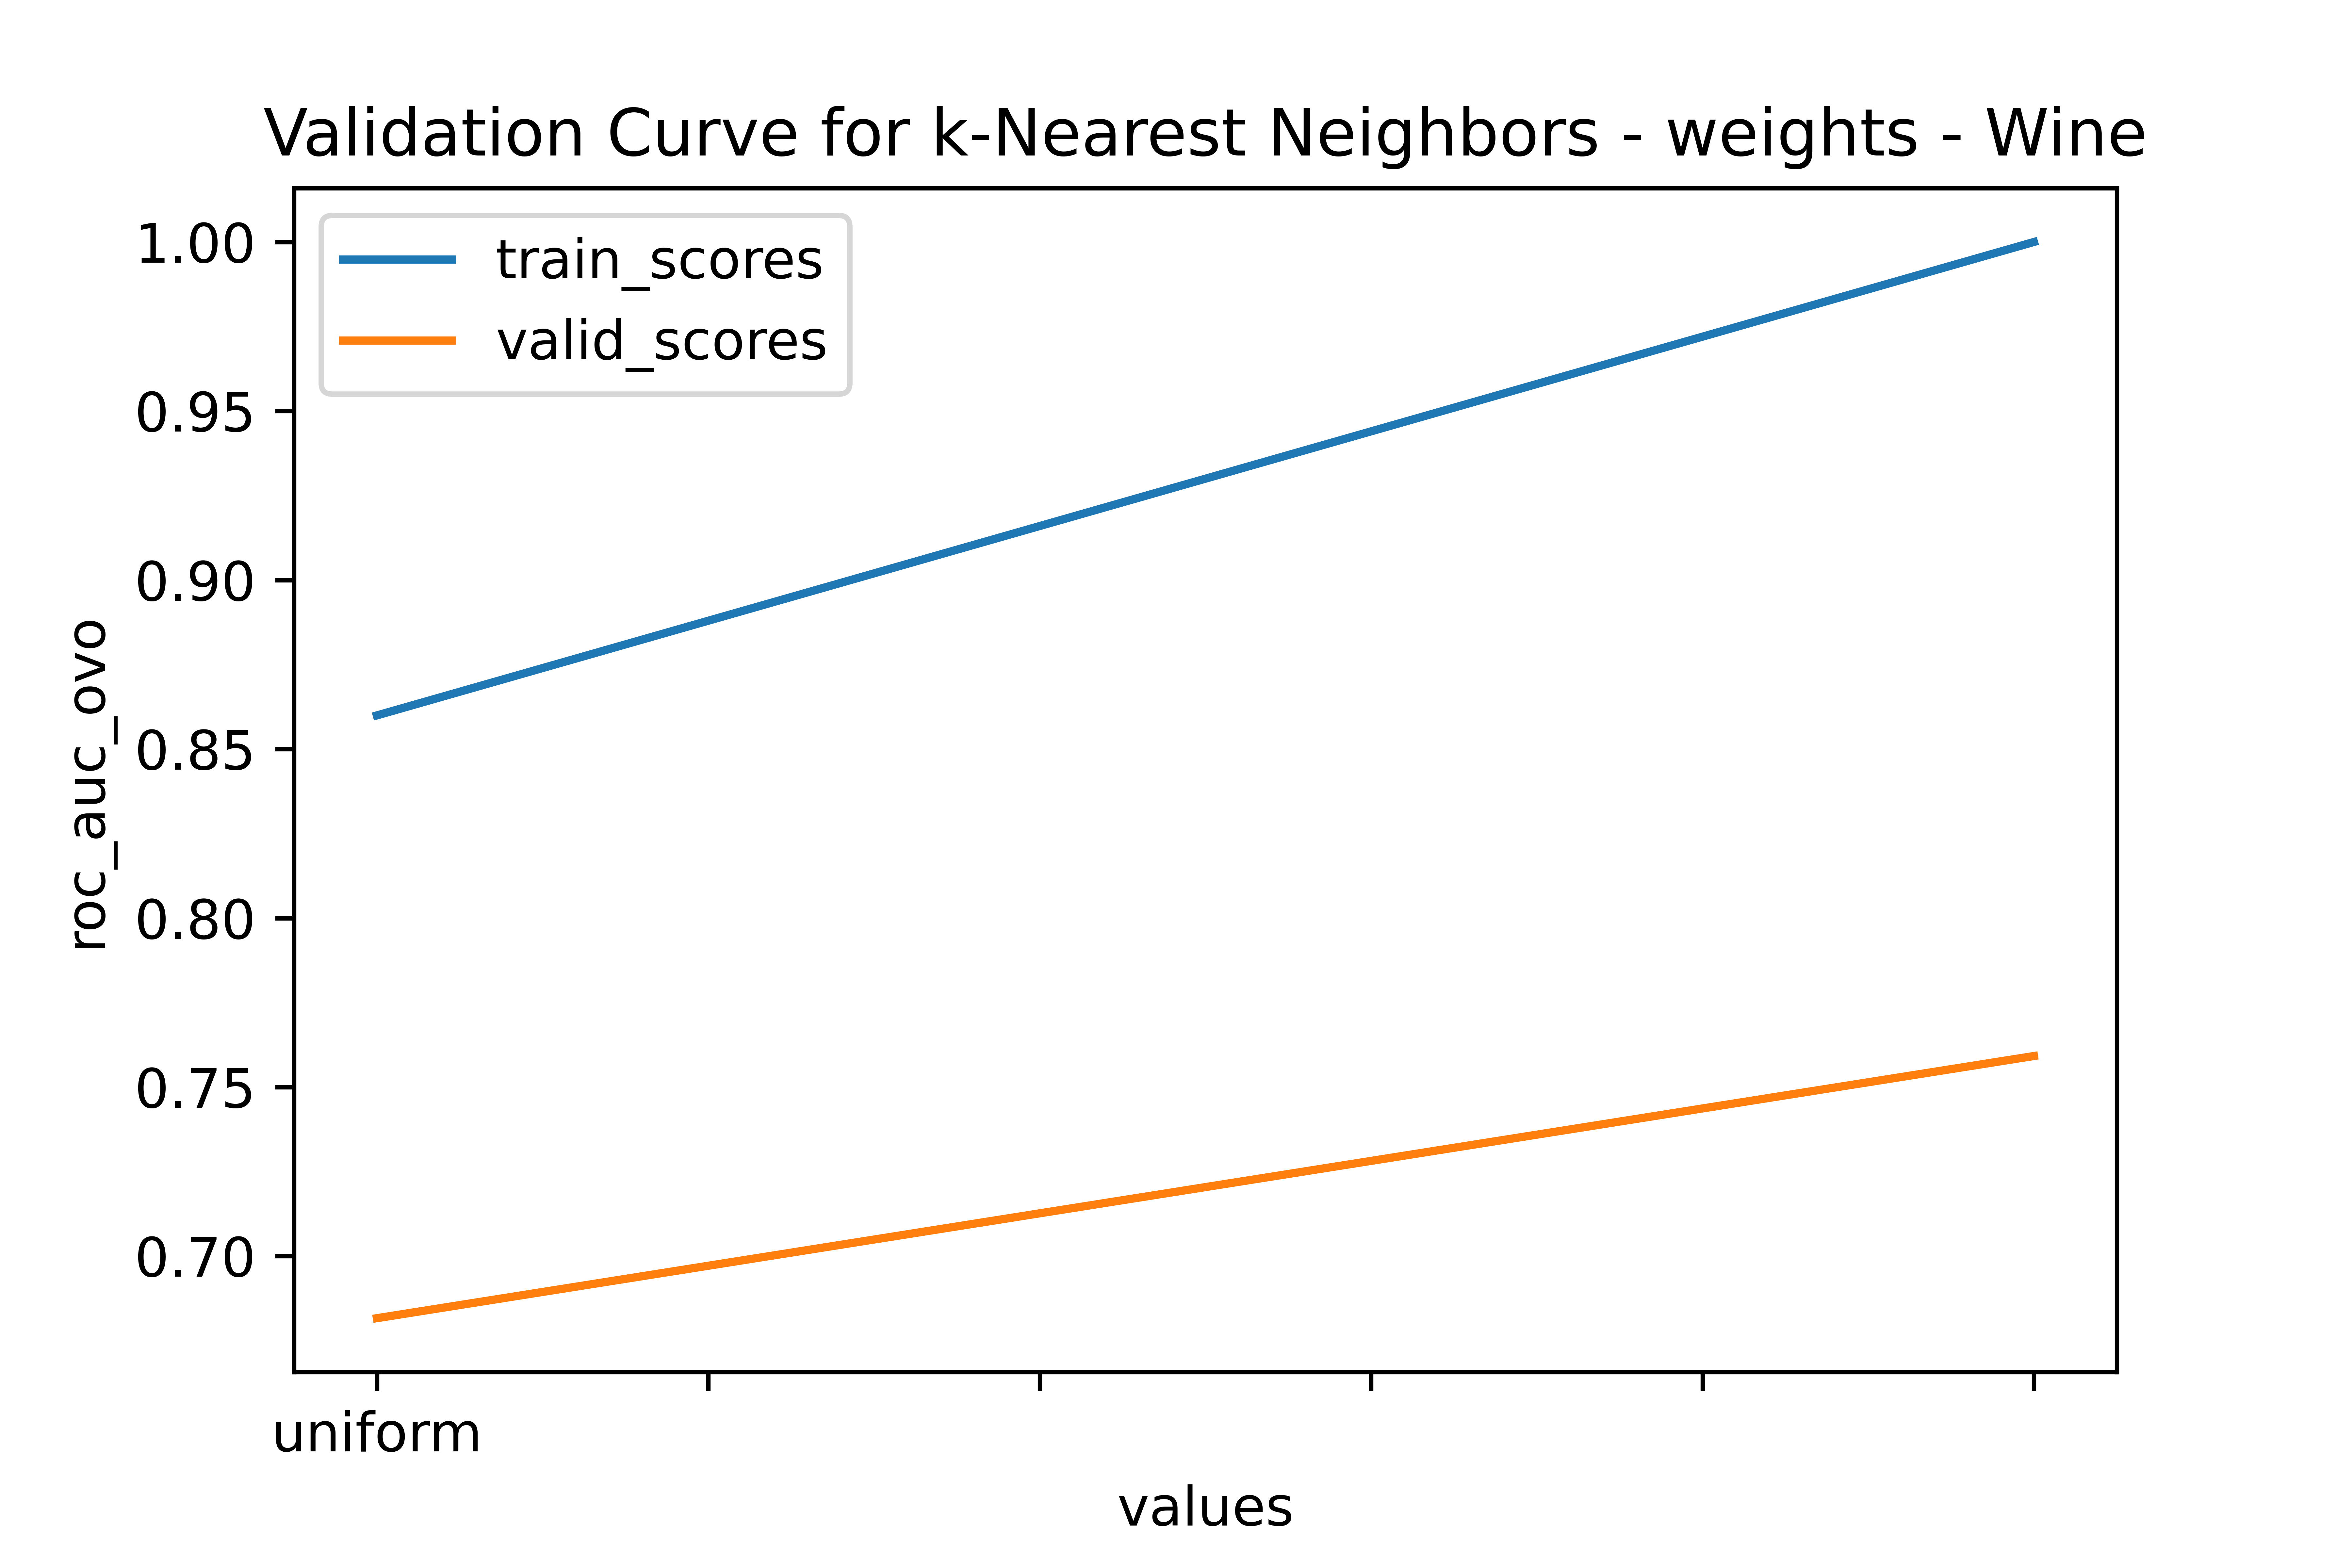
\includegraphics[width=3.4in]{Figures/Wine-0921/KNN/val_curve_1.png}

\subsubsection{Learning Curves}
Both of the learning curves exhibit a remarkably similar shape. It seems that both classifiers could benefit from more data and are, as of yet, still underfit.

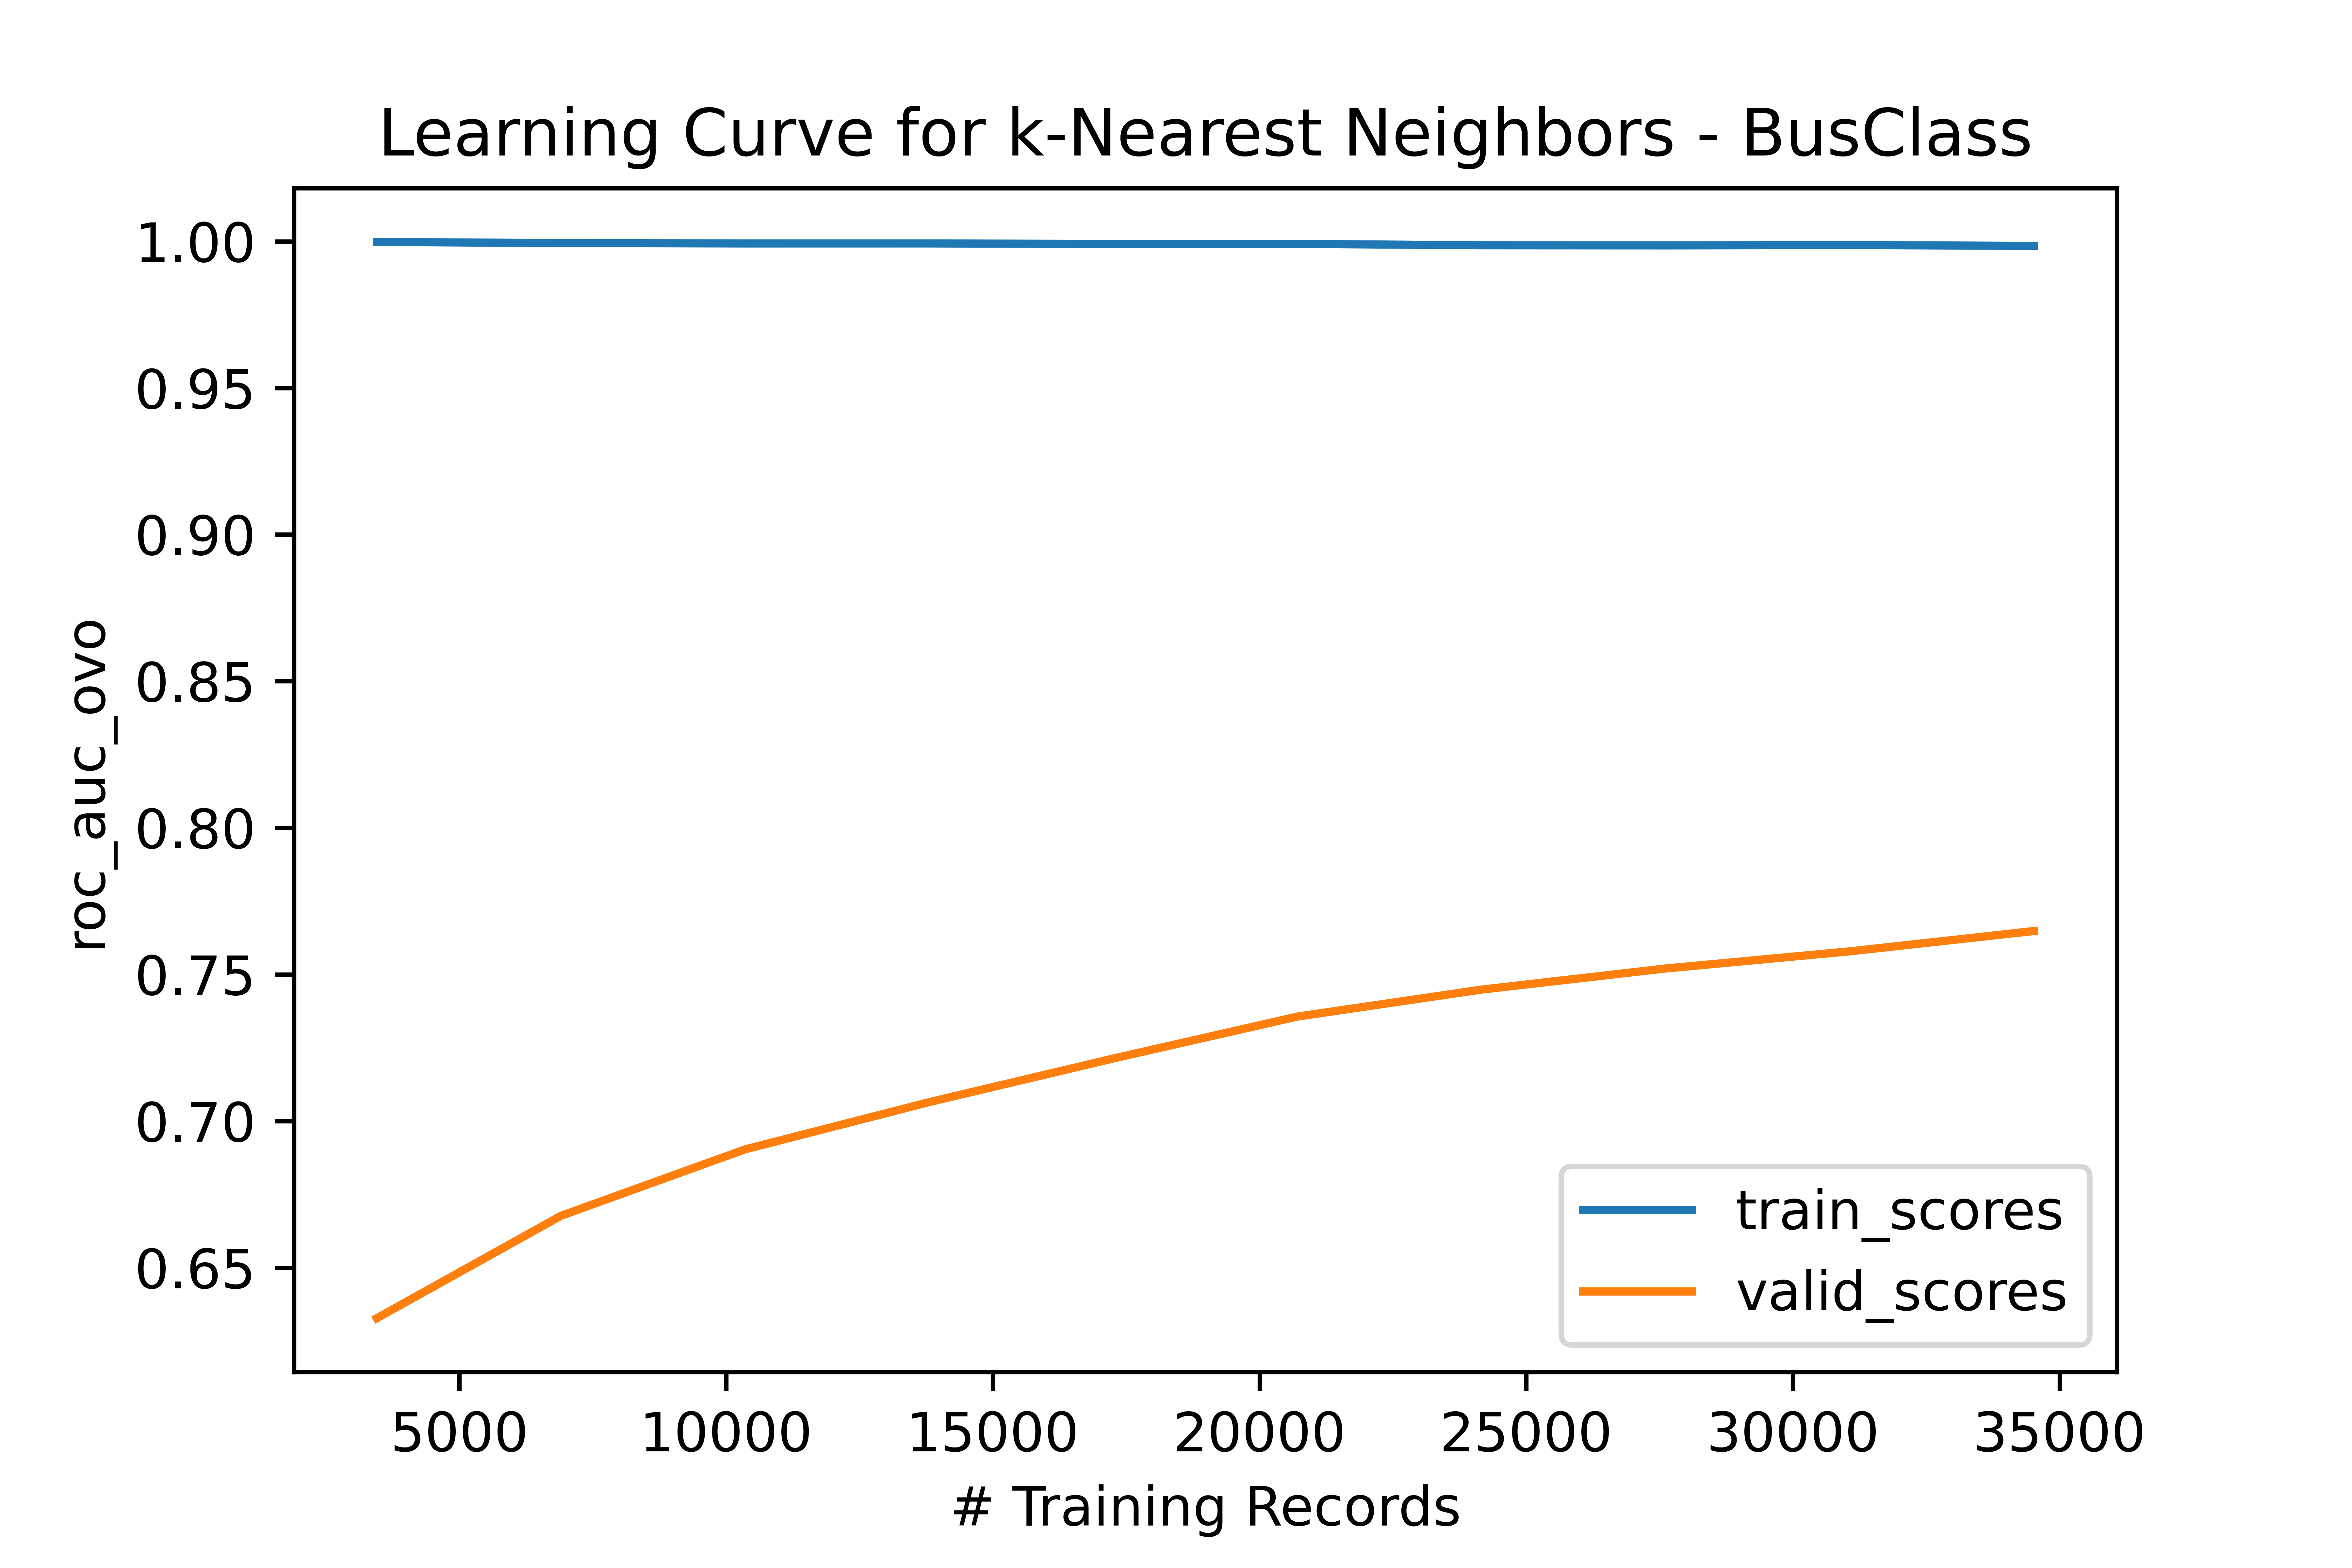
\includegraphics[width=3.4in]{Figures/BusClass-0920/KNN/learn_curve.png}
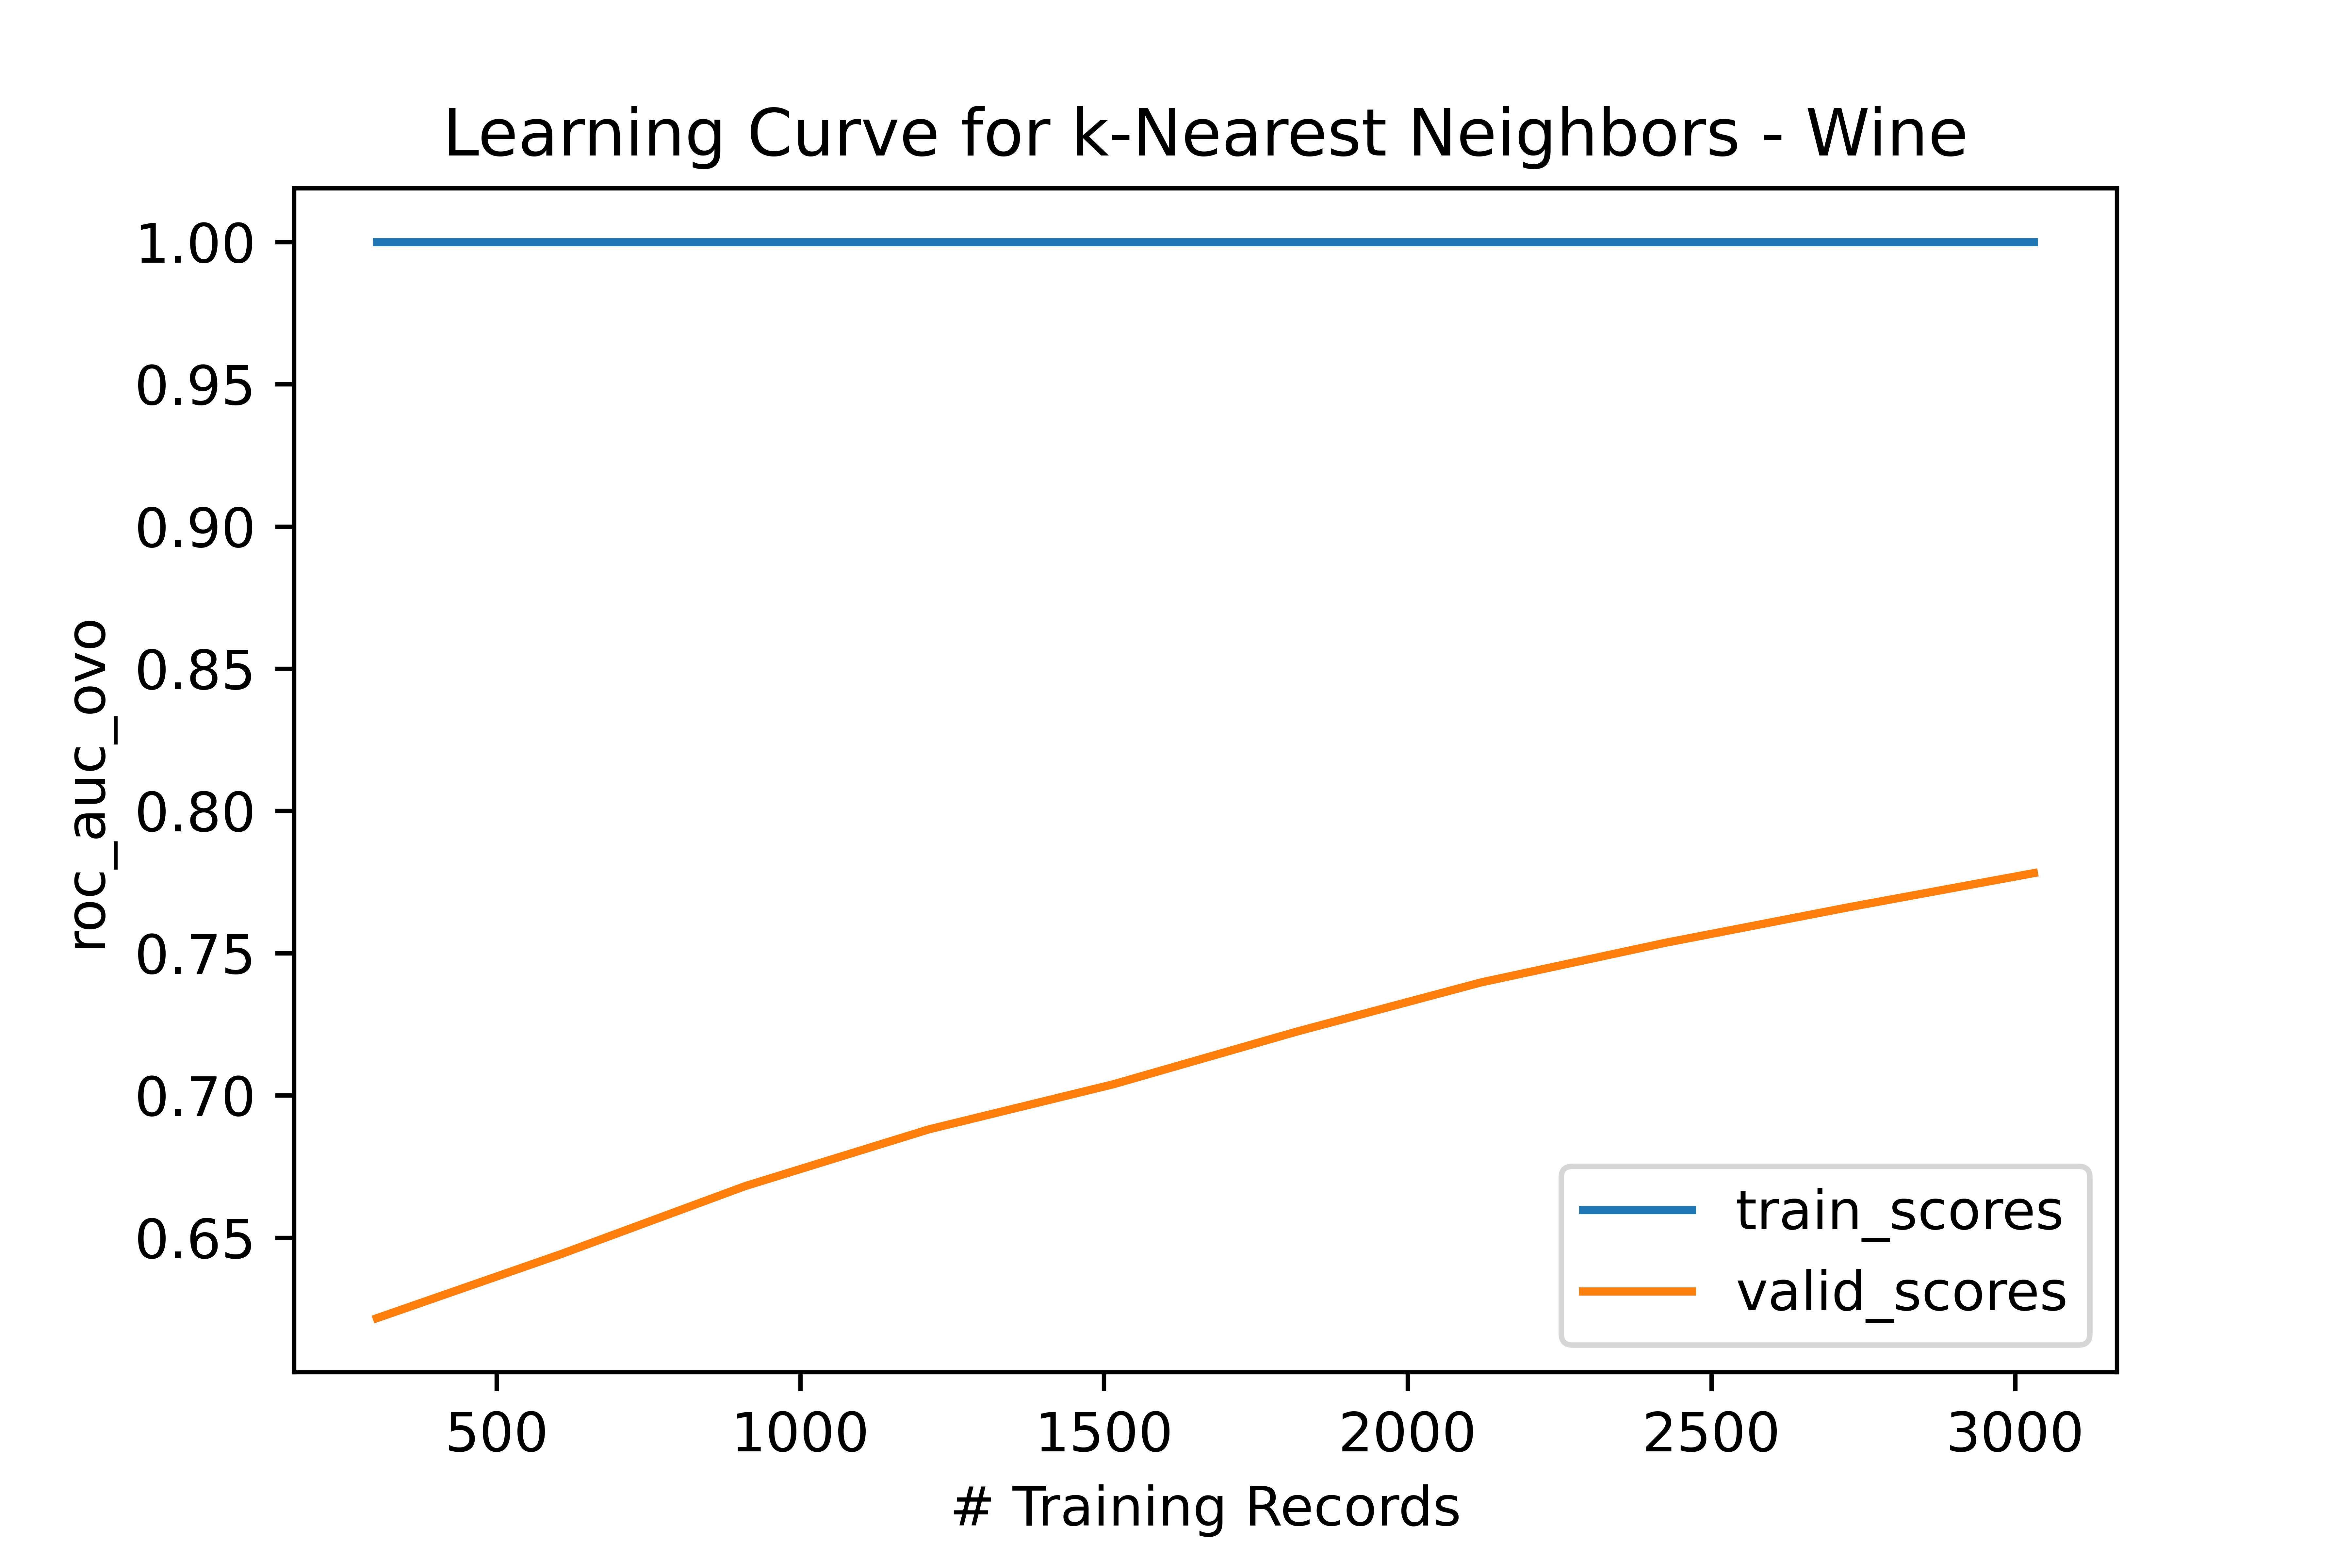
\includegraphics[width=3.4in]{Figures/Wine-0921/KNN/learn_curve.png}

\subsubsection{Wall Clock Time}
Here the timings differ from past algorithms. This makes sense given that there's not much "fitting" go on with the $k$-Nearest Neighbors algorithm. Instead all of the data points are preserved, and the time required to run it involves reviewing all data points and identifying the closest records. This is very costly and scales linearly with training data, at least for the business classification task. The wine dataset is small enough that the score times look constant.

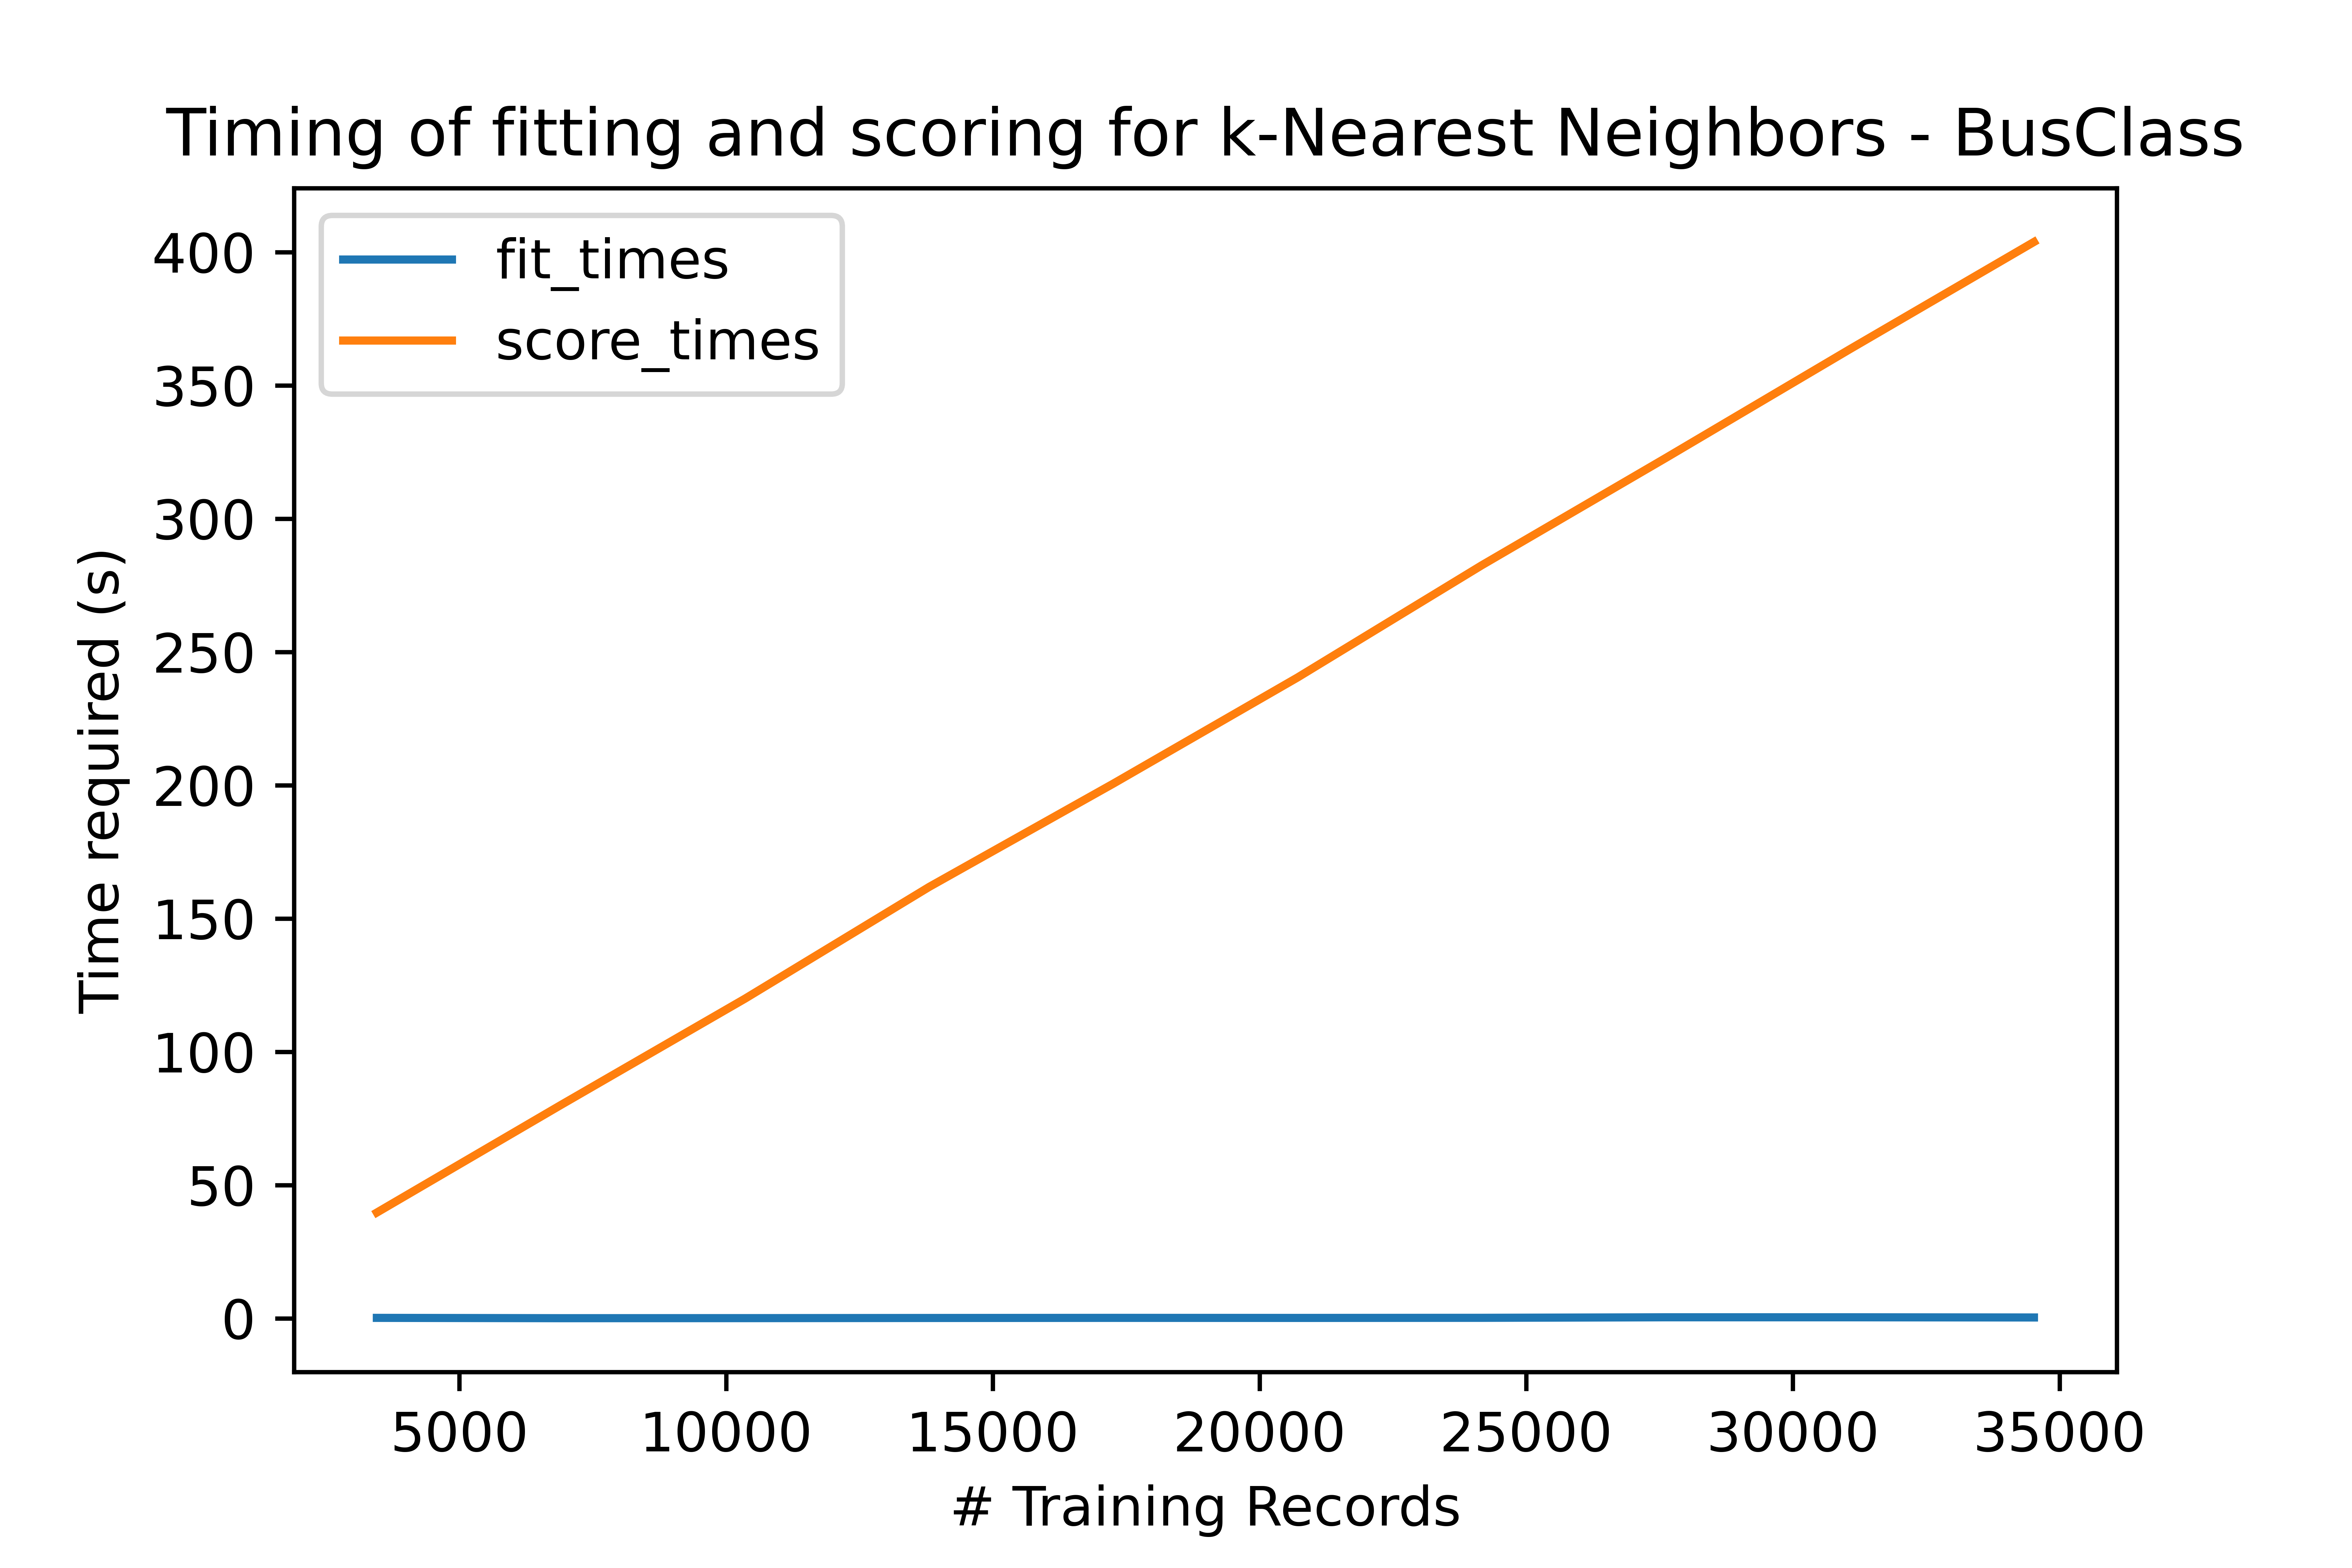
\includegraphics[width=3.4in]{Figures/BusClass-0920/KNN/time_curve.png}
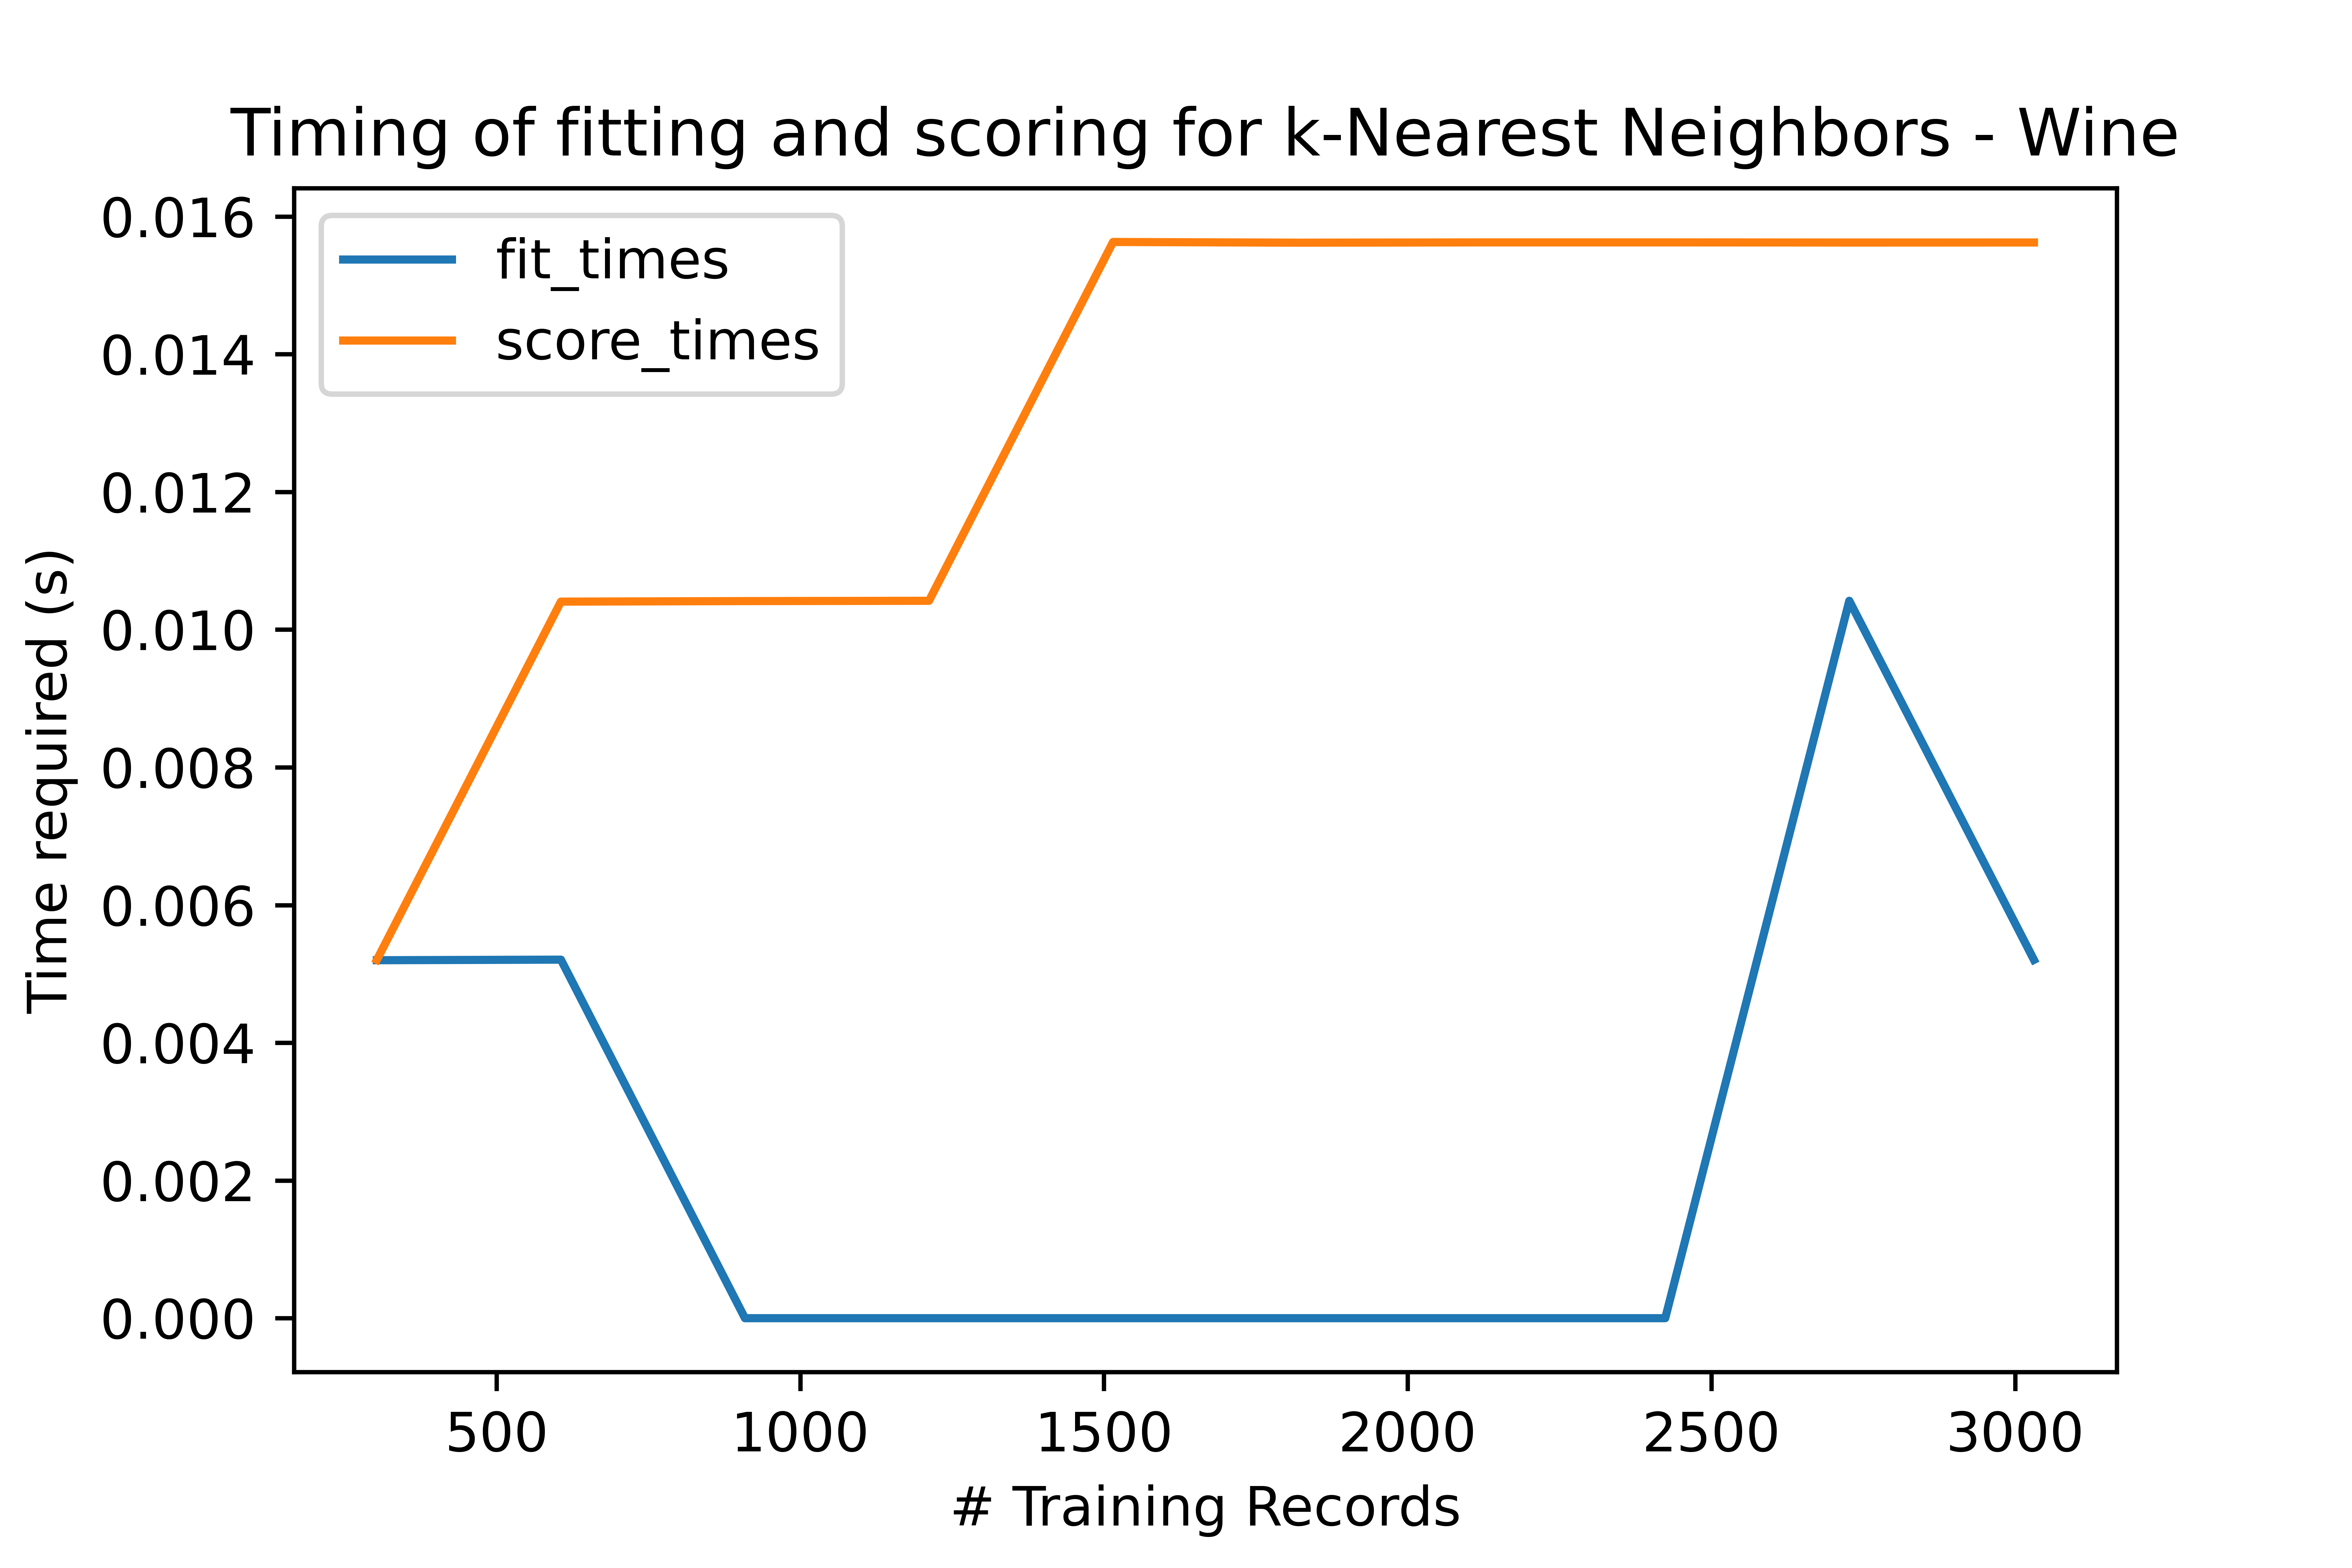
\includegraphics[width=3.4in]{Figures/Wine-0921/KNN/time_curve.png}

\subsection{Performance on Holdout Set}
Let us review what we have learned thus far. Using cross-validation on our training data, we saw that the boosting and neural network algorithms seem to be much stronger on the business classification task. These algorithms were able to achieve a degree of expressiveness that the other ones could not match, which was useful for a design matrix with a thousand columns.

Boosting also came out on top for the wine classification task. In general, I was surprised to see that the wine classifier's performance was not as strong as that of the business classifier. It appeared to be a less complicated dataset with far more meaningful features, though apparently that was not the case.

Using our validation curves, we have learned the optimal model tunings (at least amongst the hyperparameters considered here) and are ready to test the models one last time on our holdout datasets. We first fit on the entire training datasets and then compute the score of the resulting model on our holdout data, where our scoring method is the same as previously. The table below shows the performance metrics on the holdout set.

\begin{table}
\centering
\caption{Holdout OvO AUC Scores}
\begin{tabular}{lrr}
\toprule
{} &  Wine &  BusClass \\
\midrule
\textbf{k-Nearest Neighbors} & 81.6\% &     78.7\% \\
\textbf{Decision Tree      } & 71.8\% &     78.0\% \\
\textbf{Neural Network     } & 75.1\% &     96.9\% \\
\textbf{SVM                } & 54.0\% &     71.3\% \\
\textbf{Boosting           } & 85.5\% &     97.0\% \\
\bottomrule
\end{tabular}
\end{table}

\section{References}
\printbibliography[heading=none]


\end{document}